% Options for packages loaded elsewhere
\PassOptionsToPackage{unicode}{hyperref}
\PassOptionsToPackage{hyphens}{url}
%
\documentclass[
]{book}
\usepackage{amsmath,amssymb}
\usepackage{iftex}
\ifPDFTeX
  \usepackage[T1]{fontenc}
  \usepackage[utf8]{inputenc}
  \usepackage{textcomp} % provide euro and other symbols
\else % if luatex or xetex
  \usepackage{unicode-math} % this also loads fontspec
  \defaultfontfeatures{Scale=MatchLowercase}
  \defaultfontfeatures[\rmfamily]{Ligatures=TeX,Scale=1}
\fi
\usepackage{lmodern}
\ifPDFTeX\else
  % xetex/luatex font selection
\fi
% Use upquote if available, for straight quotes in verbatim environments
\IfFileExists{upquote.sty}{\usepackage{upquote}}{}
\IfFileExists{microtype.sty}{% use microtype if available
  \usepackage[]{microtype}
  \UseMicrotypeSet[protrusion]{basicmath} % disable protrusion for tt fonts
}{}
\makeatletter
\@ifundefined{KOMAClassName}{% if non-KOMA class
  \IfFileExists{parskip.sty}{%
    \usepackage{parskip}
  }{% else
    \setlength{\parindent}{0pt}
    \setlength{\parskip}{6pt plus 2pt minus 1pt}}
}{% if KOMA class
  \KOMAoptions{parskip=half}}
\makeatother
\usepackage{xcolor}
\usepackage{color}
\usepackage{fancyvrb}
\newcommand{\VerbBar}{|}
\newcommand{\VERB}{\Verb[commandchars=\\\{\}]}
\DefineVerbatimEnvironment{Highlighting}{Verbatim}{commandchars=\\\{\}}
% Add ',fontsize=\small' for more characters per line
\usepackage{framed}
\definecolor{shadecolor}{RGB}{248,248,248}
\newenvironment{Shaded}{\begin{snugshade}}{\end{snugshade}}
\newcommand{\AlertTok}[1]{\textcolor[rgb]{0.94,0.16,0.16}{#1}}
\newcommand{\AnnotationTok}[1]{\textcolor[rgb]{0.56,0.35,0.01}{\textbf{\textit{#1}}}}
\newcommand{\AttributeTok}[1]{\textcolor[rgb]{0.13,0.29,0.53}{#1}}
\newcommand{\BaseNTok}[1]{\textcolor[rgb]{0.00,0.00,0.81}{#1}}
\newcommand{\BuiltInTok}[1]{#1}
\newcommand{\CharTok}[1]{\textcolor[rgb]{0.31,0.60,0.02}{#1}}
\newcommand{\CommentTok}[1]{\textcolor[rgb]{0.56,0.35,0.01}{\textit{#1}}}
\newcommand{\CommentVarTok}[1]{\textcolor[rgb]{0.56,0.35,0.01}{\textbf{\textit{#1}}}}
\newcommand{\ConstantTok}[1]{\textcolor[rgb]{0.56,0.35,0.01}{#1}}
\newcommand{\ControlFlowTok}[1]{\textcolor[rgb]{0.13,0.29,0.53}{\textbf{#1}}}
\newcommand{\DataTypeTok}[1]{\textcolor[rgb]{0.13,0.29,0.53}{#1}}
\newcommand{\DecValTok}[1]{\textcolor[rgb]{0.00,0.00,0.81}{#1}}
\newcommand{\DocumentationTok}[1]{\textcolor[rgb]{0.56,0.35,0.01}{\textbf{\textit{#1}}}}
\newcommand{\ErrorTok}[1]{\textcolor[rgb]{0.64,0.00,0.00}{\textbf{#1}}}
\newcommand{\ExtensionTok}[1]{#1}
\newcommand{\FloatTok}[1]{\textcolor[rgb]{0.00,0.00,0.81}{#1}}
\newcommand{\FunctionTok}[1]{\textcolor[rgb]{0.13,0.29,0.53}{\textbf{#1}}}
\newcommand{\ImportTok}[1]{#1}
\newcommand{\InformationTok}[1]{\textcolor[rgb]{0.56,0.35,0.01}{\textbf{\textit{#1}}}}
\newcommand{\KeywordTok}[1]{\textcolor[rgb]{0.13,0.29,0.53}{\textbf{#1}}}
\newcommand{\NormalTok}[1]{#1}
\newcommand{\OperatorTok}[1]{\textcolor[rgb]{0.81,0.36,0.00}{\textbf{#1}}}
\newcommand{\OtherTok}[1]{\textcolor[rgb]{0.56,0.35,0.01}{#1}}
\newcommand{\PreprocessorTok}[1]{\textcolor[rgb]{0.56,0.35,0.01}{\textit{#1}}}
\newcommand{\RegionMarkerTok}[1]{#1}
\newcommand{\SpecialCharTok}[1]{\textcolor[rgb]{0.81,0.36,0.00}{\textbf{#1}}}
\newcommand{\SpecialStringTok}[1]{\textcolor[rgb]{0.31,0.60,0.02}{#1}}
\newcommand{\StringTok}[1]{\textcolor[rgb]{0.31,0.60,0.02}{#1}}
\newcommand{\VariableTok}[1]{\textcolor[rgb]{0.00,0.00,0.00}{#1}}
\newcommand{\VerbatimStringTok}[1]{\textcolor[rgb]{0.31,0.60,0.02}{#1}}
\newcommand{\WarningTok}[1]{\textcolor[rgb]{0.56,0.35,0.01}{\textbf{\textit{#1}}}}
\usepackage{longtable,booktabs,array}
\usepackage{calc} % for calculating minipage widths
% Correct order of tables after \paragraph or \subparagraph
\usepackage{etoolbox}
\makeatletter
\patchcmd\longtable{\par}{\if@noskipsec\mbox{}\fi\par}{}{}
\makeatother
% Allow footnotes in longtable head/foot
\IfFileExists{footnotehyper.sty}{\usepackage{footnotehyper}}{\usepackage{footnote}}
\makesavenoteenv{longtable}
\usepackage{graphicx}
\makeatletter
\def\maxwidth{\ifdim\Gin@nat@width>\linewidth\linewidth\else\Gin@nat@width\fi}
\def\maxheight{\ifdim\Gin@nat@height>\textheight\textheight\else\Gin@nat@height\fi}
\makeatother
% Scale images if necessary, so that they will not overflow the page
% margins by default, and it is still possible to overwrite the defaults
% using explicit options in \includegraphics[width, height, ...]{}
\setkeys{Gin}{width=\maxwidth,height=\maxheight,keepaspectratio}
% Set default figure placement to htbp
\makeatletter
\def\fps@figure{htbp}
\makeatother
\setlength{\emergencystretch}{3em} % prevent overfull lines
\providecommand{\tightlist}{%
  \setlength{\itemsep}{0pt}\setlength{\parskip}{0pt}}
\setcounter{secnumdepth}{5}
\usepackage{booktabs}
\ifLuaTeX
  \usepackage{selnolig}  % disable illegal ligatures
\fi
\usepackage[]{natbib}
\bibliographystyle{apalike}
\IfFileExists{bookmark.sty}{\usepackage{bookmark}}{\usepackage{hyperref}}
\IfFileExists{xurl.sty}{\usepackage{xurl}}{} % add URL line breaks if available
\urlstyle{same}
\hypersetup{
  pdftitle={Social Media Analytics},
  pdfauthor={AP Leith},
  hidelinks,
  pdfcreator={LaTeX via pandoc}}

\title{Social Media Analytics}
\usepackage{etoolbox}
\makeatletter
\providecommand{\subtitle}[1]{% add subtitle to \maketitle
  \apptocmd{\@title}{\par {\large #1 \par}}{}{}
}
\makeatother
\subtitle{An R Guide for Media Researchers}
\author{AP Leith\footnote{Southern Illinois University Edwardsville, \href{mailto:aleith@siue.edu}{\nolinkurl{aleith@siue.edu}}}}
\date{2024-04-16}

\begin{document}
\maketitle

{
\setcounter{tocdepth}{1}
\tableofcontents
}
\hypertarget{preface}{%
\chapter*{Preface}\label{preface}}
\addcontentsline{toc}{chapter}{Preface}

Welcome to ``Social Media Analytics: An R Guide for Media Researchers,'' a comprehensive guide designed to navigate the intricate pathways of social media analytics in the ever-evolving field of mass communications. This textbook is a culmination of my journey in academia and a reflection of my commitment to advancing the understanding of social media analytics, particularly through the lens of quantitative analysis using R and RStudio.

This book heavily leans on American-dominant social network sites in its discussions on social media. This will not be permanent as future iterations of this text will expand to include more global examples tha include social media beyond social networking sites.

I am Dr.~Alex P. Leith, currently serving as an Assistant Professor in the Department of Mass Communications at Southern Illinois University Edwardsville. My academic journey, which began with a Ph.D.~in Information and Media from Michigan State University, has been a blend of rigorous research and practical application in the fields of digital media, virtual reality, and the social dimensions of digital media. My dissertation, ``Gameplay Livestreaming: Agents of Gamespace,'' set the stage for my ongoing exploration of contemporary digital media trends.

My professional trajectory has been diverse, encompassing roles as a Graduate Assistant at Michigan State University, an Adjunct Instructor at McKendree University and St.~Louis College of Pharmacy, and a Marketing Manager at Brigham Young University -- Idaho. These experiences have enriched my understanding of the multifaceted nature of mass communications, both in academic and practical contexts.

This textbook is a unique endeavor, coalesced with the assistance of ChatGPT 4, a state-of-the-art language model developed by OpenAI. The collaboration with ChatGPT 4 has enabled the integration of advanced AI insights into the book's development, ensuring a blend of human expertise and technological innovation.

``Quantitative Research in Mass Communications'' is structured to guide readers from the foundational aspects of mass communication research and ethics, through the complexities of IRB certification, to the development of research interests and the intricacies of conducting literature reviews. It further delves into the practicalities of formulating research questions, designing quantitative studies, and harnessing the power of R and RStudio for data management, analysis, and visualization. The book culminates with insights into engaging public audiences, writing for them, and presenting research findings effectively.

My research, reflected in publications like ``Psychology of Popular Media'' and ``IEEE Transactions on Games,'' and my success in securing funding for research projects have significantly influenced the content of this textbook. The book aims not only to impart knowledge but also to inspire innovation and critical thinking in the field of mass communications.

As readers embark on this journey through ``Quantitative Research in Mass Communications,'' my hope is that this textbook serves as a valuable resource, aiding in the development of skilled, insightful, and ethically grounded researchers in the dynamic realm of mass communications.

Dr.~Alex P. Leith
Assistant Professor
Department of Mass Communications
Southern Illinois University Edwardsville

\hypertarget{introduction-to-social-media-types}{%
\chapter{Introduction to Social Media Types}\label{introduction-to-social-media-types}}

\hypertarget{overview-of-different-social-media-platforms}{%
\section*{Overview of Different Social Media Platforms}\label{overview-of-different-social-media-platforms}}
\addcontentsline{toc}{section}{Overview of Different Social Media Platforms}

Social media has evolved into a complex ecosystem, each platform with its unique culture, demographic, and influence. Understanding these platforms' characteristics is crucial for navigating the social media landscape effectively, whether for personal use, marketing, or research. This section provides an overview of various social media platforms, their comparative features, historical evolution, cultural nuances, and their broader impact on media and communication.

\hypertarget{introduction}{%
\subsection*{Introduction}\label{introduction}}
\addcontentsline{toc}{subsection}{Introduction}

\begin{itemize}
\tightlist
\item
  \textbf{Defining Social Media}: The section begins by defining social media as digital platforms that facilitate the creation, sharing, and exchange of content, ideas, career interests, and other forms of expression via virtual communities and networks.
\item
  \textbf{Role in Contemporary Society}: It would highlight social media's role in today's society, touching upon its impact on communication, information dissemination, networking, and entertainment.
\end{itemize}

\hypertarget{comparative-analysis-of-platforms}{%
\subsection*{Comparative Analysis of Platforms}\label{comparative-analysis-of-platforms}}
\addcontentsline{toc}{subsection}{Comparative Analysis of Platforms}

\begin{itemize}
\tightlist
\item
  \textbf{Facebook}: As one of the oldest and most diverse platforms, Facebook is characterized by its broad user base and features that cater to personal networking, business promotion, entertainment, and news dissemination.
\item
  \textbf{Twitter}: Known for its brevity and immediacy, Twitter serves as a platform for real-time updates, public discourse, and a significant channel for news and political commentary.
\item
  \textbf{Instagram}: Focused on visual content, Instagram is popular for its photo and video sharing capabilities, appealing largely to a younger demographic seeking creative expression and lifestyle inspiration.
\item
  \textbf{LinkedIn}: This platform stands out for its professional networking focus, connecting individuals and organizations for career-related purposes, industry discussions, and corporate branding.
\item
  \textbf{TikTok}: A newer entrant, TikTok has rapidly gained popularity for its short-form video content, appealing particularly to Gen Z users with its entertainment-focused and interactive content.
\end{itemize}

\hypertarget{historical-context}{%
\subsection*{Historical Context}\label{historical-context}}
\addcontentsline{toc}{subsection}{Historical Context}

\begin{itemize}
\tightlist
\item
  \textbf{Evolution of Platforms}: The section would trace the evolution of these platforms, noting key developmental milestones such as Facebook's expansion from a college network to a global platform, Twitter's role in social movements, and LinkedIn's progression in professional networking.
\item
  \textbf{Technological Advancements}: The role of technological advancements in shaping these platforms, such as the integration of AI in content curation and the rise of mobile computing influencing platform accessibility and user experience.
\end{itemize}

\hypertarget{platform-specific-culture-and-etiquette}{%
\subsection*{Platform-Specific Culture and Etiquette}\label{platform-specific-culture-and-etiquette}}
\addcontentsline{toc}{subsection}{Platform-Specific Culture and Etiquette}

\begin{itemize}
\tightlist
\item
  \textbf{Cultural Nuances}: Each platform's unique cultural nuances, like Twitter's hashtag culture facilitating global conversations, Instagram's emphasis on aesthetics, and LinkedIn's formal and professional tone.
\item
  \textbf{Etiquette and Best Practices}: Discussing the unwritten rules and etiquette specific to each platform, such as the appropriate use of emojis on Instagram, the tone of conversations on LinkedIn, and the character limit discipline on Twitter.
\end{itemize}

\hypertarget{impact-on-media-and-communication}{%
\subsection*{Impact on Media and Communication}\label{impact-on-media-and-communication}}
\addcontentsline{toc}{subsection}{Impact on Media and Communication}

\begin{itemize}
\tightlist
\item
  \textbf{Influencing Journalism and News}: Analyzing how platforms like Twitter and Facebook have become significant sources of news, influencing journalism practices and the spread of information.
\item
  \textbf{Changing Personal Communication}: Discussing the shift in personal communication dynamics, particularly highlighting platforms like Instagram and Snapchat that emphasize visual communication.
\item
  \textbf{Marketing and Branding}: The role of these platforms in transforming marketing strategies, with a focus on targeted advertising, influencer marketing, and brand engagement.
\item
  \textbf{Political Discourse and Movements}: Addressing the influence of social media in political discourse, activism, and social movements, noting the role of platforms in mobilizing public opinion and activism.
\end{itemize}

\hypertarget{types-of-data-generated-by-each-platform}{%
\section*{Types of Data Generated by Each Platform}\label{types-of-data-generated-by-each-platform}}
\addcontentsline{toc}{section}{Types of Data Generated by Each Platform}

In the realm of social media, various types of data are generated daily, each offering unique insights into user behaviors, preferences, and interactions. Understanding the nature of this data and how it is generated across different platforms is crucial for effective analysis and strategy development in social media analytics. This section provides a comprehensive overview of the types of data generated by each platform, their characteristics, the interplay between data generation and user behavior, and the analytical approaches suited to different data types.

\hypertarget{overview-of-social-media-data}{%
\subsection*{Overview of Social Media Data}\label{overview-of-social-media-data}}
\addcontentsline{toc}{subsection}{Overview of Social Media Data}

\begin{itemize}
\tightlist
\item
  \textbf{Categorization of Data}: Introducing the broad categories of data typically found on social media platforms. This includes textual content (posts, tweets, comments), visual content (images, videos), user interactions (likes, shares, comments, views), and metadata (timestamps, geolocation, user demographics).
\item
  \textbf{Significance of Different Data Types}: Highlighting the significance of each data type in understanding user engagement, content popularity, and overall platform dynamics.
\end{itemize}

\hypertarget{data-characteristics-per-platform}{%
\subsection*{Data Characteristics per Platform}\label{data-characteristics-per-platform}}
\addcontentsline{toc}{subsection}{Data Characteristics per Platform}

\begin{itemize}
\tightlist
\item
  \textbf{Instagram and Pinterest}: Focused on visual content, these platforms predominantly generate image and video data. This includes user-posted photos and videos, with accompanying textual descriptions and user engagement metrics like likes, comments, and shares.
\item
  \textbf{Twitter}: Characterized by its textual data, Twitter generates short-form text posts (tweets), including hashtags, mentions, and URLs. Metadata such as retweets and likes are crucial for understanding content reach and impact.
\item
  \textbf{YouTube}: Primarily a platform for video content, YouTube generates data that includes video files, view counts, likes/dislikes, comments, and detailed viewer engagement metrics like watch time and drop-off rates.
\item
  \textbf{Facebook}: A mix of text, images, and videos, Facebook's data complexity includes user posts, reactions (likes, loves, etc.), comments, and shares. Metadata here also encompasses user demographic information and interaction timestamps.
\end{itemize}

\hypertarget{data-generation-and-user-behavior}{%
\subsection*{Data Generation and User Behavior}\label{data-generation-and-user-behavior}}
\addcontentsline{toc}{subsection}{Data Generation and User Behavior}

\begin{itemize}
\tightlist
\item
  \textbf{User Interactions and Content Creation}: Analyzing how user behaviors contribute to data generation. This includes patterns in content creation, sharing behaviors, and engagement trends across different platforms.
\item
  \textbf{Dynamics of Engagement}: Discussing the dynamics behind likes, shares, comments, and views, and how these actions contribute to the broader social media ecosystem.
\item
  \textbf{Trends Influencing Data Generation}: Examining current trends in content creation and sharing, such as the rise of short-form videos on TikTok or the use of stories on Instagram and Facebook.
\end{itemize}

\hypertarget{analytical-approaches-for-different-data-types}{%
\subsection*{Analytical Approaches for Different Data Types}\label{analytical-approaches-for-different-data-types}}
\addcontentsline{toc}{subsection}{Analytical Approaches for Different Data Types}

\begin{itemize}
\tightlist
\item
  \textbf{Textual Analysis}: Approaches like sentiment analysis, content categorization, and trend analysis for textual data, primarily for platforms like Twitter and Facebook.
\item
  \textbf{Image and Video Analysis}: Discussing the techniques for analyzing visual content, including image recognition, video analysis, and engagement patterns, particularly relevant for Instagram, Pinterest, and YouTube.
\item
  \textbf{Engagement and Metadata Analysis}: Techniques for analyzing user interactions and metadata, such as engagement rate calculations, trend analyses based on likes/shares, and user demographic analysis.
\item
  \textbf{Cross-Platform Analysis}: Exploring methods for integrating and analyzing data across different platforms to gain a comprehensive understanding of user behavior and content performance.
\end{itemize}

\hypertarget{the-evolution-of-social-media}{%
\section*{The Evolution of Social Media}\label{the-evolution-of-social-media}}
\addcontentsline{toc}{section}{The Evolution of Social Media}

The landscape of social media has undergone significant transformations since its inception. This evolution is not just a testament to technological advancements but also reflects the changing dynamics of culture, society, and communication. Understanding this evolution is crucial for comprehending the current state and future direction of social media. This section explores the journey from the early beginnings of social media to its current form, the technological advancements that have shaped it, its impact on society and culture, and potential future developments.

\hypertarget{early-beginnings-to-current-state}{%
\subsection*{Early Beginnings to Current State}\label{early-beginnings-to-current-state}}
\addcontentsline{toc}{subsection}{Early Beginnings to Current State}

\begin{itemize}
\tightlist
\item
  \textbf{Origins in Online Forums and Bulletin Boards}: Tracing the roots of social media back to the 1980s and 1990s with the advent of online forums and bulletin board systems (BBS) which allowed users to communicate and share information.
\item
  \textbf{Rise of Early Social Media Platforms}: Discussing the emergence of early social networking sites like Friendster and MySpace in the early 2000s, which introduced the concept of personal profiles and network building.
\item
  \textbf{Dominance of Facebook and Twitter}: Analyzing the rise of Facebook and Twitter, which revolutionized social media by fostering broader connectivity and real-time communication, setting new standards for user engagement and content sharing.
\item
  \textbf{Advent of Mobile-Centric Platforms}: Exploring the emergence of mobile-centric platforms like Snapchat and Instagram, highlighting how the rise of smartphones transformed user interaction and content consumption.
\item
  \textbf{Proliferation of Video Content}: Discussing the increasing dominance of video content with platforms like YouTube, TikTok, and Instagram Reels, which have become central to the contemporary social media experience.
\end{itemize}

\hypertarget{technological-advancements}{%
\subsection*{Technological Advancements}\label{technological-advancements}}
\addcontentsline{toc}{subsection}{Technological Advancements}

\begin{itemize}
\tightlist
\item
  \textbf{Role of Mobile Computing}: Examining how the proliferation of smartphones and mobile applications has significantly impacted social media usage, making it a ubiquitous and integral part of daily life.
\item
  \textbf{Integration of AI and Algorithms}: Discussing the integration of artificial intelligence and sophisticated algorithms for content recommendation, personalized feeds, and targeted advertising, dramatically altering user experience and engagement.
\item
  \textbf{Emergence of AR/VR}: Analyzing the incorporation of augmented reality (AR) and virtual reality (VR) in platforms like Instagram and Snapchat, which has introduced new forms of interactive and immersive content.
\end{itemize}

\hypertarget{cultural-and-societal-impact}{%
\subsection*{Cultural and Societal Impact}\label{cultural-and-societal-impact}}
\addcontentsline{toc}{subsection}{Cultural and Societal Impact}

\begin{itemize}
\tightlist
\item
  \textbf{Social Media in Political Movements}: Assessing the role of social media in facilitating political movements and activism, exemplified by events like the Arab Spring and the Black Lives Matter movement.
\item
  \textbf{Influence on Public Opinion}: Discussing how social media has become a powerful tool in shaping public opinion, with the ability to rapidly disseminate information and mobilize public sentiment.
\item
  \textbf{Privacy and Mental Health Concerns}: Addressing the growing concerns over privacy issues, data security, and the impact of social media on mental health, including issues like online harassment and addiction.
\end{itemize}

\hypertarget{future-directions}{%
\subsection*{Future Directions}\label{future-directions}}
\addcontentsline{toc}{subsection}{Future Directions}

\begin{itemize}
\tightlist
\item
  \textbf{Increasing Role of AI}: Speculating on the future role of artificial intelligence in curating user experiences, content creation, and managing platform dynamics.
\item
  \textbf{Potential of Emerging Technologies}: Exploring the potential impact of emerging technologies like blockchain on user privacy, content authenticity, and decentralized social networking.
\item
  \textbf{Navigating Challenges}: Discussing the ongoing and future challenges faced by social media platforms, including regulating misinformation, balancing freedom of speech with content moderation, and addressing ethical concerns in AI implementation.
\end{itemize}

\hypertarget{fundamentals-of-social-media-platforms}{%
\chapter{Fundamentals of Social Media Platforms}\label{fundamentals-of-social-media-platforms}}

\hypertarget{features-of-major-social-media-platforms}{%
\section*{Features of Major Social Media Platforms}\label{features-of-major-social-media-platforms}}
\addcontentsline{toc}{section}{Features of Major Social Media Platforms}

Social media platforms, with their diverse functionalities and user communities, have become integral to contemporary digital communication and marketing strategies. This chapter delves into the core features of major social media platforms, examining how these features shape user interaction, engagement, and content dissemination.

\hypertarget{platform-specific-features-and-functions}{%
\subsection*{Platform-Specific Features and Functions}\label{platform-specific-features-and-functions}}
\addcontentsline{toc}{subsection}{Platform-Specific Features and Functions}

In the realm of social media, each platform is distinguished by its unique features and functions, designed to cater to the specific needs and preferences of its users. Facebook, for instance, is renowned for its versatile news feed algorithm. It prioritizes content based on user interactions, making posts from friends, family, and frequently interacted pages more visible. Facebook also offers a suite of features including Groups for community building, Marketplace for commerce, and supports a variety of post types like text, photos, videos, and live videos.

Twitter, on the other hand, is characterized by its concise character limit which fosters dynamic and succinct conversations. It's a platform known for delivering real-time updates and trending topics, largely facilitated by the use of hashtags. Twitter also allows for more extended discussions through its thread feature and employs a retweet function for rapid dissemination of content.

Instagram, focusing primarily on visual content, has become a hub for sharing photos and videos. Unique to Instagram are features like Stories, which allow for the creation of ephemeral content, IGTV for longer-form videos, and Reels for short, engaging videos. The platform's algorithm gives precedence to content that garners high user engagement and maintains close relationships.

LinkedIn differentiates itself as a professional networking site, with a focus on career-related content and interactions. It offers networking tools, job listings, professional groups, and a content feed that is tailored to prioritize industry-relevant information, catering to professionals and businesses.

TikTok, a relatively newer entrant in the social media landscape, has rapidly gained popularity with its short-form video content. The platform provides an array of editing tools and effects for users to create creative and engaging videos. TikTok's algorithm, through its ``For You Page,'' curates a personalized feed, adapting to user interactions and viewing preferences.

Each of these platforms, with their distinct functionalities, plays a specific role in the digital social sphere, offering varied ways for users to connect, share, and consume content. Understanding these platform-specific features and functions is crucial for users, marketers, and content creators in tailoring their approaches to effectively engage with their respective audiences.

\hypertarget{user-interaction-and-engagement}{%
\subsection*{User Interaction and Engagement}\label{user-interaction-and-engagement}}
\addcontentsline{toc}{subsection}{User Interaction and Engagement}

In the diverse landscape of social media, the way users interact and engage with content is significantly influenced by the unique design and features of each platform. Facebook, for instance, is a hub for fostering community interactions. Users actively engage through comments, shares, and a variety of reactions to posts. The platform further enhances community engagement by providing features to create events and groups, which allow users to form and participate in niche communities and discussions. This aspect of Facebook makes it a versatile space for personal interactions as well as for forming interest-based or professional groups.

Twitter, with its concise content format, is a platform that drives public conversations and debates. Its defining characteristic is the immediacy of reactions and the brevity of content, making it an ideal space for real-time updates and discussions, particularly on current events and trending topics. Twitter's functionality, including the use of hashtags and retweets, makes it a powerful tool for spreading news and information rapidly, facilitating wide-reaching public discourse.

Instagram, on the other hand, is predominantly a visual platform, promoting storytelling through images and videos. User engagement on Instagram is characterized by likes, comments, and shares, with a significant focus on aesthetically appealing content. The introduction of Instagram Stories has added a new dimension to user engagement, offering a space for more personal, ephemeral content that encourages real-time interaction.

LinkedIn presents a more formal and professional setting for user interactions. The engagements on this platform are often more structured and professionally oriented, with users typically interacting through comments, shares, and likes on content that revolves around industry insights, career achievements, and professional networking. LinkedIn's environment is tailored to professional development and corporate branding, making it unique in the social media ecosystem.

TikTok, known for its short-form video content, drives user engagement through likes, comments, shares, and the creation of response videos. The platform is characterized by high user engagement and content virality, fueled by its unique algorithms that promote content discovery and encourage interactive and creative content creation. TikTok's success lies in its ability to engage users with entertaining, often trend-setting content that encourages active participation.

Each platform, with its distinct mode of interaction and engagement, caters to different audience preferences and content styles. Understanding these nuances is crucial for anyone looking to leverage social media platforms effectively, whether for personal expression, professional networking, content marketing, or audience engagement.

\hypertarget{content-dissemination-and-virality}{%
\subsection*{Content Dissemination and Virality}\label{content-dissemination-and-virality}}
\addcontentsline{toc}{subsection}{Content Dissemination and Virality}

In the dynamic world of social media, the way content is disseminated and achieves virality is deeply influenced by the specific mechanisms and algorithms of each platform. Understanding these mechanisms is crucial for social media analysts and strategists who aim to maximize the reach and impact of their content.

Facebook, for instance, employs a sophisticated algorithm that uses sharing and recommendations to disseminate content among users. The platform's viral potential largely hinges on the shareability and relevance of the content. Highly shareable content, which resonates with a broad audience and sparks engagement in the form of likes, comments, and shares, tends to have a higher chance of going viral on Facebook. This platform's ability to foster community interactions and discussions further amplifies the spread of content.

Twitter's approach to content spread is distinctively different. It relies heavily on retweets and the strategic use of hashtags. These features facilitate the rapid dissemination of content, making Twitter an ideal platform for spreading breaking news and trending topics. The brevity of tweets combined with the network's real-time nature often leads to quick and widespread content distribution, contributing to the creation of viral moments and global conversations.

Instagram, with its focus on visual content, uses algorithms that prioritize posts based on user engagement. High engagement in the form of likes, comments, and shares increases the likelihood of a post appearing on the Explore page or being shared in users' Stories, thus enhancing its potential for virality. The visually driven nature of Instagram content, coupled with these algorithmic features, makes it a potent platform for viral imagery and videos.

LinkedIn's content dissemination strategy is tailored to its professional user base. Content on LinkedIn is spread through network connections and professional groups, with an emphasis on industry relevance and professional value. The platform's algorithm favors content that is likely to be of interest to professional networks, making it a key channel for industry-specific insights, thought leadership, and corporate announcements.

TikTok's approach to virality is centered around its ``For You Page'' (FYP). The FYP uses advanced algorithms to curate a personalized feed for each user, showcasing content that they are likely to find engaging based on their previous interactions. This personalized curation, combined with the platform's emphasis on creative and entertaining short-form video content, makes TikTok exceptionally effective in driving content virality.

Each of these platforms, with their unique algorithms and user engagement patterns, presents different opportunities and challenges for content dissemination and virality. Understanding these nuances is essential for anyone looking to leverage social media platforms for content distribution and viral marketing effectively.

\hypertarget{comparative-analysis}{%
\subsection*{Comparative Analysis}\label{comparative-analysis}}
\addcontentsline{toc}{subsection}{Comparative Analysis}

In the realm of social media, each platform carves out its unique niche, catering to specific user experiences and content strategies. This comparative analysis provides a deeper understanding of how these differences manifest across various platforms, crucial for students and professionals in social media analytics.

Instagram and TikTok, for instance, are predominantly visual platforms. They emphasize imagery, videos, and aesthetic content, making them ideal for creative expression and personal storytelling. Users on these platforms engage heavily with visually captivating content, from personal photos and videos to creative short-form content that leverages trends and challenges.

In contrast, Twitter's platform is centered around text, making it a hub for succinct communication and real-time updates. It is particularly effective for public discourse, breaking news, and trending topics, facilitating a different style of engagement that is more conversational and immediate. Similarly, Facebook, with its diverse user base, offers a mix of content types. It supports text, images, videos, and links, making it a versatile platform for various forms of engagement, including personal sharing, community interactions, and public discourse.

LinkedIn differentiates itself by targeting professional content. It caters to a more niche audience interested in industry news, professional development, and networking. The content here is more formal and business-oriented, resonating with professionals and businesses looking to establish industry authority and professional connections.

The influence of algorithms is another critical aspect that varies across these platforms. Instagram and TikTok are heavily driven by algorithms that prioritize user engagement, meaning posts that receive more likes, comments, and shares are more likely to be seen by a wider audience. Conversely, Twitter and Facebook incorporate recency and relevance into their content visibility strategies, balancing user engagement with the timeliness and relevance of posts.

Lastly, the mechanisms driving content virality differ significantly among these platforms. Twitter, known for its rapid spread of information, contrasts with the more personalized content dissemination strategies of Instagram and TikTok. The latter platforms encourage users to engage with content that resonates with their interests and behaviors. Facebook and LinkedIn, while not primarily focused on virality, nonetheless offer substantial reach within their respective communities and professional networks, leveraging group interactions and professional connections.

Understanding these differences in content type, engagement style, algorithmic influence, and virality mechanisms is essential for developing effective content strategies and engagement approaches tailored to each platform's unique environment. This comparative analysis underscores the importance of a platform-specific approach in social media strategy, emphasizing the need to adapt content and engagement tactics to align with the distinct characteristics of each social media platform.

\hypertarget{understanding-user-demographics}{%
\section*{Understanding User Demographics}\label{understanding-user-demographics}}
\addcontentsline{toc}{section}{Understanding User Demographics}

Understanding the demographic profiles of social media platforms is crucial for effective content creation, marketing strategies, and overall engagement. This section provides an in-depth analysis of user demographics across various platforms, their trends and shifts, and the impact these have on social media content and marketing.

\hypertarget{demographic-profiles-per-platform}{%
\subsection*{Demographic Profiles per Platform}\label{demographic-profiles-per-platform}}
\addcontentsline{toc}{subsection}{Demographic Profiles per Platform}

In the study of social media analytics, understanding the demographic profiles of various platforms is crucial as it significantly influences content strategy, engagement methods, and marketing approaches. Each social media platform has its unique user base, characterized by specific age groups, gender distributions, geographical locations, and socio-economic statuses, shaped by the platform's features, content style, and overall user experience.

Facebook, with its origins dating back to 2004, has traditionally appealed to a broad demographic spectrum. However, recent trends indicate a notable presence of users aged 30 and above, signifying a shift as the platform matures. Despite this shift, Facebook maintains a balanced gender ratio and boasts a vast geographic reach, making it a diverse platform encompassing users from various socio-economic backgrounds. This wide demographic appeal makes Facebook a versatile tool for a broad range of social media strategies, from community building to global marketing campaigns.

Twitter, known for its concise content and real-time updates, generally appeals to a younger demographic, gaining particular popularity among users in their 20s and 30s. This platform is characterized by its diversity, with a user base spread across different geographic locations. It has become a significant platform for news dissemination, entertainment, and political discourse, attracting users who seek immediate information and enjoy participating in public conversations.

Instagram, a visually oriented platform, is especially favored by teenagers and young adults, establishing itself as a hub for modern youth culture. It has a slightly higher inclination towards female users and is predominantly popular in urban and suburban areas. Instagram's focus on aesthetics, lifestyle content, and the recent introduction of features like Stories and Reels resonates strongly with a younger audience seeking creative expression and social interaction.

LinkedIn presents a distinct demographic profile, primarily attracting professionals and business-oriented individuals, typically aged between 25 and 45. The platform's content and networking features are tailored for a professional audience, leading to a fairly even gender distribution. LinkedIn is particularly popular in urban areas and attracts users with higher educational backgrounds and income levels, making it an essential platform for professional networking, career development, and B2B marketing.

TikTok, the newest among these platforms, has witnessed a meteoric rise in popularity, particularly among teenagers and young adults, with a significant portion of its user base under the age of 24. This platform has a slightly higher proportion of female users and enjoys widespread popularity across various geographic and socio-economic segments. Known for its short-form video content and creative tools, TikTok appeals to a generation that values creativity, entertainment, and the ability to quickly capture and share life moments.

Understanding these demographic profiles is imperative for social media analysts and marketers. It allows them to tailor their content and engagement strategies to effectively resonate with the specific audience of each platform, thereby maximizing reach and impact. The demographic composition of a platform can dictate the tone, style, and type of content that is likely to be successful, as well as inform targeted advertising and marketing campaigns.

\hypertarget{trends-and-shifts-in-demographics}{%
\subsection*{Trends and Shifts in Demographics}\label{trends-and-shifts-in-demographics}}
\addcontentsline{toc}{subsection}{Trends and Shifts in Demographics}

In the ever-evolving landscape of social media, the demographic composition of platforms is a dynamic element, witnessing notable shifts and trends over time. These changes are crucial for social media analysts and marketers to understand, as they can significantly impact the approach and effectiveness of social media strategies.

Facebook, which was initially the domain of teenagers and young adults, has experienced a demographic shift over the years. It has seen a gradual increase in the presence of older users, a trend that aligns with the platform's evolution and the introduction of features that appeal to a broader age range. This shift has also been influenced by younger demographics moving towards newer platforms like Instagram and TikTok, which offer content and interactions that resonate more with their preferences and lifestyle.

Twitter, known for its brevity and real-time information sharing, has maintained a relatively steady user base. However, it has seen slight shifts towards more international and diverse demographics. This change reflects Twitter's global reach and its role as a platform for a wide range of topics, including international news, entertainment, and political discourse. The platform's ability to cater to various interests and languages has helped in broadening its user base across different regions and cultures.

Instagram, which started as a favorite among young adults, particularly for its emphasis on visual content and aesthetics, is gradually attracting older demographics. The platform has seen an increasing number of users over the age of 30, suggesting its growing appeal beyond just the younger generation. This shift could be attributed to Instagram's evolving features, such as Stories and IGTV, which offer diverse content formats appealing to a wider age range.

LinkedIn, the professional networking site, has also experienced demographic growth in both directions. It continues to attract recent graduates entering the professional world, while also seeing an increase in engagement from established professionals and industry leaders. This expansion reflects LinkedIn's strengthening position as a comprehensive platform for career development, professional networking, and industry insights, catering to professionals at various stages of their careers.

TikTok, initially dominated by a very young user base, is gradually seeing interest from a broader age range. Despite its continued popularity among teenagers and young adults, the platform is attracting older users, drawn by its creative content, ease of use, and the virality aspect of its short-form videos. However, TikTok still remains predominantly youth-centric, with its core appeal lying in its ability to engage users with entertaining and trend-driven content.

These demographic trends and shifts across various social media platforms are indicative of changing user preferences, technological advancements, and the platforms' responses to these changes. For social media analysts and marketers, staying abreast of these trends is essential for tailoring strategies that effectively target and engage the evolving user base of each platform.

\hypertarget{impact-of-demographics-on-content-and-marketing}{%
\subsection*{Impact of Demographics on Content and Marketing}\label{impact-of-demographics-on-content-and-marketing}}
\addcontentsline{toc}{subsection}{Impact of Demographics on Content and Marketing}

In the field of social media analytics, one of the most crucial aspects to consider is how the demographic makeup of each platform influences content preferences and marketing strategies. This understanding is essential for creating content that resonates with specific audiences and for tailoring marketing approaches that effectively reach and engage these groups.

Platforms such as Instagram and TikTok, which predominantly attract younger audiences, have a marked preference for visually appealing and creative content. This trend is reflective of the interests and engagement styles of these demographics, who are often drawn to vibrant visuals, innovative designs, and interactive media. In contrast, platforms like LinkedIn, which cater to a more professional and career-oriented user base, demand content that is informative, industry-relevant, and aligned with professional development and business networking. The content here is typically more structured, formal, and focused on providing value in the context of careers and professional growth.

From a marketing perspective, understanding these demographic nuances is pivotal. For instance, products or services targeting older demographics might find greater success with marketing campaigns on Facebook, where the user base tends to be more diverse in age and includes a significant segment of older users. On the other hand, products aimed at younger audiences could achieve better engagement on platforms like TikTok or Instagram, known for their youthful user base and preference for dynamic and visually engaging content.

Additionally, the engagement patterns vary significantly across different demographic groups, influencing not only the type of content that is likely to be successful but also the timing, tone, and format of posts. Younger audiences on platforms like TikTok may engage more with content that is playful, trend-driven, and interactive, while the engagement on LinkedIn is more likely to be driven by content that is informative, thought-provoking, and professionally enriching. Timing of posts, frequency, and the style of communication are also key factors that are influenced by the demographics of the platform's users.

In summary, the demographic composition of social media platforms has a profound impact on content creation and marketing strategies. Tailoring content to align with the preferences, behaviors, and expectations of the user base on each platform is crucial for maximizing engagement, reach, and the effectiveness of social media campaigns. For students and professionals in the field of social media analytics, an in-depth understanding of these demographic influences is essential for developing successful content and marketing strategies.

\hypertarget{cross-platform-demographic-comparisons}{%
\subsection*{Cross-Platform Demographic Comparisons}\label{cross-platform-demographic-comparisons}}
\addcontentsline{toc}{subsection}{Cross-Platform Demographic Comparisons}

In the realm of social media analytics, understanding how user engagement varies across different platforms is crucial for shaping effective digital strategies. This understanding hinges on a comparative analysis of the demographics of each platform, which in turn influences the type of content that resonates with the audience and the overall approach to engagement.

Different social media platforms cater to diverse demographic groups, each with its unique preferences and behaviors. For instance, Facebook, with its broad demographic reach, encompasses a wide range of age groups, interests, and user behaviors. Consequently, a brand's strategy on Facebook often needs to be versatile and inclusive, capable of engaging a diverse audience with varying content preferences. In contrast, platforms like TikTok, which predominantly appeal to younger audiences, require a different approach. Content on TikTok needs to be high-energy, trend-driven, and visually captivating to engage its audience effectively. The platform's focus on short-form video content and creative expression resonates well with a younger demographic that favors dynamic and interactive content.

Understanding these demographic nuances is instrumental in customizing content for each platform. Tailoring content to suit the audience's preferences enhances engagement and maximizes the reach of social media campaigns. This customization may involve adjusting the tone, style, format, and type of content to align with the expectations and preferences of the users on each platform. For instance, content that is more formal and informative might perform better on LinkedIn, a platform used predominantly by professionals and business-oriented individuals, whereas visually engaging and informal content might have greater appeal on Instagram.

Furthermore, demographic insights are invaluable in selecting the most appropriate platforms for specific campaigns. By analyzing the target audience's age, interests, online behavior, and platform preferences, brands and marketers can make informed decisions about where to focus their social media efforts. This strategic selection of platforms ensures that marketing campaigns are directed towards the right audience, thereby improving the effectiveness of the campaigns and optimizing resource allocation.

In summary, cross-platform demographic comparisons provide essential insights for developing and implementing effective social media strategies. These comparisons guide brands and marketers in crafting platform-specific content, choosing the right platforms for their campaigns, and engaging with their target audience in the most effective way. For students of social media analytics, understanding these demographic differences and their implications is key to developing strategies that are tailored to the unique landscape of each social media platform.

\hypertarget{analysis-of-content-types-across-platforms}{%
\section*{Analysis of Content Types Across Platforms}\label{analysis-of-content-types-across-platforms}}
\addcontentsline{toc}{section}{Analysis of Content Types Across Platforms}

In the dynamic world of social media, understanding the nature and impact of various content types across different platforms is crucial for effective engagement and strategy development. This section delves into the predominant content types characterizing each major social media platform, their impact on user engagement, current content trends, and strategies for optimizing content according to platform-specific nuances.

\hypertarget{nature-of-content-on-various-platforms}{%
\subsection*{Nature of Content on Various Platforms}\label{nature-of-content-on-various-platforms}}
\addcontentsline{toc}{subsection}{Nature of Content on Various Platforms}

In the diverse ecosystem of social media, each platform is characterized by distinct content preferences and norms, which fundamentally shape the way users interact and create content. This section provides an insightful overview of the nature of content typical to major social media platforms, offering students a foundational understanding of these differences and their implications for user engagement and content strategy.

Twitter stands out for its focus on text and link-sharing. As a platform geared towards real-time updates, news dissemination, and public discourse, Twitter's defining characteristic is its character limit for tweets. This constraint encourages users to craft concise and impactful messages, making it an ideal space for brief, yet potent communication. Despite its emphasis on text, Twitter also supports visual content like images and videos and offers the ability to create threaded ``tweetstorms'' for more extended discussions. This combination makes Twitter a versatile platform for various forms of content sharing, from breaking news to in-depth analyses.

Instagram, on the other hand, is predominantly a visual platform, with its core revolving around photo and video sharing. It caters to users who engage with aesthetically pleasing and creative content. Instagram's array of features, including standard posts, Stories, Reels, and IGTV for longer videos, allows users to express themselves in diverse visual formats. The platform also accommodates textual elements in captions and comments, but the primary focus remains on visual appeal, making it a hub for artistic expression and lifestyle sharing.

TikTok has rapidly gained popularity with its unique offering of short-form, highly engaging video content. This platform encourages creativity and entertainment, often featuring music, a wide range of filters, and creative editing effects. The content on TikTok is characterized by its trend-driven nature and the prevalence of user-generated challenges, which foster a highly interactive and dynamic user experience.

LinkedIn, with its professional networking focus, offers a more formal and business-oriented content environment. The platform primarily features text posts, articles, job listings, and content highlighting professional achievements and insights. While LinkedIn does incorporate videos and images, these are typically used in a professional context, aligning with the platform's emphasis on career development, industry news, and professional networking.

Snapchat, known for pioneering the concept of ephemeral content, centers around disappearing photos and videos, known as `Snaps'. This feature, along with its Stories, filters, and multimedia messaging capabilities, has made Snapchat a popular platform for casual, real-time sharing among a younger audience. The transient nature of its content encourages spontaneity and a sense of immediacy in user interactions.

Understanding the nature of content on these platforms is crucial for social media analytics students, as it informs the development of tailored content strategies and engagement tactics. Each platform's unique content style and user preferences dictate the most effective ways to reach and engage with its audience, making platform-specific content strategy an essential consideration in social media analytics and marketing.

\hypertarget{impact-of-content-types-on-user-engagement}{%
\subsection*{Impact of Content Types on User Engagement}\label{impact-of-content-types-on-user-engagement}}
\addcontentsline{toc}{subsection}{Impact of Content Types on User Engagement}

In the study of social media analytics, understanding the impact of different content types on user engagement is pivotal. Engagement metrics, which include views, likes, shares, and comments, can vary significantly depending on the type of content and the platform it is posted on. This variation underscores the importance of aligning content with the specific nature and audience of each social media platform.

For example, video content tends to perform exceptionally well on platforms like Instagram and TikTok, often garnering more views and longer engagement durations. This trend can be attributed to the visually-driven nature of these platforms, where users are more inclined to engage with dynamic and visually appealing content. Videos, especially those that are short, entertaining, and creatively edited, resonate strongly with the user base of these platforms, leading to higher engagement levels.

Conversely, text-based content tends to facilitate more engagement in the form of discussions and conversations on platforms like Twitter and LinkedIn. Twitter, with its character limit, encourages concise and impactful messaging, which often sparks public discourse and interaction in the comments section. Similarly, LinkedIn's professional and business-oriented environment is conducive to text posts and articles that generate discussions and sharing among professionals. Here, content that provides value, insights, or provokes thought in the context of industry and career tends to drive more engagement.

The synergy between content type and platform is a critical factor in determining the success and reach of social media posts. Platforms have distinct core features and cater to specific user expectations, which influences how different types of content are received and engaged with by the audience. For instance, professional articles, industry insights, and career-related content are more likely to perform well on LinkedIn, a platform designed for professional networking and business content. On the other hand, visually driven content, such as high-quality images, creative graphics, and visually engaging videos, sees higher engagement on Instagram, where the platform's format and user base favor aesthetic and creative expression.

In summary, the type of content significantly influences user engagement, and this impact varies across different social media platforms. For social media analysts and marketers, recognizing and leveraging the alignment between content types and platform-specific features and audiences is essential for optimizing engagement and achieving successful outcomes in social media campaigns. This understanding is fundamental for students in social media analytics, as it guides the strategic planning and execution of content across diverse social media landscapes.

\hypertarget{content-trends-and-popularity}{%
\subsection*{Content Trends and Popularity}\label{content-trends-and-popularity}}
\addcontentsline{toc}{subsection}{Content Trends and Popularity}

In the fast-paced world of social media, staying updated with content trends is crucial for anyone involved in social media strategy. These trends, which evolve rapidly, can significantly influence user engagement and the overall success of social media activities. Understanding and leveraging these trends are key skills for social media analytics students.

One significant trend in recent years is the rise of ephemeral content, particularly on platforms like Instagram and Snapchat. Ephemeral content, primarily in the form of `Stories', is content that is only available for a short duration, typically 24 hours. This format has gained immense popularity due to its authentic and timely nature. It allows users to share more spontaneous and less curated content, which often feels more personal and relatable. This authenticity appeals to a user base that values real-time, unfiltered glimpses into the lives of others, whether they are friends, family, or public figures.

Another notable trend is the surge in user-generated content, especially on platforms like TikTok. This platform has revolutionized content creation by making it highly accessible and participatory. TikTok encourages users to contribute their own content, often in response to various trends, challenges, and viral songs or sound clips. This participatory nature not only drives user engagement but also fosters a sense of community and creativity. User-generated content is a powerful tool as it is perceived as more genuine and relatable compared to traditional, highly-produced content.

Additionally, the popularity of live streaming has been on the rise across various social media platforms, including Instagram Live, Facebook Live, and LinkedIn Live. Live streaming offers a unique way of engaging with audiences in real-time, providing an unedited and interactive experience. It has been used for a wide range of purposes, from casual chats and Q\&A sessions to more structured events like webinars, interviews, and product launches. The real-time interaction aspect of live streaming allows for immediate feedback and engagement from viewers, making it a valuable tool for building relationships and community.

These trends highlight the evolving nature of content consumption and creation on social media. For students of social media analytics, understanding these trends is vital for developing effective strategies that resonate with current user preferences. Incorporating ephemeral content, leveraging user-generated content, and utilizing live streaming are all tactics that can enhance engagement and ensure that social media strategies are aligned with contemporary content consumption behaviors.

\hypertarget{platform-specific-content-strategies}{%
\subsection*{Platform-Specific Content Strategies}\label{platform-specific-content-strategies}}
\addcontentsline{toc}{subsection}{Platform-Specific Content Strategies}

In the field of social media analytics, one of the key components of success is the ability to craft platform-specific content strategies. This requires a deep understanding of each platform's unique environment, including its content nature, algorithm functionality, and audience characteristics. Tailoring strategies to fit these individual aspects is crucial for maximizing engagement and achieving desired outcomes.

A customized approach to content strategy involves aligning the content with the inherent strengths and preferences of each platform. For instance, Instagram, with its visually-driven format, is ideal for storytelling through images and videos. This platform encourages creativity and aesthetic appeal, making it perfect for visually captivating narratives. In contrast, LinkedIn, which caters to a professional audience, is more suited for content that focuses on thought leadership, industry insights, and professional development. Content on LinkedIn should be informative, well-researched, and add value to the professional growth of its users.

Content optimization for each platform's algorithm is another critical aspect. Social media platforms use complex algorithms to determine what content gets shown to users, and understanding these algorithms can significantly enhance content visibility and engagement. On Instagram and Twitter, for instance, the strategic use of hashtags can exponentially increase a post's reach by making it discoverable in broader conversations. Similarly, creating content tailored to TikTok's algorithm, such as engaging short-form videos that leverage current trends, can lead to higher engagement and even virality.

Furthermore, a deep understanding of the audience on each platform is imperative for creating targeted content. This involves not just knowing the basic demographic details but also understanding the nuanced preferences, behaviors, and engagement patterns of the audience. Each platform attracts different segments of users, and what resonates on one platform may not necessarily work on another. For example, content that engages teenagers on TikTok might not have the same impact on the older, more professional audience on LinkedIn.

In summary, developing platform-specific content strategies is a multifaceted process that requires customization, optimization for algorithms, and a thorough understanding of the audience. For students and professionals in social media analytics, mastering these strategies is essential for effectively engaging with diverse audiences across various platforms. Tailoring content to fit the unique characteristics of each social media platform can lead to more successful and impactful social media campaigns.

\hypertarget{social-media-metrics-and-kpis}{%
\chapter{Social Media Metrics and KPIs}\label{social-media-metrics-and-kpis}}

\hypertarget{understanding-key-performance-indicators-kpis}{%
\section*{Understanding Key Performance Indicators (KPIs)}\label{understanding-key-performance-indicators-kpis}}
\addcontentsline{toc}{section}{Understanding Key Performance Indicators (KPIs)}

In the ever-evolving and competitive landscape of social media, understanding and effectively utilizing metrics and Key Performance Indicators (KPIs) is crucial for measuring success and guiding strategic decisions. The use of these metrics can significantly enhance the effectiveness of social media efforts, providing valuable insights into user engagement, content performance, and overall campaign impact.

KPIs in social media are quantifiable measures that help businesses and individuals gauge how well their social media activities align with their primary objectives. Whether the goal is to increase brand awareness, boost sales, enhance customer engagement, or drive website traffic, KPIs offer a tangible way to assess progress and effectiveness.

The first step in leveraging KPIs effectively is to identify those that are most relevant to specific social media goals. This process involves a clear understanding of what each KPI represents and how it relates to particular objectives. For example, if the goal is to increase brand awareness, relevant KPIs might include metrics like follower growth rate, reach, and impressions. On the other hand, if the focus is on boosting engagement, one might look at likes, comments, shares, and engagement rate.

It's also important to recognize that KPIs can vary significantly across different social media platforms due to their unique features and user behaviors. For instance, `Shares' on Facebook can indicate content virality and user engagement, while `Retweets' serve a similar purpose on Twitter. On Instagram, metrics like `Story Views' and `Engagement Rate' are critical, reflecting how users interact with both permanent and ephemeral content. Each platform offers its own set of tools and analytics for tracking these KPIs, such as Facebook Insights, Twitter Analytics, and Instagram Insights, providing a wealth of data to inform strategic decisions.

Setting realistic and achievable KPIs is another crucial aspect of an effective social media strategy. This involves not only understanding the nuances of each platform but also considering industry benchmarks and historical performance data. Benchmarking against industry standards and competitors can provide a context for setting KPIs, helping to define what constitutes success in a given sector or niche.

Moreover, KPIs should not be set in stone. The fast-paced nature of social media means that strategies need to be adaptable. Regular monitoring and analysis of KPIs are essential, as this ongoing evaluation can reveal emerging trends, shifts in audience behavior, and the need for strategic pivots. Regular reporting and analysis can help in quickly identifying what's working and what isn't, allowing for timely adjustments to optimize social media strategies.

Understanding and utilizing KPIs effectively is fundamental for anyone looking to achieve specific goals through social media. By carefully selecting relevant KPIs, aligning them with business objectives, understanding platform-specific metrics, setting realistic goals, and continuously monitoring performance, businesses and social media professionals can make data-driven decisions that enhance their social media presence and effectiveness.

\hypertarget{introduction-to-kpis}{%
\subsection*{Introduction to KPIs}\label{introduction-to-kpis}}
\addcontentsline{toc}{subsection}{Introduction to KPIs}

In the dynamic world of social media marketing and analytics, Key Performance Indicators (KPIs) play a crucial role in measuring and evaluating the success of social media strategies and campaigns. KPIs are quantifiable measures that provide clear, actionable insights into the performance of social media activities, allowing marketers and strategists to assess whether their efforts are aligning with and achieving the set objectives. This introduction to KPIs aims to define these vital metrics and underscore their importance in the realm of social media.

KPIs in social media are not just numbers or data points; they are specifically chosen indicators that directly relate to the strategic goals of a social media campaign or overall digital marketing plan. Whether the objective is to increase brand awareness, drive sales, enhance user engagement, or build a community, KPIs offer a tangible way to track progress and measure success. They provide valuable insights into how well a social media strategy is performing, making it possible to calculate the return on investment (ROI) of social media activities and initiatives. This calculation is crucial in justifying social media expenditure and efforts, especially in a business context where every investment demands accountability.

The role of KPIs in social media strategy extends beyond mere measurement. These indicators are instrumental in tracking the progress of a campaign, helping identify not only the successes but also areas that require improvement. For instance, if a KPI reveals that a campaign is not generating the expected level of engagement or reach, it prompts a closer examination of the content, audience targeting, or even the choice of platform. Thus, KPIs are indispensable tools for strategic decision-making, providing the data needed to make informed, evidence-based decisions.

Moreover, KPIs help in translating social media metrics into meaningful insights that resonate with broader business or campaign goals. In the vast sea of data generated by social media activities, KPIs act as beacons that guide strategists to focus on what truly matters. They enable marketers to move beyond surface-level metrics, like the number of likes or followers, to more profound insights like engagement rates, conversion rates, and customer lifetime value, which are more directly aligned with business objectives.

KPIs are foundational elements in the architecture of social media strategy. They not only measure success but also inform and guide strategic decisions, ensuring that social media efforts are aligned with and contribute to the achievement of key business objectives. As such, a thorough understanding of KPIs is essential for anyone involved in social media marketing and analytics.

\hypertarget{identification-of-relevant-kpis}{%
\subsection*{Identification of Relevant KPIs}\label{identification-of-relevant-kpis}}
\addcontentsline{toc}{subsection}{Identification of Relevant KPIs}

Identifying the right Key Performance Indicators (KPIs) is a critical step in developing a successful social media strategy. The process of selecting these KPIs requires a deep understanding of the specific goals of your social media activities and how these align with the broader objectives of your business or campaign.

\hypertarget{aligning-kpis-with-social-media-goals}{%
\subsubsection*{Aligning KPIs with Social Media Goals}\label{aligning-kpis-with-social-media-goals}}
\addcontentsline{toc}{subsubsection}{Aligning KPIs with Social Media Goals}

The first step in identifying relevant KPIs is to clearly define your social media goals. These goals can vary widely, from increasing brand awareness and driving website traffic to generating leads or enhancing customer engagement. Each goal demands a distinct set of KPIs to accurately measure its success. For instance, if the goal is to increase brand awareness, metrics like reach, impressions, and follower growth rate are pertinent. On the other hand, if the focus is on driving website traffic, then click-through rates and referrals from social media platforms become more relevant. The key is to select KPIs that directly reflect the success of these specific goals, providing a clear indicator of how well your social media activities are performing in relation to your objectives.

\hypertarget{examples-of-common-kpis}{%
\subsubsection*{Examples of Common KPIs}\label{examples-of-common-kpis}}
\addcontentsline{toc}{subsubsection}{Examples of Common KPIs}

To further illustrate, let's consider some common social media goals and their corresponding KPIs. For brand awareness, a crucial KPI is the follower growth rate, which measures how quickly your audience is growing on social media platforms. For audience engagement, metrics like engagement rate, which includes likes, comments, shares, and overall interactions with your content, are vital. If your goal is to drive traffic to a website, the click-through rate, which measures how many users are clicking on the links in your social media posts, is a key metric. And for objectives like lead generation and sales, conversion rate becomes a critical KPI, as it tracks the percentage of social media interactions that result in the desired action, such as signing up for a newsletter or making a purchase.

\begin{figure}
\centering
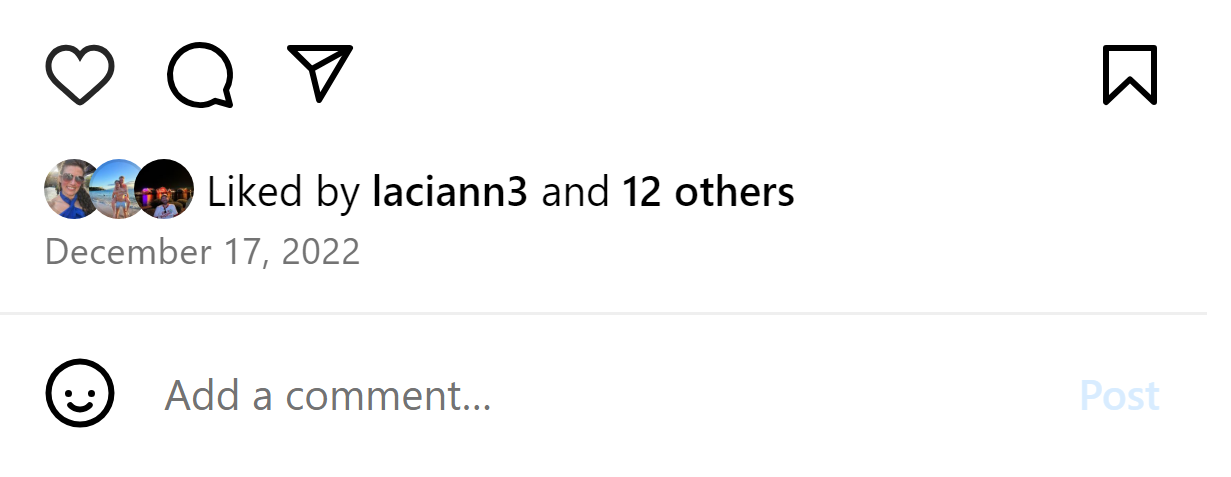
\includegraphics[width=1\textwidth,height=\textheight]{images/instagram_kpi-01.PNG}
\caption{\textbf{Instagram KPIs} (Source: @APLeithTV)}
\end{figure}

\hypertarget{customizing-kpis}{%
\subsubsection*{Customizing KPIs}\label{customizing-kpis}}
\addcontentsline{toc}{subsubsection}{Customizing KPIs}

It's also important to recognize that not all KPIs are one-size-fits-all. Customization of KPIs based on the unique nature and objectives of your business or campaign is crucial. This means taking into account factors like your industry, target audience, and the specific nuances of your brand or campaign. Customizing KPIs ensures that they are not just generic metrics, but meaningful indicators that provide real insights into the performance of your social media strategies. Tailoring these KPIs to your specific context will allow you to gather more relevant data, offering clearer insights and more actionable results.

The identification of relevant KPIs is a process that requires careful consideration of your social media goals, an understanding of common KPIs related to these goals, and the customization of these KPIs to fit the unique context of your business or campaign. By aligning KPIs with specific objectives and ensuring they are tailored to provide valuable insights, you can effectively measure the success of your social media strategies and make informed decisions to optimize your online presence.

\hypertarget{kpis-across-different-platforms}{%
\subsection*{KPIs Across Different Platforms}\label{kpis-across-different-platforms}}
\addcontentsline{toc}{subsection}{KPIs Across Different Platforms}

When delving into social media analytics, it becomes evident that each platform has its own set of dynamics and features that influence the choice and interpretation of Key Performance Indicators (KPIs). Understanding how these KPIs vary across different social media platforms is essential for accurately measuring and optimizing the impact of social media strategies.

\hypertarget{platform-specific-kpis}{%
\subsubsection*{Platform-Specific KPIs}\label{platform-specific-kpis}}
\addcontentsline{toc}{subsubsection}{Platform-Specific KPIs}

The selection of KPIs should be tailored to the specific characteristics and user engagement patterns of each platform. For example, on Facebook, `Shares' are a significant metric, indicating not only engagement but also the extent to which content resonates with users to the point of sharing it with their own networks. Similarly, Twitter's `Retweets' and `Mentions' are crucial KPIs, reflecting the spread and conversation around a piece of content. On Instagram, `Likes' and `Story Views' are key metrics, the former being a quick measure of content approval and the latter providing insight into the engagement with more temporary, day-to-day content. YouTube, with its focus on video content, places importance on `Watch Time' -- the total duration for which viewers have watched a video -- and subscriber growth, both indicative of the content's ability to attract and retain viewers over time.

\textbf{\emph{Twitch Chat Data}}

\begin{longtable}[]{@{}
  >{\raggedright\arraybackslash}p{(\columnwidth - 4\tabcolsep) * \real{0.1807}}
  >{\raggedright\arraybackslash}p{(\columnwidth - 4\tabcolsep) * \real{0.6024}}
  >{\raggedright\arraybackslash}p{(\columnwidth - 4\tabcolsep) * \real{0.2048}}@{}}
\toprule\noalign{}
\endhead
\bottomrule\noalign{}
\endlastfoot
\textbf{Variable} & \textbf{Description} & \textbf{Example} \\
id & Unique number given to each message. & 2573365 \\
channel & Name of channel in which message was sent. & \#lilypichu \\
sender & User who sent the message. & hunterlucian10 \\
message & Text of the message. & cmonBruh why \\
date & Date and time of chat message in Unix Timestamp & 1542607107593 \\
\end{longtable}

\emph{Note.} Pulled from the Twitch stream of Lilypichu on Nov 19, 2018.

\textbf{\emph{Twitch Stream Data}}

\begin{longtable}[]{@{}
  >{\raggedright\arraybackslash}p{(\columnwidth - 4\tabcolsep) * \real{0.1829}}
  >{\raggedright\arraybackslash}p{(\columnwidth - 4\tabcolsep) * \real{0.6098}}
  >{\raggedright\arraybackslash}p{(\columnwidth - 4\tabcolsep) * \real{0.1951}}@{}}
\toprule\noalign{}
\endhead
\bottomrule\noalign{}
\endlastfoot
\textbf{Variable} & \textbf{Description} & \textbf{Example} \\
id & Unique number given to each data pull. & 214439 \\
channel & Name of channel. & lilypichu \\
title & User who sent the message. & hello \\
game & Text of the message. & Just Chatting \\
viewers & Date and time of chat message in Unix Timestamp & 3607 \\
date & Date and time of data pull in Unix Timestamp & 1542754203847 \\
\end{longtable}

\emph{Note.} Pulled from the Twitch stream of Lilypichu on Nov 19, 2018.

\textbf{Twitter Data}

\begin{longtable}[]{@{}
  >{\raggedright\arraybackslash}p{(\columnwidth - 4\tabcolsep) * \real{0.1411}}
  >{\raggedright\arraybackslash}p{(\columnwidth - 4\tabcolsep) * \real{0.5031}}
  >{\raggedright\arraybackslash}p{(\columnwidth - 4\tabcolsep) * \real{0.3497}}@{}}
\toprule\noalign{}
\endhead
\bottomrule\noalign{}
\endlastfoot
\textbf{Variable} & \textbf{Description} & \textbf{Example} \\
tweet\_id & Unique numerical identifier for tweet. & 1494166530250010000 \\
user\_username & Twitter username of tweeter. & RubberNinja \\
text & Text of tweet. & @VRChat This is so cool! \\
in\_reply\_to\_user\_id & Numerical identifier of user who posted the tweet to which this is was a reply. & 2850482629 \\
lang & Language of tweet (abbreviated) & en \\
created\_at & Time tweet was posted (UTC) & 2022-02-17T04:27:15.000Z \\
author\_id & Unique numerical ID of tweeter. & 21076522 \\
conversation\_id & Unique numerical identifier of initial tweet in chain of tweets. & 1494152498617240000 \\
user\_location & Stated location of tweeter. & Los Angeles, CA \\
user\_name & Publicly displayed name of tweet poster. & RubberRoss \\
user\_description & Public description of tweeter. & \begin{minipage}[t]{\linewidth}\raggedright
My name is Ross O'Donovan, I draw and animate.\\
\url{https://t.co/05k3slkeDB} \textbar{} \url{https://t.co/EQro7JqnCD}\strut
\end{minipage} \\
user\_verified & Poster's verification status (Logical) & FALSE \\
retweet\_count & Number of retweets on this tweet. & 0 \\
like\_count & Number of likes on this tweet. & 70 \\
quote\_count & Number of quote tweets on this tweet. & 0 \\
user\_tweet\_count & Number of tweets posted by tweeter. & 31010 \\
user\_followers\_count & Number of followers of tweeter. & 689996 \\
user\_following\_count & Number of users that the tweeter follows. & 3803 \\
\end{longtable}

\emph{Note.} Not all available data is listed.

\hypertarget{understanding-platform-dynamics}{%
\subsubsection*{Understanding Platform Dynamics}\label{understanding-platform-dynamics}}
\addcontentsline{toc}{subsubsection}{Understanding Platform Dynamics}

Grasping the unique dynamics of each platform is vital in selecting and interpreting KPIs. These dynamics are shaped by the platform's design, user base, and typical content formats. For instance, YouTube's emphasis on video content means that KPIs related to view duration, such as average watch time, are particularly relevant. These metrics provide insights into viewer engagement and content quality. Similarly, on a platform like LinkedIn, where the focus is on professional networking and industry content, KPIs like `Profile Views' and `Connections' might take precedence, reflecting professional reach and network building.

This platform-specific approach to KPIs requires a deep understanding not only of the technical aspects of each platform but also of the behavioral patterns of their user bases. For example, high `Shares' on Facebook might indicate a successful content strategy that encourages community engagement and discussion, while a high number of `Retweets' on Twitter could signify the content's relevance to current trends or public discourse.

A nuanced approach to KPIs that considers the unique features and user engagement patterns of each social media platform is crucial. Such an approach allows for a more accurate and effective measurement of social media strategies, ensuring that the KPIs chosen are truly reflective of the platform's dynamics and can provide actionable insights into content performance and audience engagement.

\hypertarget{setting-and-benchmarking-kpis}{%
\subsection*{Setting and Benchmarking KPIs}\label{setting-and-benchmarking-kpis}}
\addcontentsline{toc}{subsection}{Setting and Benchmarking KPIs}

In the strategic realm of social media analytics, the process of setting and benchmarking Key Performance Indicators (KPIs) is vital for the success and relevance of social media efforts. This process ensures that the goals set are not only ambitious but also attainable, and grounded in a realistic understanding of the industry and the organization's capabilities.

\hypertarget{setting-realistic-kpis}{%
\subsubsection*{Setting Realistic KPIs}\label{setting-realistic-kpis}}
\addcontentsline{toc}{subsubsection}{Setting Realistic KPIs}

Setting realistic KPIs is a critical step in developing an effective social media strategy. This requires a careful assessment of several factors to ensure that the KPIs are not only challenging but also achievable. One of the key considerations is the current industry standards, which provide a benchmark for what is achievable and what constitutes success within a particular sector. Additionally, historical data from previous campaigns offers invaluable insights into what has been accomplished in the past and under what circumstances. This historical perspective can guide the setting of future KPIs by highlighting achievable targets based on past performance. Another important factor is the evaluation of the specific resources available, including budget, tools, and human resources, which can directly impact the feasibility of achieving certain KPIs.

\hypertarget{benchmarking-against-industry-standards}{%
\subsubsection*{Benchmarking Against Industry Standards}\label{benchmarking-against-industry-standards}}
\addcontentsline{toc}{subsubsection}{Benchmarking Against Industry Standards}

Benchmarking KPIs against industry standards and competitors is an essential practice in social media analytics. This involves an in-depth analysis of industry reports, competitor data, and leveraging tools that provide benchmarking data. By comparing an organization's KPIs with those of its peers and competitors, businesses can gain a clear understanding of where they stand in the industry landscape. This comparison can reveal strengths to be leveraged and weaknesses that need addressing, providing a roadmap for improvement and strategic adjustments. Benchmarking against industry standards also ensures that an organization's social media strategies are aligned with market realities and are competitive.

\hypertarget{regular-review-and-adjustment}{%
\subsubsection*{Regular Review and Adjustment}\label{regular-review-and-adjustment}}
\addcontentsline{toc}{subsubsection}{Regular Review and Adjustment}

The digital landscape, especially social media, is characterized by rapid changes and evolving trends. Therefore, it is essential to regularly review and adjust KPIs to align with these changes. This process involves regularly analyzing campaign performance, monitoring emerging trends in social media, and revising business objectives as needed. Regular review ensures that KPIs remain relevant and aligned with the current social media environment and business goals. Adjustments may involve redefining target metrics, shifting focus to different platforms, or revising strategies to better engage with the audience. This dynamic approach to KPI management is crucial for maintaining the effectiveness and relevance of social media strategies in an ever-changing digital landscape.

Setting realistic KPIs, benchmarking them against industry standards, and regularly reviewing and adjusting these indicators are fundamental practices in social media analytics. These processes ensure that social media efforts are strategically aligned, competitively positioned, and agile enough to adapt to the fast-paced nature of social media trends and market dynamics.

\hypertarget{measuring-engagement-reach-and-influence}{%
\section*{Measuring Engagement, Reach, and Influence}\label{measuring-engagement-reach-and-influence}}
\addcontentsline{toc}{section}{Measuring Engagement, Reach, and Influence}

In the intricate world of social media, understanding and accurately measuring key metrics like engagement, reach, and influence is essential for gauging the effectiveness of social media strategies. These metrics offer profound insights into audience interactions, the spread of content, and its overall impact. This section explores the nuances of these metrics, including their definitions, measurement tools and techniques, and the methodologies for their effective interpretation and analysis.

Engagement on social media is a measure of how users interact with content. It encompasses actions such as likes, comments, shares, and views. Engagement metrics are critical as they indicate not only the popularity of the content but also the extent to which it resonates with the audience. High engagement rates often suggest that the content is relevant, appealing, and provokes a reaction from the audience. To measure engagement, one can use native analytic tools provided by the social media platforms themselves, such as Facebook Insights or Instagram Analytics. These tools track the number of interactions and provide detailed breakdowns of engagement types.

Reach, another pivotal metric, refers to the total number of unique users who have seen a piece of content. Unlike engagement, which focuses on interactions, reach provides insights into the visibility and extent of content dissemination. It's a crucial metric for understanding the potential audience size and measuring brand awareness. Reach can be measured through the same native analytics tools, which provide data on how many users have seen a post or campaign. Understanding reach helps in assessing the effectiveness of content distribution strategies and the platform's algorithm in content promotion.

Influence, while more nuanced, is about the capacity of the content or the social media presence to affect audience behavior or opinions. Influence can be reflected in various forms, such as the growth in follower count, the extent to which content is shared beyond the immediate audience, and conversions or actions taken as a result of the content. Measuring influence often involves a combination of quantitative data (like follower growth rate and share metrics) and qualitative insights (like audience feedback and sentiment analysis). Tools for measuring influence include both platform-specific analytics and third-party tools that offer deeper insights into audience behavior and content impact.

Effectively measuring and analyzing these metrics requires a blend of using the right tools, understanding the nuances of each metric, and aligning them with the objectives of the social media strategy. For instance, a campaign focused on brand awareness would prioritize reach and influence, while one aimed at community building would look closely at engagement metrics. The key is to interpret these metrics in the context of specific goals and the overarching social media strategy.

Engagement, reach, and influence are indispensable metrics in social media analytics. Accurately measuring and analyzing these metrics provide valuable insights into how content performs, how it resonates with audiences, and the overall impact of social media efforts. This understanding is crucial for crafting effective strategies, optimizing content, and achieving desired outcomes in the competitive landscape of social media.

\hypertarget{defining-reach-engagement-and-influence}{%
\subsection*{Defining Reach, Engagement, and Influence}\label{defining-reach-engagement-and-influence}}
\addcontentsline{toc}{subsection}{Defining Reach, Engagement, and Influence}

In the field of social media analytics, three key metrics stand out as essential gauges of content and campaign success: engagement, reach, and influence. Each of these metrics offers distinct insights into how users interact with and respond to social media content, and they are pivotal in shaping effective social media strategies.

\hypertarget{reach}{%
\subsubsection*{Reach}\label{reach}}
\addcontentsline{toc}{subsubsection}{Reach}

Reach refers to the total number of unique users who have seen a particular piece of content on social media. It is a vital metric for measuring the visibility and extent of content dissemination. Unlike engagement, which focuses on the depth of interaction with the content, reach is about the breadth of content exposure. It offers insights into the scale at which content is being seen and is crucial for campaigns focusing on brand awareness and exposure. Reach can be affected by various factors, including the platform's algorithm, the timing of the post, and the inherent appeal of the content. Understanding reach is fundamental for strategists looking to maximize their content's visibility across the social media landscape.

\hypertarget{engagement}{%
\subsubsection*{Engagement}\label{engagement}}
\addcontentsline{toc}{subsubsection}{Engagement}

Engagement on social media is a comprehensive term that encompasses how users interact with content. This interaction can take various forms, such as likes, comments, shares, and views. Likes indicate a basic level of user approval or interest, comments reflect a deeper level of engagement with the potential for dialogue, shares signify the content's appeal to the extent that users want to disseminate it within their networks, and views are essential for understanding the overall reach and impact, especially of video content. Engagement metrics are critical because they provide a direct indicator of how compelling, relevant, and resonant the content is with the audience. High engagement rates are often correlated with content that effectively captures and retains the audience's attention, sparking interest, and encouraging interaction.

\begin{figure}
\centering

\includegraphics[width=1\textwidth,height=\textheight]{images/engagement.jpg}
\caption{\textbf{Social Media Engagement} (Source: The Brandon Agency)}
\end{figure}

\hypertarget{influence}{%
\subsubsection*{Influence}\label{influence}}
\addcontentsline{toc}{subsubsection}{Influence}

Influence in social media pertains to the capacity of content or an account to affect the behavior or opinions of the audience. This metric is closely linked to the credibility and authority of the content creator or brand. Influence can be seen in various forms, such as the growth in follower count, indicating an increasing audience base; the virality of content, where the content spreads rapidly and widely across platforms; and conversions, where the content leads to specific user actions like website visits, sign-ups, or purchases. Influence is a nuanced metric that combines the elements of reach and engagement to reflect the overall impact and persuasive power of social media content.

Understanding reach, engagement, and influence is fundamental for anyone engaged in social media analytics. These metrics provide a comprehensive picture of how content is performing, how far it is reaching, and the extent of its impact on the audience. They are critical tools for assessing the effectiveness of social media strategies and guiding decisions to optimize content for maximum engagement and influence.

\hypertarget{techniques-and-tools-for-measurement}{%
\subsection*{Techniques and Tools for Measurement}\label{techniques-and-tools-for-measurement}}
\addcontentsline{toc}{subsection}{Techniques and Tools for Measurement}

In the realm of social media analytics, the selection and use of appropriate tools and techniques for measuring key metrics like engagement, reach, and influence are essential. These tools range from native analytics provided by social media platforms to sophisticated third-party analytical tools, each offering distinct features and capabilities. Understanding these tools and selecting the right ones based on specific needs and goals are crucial steps in effective social media analytics.

\hypertarget{analytical-tools-introduction}{%
\subsubsection*{Analytical Tools Introduction}\label{analytical-tools-introduction}}
\addcontentsline{toc}{subsubsection}{Analytical Tools Introduction}

Each major social media platform offers its own set of native analytics tools, designed to provide insights into the performance of content and campaigns on their respective platforms. Facebook Insights, for instance, offers in-depth data on page performance, audience demographics, and engagement metrics. Twitter Analytics provides valuable insights into tweet performance, audience interests, and engagement trends. Instagram Insights delivers data on follower demographics, post performance, and stories analytics. LinkedIn Analytics, on the other hand, focuses on professional audience engagement, content reach, and page growth metrics. These native tools are essential for any social media strategy as they provide specific data directly from the source, enabling a clear understanding of how content performs on each platform.

\hypertarget{third-party-analytical-tools}{%
\subsubsection*{Third-Party Analytical Tools}\label{third-party-analytical-tools}}
\addcontentsline{toc}{subsubsection}{Third-Party Analytical Tools}

In addition to native analytics, there are numerous third-party tools available that offer more advanced analytics and integrated insights across multiple platforms. Tools like Hootsuite, Google Analytics, and Sprout Social are widely used in the industry. Hootsuite, for example, allows for comprehensive monitoring and management of multiple social media accounts in one place, offering analytics that helps track key metrics, schedule posts, and engage with audiences. Google Analytics is instrumental in tracking website traffic from social media platforms, providing insights into user behavior, conversions, and the effectiveness of social media campaigns in driving web traffic. Sprout Social offers detailed analytics, social listening, and engagement tools, helping businesses to understand and interact with their audience more effectively. These third-party tools are valuable for their ability to consolidate data from various sources and provide a more holistic view of social media performance.

\begin{figure}
\centering
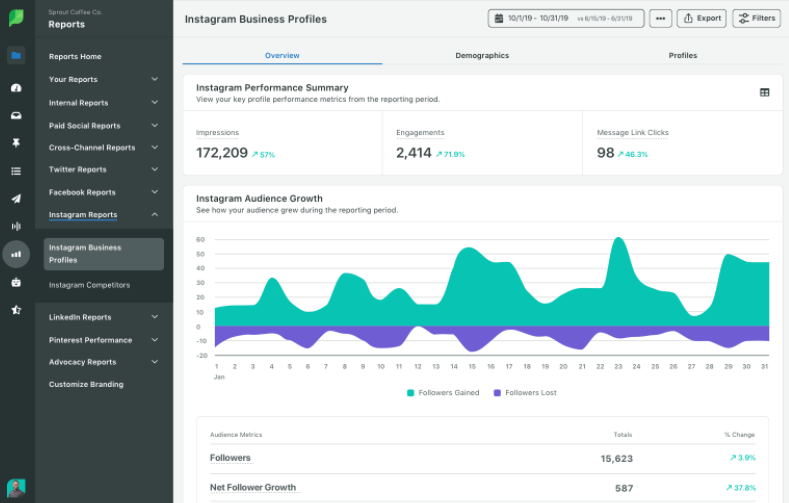
\includegraphics[width=1\textwidth,height=\textheight]{images/sprout.png}
\caption{\textbf{Sprout Social} (Source: Digital Marketer's World)}
\end{figure}

\hypertarget{tool-selection-criteria}{%
\subsubsection*{Tool Selection Criteria}\label{tool-selection-criteria}}
\addcontentsline{toc}{subsubsection}{Tool Selection Criteria}

When selecting the most appropriate tools for social media measurement, several criteria need to be considered. Platform coverage is essential; the tool should support analytics for all the platforms used in your social media strategy. The depth of analytics is another critical factor - the tool should provide detailed insights that go beyond basic metrics to include audience analysis, competitor analysis, and trend tracking. Real-time tracking capabilities are also crucial for monitoring ongoing campaigns and responding promptly to engagement opportunities. Finally, the ease of use and user interface of the tool should be considered to ensure efficiency and usability for all team members.

A comprehensive understanding and careful selection of analytical tools are fundamental for effective social media measurement. By leveraging the strengths of both native and third-party tools and choosing them based on specific criteria, social media professionals can gain deep insights, drive strategy, and optimize their social media presence effectively.

\hypertarget{engagement-metrics-and-their-interpretation}{%
\subsection*{Engagement Metrics and Their Interpretation}\label{engagement-metrics-and-their-interpretation}}
\addcontentsline{toc}{subsection}{Engagement Metrics and Their Interpretation}

In the landscape of social media, understanding and interpreting engagement metrics is vital for assessing how users interact with content. These metrics offer insights into the effectiveness of social media strategies, user behavior, and content performance. This section delves into the various types of engagement metrics, the techniques for measuring them, and the methodologies for interpreting this data to inform future strategies.

\hypertarget{types-of-engagement-metrics}{%
\subsubsection*{Types of Engagement Metrics}\label{types-of-engagement-metrics}}
\addcontentsline{toc}{subsubsection}{Types of Engagement Metrics}

Engagement metrics in social media encompass a range of indicators that show how users are interacting with content. Likes, for example, are a basic yet powerful metric indicating user approval or interest. Comment rates go a step further, showing not just interest but active engagement and willingness to participate in a conversation or express opinions. Share counts are particularly significant, as they indicate that the content resonated strongly enough with users that they chose to spread it within their own networks. Finally, video view statistics are essential in the age of digital media, providing insights into how long users are engaging with video content, which is increasingly becoming the most consumed type of content online. Each of these metrics offers specific insights into user interaction and is crucial for evaluating the success of social media content.

\hypertarget{measurement-techniques}{%
\subsubsection*{Measurement Techniques}\label{measurement-techniques}}
\addcontentsline{toc}{subsubsection}{Measurement Techniques}

To effectively measure these engagement metrics, one must utilize the tools and techniques available through both native and third-party analytics platforms. Tracking engagement trends over time allows for an understanding of how engagement evolves in response to different content strategies or external factors. Comparing engagement across different content types can highlight what resonates best with your audience, whether it be text posts, images, or videos. Understanding peak engagement times is also crucial; it involves analyzing when your audience is most active on the platform, which can greatly impact the visibility and engagement of your posts. Regularly monitoring these metrics enables a dynamic approach to content strategy, allowing for adjustments and optimizations based on real-time feedback and trends.

\hypertarget{interpreting-engagement-data}{%
\subsubsection*{Interpreting Engagement Data}\label{interpreting-engagement-data}}
\addcontentsline{toc}{subsubsection}{Interpreting Engagement Data}

The interpretation of engagement data is where the real analytical skill comes into play. High engagement rates might indicate that your content is highly relevant and appealing to your audience, but it's important to dive deeper. Understanding what different levels and types of engagement indicate about your content's performance is crucial. For instance, a high number of likes but few comments might suggest that while the content is well-received, it may not be provocative or engaging enough to spark a conversation. Analyzing comment sentiment can provide insights into audience preferences and content relevance. Similarly, understanding the context behind share counts can offer clues about the content's ability to generate interest or controversy. Interpreting these metrics in the context of your overall content strategy, audience demographics, and platform trends is key to gaining actionable insights that can drive more effective social media strategies.

Engagement metrics are fundamental to understanding how users interact with social media content. By effectively measuring and interpreting these metrics, social media professionals can gain a deeper understanding of their audience, refine their content strategies, and enhance their overall social media presence. This process involves not just the collection of data but also its careful analysis to draw meaningful insights that can inform future strategies.

\hypertarget{reach-and-influence-analysis}{%
\subsection*{Reach and Influence Analysis}\label{reach-and-influence-analysis}}
\addcontentsline{toc}{subsection}{Reach and Influence Analysis}

In the domain of social media analytics, understanding and analyzing reach and influence is crucial for evaluating the effectiveness of content and campaigns. Reach refers to the extent to which content is seen by users, while influence pertains to the content's ability to affect user behavior or opinions. This section explores the methodologies for calculating reach, measuring influence, and includes case studies to illustrate successful strategies in these areas.

\hypertarget{calculating-reach}{%
\subsubsection*{Calculating Reach}\label{calculating-reach}}
\addcontentsline{toc}{subsubsection}{Calculating Reach}

Reach on social media can be broadly categorized into organic reach and paid reach. Organic reach refers to the number of unique users who see your content without paid promotion. It is influenced by various factors such as the content's relevance, the time of posting, and the platform's algorithm. Organic reach is often seen as a measure of the natural appeal and quality of the content. On the other hand, paid reach involves using paid advertising to increase the visibility of content. It can be targeted based on specific demographics, interests, and behaviors, and is often used to boost exposure to new or wider audiences. Understanding these different types of reach and the factors that influence them is essential for developing strategies to maximize the visibility of social media content.

\hypertarget{influence-measurement}{%
\subsubsection*{Influence Measurement}\label{influence-measurement}}
\addcontentsline{toc}{subsubsection}{Influence Measurement}

Measuring the influence of social media content and campaigns involves assessing the impact on audience behavior and opinions. This can be gauged through various metrics, such as the level of engagement (likes, comments, shares), the growth in follower count, and the extent of content virality. The role of influencers -- individuals with significant followings and the ability to sway their audience -- is also critical in influence measurement. Influencer partnerships can amplify a campaign's reach and impact. Additionally, the significance of user-generated content in driving engagement and fostering community participation is another aspect of measuring influence. Moreover, conversions resulting from social media interactions, such as website visits, sign-ups, or purchases, are tangible indicators of the campaign's influence on user behavior.

\hypertarget{interpreting-metrics-for-strategic-insights}{%
\section*{Interpreting Metrics for Strategic Insights}\label{interpreting-metrics-for-strategic-insights}}
\addcontentsline{toc}{section}{Interpreting Metrics for Strategic Insights}

\hypertarget{interpreting-metrics-for-strategic-insights-1}{%
\section{Interpreting Metrics for Strategic Insights}\label{interpreting-metrics-for-strategic-insights-1}}

In the constantly evolving digital landscape, the ability to effectively interpret and utilize social media metrics for strategic insights is indispensable. Social media platforms generate a vast amount of raw data, but the real value lies in transforming this data into actionable insights that can guide business strategies and decisions. This crucial aspect of social media analytics involves not only understanding what the data represents but also how it can be applied to meet business objectives. This section delves into the methodologies for analyzing social media metrics, supplemented with case studies for practical application, and highlights the importance of continuous monitoring and adaptation of strategies based on these insights.

Firstly, interpreting metrics requires a deep understanding of what each metric represents and its relevance to specific business goals. For example, a high number of likes or shares may indicate content popularity, but it's essential to analyze further to understand the implications for brand awareness or customer engagement. Engagement rates, click-through rates, and conversion rates are often more telling metrics, providing deeper insights into audience behavior and the effectiveness of content strategies.

The analysis of these metrics should be methodical and aligned with the business's overall objectives. For instance, if the goal is to increase brand awareness, analyzing reach and impressions will be more relevant. If the aim is to drive sales, then conversion rates and click-through rates will be key metrics to focus on. This targeted analysis helps in making informed decisions about content strategy, marketing campaigns, and audience engagement tactics.

Case studies serve as valuable tools for understanding the practical application of these metrics. They provide real-world examples of how businesses have successfully leveraged social media metrics to achieve their objectives, or how a misinterpretation of these metrics led to less than favorable outcomes. Learning from these case studies, both successes and failures, can provide critical insights and guide strategy formulation.

The dynamic nature of social media means that continuous monitoring and adjustment of strategies are essential. Social media trends, platform algorithms, and audience preferences can change rapidly. Regular analysis of KPIs and other metrics allows businesses to stay agile, making necessary adjustments to their strategies in real-time. This might involve shifting focus between different platforms, altering content types, or modifying engagement tactics based on the latest data.

Interpreting social media metrics for strategic insights is a multifaceted process that involves understanding each metric's significance, aligning them with business goals, learning from practical examples, and continually adapting strategies based on ongoing analysis. This approach ensures that businesses can not only track the performance of their social media efforts but also gain valuable insights that drive growth and improvement in their digital marketing strategies.

\hypertarget{translating-metrics-into-actionable-insights}{%
\subsection*{Translating Metrics into Actionable Insights}\label{translating-metrics-into-actionable-insights}}
\addcontentsline{toc}{subsection}{Translating Metrics into Actionable Insights}

In the realm of social media analytics, the ability to translate metrics into actionable insights is crucial for refining strategies and achieving desired outcomes. This process involves a comprehensive analysis of data, recognition of patterns, and the application of these insights to enhance social media planning and execution. This section explores the methodologies for data analysis, techniques for pattern recognition, and ways to turn data into effective strategy.

\hypertarget{methodologies-for-data-analysis}{%
\subsubsection*{Methodologies for Data Analysis}\label{methodologies-for-data-analysis}}
\addcontentsline{toc}{subsubsection}{Methodologies for Data Analysis}

Analyzing social media data requires a robust understanding of various analytical methodologies that can uncover meaningful insights from metrics. Trend analysis is a fundamental technique that involves examining data over time to identify consistent patterns or anomalies. For example, a steady increase in engagement rates might indicate growing audience interest or the effectiveness of a particular content strategy. Comparative analysis is another critical method, allowing for the comparison of different data sets, such as engagement rates across different platforms or time periods. This analysis helps in understanding what strategies work best and where there might be room for improvement. Correlation studies involve examining the relationship between different variables, for instance, how changes in posting frequency might correlate with engagement rates. Understanding these relationships helps in identifying what factors most significantly impact campaign performance and user behavior.

\hypertarget{pattern-recognition-in-metrics}{%
\subsubsection*{Pattern Recognition in Metrics}\label{pattern-recognition-in-metrics}}
\addcontentsline{toc}{subsubsection}{Pattern Recognition in Metrics}

Recognizing patterns within social media metrics is key to identifying both opportunities and potential issues. This involves a detailed examination of metrics to detect shifts in user engagement, content performance, and audience demographics. For instance, a sudden spike in engagement on specific types of posts can reveal emerging content preferences of the audience. Similarly, changes in audience demographics, such as a shift in the age or geographical location of the majority of followers, can indicate evolving audience dynamics and help in tailoring content accordingly. Recognizing these patterns enables social media analysts to anticipate trends, adapt strategies, and address any emerging issues proactively.

\hypertarget{turning-data-into-strategy}{%
\subsubsection*{Turning Data into Strategy}\label{turning-data-into-strategy}}
\addcontentsline{toc}{subsubsection}{Turning Data into Strategy}

The ultimate goal of analyzing social media metrics is to turn these insights into an effective strategy. Data-driven insights can significantly inform content strategy, helping determine what type of content resonates most with the audience, the ideal posting schedule, and the most effective content formats. Audience targeting can also be refined based on demographic insights and user behavior patterns, ensuring that content reaches and engages the most relevant audience. Overall social media planning benefits from these insights, as they guide decision-making in content creation, platform selection, and engagement tactics. By integrating these insights into the planning process, social media strategies can become more focused, responsive, and effective in achieving their objectives.

Translating metrics into actionable insights involves a comprehensive analysis of social media data, recognition of important patterns, and the application of these insights to refine and enhance social media strategies. This process is crucial for navigating the dynamic landscape of social media and for ensuring that social media efforts are strategically aligned and capable of achieving desired results.

\hypertarget{aligning-metrics-with-business-objectives}{%
\subsection*{Aligning Metrics with Business Objectives}\label{aligning-metrics-with-business-objectives}}
\addcontentsline{toc}{subsection}{Aligning Metrics with Business Objectives}

In the strategic practice of social media analytics, aligning metrics with business objectives is pivotal for ensuring that social media efforts contribute effectively to overarching goals. This section emphasizes the importance of this alignment and offers guidance on adjusting strategies based on metric analysis to optimize performance.

\hypertarget{importance-of-alignment}{%
\subsubsection*{Importance of Alignment}\label{importance-of-alignment}}
\addcontentsline{toc}{subsubsection}{Importance of Alignment}

The alignment of social media metrics with business or campaign objectives is critical for the success of any digital marketing effort. Social media metrics should not be viewed in isolation but rather as indicators that inform and reflect the broader business goals. For instance, if the objective is to enhance brand awareness, metrics like reach, impressions, and follower growth rate are particularly relevant as they provide insights into the brand's visibility and recognition. For objectives such as lead generation, metrics like click-through rates and conversion rates become more crucial, as they directly relate to the effectiveness of social media in generating potential customer leads. Similarly, for goals centered around customer engagement or sales, metrics like engagement rates and direct inquiries or sales through social media channels are key indicators of success. This alignment ensures that every aspect of a social media strategy is geared towards and measured against the specific goals it aims to achieve.

\hypertarget{adjusting-strategies-based-on-metrics}{%
\subsubsection*{Adjusting Strategies Based on Metrics}\label{adjusting-strategies-based-on-metrics}}
\addcontentsline{toc}{subsubsection}{Adjusting Strategies Based on Metrics}

Analyzing social media metrics offers valuable insights that can inform the adjustment and refinement of strategies. Based on metric performance, content strategies may need to be refined. For example, if video content consistently shows higher engagement rates, the strategy might shift to include more video content. If certain types of posts are seen to drive higher conversion rates, they can be prioritized in content planning. Targeting efforts might also be adjusted based on insights into audience demographics and behaviors derived from social media metrics. If data shows that a particular demographic is more engaged or more likely to convert, targeting strategies can be honed to focus more on that segment. Engagement tactics, such as the timing of posts, frequency, and types of interactions, can also be optimized based on metrics. For example, if engagement peaks at specific times, posting schedules can be adjusted accordingly.

The alignment of social media metrics with business objectives is essential for ensuring that social media activities are focused and effective. Regular analysis of these metrics allows for strategic adjustments and optimizations, ensuring that the social media strategy remains aligned with and conducive to achieving the desired business outcomes. This ongoing process of alignment and adjustment is a critical component of successful social media analytics and strategy.

\hypertarget{continuous-monitoring-and-adjustment}{%
\subsection*{Continuous Monitoring and Adjustment}\label{continuous-monitoring-and-adjustment}}
\addcontentsline{toc}{subsection}{Continuous Monitoring and Adjustment}

In the fast-paced and ever-evolving world of social media, continuous monitoring and strategic adjustment based on analytics are essential for maintaining the relevance and effectiveness of social media strategies. This section underscores the necessity of ongoing analysis, provides recommendations for setting up regular reporting structures, and discusses the importance of strategic pivoting based on insights gleaned from social media metrics.

\hypertarget{the-need-for-ongoing-analysis}{%
\subsubsection*{The Need for Ongoing Analysis}\label{the-need-for-ongoing-analysis}}
\addcontentsline{toc}{subsubsection}{The Need for Ongoing Analysis}

Continuous monitoring of social media metrics is crucial, as the digital landscape and user behaviors are constantly changing. Relying solely on one-time analysis can lead to outdated strategies that fail to resonate with the current audience. Ongoing analysis allows for the identification of trends, shifts in audience preferences, and emerging opportunities or challenges. By consistently tracking metrics such as engagement rates, reach, follower growth, and conversion rates, businesses can gain a real-time understanding of their social media performance. This continuous monitoring enables timely responses to changes in the social media environment, ensuring that strategies remain aligned with current user behaviors and platform algorithms.

\hypertarget{recommendations-for-regular-reporting}{%
\subsubsection*{Recommendations for Regular Reporting}\label{recommendations-for-regular-reporting}}
\addcontentsline{toc}{subsubsection}{Recommendations for Regular Reporting}

To effectively implement continuous monitoring, it is recommended to establish regular reporting structures. These can take the form of weekly or monthly performance reviews, depending on the scale and dynamics of the social media activities. Regular reporting should encompass a comprehensive analysis of key metrics, comparisons against previous periods, and benchmarking against industry standards or competitors. Utilizing dashboards and analytical tools can simplify the process, providing clear and accessible insights into performance trends. These reports should not only present data but also offer actionable insights and recommendations for strategy adjustments. Regular reporting ensures that stakeholders are kept informed and that strategic decisions are data-driven.

\hypertarget{strategic-pivoting-based-on-insights}{%
\subsubsection*{Strategic Pivoting Based on Insights}\label{strategic-pivoting-based-on-insights}}
\addcontentsline{toc}{subsubsection}{Strategic Pivoting Based on Insights}

The ability to pivot strategies based on insights from ongoing analysis is a critical aspect of agile social media management. Insights gained from continuous monitoring should inform strategic decisions, allowing businesses to adapt to the changing digital landscape swiftly. This might involve reallocating resources to more effective channels if certain platforms are underperforming, experimenting with new types of content that are resonating with the audience, or adjusting targeting criteria to better reach the desired demographic. Strategic pivoting based on real-time data allows businesses to capitalize on emerging trends, mitigate risks, and optimize the ROI of their social media efforts.

Continuous monitoring and the ability to adjust strategies based on ongoing insights are fundamental for the success of social media initiatives. By embracing a dynamic approach to social media analytics, businesses can ensure that their strategies are responsive, relevant, and effective in achieving their desired social media objectives.

\hypertarget{studying-successful-social-media-campaigns}{%
\chapter{Studying Successful Social Media Campaigns}\label{studying-successful-social-media-campaigns}}

\hypertarget{analysis-of-successful-campaigns-across-various-platforms}{%
\section*{Analysis of Successful Campaigns Across Various Platforms}\label{analysis-of-successful-campaigns-across-various-platforms}}
\addcontentsline{toc}{section}{Analysis of Successful Campaigns Across Various Platforms}

\hypertarget{case-study-selection-and-criteria}{%
\subsection*{Case Study Selection and Criteria}\label{case-study-selection-and-criteria}}
\addcontentsline{toc}{subsection}{Case Study Selection and Criteria}

\hypertarget{level-of-engagement}{%
\subsubsection*{Level of Engagement}\label{level-of-engagement}}
\addcontentsline{toc}{subsubsection}{Level of Engagement}

Engagement metrics are crucial indicators of a campaign's resonance with its audience. Metrics such as likes, shares, comments, and views offer quantifiable evidence of how users interact with and respond to social media content. High engagement rates typically suggest that the content is effective in capturing and retaining the audience's interest. Analyzing these metrics can reveal insights into the types of content that resonate most with users, optimal posting times, and the overall effectiveness of the campaign's communication strategy.

\hypertarget{achievement-of-specific-goals}{%
\subsubsection*{Achievement of Specific Goals}\label{achievement-of-specific-goals}}
\addcontentsline{toc}{subsubsection}{Achievement of Specific Goals}

The success of a campaign is also measured by how well it meets its predefined objectives. These objectives can range from increasing brand awareness and driving sales to advocating for social causes or fostering community engagement. This criterion involves evaluating the extent to which the campaign's goals were achieved and understanding the strategies that contributed to this success. For instance, a campaign aimed at driving sales would be assessed on metrics like conversion rates and revenue growth, while a campaign focused on raising awareness might be evaluated based on reach and public engagement.

\hypertarget{creativity-and-innovation}{%
\subsubsection*{Creativity and Innovation}\label{creativity-and-innovation}}
\addcontentsline{toc}{subsubsection}{Creativity and Innovation}

Creativity and innovation in campaign design and execution play a pivotal role in standing out in the crowded social media landscape. This includes novel uses of social media features, creative content strategies, and innovative engagement tactics. Campaigns that leverage these aspects effectively often achieve higher engagement and can set new trends in social media marketing. The evaluation of creativity and innovation requires not only an analysis of the campaign's content and strategies but also an understanding of the context and standards of the time when the campaign was executed.

\hypertarget{sustainability-and-long-term-impact}{%
\subsubsection*{Sustainability and Long-term Impact}\label{sustainability-and-long-term-impact}}
\addcontentsline{toc}{subsubsection}{Sustainability and Long-term Impact}

The long-term impact and sustainability of a campaign are significant indicators of success. This involves looking beyond immediate metrics to understand the enduring effects on brand perception, customer loyalty, and community engagement. A campaign with a lasting impact not only achieves its immediate goals but also contributes to the long-term growth and stability of the brand or cause it represents. This criterion assesses how the campaign has influenced the target audience over time and the extent to which it has fostered ongoing engagement and support.

Selecting case studies based on these criteria will provide comprehensive insights into the various factors that contribute to the success of social media campaigns. This approach ensures a balanced analysis, encompassing both quantitative metrics and qualitative aspects of campaign execution and impact.

\hypertarget{diverse-platform-analysis}{%
\subsection*{Diverse Platform Analysis}\label{diverse-platform-analysis}}
\addcontentsline{toc}{subsection}{Diverse Platform Analysis}

In the chapter ``Studying Successful Social Media Campaigns,'' it is essential to explore how different social media platforms contribute to the success of various campaigns. Each platform has unique features and caters to specific audience demographics, making an understanding of these distinctions crucial for effective campaign planning and analysis. This section delves into how successful campaigns have utilized the distinct characteristics of various platforms to maximize their impact.

\hypertarget{facebook}{%
\subsubsection*{Facebook}\label{facebook}}
\addcontentsline{toc}{subsubsection}{Facebook}

Facebook, known for its broad demographic reach and sophisticated targeting options, allows campaigns to connect with a diverse audience. Dove's ``Real Beauty Sketches'' campaign effectively utilized Facebook to promote its message of body positivity and self-esteem. By leveraging Facebook's targeting capabilities, the campaign could reach a wide range of demographics, resonating with a diverse audience and sparking meaningful conversations about beauty standards.

\begin{figure}
\centering
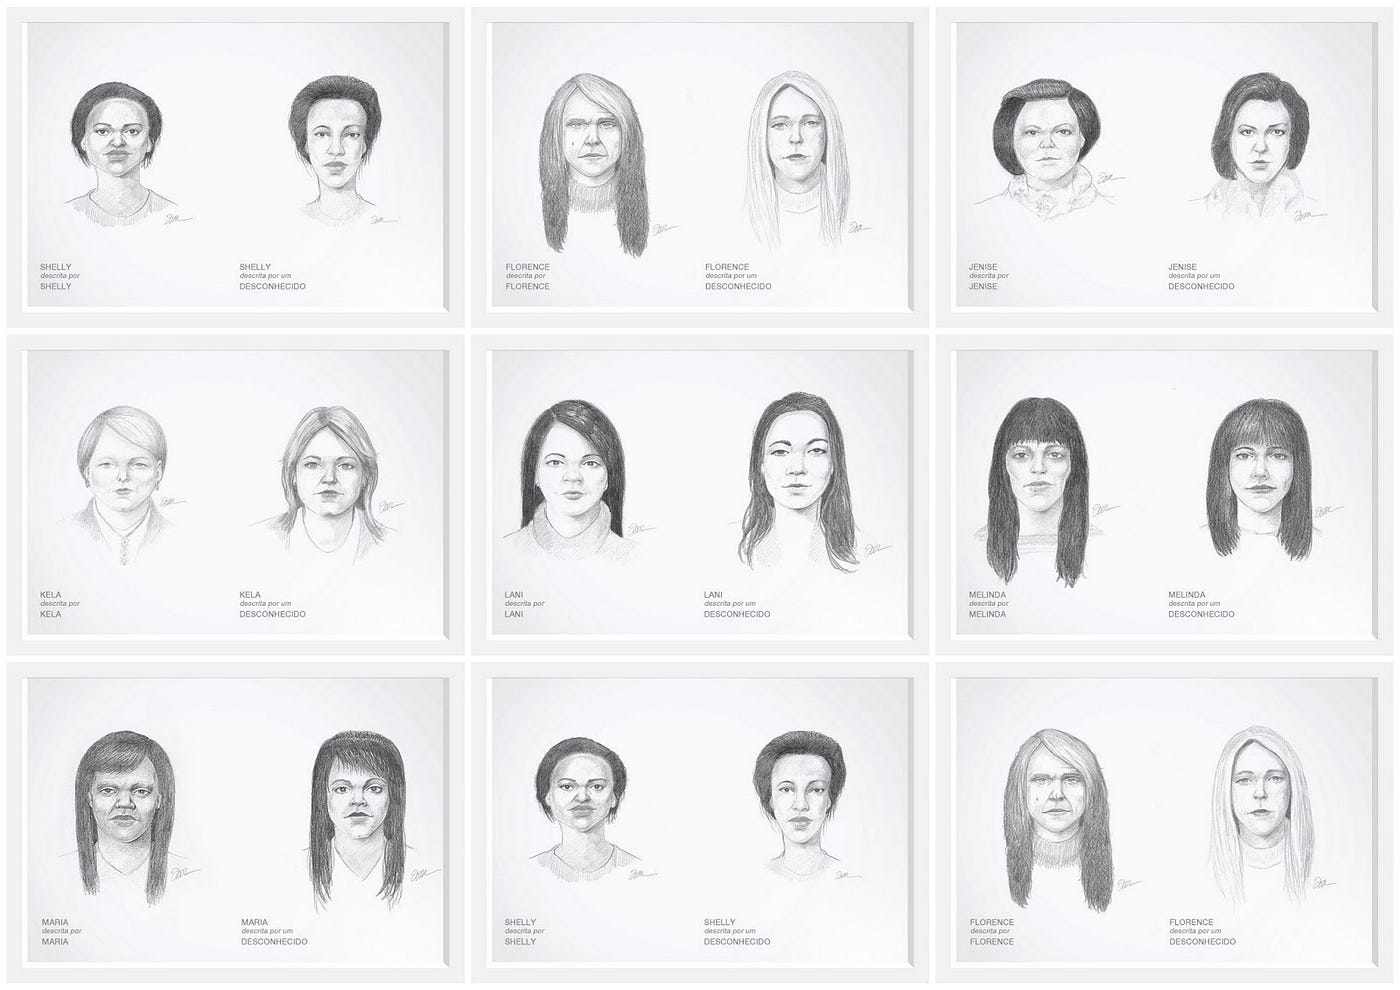
\includegraphics[width=1\textwidth,height=\textheight]{images/dove.jpg}
\caption{Dove: Real Beauty Sketches}
\end{figure}

\hypertarget{twitter}{%
\subsubsection*{Twitter}\label{twitter}}
\addcontentsline{toc}{subsubsection}{Twitter}

Twitter excels in facilitating real-time communication and the widespread use of hashtags, making it ideal for engaging campaigns and viral content. The ``\#NuggsForCarter'' campaign by Wendy's demonstrated Twitter's power in driving viral content. The campaign's clever use of a personal challenge, combined with a strategic hashtag, led to record-breaking engagement and elevated brand visibility.

\begin{figure}
\centering
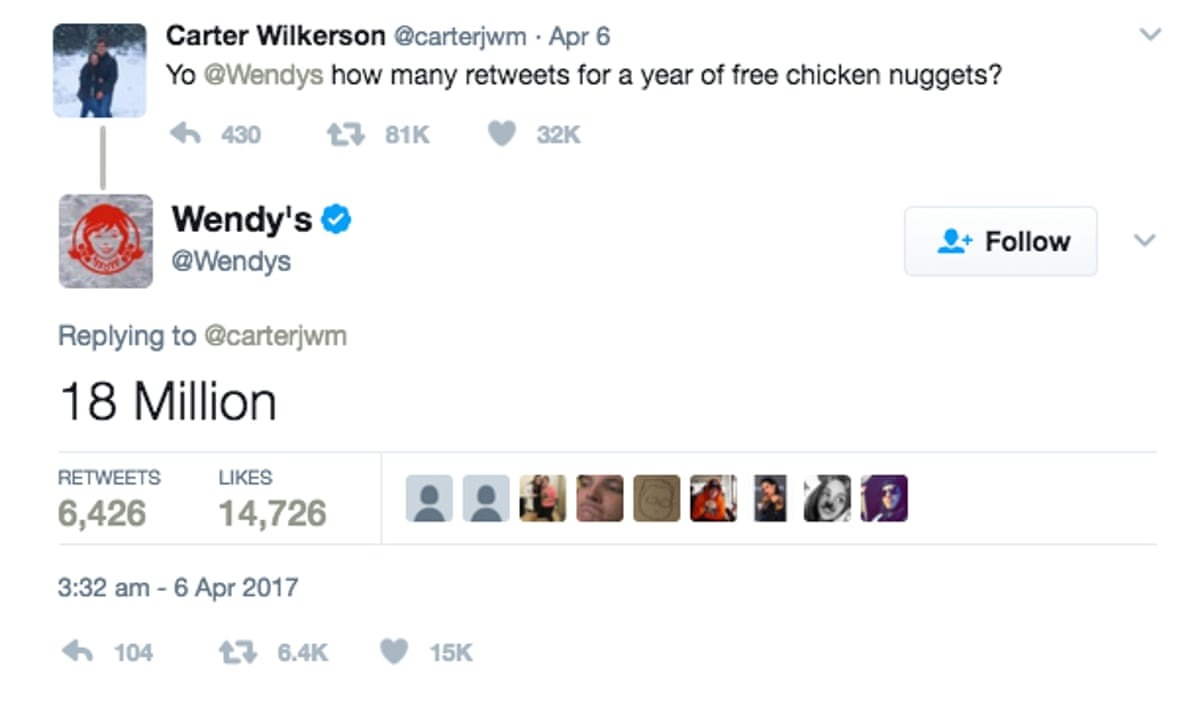
\includegraphics[width=1\textwidth,height=\textheight]{images/wendys.jpg}
\caption{Wendy's \#NuggsForCarter}
\end{figure}

\hypertarget{instagram}{%
\subsubsection*{Instagram}\label{instagram}}
\addcontentsline{toc}{subsubsection}{Instagram}

Instagram's strength lies in its visual-centric approach, allowing for powerful storytelling through imagery. National Geographic's use of Instagram exemplifies effective storytelling through captivating visuals. Their posts, which often feature stunning photography and engaging narratives, attract a vast audience interested in travel, nature, and culture.

\begin{figure}
\centering
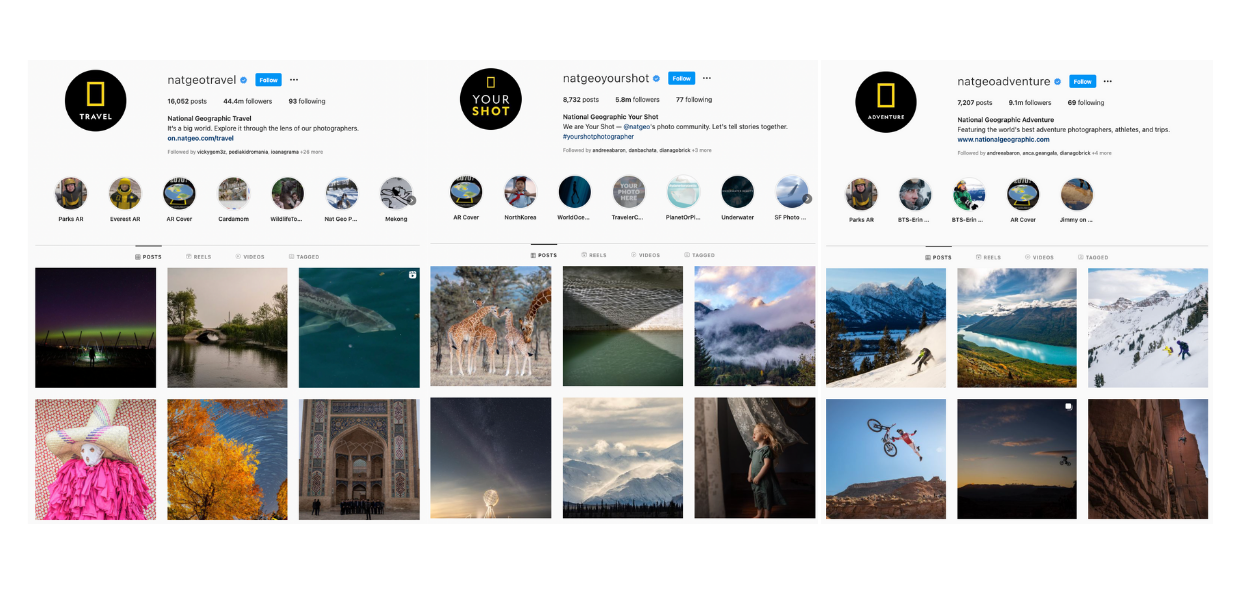
\includegraphics[width=1\textwidth,height=\textheight]{images/natgeo.png}
\caption{National Geographic: Themed Accounts}
\end{figure}

\hypertarget{linkedin}{%
\subsubsection*{LinkedIn}\label{linkedin}}
\addcontentsline{toc}{subsubsection}{LinkedIn}

LinkedIn's professional network is optimal for campaigns targeting business professionals and job seekers. Upwork's campaign on LinkedIn strategically leveraged the platform's professional user base. By showcasing a carousel of potential jobs, Upwork effectively connected with both companies seeking employees and professionals looking for opportunities, thus reinforcing its position as a leading freelancing platform.

\begin{figure}
\centering
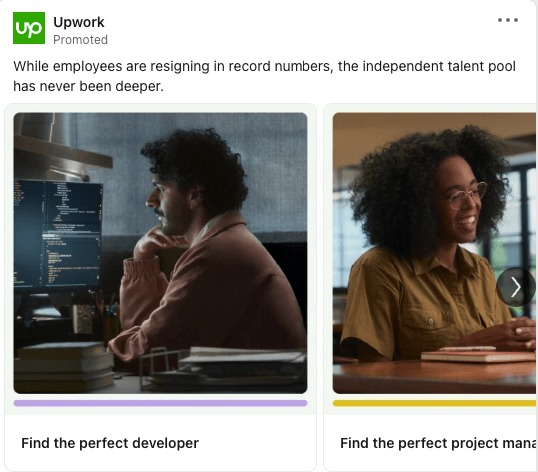
\includegraphics[width=0.75\textwidth,height=\textheight]{images/upwork.jpg}
\caption{Upwork: Assisting Job Seekers}
\end{figure}

\hypertarget{tiktok}{%
\subsubsection*{TikTok}\label{tiktok}}
\addcontentsline{toc}{subsubsection}{TikTok}

TikTok, known for its short-form videos and trend-driven content, appeals predominantly to a younger audience. Chipotle's ``\#LidFlipChallenge'' brilliantly capitalized on TikTok's format and user demographics. The challenge engaged users in a fun, interactive way, aligning perfectly with the platform's trend-centric nature and youthful audience.

\begin{figure}
\centering
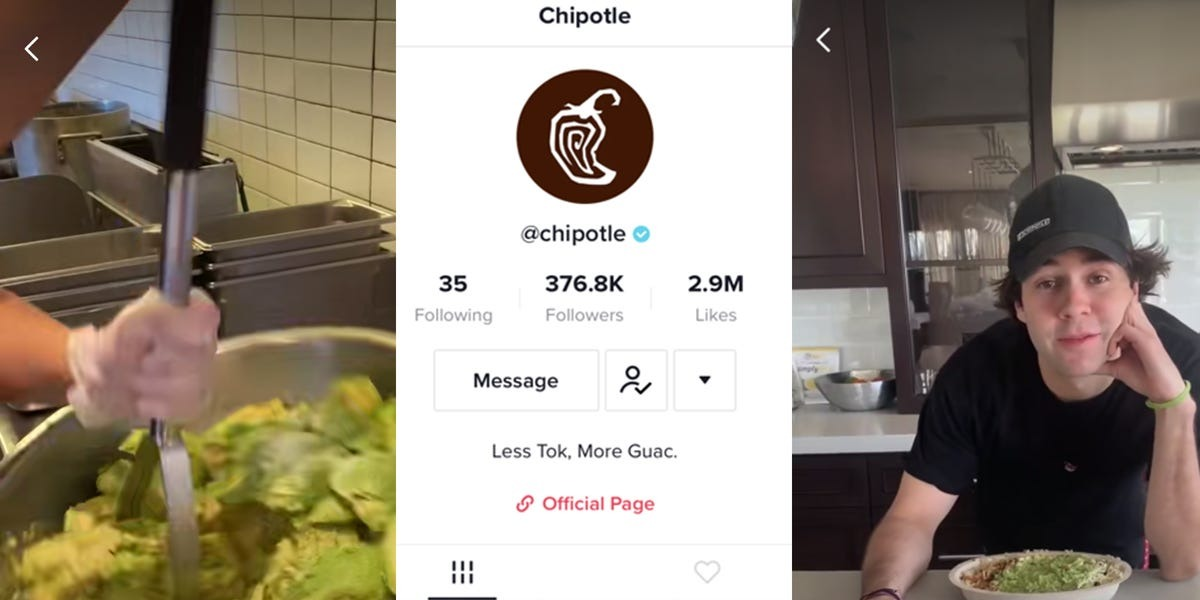
\includegraphics[width=1\textwidth,height=\textheight]{images/chipotle.jpg}
\caption{Chipotle: \#LidFlipChallenge}
\end{figure}

\hypertarget{youtube}{%
\subsubsection*{YouTube}\label{youtube}}
\addcontentsline{toc}{subsubsection}{YouTube}

YouTube's focus on video content allows for in-depth storytelling and the development of comprehensive narrative campaigns. The ``Like a Girl'' campaign by Always used YouTube's video platform to challenge gender stereotypes through emotional storytelling. The campaign's impactful narrative was well-suited to YouTube's format, enabling it to reach a wide audience and generate significant discussion.

\begin{figure}
\centering
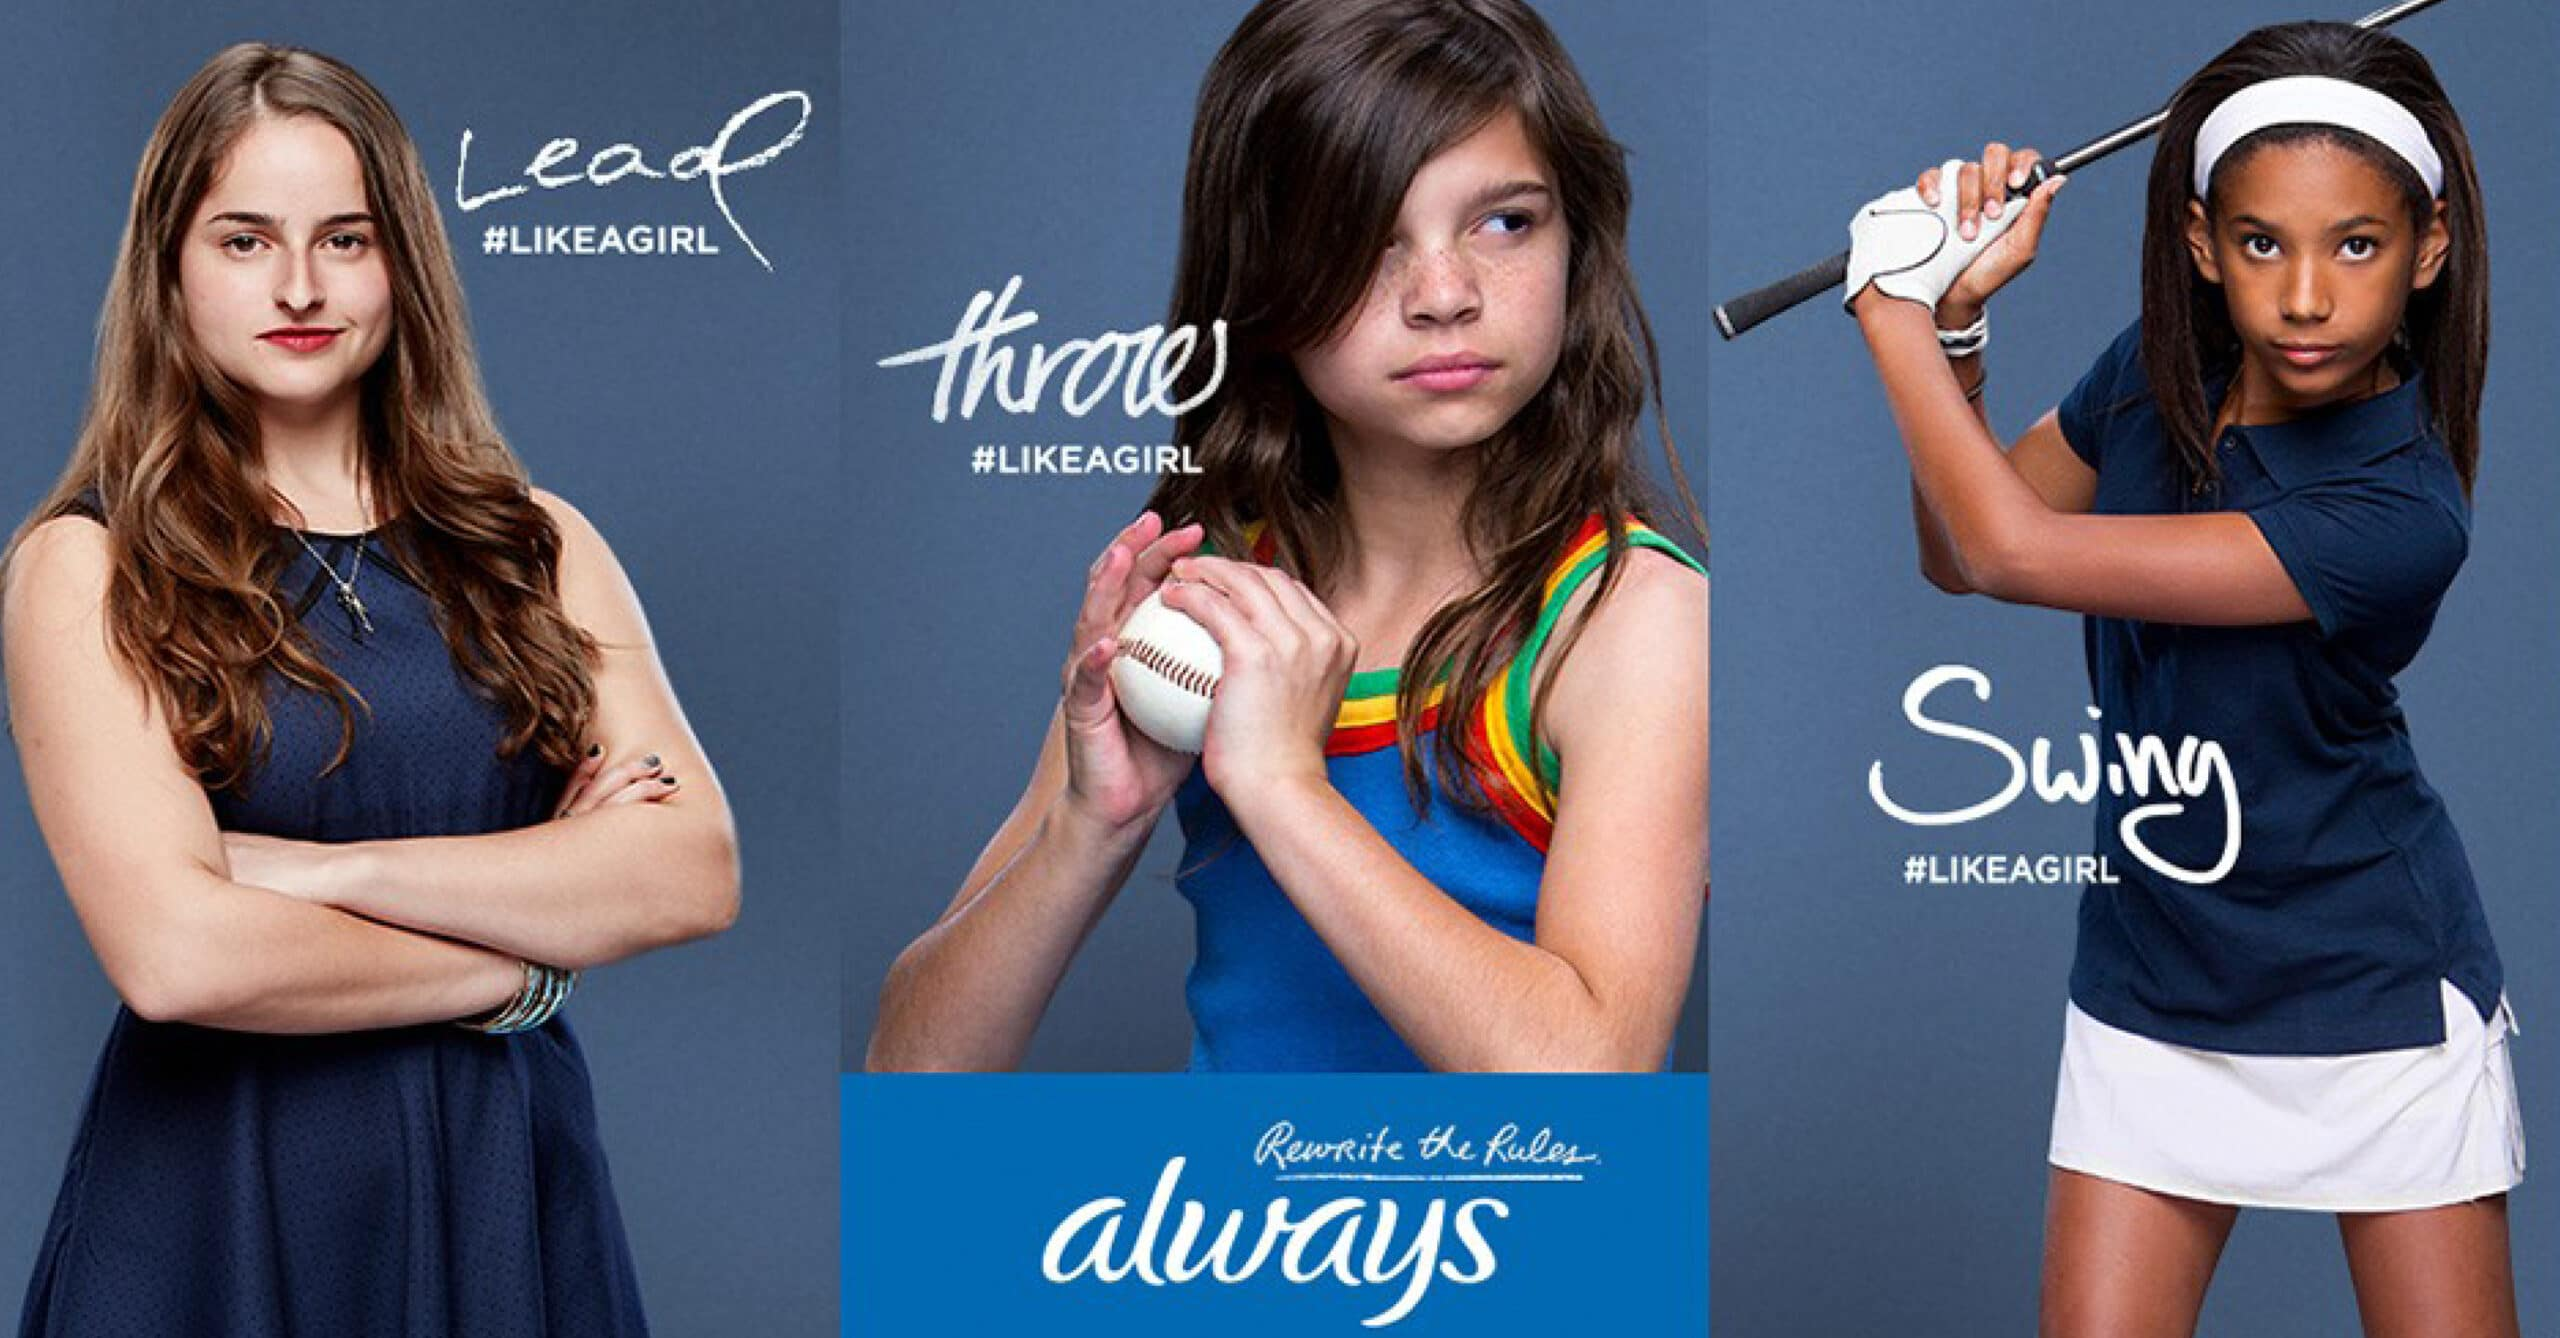
\includegraphics[width=1\textwidth,height=\textheight]{images/always.jpg}
\caption{Always: Like a Girl}
\end{figure}

In summary, understanding the unique attributes of each social media platform is crucial for crafting successful campaigns. By analyzing how different platforms have been leveraged in these examples, insights can be gained into the strategies that work best for each social media environment.

\hypertarget{campaign-goals-and-strategies}{%
\subsection*{Campaign Goals and Strategies}\label{campaign-goals-and-strategies}}
\addcontentsline{toc}{subsection}{Campaign Goals and Strategies}

\hypertarget{brand-awareness}{%
\subsubsection*{Brand Awareness}\label{brand-awareness}}
\addcontentsline{toc}{subsubsection}{Brand Awareness}

The goal of increasing brand awareness is often at the forefront of many social media campaigns. Strategies employed for this purpose need to capture the attention of a broad audience and create a memorable impression of the brand.

\textbf{\emph{Strategies}}:

\begin{itemize}
\tightlist
\item
  \textbf{Viral Content Creation}: Crafting content that has the potential to go viral, thus reaching a wider audience quickly.
\item
  \textbf{Influencer Partnerships}: Collaborating with influencers to tap into their followers and gain credibility.
\item
  \textbf{Leveraging Trending Topics}: Utilizing current trends or popular events to create relevant and engaging content that resonates with a larger audience.
\end{itemize}

\hypertarget{product-launch}{%
\subsubsection*{Product Launch}\label{product-launch}}
\addcontentsline{toc}{subsubsection}{Product Launch}

Launching a new product via social media requires a strategic approach that not only introduces the product but also generates excitement and anticipation.

\textbf{\emph{Strategies}}:

\begin{itemize}
\tightlist
\item
  \textbf{Teaser Campaigns}: Releasing snippets or previews of the product to build curiosity and anticipation.
\item
  \textbf{Influencer Reviews and Endorsements}: Having influencers review or endorse the product to provide authenticity and reach.
\item
  \textbf{Live Events and Launches}: Hosting live events or product reveals on social media platforms to engage the audience in real-time.
\end{itemize}

\hypertarget{community-building}{%
\subsubsection*{Community Building}\label{community-building}}
\addcontentsline{toc}{subsubsection}{Community Building}

Building a community around a brand or cause on social media is essential for fostering long-term engagement and loyalty.

\textbf{\emph{Strategies}}:

\begin{itemize}
\tightlist
\item
  \textbf{User Engagement}: Actively engaging with users through comments, messages, and posts to create a sense of community.
\item
  \textbf{Fostering Discussions}: Encouraging discussions around relevant topics to keep the audience engaged and connected.
\item
  \textbf{User-Generated Content Campaigns}: Inviting users to create and share their content related to the brand or cause, thus deepening their engagement and sense of belonging.
\end{itemize}

\hypertarget{social-change}{%
\subsubsection*{Social Change}\label{social-change}}
\addcontentsline{toc}{subsubsection}{Social Change}

Campaigns aimed at driving social change use social media as a platform to raise awareness and encourage action on various issues.

\textbf{\emph{Strategies}}:

\begin{itemize}
\tightlist
\item
  \textbf{Emotional Storytelling}: Using powerful narratives to connect with the audience on an emotional level and bring attention to the cause.
\item
  \textbf{Call-to-Action}: Including clear calls-to-action in campaign messages to encourage the audience to take specific steps towards supporting the cause.
\item
  \textbf{Partnerships with NGOs and Activists}: Collaborating with non-profit organizations and activists to lend credibility and reach a wider audience.
\end{itemize}

Each of these campaign goals requires a tailored set of strategies to effectively reach and engage the target audience. By dissecting these goals and examining the corresponding strategies, this section aims to provide a comprehensive understanding of how different objectives shape the approach and execution of successful social media campaigns.

\hypertarget{metrics-of-success}{%
\subsection*{Metrics of Success}\label{metrics-of-success}}
\addcontentsline{toc}{subsection}{Metrics of Success}

In the chapter ``Studying Successful Social Media Campaigns,'' an essential component of understanding and evaluating these campaigns is the identification and analysis of key performance indicators (KPIs). These metrics provide quantifiable evidence of a campaign's success and effectiveness. By examining these metrics, we can gain insights into how well a campaign achieved its objectives and engaged with its target audience. This section discusses the various metrics that are typically used to measure the success of social media campaigns.

\hypertarget{engagement-rates}{%
\subsubsection*{Engagement Rates}\label{engagement-rates}}
\addcontentsline{toc}{subsubsection}{Engagement Rates}

Engagement rates are critical indicators of how actively users interact with a campaign. High engagement rates generally suggest that the content is resonating with the audience, capturing their attention, and encouraging participation.

\textbf{\emph{Components}}:

\begin{itemize}
\tightlist
\item
  \textbf{Likes}: Reflects the number of users who positively react to the content.
\item
  \textbf{Shares}: Indicates how many times the content has been shared by users, amplifying its reach.
\item
  \textbf{Comments}: Provides insight into the level of conversation and discussion generated by the content.
\item
  \textbf{Other Interactions}: May include video views, clicks on links, or use of campaign-specific hashtags.
\end{itemize}

\hypertarget{conversion-rates}{%
\subsubsection*{Conversion Rates}\label{conversion-rates}}
\addcontentsline{toc}{subsubsection}{Conversion Rates}

Conversion rates measure the effectiveness of a campaign in driving users to take a specific desired action. This metric is crucial for campaigns aimed at achieving tangible outcomes like sales, sign-ups, or downloads.

\textbf{Calculation}: Conversion rate is calculated by dividing the number of conversions (desired actions taken) by the total number of visitors or interactions, and then multiplying by 100 to get a percentage.

\hypertarget{reach-and-impressions}{%
\subsubsection*{Reach and Impressions}\label{reach-and-impressions}}
\addcontentsline{toc}{subsubsection}{Reach and Impressions}

Reach and impressions provide insight into the extent and frequency of a campaign's visibility.

\textbf{Reach}: Refers to the total number of unique users who have seen the campaign content.

\textbf{Impressions}: Indicates the number of times the campaign content has been displayed, regardless of whether it was clicked or not.

\hypertarget{sentiment-analysis}{%
\subsubsection*{Sentiment Analysis}\label{sentiment-analysis}}
\addcontentsline{toc}{subsubsection}{Sentiment Analysis}

Sentiment analysis assesses the public's perception and emotional response to a campaign. This metric goes beyond mere numbers to understand the qualitative impact of the campaign.

\textbf{Approach}: Utilizing natural language processing (NLP) tools to analyze comments, posts, and mentions, determining whether the sentiment is positive, negative, or neutral.

\textbf{Importance}: Sentiment analysis helps gauge the public's feelings towards a campaign, providing insights into brand perception and campaign effectiveness.

In summary, these metrics form the backbone of campaign analysis in social media analytics. They provide measurable and actionable insights that help in understanding the effectiveness of a campaign and guiding future social media strategies. Analyzing these metrics requires a combination of quantitative analysis, for numerical data, and qualitative analysis, for understanding user sentiment and perception.

\hypertarget{visual-and-content-analysis}{%
\subsection*{Visual and Content Analysis}\label{visual-and-content-analysis}}
\addcontentsline{toc}{subsection}{Visual and Content Analysis}

In the chapter ``Studying Successful Social Media Campaigns,'' an in-depth analysis of the visual and content aspects of these campaigns is imperative. The visual elements and content style play a significant role in how a campaign is perceived and engaged with by its audience. This section focuses on the critical aspects of visual and content analysis, essential for understanding the success factors of social media campaigns.

\hypertarget{visual-elements}{%
\subsubsection*{Visual Elements}\label{visual-elements}}
\addcontentsline{toc}{subsubsection}{Visual Elements}

The visual appeal of a campaign is often the first point of interaction with the audience. It encompasses various elements that collectively contribute to the campaign's effectiveness.

\textbf{\emph{Components}}:

\begin{itemize}
\tightlist
\item
  \textbf{Use of Color}: Analyzing the color scheme used in the campaign and how it aligns with the brand's identity and the emotions it aims to evoke.
\item
  \textbf{Imagery}: The type of images used (photographs, illustrations, infographics) and their relevance to the campaign message.
\item
  \textbf{Video Style}: For video content, aspects such as cinematography, pacing, and visual effects are considered. This also includes how well the video content captures and retains viewer attention.
\item
  \textbf{Alignment with Brand Identity}: Assessing how the visual elements reinforce or complement the brand's overall identity and messaging.
\end{itemize}

\hypertarget{content-style}{%
\subsubsection*{Content Style}\label{content-style}}
\addcontentsline{toc}{subsubsection}{Content Style}

The style of content, encompassing tone, language, and format, plays a crucial role in how the message is conveyed and received by the audience.

\textbf{\emph{Considerations}}:

\begin{itemize}
\tightlist
\item
  \textbf{Tone}: Whether the campaign uses a formal, informal, humorous, or serious tone and how this aligns with the brand's voice and campaign objectives.
\item
  \textbf{Language}: The choice of words, phrases, and the overall linguistic style. This also includes considerations of language simplicity or complexity based on the target audience.
\item
  \textbf{Format}: The structure of the content, whether it's short-form posts, long-form articles, stories, tweets, etc., and how this format is suited to the message and platform.
\end{itemize}

\hypertarget{adaptation-to-platform}{%
\subsubsection*{Adaptation to Platform}\label{adaptation-to-platform}}
\addcontentsline{toc}{subsubsection}{Adaptation to Platform}

Each social media platform has unique characteristics and user expectations. The adaptation of visual and content style to these platforms is crucial for campaign effectiveness.

\textbf{\emph{Strategies}}:

\begin{itemize}
\tightlist
\item
  \textbf{Platform-Specific Customization}: Tailoring content to leverage platform-specific features, like Instagram's visual focus or Twitter's concise messaging.
\item
  \textbf{Consistency Across Platforms}: While customization is key, maintaining a consistent brand voice and visual style across platforms is essential for brand recognition.
\item
  \textbf{Responsive Adaptation}: Being responsive to the platform's changing trends and user behaviors and adapting the campaign strategy accordingly.
\end{itemize}

By thoroughly examining these visual and content aspects, one can gain a deeper understanding of the mechanisms and strategies that drive successful social media campaigns. This analysis serves as both an academic resource for understanding social media dynamics and a practical guide for professionals and marketers seeking to enhance their social media presence.

\hypertarget{lessons-learned-and-best-practices}{%
\section*{Lessons Learned and Best Practices}\label{lessons-learned-and-best-practices}}
\addcontentsline{toc}{section}{Lessons Learned and Best Practices}

\hypertarget{synthesizing-key-takeaways}{%
\subsection{Synthesizing Key Takeaways}\label{synthesizing-key-takeaways}}

The main lessons from the case studies can be summarized as follows:

\textbf{Targeted Content}: Successful campaigns often feature content that is meticulously tailored to the interests, needs, and preferences of their target audience.

\textbf{Authenticity}: Campaigns that resonate the most tend to exhibit a high degree of authenticity, aligning with the brand's core values and message.

\textbf{Engagement Strategies}: Effective campaigns actively engage their audience through interactive content, user-generated content initiatives, and responsive communication.

\textbf{Strategic Use of Platform Features}: Utilizing platform-specific features such as Instagram Stories, Twitter Polls, or TikTok challenges can significantly enhance campaign effectiveness.

\textbf{Data-Driven Approaches}: Leveraging analytics for insights into audience behavior and campaign performance is a common trait of successful campaigns.

\hypertarget{best-practices-in-campaign-execution}{%
\subsection{Best Practices in Campaign Execution}\label{best-practices-in-campaign-execution}}

Based on these takeaways, several best practices can be compiled:

\textbf{Content Creation}: Focus on creating high-quality, relevant, and engaging content. Visuals should be eye-catching and consistent with brand identity.

\textbf{Timing and Frequency}: Post content at times when the target audience is most active. Maintain a consistent posting schedule without overwhelming followers.

\textbf{Audience Engagement}: Encourage interaction by posing questions, creating polls, and responding to comments and messages.

\textbf{Platform-Specific Strategies}: Tailor content and tactics to the unique features and audience demographics of each platform. For instance, short-form videos for TikTok and professional articles for LinkedIn.

\textbf{Cross-Platform Integration}: Create a cohesive campaign experience across different platforms, adapting the content while maintaining a unified message.

\hypertarget{adaptability-and-innovation}{%
\subsection{Adaptability and Innovation}\label{adaptability-and-innovation}}

Adaptability and innovation are crucial in the ever-evolving landscape of social media:

\textbf{Keeping Pace with Trends}: Stay informed about the latest social media trends and algorithm changes to adjust strategies accordingly.

\textbf{Innovative Approaches}: Stand out by experimenting with new formats, technologies (like AR/VR), and creative storytelling.

\textbf{Continuous Learning}: Analyze ongoing campaign data to learn what works and adapt strategies in real-time.

\hypertarget{risk-management-and-ethics}{%
\subsection{Risk Management and Ethics}\label{risk-management-and-ethics}}

Finally, addressing the risks and ethical considerations:

\textbf{Anticipating Backlash}: Be prepared for potential negative responses by having a crisis management plan in place.

\textbf{Cultural Sensitivity}: Ensure that content is culturally sensitive and does not inadvertently offend any group.

\begin{figure}
\centering
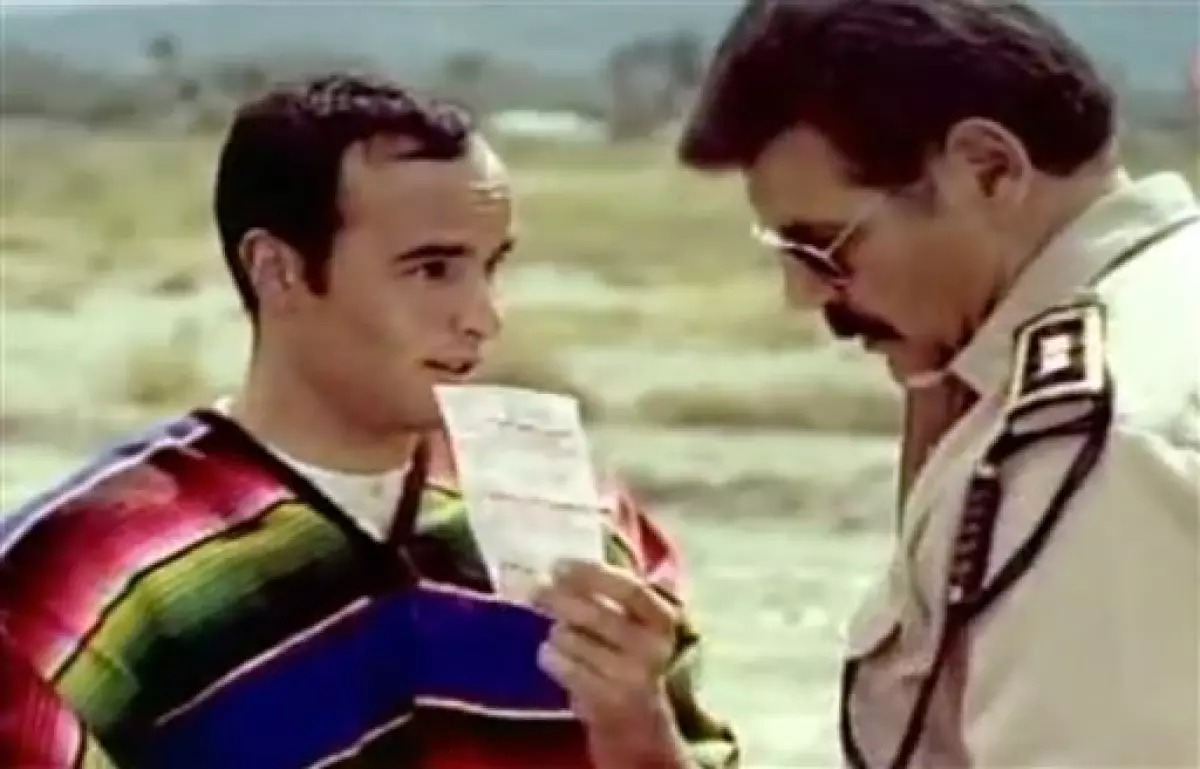
\includegraphics[width=1\textwidth,height=\textheight]{images/lottery-mexico.jpg}
\caption{Landon Donovan: Mexican Lottery Ad}
\end{figure}

\textbf{Transparency and Honesty}: Maintain transparency, especially when dealing with endorsements or sponsored content, to build trust with the audience.

\textbf{Data Privacy and Ethics}: Respect user privacy and adhere to data protection regulations.

In conclusion, synthesizing these key takeaways and best practices provides a comprehensive framework for designing and executing successful social media campaigns. By embracing adaptability, innovation, and a strong ethical foundation, campaigns can not only achieve their objectives but also contribute positively to the digital ecosystem.

\hypertarget{discussion-what-makes-a-campaign-successful}{%
\section*{Discussion: What Makes a Campaign Successful?}\label{discussion-what-makes-a-campaign-successful}}
\addcontentsline{toc}{section}{Discussion: What Makes a Campaign Successful?}

\hypertarget{defining-success-in-social-media-campaigns}{%
\subsection{Defining Success in Social Media Campaigns}\label{defining-success-in-social-media-campaigns}}

Success in social media campaigns can be subjective and varied, depending on several factors:

\textbf{Objective-Based Success}: The achievement of specific goals set prior to the campaign, which could range from increasing brand awareness to driving sales or promoting social causes.

\textbf{Scale and Reach}: For some campaigns, success is measured by the scale of reach and engagement, quantified by metrics such as likes, shares, and comments.

\textbf{Resource Efficiency}: Success for smaller brands might be defined by achieving maximum impact with limited resources.

\textbf{Long-Term Impact}: Beyond immediate metrics, the long-term effect on brand perception and customer loyalty is also a crucial measure of success.

\hypertarget{elements-of-a-successful-campaign}{%
\subsection{Elements of a Successful Campaign}\label{elements-of-a-successful-campaign}}

Analysis of successful campaigns reveals several common elements:

\textbf{Strong Narrative}: Campaigns like Dove's ``Real Beauty'' leveraged emotive storytelling to connect with audiences on a deeper level.

\textbf{Audience Understanding}: Successful campaigns demonstrate a deep understanding of the target audience's preferences, behaviors, and values.

\textbf{Authenticity}: Authentic campaigns, like Patagonia's environmental advocacy, resonate more with audiences seeking genuine brand interactions.

\textbf{Clear Call-to-Action}: Campaigns need to guide audiences on the desired action, whether it's purchasing a product, signing a petition, or joining a movement.

\textbf{Effective Use of Visuals and Hashtags}: Visually appealing content and memorable hashtags can significantly enhance a campaign's visibility and engagement.

\textbf{Engagement Strategies}: Tactics such as interactive polls, contests, and user-generated content initiatives encourage active participation.

\hypertarget{the-role-of-audience-interaction}{%
\subsection{The Role of Audience Interaction}\label{the-role-of-audience-interaction}}

Audience interaction plays a pivotal role in amplifying a campaign's reach and impact:

\textbf{User-Generated Content}: Campaigns like Starbucks' ``\#WhiteCupContest'' encouraged users to create content, boosting engagement and reach.

\textbf{Interactive Features}: Utilizing features like Instagram Stories polls or Twitter Q\&A sessions to foster a two-way conversation.

\textbf{Community Building}: Creating a sense of community around a brand or cause can lead to more meaningful and sustained engagement.

\hypertarget{challenges-and-overcoming-obstacles}{%
\subsection{Challenges and Overcoming Obstacles}\label{challenges-and-overcoming-obstacles}}

Successful campaigns often navigate various challenges:

\textbf{Changing Platform Algorithms}: Adapting to algorithm changes requires a flexible content strategy and a willingness to experiment with new formats.

\textbf{Audience Fatigue}: To combat audience fatigue, it's important to keep content fresh, relevant, and varied.

\textbf{Competition for Attention}: Standing out in a crowded digital space might involve leveraging emerging trends, niche marketing, or influencer collaborations.

\textbf{Case Study - Overcoming Obstacles}: An example is the Old Spice ``The Man Your Man Could Smell Like'' campaign, which rejuvenated a classic brand by using humor and an unconventional approach to challenge traditional advertising norms.

\begin{figure}
\centering
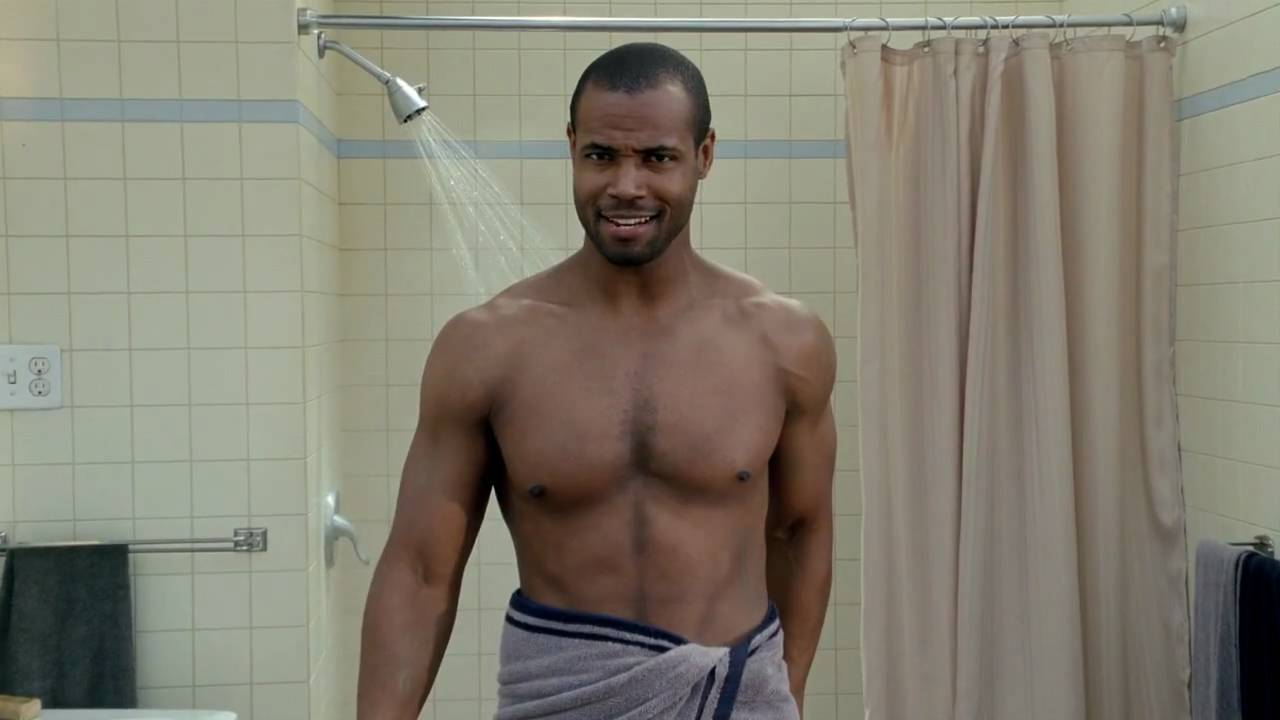
\includegraphics[width=1\textwidth,height=\textheight]{images/oldspice.jpg}
\caption{Old Spice: The Man Your Man Could Smell Like}
\end{figure}

In summary, a successful social media campaign is multifaceted, encompassing a clear understanding of objectives, audience, and the dynamic nature of social media platforms. By analyzing these elements and addressing the inherent challenges, future campaigns can be better equipped to navigate the complex landscape of social media marketing.

\hypertarget{data-collection-tools}{%
\chapter{Data Collection Tools}\label{data-collection-tools}}

\hypertarget{overview-of-analytics-tools}{%
\section*{Overview of Analytics Tools}\label{overview-of-analytics-tools}}
\addcontentsline{toc}{section}{Overview of Analytics Tools}

\hypertarget{introduction-to-analytics-tools}{%
\subsection*{Introduction to Analytics Tools}\label{introduction-to-analytics-tools}}
\addcontentsline{toc}{subsection}{Introduction to Analytics Tools}

In the realm of social media strategy, the deployment of analytics tools is not merely advantageous; it is essential. These tools furnish marketers, data analysts, and researchers with the capability to decipher vast amounts of data generated by social media platforms, transforming raw metrics into actionable insights. This transformation is crucial for understanding and enhancing user engagement, tailoring content to audience preferences, and measuring the efficacy of social media campaigns.

\hypertarget{importance-of-analytics-in-social-media-strategy}{%
\subsubsection*{Importance of Analytics in Social Media Strategy}\label{importance-of-analytics-in-social-media-strategy}}
\addcontentsline{toc}{subsubsection}{Importance of Analytics in Social Media Strategy}

Analytics tools serve as the cornerstone for informed decision-making in social media marketing. They allow for the tracking of key performance indicators (KPIs) such as likes, shares, comments, page views, and conversion rates. By analyzing these metrics, organizations can optimize their social media strategies to achieve specific objectives, whether they be increasing brand awareness, enhancing customer engagement, or driving sales. Moreover, analytics tools enable the identification of trends and patterns in user behavior, facilitating the prediction of future interactions and the tailoring of content to meet the evolving preferences of the target audience.

\hypertarget{role-in-understanding-user-engagement-and-behavior}{%
\subsubsection*{Role in Understanding User Engagement and Behavior}\label{role-in-understanding-user-engagement-and-behavior}}
\addcontentsline{toc}{subsubsection}{Role in Understanding User Engagement and Behavior}

Understanding user engagement and behavior is paramount in crafting a social media strategy that resonates with an audience. Analytics tools provide a window into the user's world, offering insights into what content performs well, the times users are most active, and the types of interactions that occur with the brand's social media presence. This understanding allows for the refinement of content strategies, ensuring that posts are both relevant and engaging to the audience. Furthermore, analytics can shed light on the customer journey, from initial contact through to conversion, highlighting opportunities to enhance the user experience and foster brand loyalty.

\hypertarget{overview-of-tool-capabilities-and-applications}{%
\subsubsection*{Overview of Tool Capabilities and Applications}\label{overview-of-tool-capabilities-and-applications}}
\addcontentsline{toc}{subsubsection}{Overview of Tool Capabilities and Applications}

The capabilities of analytics tools extend beyond mere data collection; they encompass a broad spectrum of functionalities designed to dissect and interpret social media data. These tools can track real-time interactions, segment audiences based on demographics or behavior, and measure the return on investment (ROI) of social media campaigns. Applications of these tools are varied and can range from simple tasks such as scheduling posts and monitoring hashtag performance to more complex analyses like sentiment analysis and predictive modeling.

For instance, R and RStudio, while not exclusively social media analytics tools, are powerful allies in the analysis and visualization of social media data. R, a programming language and software environment for statistical computing, coupled with RStudio, an integrated development environment (IDE) for R, enables researchers and analysts to perform sophisticated data analysis and create compelling visualizations. This combination is particularly useful for custom analyses that go beyond the capabilities of standard social media analytics tools, allowing for the exploration of user sentiment, trend analysis, and network analysis. Through packages designed specifically for social media data (like \texttt{twitteR} for Twitter data, \texttt{Rfacebook} for Facebook data, and others), users can collect, process, and analyze data in ways that are tailored to their specific research questions or business needs.

The strategic application of analytics tools, including the adept use of R and RStudio for custom data analysis, is indispensable in navigating the complex landscape of social media. These tools not only illuminate the path to enhanced engagement and strategic alignment but also empower organizations to leverage data-driven insights for competitive advantage.

\hypertarget{google-analytics}{%
\subsection*{Google Analytics}\label{google-analytics}}
\addcontentsline{toc}{subsection}{Google Analytics}

Google Analytics stands as a paramount tool in the domain of web analytics, offering extensive capabilities for tracking website traffic, analyzing user behavior, and integrating data from social media platforms. Its comprehensive suite of features enables organizations to glean actionable insights from their online presence, informing strategies that enhance user engagement and drive conversions. For social media analysts and marketers, Google Analytics provides a powerful means to measure the impact of social media on website traffic and to understand how users interact with their content across different channels.

\hypertarget{tracking-website-traffic-and-social-media-integration}{%
\subsubsection*{Tracking Website Traffic and Social Media Integration}\label{tracking-website-traffic-and-social-media-integration}}
\addcontentsline{toc}{subsubsection}{Tracking Website Traffic and Social Media Integration}

Google Analytics excels in its ability to track users' interactions with a website, offering detailed insights into the source of traffic, including direct visits, search engine referrals, and social media platforms. By integrating social media data, analysts can discern the effectiveness of social media campaigns in driving traffic to their website. This integration is crucial for understanding the role of social media within the broader digital marketing strategy, allowing organizations to attribute conversions and engagements directly to their social media efforts.

\textbf{Social Media Reporting}: Leveraging Google Analytics' social media reports, users can identify which platforms are generating the most traffic, the quality of this traffic in terms of engagement and conversion rates, and how users from different platforms behave once they land on the website.

\hypertarget{setting-up-and-interpreting-goals}{%
\subsubsection*{Setting Up and Interpreting Goals}\label{setting-up-and-interpreting-goals}}
\addcontentsline{toc}{subsubsection}{Setting Up and Interpreting Goals}

Goals in Google Analytics are used to track how well a website fulfills target objectives, such as form submissions, product purchases, or time spent on a page. Setting up goals allows marketers to measure conversions that originate from social media channels, providing a clear picture of social media ROI.

\textbf{Conversion Tracking}: By defining specific actions as goals, analysts can pinpoint which social media platforms contribute most to desired outcomes, enabling targeted strategy refinement.

\textbf{Funnel Analysis}: Through goal funnels, Google Analytics can show the path users take towards conversion, highlighting potential drop-off points and opportunities for optimization.

\hypertarget{audience-demographics-and-behavior-analysis}{%
\subsubsection*{Audience Demographics and Behavior Analysis}\label{audience-demographics-and-behavior-analysis}}
\addcontentsline{toc}{subsubsection}{Audience Demographics and Behavior Analysis}

Understanding who visits a website and how they interact with it is crucial for tailoring content and marketing strategies. Google Analytics offers in-depth analysis of audience demographics (age, gender, interests) and behavior (new vs.~returning users, frequency of visits, engagement metrics).

\textbf{Segmentation}: This feature allows for the segmentation of traffic from social media to analyze specific groups' behavior, providing insights into how different demographic segments interact with the website.

\textbf{Behavior Flow}: Visualizing the path users take through the site, from entry to exit, helps identify content that resonates with the audience, as well as potential obstacles in the user journey.

\hypertarget{utilizing-reports-for-social-media-strategy-refinement}{%
\subsubsection*{Utilizing Reports for Social Media Strategy Refinement}\label{utilizing-reports-for-social-media-strategy-refinement}}
\addcontentsline{toc}{subsubsection}{Utilizing Reports for Social Media Strategy Refinement}

The reports generated by Google Analytics are instrumental in refining social media strategies. By analyzing data on user interactions, conversions, and the effectiveness of different social media channels, organizations can make informed decisions about where to allocate resources and how to adjust their content and messaging for optimal engagement.

\textbf{Custom Reports}: Tailored reports can be created to focus on specific aspects of social media performance, offering customized insights that align with organizational goals.

\textbf{Integration with R \& RStudio}: For deeper analysis, data from Google Analytics can be exported and analyzed using R \& RStudio. This allows for the application of statistical models, trend analysis, and the creation of bespoke visualizations, providing a more nuanced understanding of the data.

Google Analytics offers a robust framework for tracking, analyzing, and optimizing the intersection of website traffic and social media engagement. When used in conjunction with advanced analytical tools like R \& RStudio, it enables a granular analysis of social media's impact on digital marketing objectives, empowering organizations to craft data-driven strategies that resonate with their audience and amplify their online presence.

\hypertarget{hootsuite}{%
\subsection*{Hootsuite}\label{hootsuite}}
\addcontentsline{toc}{subsection}{Hootsuite}

Hootsuite is a comprehensive social media management platform that empowers organizations and individuals to streamline their social media activities. From scheduling posts to monitoring conversations and analyzing performance metrics, Hootsuite provides a centralized dashboard for managing multiple social media accounts across various platforms. Its robust suite of tools is designed to enhance audience engagement, monitor brand reputation, and optimize social media strategies through data-driven insights.

\hypertarget{features-for-post-scheduling-and-social-media-monitoring}{%
\subsubsection*{Features for Post Scheduling and Social Media Monitoring}\label{features-for-post-scheduling-and-social-media-monitoring}}
\addcontentsline{toc}{subsubsection}{Features for Post Scheduling and Social Media Monitoring}

Hootsuite's post scheduling feature allows users to plan and publish content across different social media platforms from a single interface. This functionality not only saves time but also ensures that content reaches the audience at optimal times for engagement. In addition to scheduling, Hootsuite offers comprehensive monitoring capabilities, enabling users to track mentions, keywords, and trends in real-time. This is crucial for engaging with the audience promptly and managing brand reputation effectively.

\textbf{Streamlining Content Management}: Automating the posting process for consistency and efficiency.

\textbf{Real-time Engagement}: Monitoring social media feeds to respond quickly to user interactions, mentions, and direct messages.

\hypertarget{traffic-and-campaign-analysis-across-platforms}{%
\subsubsection*{Traffic and Campaign Analysis across Platforms}\label{traffic-and-campaign-analysis-across-platforms}}
\addcontentsline{toc}{subsubsection}{Traffic and Campaign Analysis across Platforms}

Hootsuite's analytics tools offer a detailed view of social media performance across platforms, enabling users to measure the impact of their campaigns and identify areas for improvement. By analyzing traffic, engagement rates, and conversion metrics, organizations can gauge the effectiveness of their social media strategies and make data-informed adjustments.

\textbf{Cross-Platform Analytics}: Aggregating data from various social media platforms to provide a unified view of social media performance.

\textbf{Campaign Tracking}: Monitoring specific campaigns to assess their reach, engagement, and overall success.

\hypertarget{utilizing-hootsuite-for-audience-engagement-and-brand-monitoring}{%
\subsubsection*{Utilizing Hootsuite for Audience Engagement and Brand Monitoring}\label{utilizing-hootsuite-for-audience-engagement-and-brand-monitoring}}
\addcontentsline{toc}{subsubsection}{Utilizing Hootsuite for Audience Engagement and Brand Monitoring}

Engaging with the audience and monitoring brand health are critical components of successful social media management. Hootsuite facilitates these processes by providing tools that help users listen to their audience and track sentiment regarding their brand. This proactive approach to engagement and monitoring helps in building a positive brand image and fostering a loyal community.

\textbf{Sentiment Analysis}: Gauging the mood and perceptions of the audience towards the brand or specific topics.

\textbf{Brand Health Monitoring}: Keeping tabs on brand mentions and sentiment to manage reputation and address potential issues promptly.

\hypertarget{reporting-and-analytics-capabilities}{%
\subsubsection*{Reporting and Analytics Capabilities}\label{reporting-and-analytics-capabilities}}
\addcontentsline{toc}{subsubsection}{Reporting and Analytics Capabilities}

Hootsuite's reporting and analytics capabilities are designed to transform social media data into actionable insights. Customizable reports allow users to focus on the metrics that matter most to their strategy, enabling the optimization of content and engagement tactics based on empirical evidence.

\textbf{Custom Reports}: Tailoring reports to highlight key performance indicators and trends relevant to organizational goals.

\textbf{Integration with R \& RStudio for Advanced Analysis}: For those requiring more in-depth analysis, Hootsuite's data can be exported and further analyzed using R \& RStudio. This allows for the application of statistical analysis, predictive modeling, and custom visualization to delve deeper into social media performance and user behavior.

Hootsuite stands out as a versatile tool for managing and optimizing social media activities. Its ability to schedule posts, monitor engagement, and analyze performance across platforms makes it an invaluable asset for social media marketers. When combined with the analytical power of R \& RStudio, Hootsuite's data can be leveraged for advanced analysis, offering deeper insights into social media strategy effectiveness and opportunities for refinement.

\hypertarget{buffer}{%
\subsection*{Buffer}\label{buffer}}
\addcontentsline{toc}{subsection}{Buffer}

Buffer is a highly regarded tool in the social media management space, known for its simplicity and effectiveness in scheduling posts, managing multiple accounts, and analyzing social media performance. It facilitates the planning and execution of social media strategies by offering a suite of features designed to optimize content distribution, engagement, and audience analysis. Buffer's analytics capabilities are instrumental for marketers and social media managers looking to refine their approach based on solid data insights.

\hypertarget{post-scheduling-and-management-for-multiple-accounts}{%
\subsubsection*{Post Scheduling and Management for Multiple Accounts}\label{post-scheduling-and-management-for-multiple-accounts}}
\addcontentsline{toc}{subsubsection}{Post Scheduling and Management for Multiple Accounts}

One of Buffer's core features is its ability to allow users to schedule posts across various social media platforms from a single dashboard. This streamlines the content management process, saving time and ensuring a consistent online presence. Moreover, Buffer supports the management of multiple accounts, making it easier for users to maintain a cohesive social media strategy across different channels and brands.

\textbf{Efficient Content Distribution}: Automating the scheduling of posts to ensure consistent content delivery at optimal times.

\textbf{Centralized Account Management}: Managing multiple social media accounts seamlessly from one platform.

\hypertarget{analyzing-engagement-trends-and-identifying-optimal-posting-times}{%
\subsubsection*{Analyzing Engagement Trends and Identifying Optimal Posting Times}\label{analyzing-engagement-trends-and-identifying-optimal-posting-times}}
\addcontentsline{toc}{subsubsection}{Analyzing Engagement Trends and Identifying Optimal Posting Times}

Buffer's analytics tools provide valuable insights into how content is performing on social media. By analyzing engagement trends, such as likes, shares, comments, and clicks, users can identify what content resonates most with their audience. Furthermore, Buffer offers data on optimal posting times, enabling users to schedule their content when it is most likely to be seen and engaged with by their target audience.

\textbf{Engagement Analysis}: Evaluating the performance of posts to understand what drives audience interaction.

\textbf{Optimal Timing Insights}: Leveraging data to determine the best times for posting to maximize visibility and engagement.

\hypertarget{understanding-audience-demographics-and-preferences}{%
\subsubsection*{Understanding Audience Demographics and Preferences}\label{understanding-audience-demographics-and-preferences}}
\addcontentsline{toc}{subsubsection}{Understanding Audience Demographics and Preferences}

Gaining a deep understanding of the audience is crucial for tailoring content and engagement strategies. Buffer helps in this regard by providing detailed insights into audience demographics and preferences. This information allows social media managers to create more targeted and relevant content that appeals to the specific interests and needs of their audience.

\textbf{Audience Segmentation}: Analyzing audience data to segment users based on demographics, interests, and behavior.

\textbf{Content Customization}: Using insights gained from audience analysis to inform content creation and curation.

\hypertarget{integrating-buffer-analytics-into-social-media-planning}{%
\subsubsection*{Integrating Buffer Analytics into Social Media Planning}\label{integrating-buffer-analytics-into-social-media-planning}}
\addcontentsline{toc}{subsubsection}{Integrating Buffer Analytics into Social Media Planning}

The insights gained from Buffer's analytics can be a goldmine for social media planning. By integrating these insights into the strategic planning process, organizations can make informed decisions about content creation, posting schedules, and engagement tactics. Buffer's analytics help in identifying successful content types and strategies, guiding the optimization of future social media efforts for better performance.

\textbf{Strategic Decision-Making}: Utilizing analytics to inform content strategy, campaign planning, and resource allocation.

\textbf{Advanced Analysis with R \& RStudio}: For deeper dives into social media data, Buffer's analytics can be exported and analyzed using R \& RStudio. This allows for sophisticated statistical analysis, trend detection, and the creation of custom visualizations to uncover deeper insights into social media performance and audience behavior.

Buffer stands out as an essential tool for managing and optimizing social media activities. Its strengths in post scheduling, engagement analysis, audience insights, and strategic integration make it a valuable asset for anyone looking to enhance their social media presence. When combined with the analytical capabilities of R \& RStudio, Buffer's data can provide even more nuanced insights, empowering users to craft data-driven, effective social media strategies.

\hypertarget{comparative-analysis-1}{%
\subsection*{Comparative Analysis}\label{comparative-analysis-1}}
\addcontentsline{toc}{subsection}{Comparative Analysis}

In the landscape of social media analytics tools, choosing the right platform can be a daunting task given the variety of options available, each with its unique set of features, strengths, and limitations. A comparative analysis of prominent tools like Google Analytics, Hootsuite, Buffer, and the integration of R \& RStudio provides valuable insights into how these tools can be leveraged to meet organizational goals. This section aims to dissect these aspects to aid in the decision-making process, ensuring that organizations select the most appropriate tools for their specific needs.

\hypertarget{comparing-features-strengths-and-limitations}{%
\subsubsection*{Comparing Features, Strengths, and Limitations}\label{comparing-features-strengths-and-limitations}}
\addcontentsline{toc}{subsubsection}{Comparing Features, Strengths, and Limitations}

\textbf{Google Analytics} excels in providing detailed insights into website traffic and user behavior, including the impact of social media referrals. Its strengths lie in its comprehensive tracking capabilities, robust reporting, and ability to analyze audience demographics and behavior. However, its focus is more on website analytics rather than direct social media engagement or content management.

\textbf{Hootsuite} offers a wide array of features for managing social media accounts, including post scheduling, real-time monitoring, and engagement tools. It stands out for its dashboard that consolidates multiple social media platforms, allowing for efficient management and analytics across channels. Its limitations may include a learning curve for new users and the potential need for additional integrations for deeper analytics.

\textbf{Buffer} focuses on simplifying social media scheduling and analytics, providing users with intuitive tools for content planning and performance analysis. It is particularly strong in user-friendly scheduling features and straightforward analytics. However, it may not offer the depth of analytics or the comprehensive platform coverage seen in more specialized tools.

\textbf{R \& RStudio}, while not a direct social media management tool, offer unparalleled customization and depth in data analysis. Their strengths lie in the ability to conduct sophisticated statistical analyses, create custom visualizations, and handle large datasets. The primary limitation is the requirement of programming knowledge, which may present a barrier to entry for those unfamiliar with R.

\hypertarget{decision-making-criteria-for-tool-selection}{%
\subsubsection*{Decision-making Criteria for Tool Selection}\label{decision-making-criteria-for-tool-selection}}
\addcontentsline{toc}{subsubsection}{Decision-making Criteria for Tool Selection}

Selecting the right tool(s) hinges on several criteria:

\textbf{Organizational Objectives}: Whether the focus is on enhancing engagement, driving website traffic, or analyzing user behavior will influence tool choice.

\textbf{Technical Expertise}: The in-house team's familiarity with analytics tools and programming languages like R can determine the feasibility of using more complex platforms.

\textbf{Integration Needs}: The ability of the tool to integrate with existing systems and platforms used by the organization.

\textbf{Feature Requirements}: Prioritizing features such as real-time monitoring, detailed reporting, or predictive analytics based on strategic needs.

\hypertarget{customization-and-scalability-of-tools}{%
\subsubsection*{Customization and Scalability of Tools}\label{customization-and-scalability-of-tools}}
\addcontentsline{toc}{subsubsection}{Customization and Scalability of Tools}

The ability to customize and scale the tool according to changing business needs is crucial. R \& RStudio offer the highest level of customization through programming, allowing for tailored analyses and visualizations. Tools like Hootsuite and Buffer provide scalability through various subscription plans, but customization in terms of analytics may be limited compared to the flexibility R provides.

\hypertarget{cost-benefit-analysis-for-different-organizational-needs}{%
\subsubsection*{Cost-benefit Analysis for Different Organizational Needs}\label{cost-benefit-analysis-for-different-organizational-needs}}
\addcontentsline{toc}{subsubsection}{Cost-benefit Analysis for Different Organizational Needs}

Evaluating the cost against the potential benefits of each tool is essential for making an informed decision. While Google Analytics provides a robust set of features for free, advanced features may require a subscription. Hootsuite and Buffer offer tiered pricing plans, catering to different sizes of businesses and their specific needs. R \& RStudio, being open-source, present a cost-effective option for data analysis, with the primary investment being in the development of expertise to use them effectively.

The selection of social media analytics tools requires a careful consideration of the organization's specific goals, technical capabilities, and budget constraints. By understanding the unique features, strengths, and limitations of each tool, as well as their customization potential and scalability, organizations can make an informed choice that aligns with their strategic objectives and resource availability. The integration of advanced data analysis tools like R \& RStudio can further enhance the depth and breadth of insights, offering a competitive edge in the ever-evolving social media landscape.

\hypertarget{methods-for-data-collection}{%
\section*{Methods for Data Collection}\label{methods-for-data-collection}}
\addcontentsline{toc}{section}{Methods for Data Collection}

\hypertarget{understanding-apis}{%
\subsection*{Understanding APIs}\label{understanding-apis}}
\addcontentsline{toc}{subsection}{Understanding APIs}

Application Programming Interfaces (APIs) are fundamental to the ecosystem of social media data collection, serving as conduits through which data can be systematically accessed and retrieved from social media platforms. APIs allow for the efficient collection of large volumes of data, facilitating the analysis of user interactions, engagement patterns, and trending content. This section delves into the role of APIs in social media analytics, provides an overview of APIs from major platforms, and discusses the inherent limitations and possibilities they present.

\hypertarget{role-of-apis-in-social-media-data-collection}{%
\subsubsection*{Role of APIs in Social Media Data Collection}\label{role-of-apis-in-social-media-data-collection}}
\addcontentsline{toc}{subsubsection}{Role of APIs in Social Media Data Collection}

APIs play a pivotal role in enabling researchers, marketers, and analysts to gather data from social media platforms. They provide structured access to social media data, allowing for the retrieval of information such as user posts, comments, likes, and follower counts. This access is crucial for performing sentiment analysis, trend tracking, and understanding audience demographics. APIs thus serve as the backbone for many social media analytics tools, enabling them to offer users insights into the performance of their content and strategies.

\textbf{Automated Data Retrieval}: APIs facilitate the automated collection of social media data, enabling efficient and systematic data gathering processes.

\textbf{Real-time Analysis}: Many APIs allow for the collection of real-time data, making it possible to monitor current trends and user reactions as they happen.

\hypertarget{overview-of-major-social-media-platforms-apis}{%
\subsubsection*{Overview of Major Social Media Platforms' APIs}\label{overview-of-major-social-media-platforms-apis}}
\addcontentsline{toc}{subsubsection}{Overview of Major Social Media Platforms' APIs}

Each major social media platform offers its own API, each with unique functionalities and data access levels.

\textbf{Twitter API}: Offers extensive access to tweet data, user profiles, and engagement metrics. It is widely used for trend analysis, sentiment analysis, and monitoring public opinion.

\textbf{Facebook Graph API}: Allows access to a broad range of data on Facebook, including user posts, comments, and page analytics. It is crucial for understanding audience engagement on Facebook pages and profiles.

\textbf{Instagram Graph API}: Provides insights into Instagram business and creator accounts, including post performance, audience data, and story analytics. It supports content planning and performance analysis on Instagram.

\textbf{LinkedIn API}: Offers access to data on professional networking activities, including user profiles, connections, and interactions. It is valuable for B2B marketing and professional brand analysis.

\hypertarget{limitations-and-possibilities-of-api-data-collection}{%
\subsubsection*{Limitations and Possibilities of API Data Collection}\label{limitations-and-possibilities-of-api-data-collection}}
\addcontentsline{toc}{subsubsection}{Limitations and Possibilities of API Data Collection}

While APIs offer significant advantages for social media data collection, they come with limitations that researchers and analysts must navigate.

\textbf{Rate Limiting and Data Caps}: Most social media platforms impose limits on the number of requests that can be made to their APIs within a certain timeframe, potentially restricting the volume of data that can be collected.

\textbf{Access Restrictions}: Access to certain types of data may be restricted based on privacy policies and user settings, limiting the completeness of data collection.

\textbf{Data Complexity}: The data retrieved through APIs can be complex and require significant processing and analysis to derive meaningful insights.

However, the possibilities offered by API data collection are vast. With the right tools and techniques, such as those provided by R \& RStudio, analysts can overcome some of these limitations by efficiently processing and analyzing large datasets, extracting trends, and deriving insights that inform strategic decision-making. The use of R, in particular, allows for the customization of data collection and analysis processes, enabling researchers to tailor their approaches to meet specific research questions and organizational needs.

Understanding the role, capabilities, and limitations of social media APIs is crucial for effective social media data collection. Despite the challenges, the strategic use of APIs in conjunction with powerful analytical tools like R \& RStudio can unlock a wealth of insights into social media behavior and trends, providing a solid foundation for data-driven decision-making in social media strategy.

\hypertarget{api-usage-in-practice}{%
\subsection*{API Usage in Practice}\label{api-usage-in-practice}}
\addcontentsline{toc}{subsection}{API Usage in Practice}

Practical engagement with Application Programming Interfaces (APIs) is a cornerstone activity in the domain of social media analytics. This involves a series of steps from obtaining the necessary access and permissions to efficiently managing data quotas and structuring the data for analysis. The dynamic nature of social media platforms and the vast volume of data generated require a nuanced approach to API usage. This section outlines the practical aspects of utilizing APIs for social media data collection, focusing on the challenges and strategies involved in accessing and managing data.

\hypertarget{obtaining-access-and-permissions}{%
\subsubsection*{Obtaining Access and Permissions}\label{obtaining-access-and-permissions}}
\addcontentsline{toc}{subsubsection}{Obtaining Access and Permissions}

Access to social media APIs is typically controlled through an application process, where developers or researchers must register their project and obtain API keys or access tokens. This process is designed to protect user data and ensure that access is granted for legitimate purposes.

\textbf{Registration}: Users must create an account on the social media platform's developer portal and register their application, detailing its purpose and scope.

\textbf{API Keys and Access Tokens}: Upon approval, the platform issues API keys or access tokens, which are used to authenticate requests to the API.

\textbf{Permissions and Scopes}: Access to different types of data may require specific permissions, which need to be explicitly requested. The scope of access granted can vary significantly depending on the platform's policies and the nature of the application.

\hypertarget{navigating-rate-limits-and-data-quotas}{%
\subsubsection*{Navigating Rate Limits and Data Quotas}\label{navigating-rate-limits-and-data-quotas}}
\addcontentsline{toc}{subsubsection}{Navigating Rate Limits and Data Quotas}

Social media platforms impose rate limits and data quotas to manage the load on their servers and protect user data. These restrictions can significantly impact the scope and speed of data collection efforts.

\textbf{Understanding Rate Limits}: Rate limits specify the number of API requests that can be made within a given timeframe. Exceeding these limits can result in temporary blocks or suspension of API access.

\textbf{Managing Data Quotas}: Data quotas limit the volume of data that can be retrieved through the API. It is essential to plan data collection activities to stay within these quotas.

\textbf{Strategies for Efficient Data Collection}: Implementing strategies such as caching responses, staggering requests, and using webhooks (if available) can help mitigate the impact of rate limits and data quotas.

\hypertarget{working-with-api-responses-and-data-structuring}{%
\subsubsection*{Working with API Responses and Data Structuring}\label{working-with-api-responses-and-data-structuring}}
\addcontentsline{toc}{subsubsection}{Working with API Responses and Data Structuring}

The data retrieved through social media APIs typically comes in a structured format, such as JSON or XML, which requires parsing and processing to extract meaningful information.

\textbf{Parsing API Responses}: Tools and libraries in R, such as \texttt{jsonlite} for JSON data, can be used to parse API responses and convert them into a more manageable format for analysis.

\textbf{Data Structuring}: Once parsed, the data needs to be structured into a format suitable for analysis. This may involve transforming the data into data frames, filtering irrelevant information, and aggregating data points for higher-level analysis.

\textbf{Dealing with Complexity}: Social media data can be complex, with nested structures and linked objects. Understanding the data model of the social media platform's API is crucial for effective data structuring and analysis.

Integrating R and RStudio into the workflow for API data collection enhances the capability to handle large datasets, apply complex transformations, and perform sophisticated analyses. R's comprehensive ecosystem of packages and RStudio's user-friendly interface support a range of activities from data collection to visualization and reporting. By mastering the practical aspects of API usage, including obtaining access, navigating rate limits, and structuring data, analysts and researchers can unlock the full potential of social media data to inform strategic decisions and uncover insights into digital behaviors and trends.

\hypertarget{web-scraping-techniques}{%
\subsection*{Web Scraping Techniques}\label{web-scraping-techniques}}
\addcontentsline{toc}{subsection}{Web Scraping Techniques}

Web scraping is a powerful technique for extracting data from websites and social media platforms, serving as a complement or alternative to API-based data collection. Unlike APIs, which provide data in a structured format based on predefined access rules, web scraping involves programmatically navigating and extracting data from the HTML of web pages. This section explores the fundamentals of web scraping, the tools and languages that facilitate effective data extraction, and the ethical and legal considerations that govern its use.

\hypertarget{introduction-to-web-scraping-vs.-api-use}{%
\subsubsection*{Introduction to Web Scraping vs.~API Use}\label{introduction-to-web-scraping-vs.-api-use}}
\addcontentsline{toc}{subsubsection}{Introduction to Web Scraping vs.~API Use}

Web scraping and API use are two primary methods for collecting data from the web and social media platforms. While APIs offer a direct route to data provided by the platform, subject to rate limits and access permissions, web scraping allows for more flexible data collection by extracting information directly from the webpage.

\textbf{Flexibility and Control}: Web scraping provides flexibility in data collection, allowing for the extraction of data that may not be available through APIs.

\textbf{Data Availability}: APIs provide structured, reliable data access within the platform's limitations. In contrast, web scraping can access any publicly visible information, though it requires parsing and structuring the data post-collection.

\hypertarget{tools-and-languages-for-effective-scraping}{%
\subsubsection*{Tools and Languages for Effective Scraping}\label{tools-and-languages-for-effective-scraping}}
\addcontentsline{toc}{subsubsection}{Tools and Languages for Effective Scraping}

Several tools and programming languages support web scraping, with Python and R being among the most popular due to their libraries and frameworks designed for this purpose.

\textbf{Python}: Libraries such as BeautifulSoup and Scrapy are widely used for web scraping, offering robust features for HTML parsing and data extraction.

\textbf{R}: The \texttt{rvest} package in R simplifies web scraping by providing functions to read and manipulate web page contents. Combined with RStudio, it offers a comprehensive environment for data collection, processing, and analysis.

\hypertarget{ethical-and-legal-considerations-in-web-scraping}{%
\subsubsection*{Ethical and Legal Considerations in Web Scraping}\label{ethical-and-legal-considerations-in-web-scraping}}
\addcontentsline{toc}{subsubsection}{Ethical and Legal Considerations in Web Scraping}

Web scraping operates in a complex ethical and legal landscape, necessitating careful consideration of the sources from which data is collected.

\textbf{Respecting \texttt{robots.txt}}: Websites use \texttt{robots.txt} files to define rules about what parts of the site can be accessed by automated agents. Ethical web scraping involves adhering to these rules.

\textbf{Legal Restrictions}: The legality of web scraping varies by jurisdiction and specific website terms of service. It is crucial to review and comply with these terms and applicable laws, such as the Computer Fraud and Abuse Act (CFAA) in the United States.

\textbf{Privacy Concerns}: Collecting data from public websites must be balanced with respect for individual privacy, especially when dealing with personal or sensitive information.

\hypertarget{overcoming-technical-challenges-in-scraping-activities}{%
\subsubsection*{Overcoming Technical Challenges in Scraping Activities}\label{overcoming-technical-challenges-in-scraping-activities}}
\addcontentsline{toc}{subsubsection}{Overcoming Technical Challenges in Scraping Activities}

Web scraping presents several technical challenges, from navigating complex website structures to handling dynamic content loaded via JavaScript.

\textbf{Dynamic Content}: Many modern websites use JavaScript to load content dynamically, which can be challenging to scrape using traditional methods. Tools like Selenium or R's \texttt{RSelenium} package can automate web browsers to interact with dynamic content.

\textbf{Data Structuring}: Extracted data often requires significant cleaning and structuring to be useful for analysis. R provides a suite of tools for data manipulation and cleaning, such as \texttt{dplyr} and \texttt{tidyr}, which are essential for preparing scraped data.

\textbf{Rate Limiting and IP Blocking}: Websites may limit the rate of requests or block IP addresses that make too many rapid requests. Implementing delays between requests and using proxy servers can help mitigate these issues.

Web scraping, when done responsibly and legally, is an invaluable technique for data collection, offering access to a wide range of data that may not be accessible through official APIs. The integration of web scraping methodologies with R \& RStudio enhances the capacity for in-depth analysis, providing researchers and analysts with the tools necessary to extract, process, and analyze web data effectively. However, it is imperative to navigate the ethical and legal considerations carefully to ensure that web scraping practices respect the rights of data owners and comply with legal standards.

\hypertarget{real-time-data-collection}{%
\subsection*{Real-time Data Collection}\label{real-time-data-collection}}
\addcontentsline{toc}{subsection}{Real-time Data Collection}

In the fast-paced environment of social media, real-time data collection is crucial for capturing the dynamics of user interactions, trending topics, and emerging narratives as they unfold. This capability enables organizations and researchers to react promptly to online conversations, adjust strategies in response to live events, and leverage trending moments for enhanced engagement. This section outlines the importance and applications of real-time data, explores tools and technologies for live data collection, and discusses strategies for analyzing and responding to trends as they develop.

\hypertarget{importance-and-applications-of-real-time-data}{%
\subsubsection*{Importance and Applications of Real-time Data}\label{importance-and-applications-of-real-time-data}}
\addcontentsline{toc}{subsubsection}{Importance and Applications of Real-time Data}

Real-time data collection from social media platforms offers immediate insights into public opinion, user behavior, and content performance, providing a competitive edge in both academic research and strategic marketing.

\textbf{Crisis Monitoring and Management}: Real-time data allows for the quick detection of potential crises or negative sentiment, enabling timely responses to mitigate potential damage.

\textbf{Event and Campaign Tracking}: Live data collection supports the monitoring of social media activities related to specific events or marketing campaigns, facilitating adjustments to optimize engagement and reach.

\textbf{Trend Discovery}: Identifying and engaging with trending topics in real-time can significantly increase visibility and audience engagement.

\hypertarget{tools-and-technologies-for-live-data-collection}{%
\subsubsection*{Tools and Technologies for Live Data Collection}\label{tools-and-technologies-for-live-data-collection}}
\addcontentsline{toc}{subsubsection}{Tools and Technologies for Live Data Collection}

Several tools and technologies are specifically designed to facilitate the real-time collection and analysis of social media data, with some offering integration capabilities with R \& RStudio for advanced analytics.

\textbf{Social Media APIs}: Many social media platforms offer streaming APIs that provide real-time access to public posts, tweets, and interactions. For instance, the Twitter Streaming API allows for the collection of tweets as they are posted.

\textbf{Third-party Tools}: Platforms like DataSift and Gnip provide access to real-time social media data streams, offering aggregated data across multiple social media platforms.

\textbf{R Packages}: Packages such as \texttt{streamR} for R provide interfaces to streaming APIs, enabling the collection and analysis of live data directly within the R environment.

\hypertarget{analyzing-and-responding-to-trends-in-real-time}{%
\subsubsection*{Analyzing and Responding to Trends in Real-time}\label{analyzing-and-responding-to-trends-in-real-time}}
\addcontentsline{toc}{subsubsection}{Analyzing and Responding to Trends in Real-time}

The ability to analyze and respond to real-time data requires a combination of automated data collection, rapid analysis techniques, and strategic planning to leverage insights effectively.

\textbf{Automated Monitoring and Alerts}: Setting up automated systems to monitor for specific keywords, hashtags, or sentiment can help in identifying trends as they emerge. Tools like \texttt{Shiny} in R can be used to create interactive, real-time dashboards for data visualization and monitoring.

\textbf{Rapid Analysis Techniques}: Utilizing R's capabilities for text analysis, sentiment analysis, and statistical modeling enables quick interpretation of real-time data. This can inform immediate strategic decisions, from content adjustment to crisis response.

\textbf{Engagement Strategies}: Based on real-time analytics, organizations can develop responsive engagement strategies, such as participating in trending conversations, adjusting ad spend, or publishing content aligned with current trends.

Real-time data collection and analysis offer invaluable insights into the ever-changing landscape of social media, providing the means to engage with audiences more effectively and make informed decisions based on live data. Integrating these practices with the analytical power of R \& RStudio enhances the ability to dissect large volumes of real-time data, uncover patterns, and respond to social media dynamics with precision and agility. By leveraging these tools and technologies, researchers and practitioners can stay at the forefront of social media trends, maximizing impact and engagement in an increasingly connected world.

\hypertarget{data-collection-challenges}{%
\subsection*{Data Collection Challenges}\label{data-collection-challenges}}
\addcontentsline{toc}{subsection}{Data Collection Challenges}

Collecting data from social media platforms, while rich in potential insights, presents a myriad of challenges ranging from managing vast and complex datasets to navigating the evolving landscape of platform policies and technical limitations. This section delves into the common hurdles encountered in social media data collection, specifically focusing on handling large and unstructured datasets, adapting to platform API changes and restrictions, and ensuring the quality and relevance of the data collected. It also offers strategies for overcoming these challenges, leveraging the capabilities of R \& RStudio to facilitate robust and efficient data collection processes.

\hypertarget{handling-large-and-unstructured-datasets}{%
\subsubsection*{Handling Large and Unstructured Datasets}\label{handling-large-and-unstructured-datasets}}
\addcontentsline{toc}{subsubsection}{Handling Large and Unstructured Datasets}

Social media platforms generate immense volumes of data daily, characterized by their unstructured nature, including text, images, videos, and user interactions. Managing and analyzing such datasets require sophisticated tools and techniques.

\textbf{Big Data Technologies}: Integrating R with big data technologies like Apache Hadoop or Spark can help process and analyze large datasets. Packages such as \texttt{sparklyr} offer a seamless interface between R and Spark, allowing for the distributed processing of large datasets.

\textbf{Data Structuring and Cleaning}: Utilizing R packages like \texttt{tidyr} for tidying data and \texttt{dplyr} for data manipulation can significantly streamline the process of structuring and cleaning unstructured datasets, making them more amenable to analysis.

\hypertarget{adapting-to-platform-api-changes-and-restrictions}{%
\subsubsection*{Adapting to Platform API Changes and Restrictions}\label{adapting-to-platform-api-changes-and-restrictions}}
\addcontentsline{toc}{subsubsection}{Adapting to Platform API Changes and Restrictions}

Social media platforms frequently update their APIs and impose new restrictions on data access, posing significant challenges to data collection efforts. These changes can affect the scope of data available and the methods used for collection.

\textbf{Staying Informed}: Regularly monitoring platform developer blogs and API documentation is crucial for staying up-to-date with changes.

\textbf{Flexible Data Collection Frameworks}: Developing flexible data collection scripts in R that can be easily modified to accommodate API changes. Utilizing abstraction layers or wrapper packages in R, such as \texttt{httr} for handling HTTP requests, can simplify the process of adapting to API changes.

\hypertarget{ensuring-data-quality-and-relevance}{%
\subsubsection*{Ensuring Data Quality and Relevance}\label{ensuring-data-quality-and-relevance}}
\addcontentsline{toc}{subsubsection}{Ensuring Data Quality and Relevance}

The quality and relevance of collected data are paramount for meaningful social media analysis. Challenges include filtering out irrelevant content, verifying the authenticity of data, and addressing biases.

\textbf{Data Filtering and Preprocessing}: Implementing robust data filtering mechanisms using R to remove irrelevant or redundant information. Packages such as \texttt{stringr} for string manipulation and \texttt{lubridate} for date/time operations are essential for preprocessing tasks.

\textbf{Addressing Biases}: Identifying and mitigating biases in data collection is critical for ensuring the representativeness of the dataset. Techniques such as stratified sampling can be applied using R to ensure diverse and representative data collection.

\textbf{Verification and Validation}: Employing techniques to verify the authenticity of the data and validate its relevance to the research questions or business objectives. This may include sentiment analysis using packages like \texttt{syuzhet} or \texttt{tm} for text mining to assess the sentiment and thematic relevance of the data.

Overcoming these challenges requires a combination of staying informed about the latest platform developments, employing flexible and robust data collection frameworks, and applying rigorous data processing and analysis techniques. The versatility of R \& RStudio, through its vast ecosystem of packages and its capability for integration with other technologies, provides a powerful platform for navigating the complexities of social media data collection. By leveraging these tools, researchers and practitioners can enhance the efficiency, accuracy, and relevance of their social media analytics efforts, unlocking deeper insights and driving more informed decisions.

\hypertarget{ethical-considerations-in-data-collection}{%
\section*{Ethical Considerations in Data Collection}\label{ethical-considerations-in-data-collection}}
\addcontentsline{toc}{section}{Ethical Considerations in Data Collection}

In the domain of social media analytics, ethical considerations play a pivotal role in guiding how data is collected, analyzed, and utilized. The vast amount of personal and sensitive information available through social media platforms necessitates a rigorous ethical framework to protect individuals' privacy and ensure the responsible use of data. This section outlines essential ethical guidelines for social media data collection, emphasizing the importance of respecting user privacy, maintaining transparency in data collection and analysis methods, and ensuring the ethical use of analytics tools and data.

\hypertarget{ethical-guidelines}{%
\subsection*{Ethical Guidelines}\label{ethical-guidelines}}
\addcontentsline{toc}{subsection}{Ethical Guidelines}

\hypertarget{respecting-user-privacy-and-platform-policies}{%
\subsubsection*{Respecting User Privacy and Platform Policies}\label{respecting-user-privacy-and-platform-policies}}
\addcontentsline{toc}{subsubsection}{Respecting User Privacy and Platform Policies}

User privacy is a cornerstone of ethical data collection practices. Researchers and analysts must navigate the delicate balance between collecting data for insightful analysis and respecting individuals' rights to privacy.

\textbf{Informed Consent}: Whenever possible, obtaining informed consent from users whose data is being collected is paramount. This may not always be feasible in large-scale data collection; however, efforts should be made to ensure data collection does not infringe on individual privacy rights.

\textbf{Adhering to Platform Policies}: Social media platforms have their own set of terms of service and data use policies. Compliance with these policies is mandatory to respect the platforms' rules and the privacy of their users. Researchers should familiarize themselves with these policies to ensure their data collection methods are in alignment.

\hypertarget{transparency-in-data-collection-and-analysis-methods}{%
\subsubsection*{Transparency in Data Collection and Analysis Methods}\label{transparency-in-data-collection-and-analysis-methods}}
\addcontentsline{toc}{subsubsection}{Transparency in Data Collection and Analysis Methods}

Transparency about how data is collected, processed, and analyzed is critical for maintaining the trust and integrity of social media research.

\textbf{Disclosure}: Clearly disclosing the methodologies used for data collection and analysis helps build trust with the public and the research community. This includes detailing the tools, algorithms, and analytical methods employed in the study.

\textbf{Openness}: Where possible, sharing the results of analyses and the implications of findings in an open and accessible manner contributes to the collective knowledge base and fosters an environment of transparency.

\hypertarget{ethical-use-of-analytics-tools-and-data}{%
\subsubsection*{Ethical Use of Analytics Tools and Data}\label{ethical-use-of-analytics-tools-and-data}}
\addcontentsline{toc}{subsubsection}{Ethical Use of Analytics Tools and Data}

The ethical implications of using analytics tools and the data collected through them extend beyond privacy concerns and transparency. It encompasses the broader responsibility of using data in a manner that is respectful, non-discriminatory, and beneficial.

\textbf{Non-Discrimination}: Ensuring that data collection and analysis methods do not inadvertently reinforce biases or lead to discriminatory practices. This involves being mindful of algorithmic biases that may skew results and impact certain groups disproportionately.

\textbf{Beneficence}: Striving to ensure that the outcomes of data analysis contribute positively to society, whether by enhancing understanding of social dynamics, improving technological solutions, or informing policy.

\textbf{Accountability}: Taking responsibility for the ethical implications of data analysis and being prepared to address any negative impacts that may arise from the research.

Incorporating R \& RStudio into the ethical framework for social media data collection enhances the ability to adhere to these guidelines through the use of packages and functions designed with privacy and transparency in mind. For example, using R Markdown can aid in creating transparent and reproducible analysis documents, while specialized packages can assist in anonymizing datasets before analysis.

Ultimately, ethical considerations in social media data collection and analysis are not just a set of obligations but a foundational component of responsible research and analytics practices. By adhering to these ethical guidelines, researchers and practitioners not only protect individuals' rights and privacy but also enhance the credibility and utility of their work in the field of social media analytics.

\hypertarget{informed-consent}{%
\subsection*{Informed Consent}\label{informed-consent}}
\addcontentsline{toc}{subsection}{Informed Consent}

Informed consent represents a fundamental ethical principle in the realm of social media research, ensuring that individuals are aware of and agree to the collection and use of data derived from their online activities. This section explores the critical role of informed consent in social media research, outlines various methods for obtaining consent, and discusses the unique challenges and considerations that arise in digital environments.

\hypertarget{importance-in-social-media-research}{%
\subsubsection*{Importance in Social Media Research}\label{importance-in-social-media-research}}
\addcontentsline{toc}{subsubsection}{Importance in Social Media Research}

Informed consent is crucial for respecting individual autonomy and privacy in social media research. It serves several key purposes:

\textbf{Respect for Autonomy}: It acknowledges and respects an individual's right to control their personal information and to make informed decisions about their participation in research.

\textbf{Protection of Privacy}: It helps protect the privacy of individuals by ensuring that they are aware of what data is being collected, how it will be used, and whom it will be shared with.

\textbf{Ethical Integrity}: It upholds the ethical integrity of the research process by ensuring that participants are not deceived or coerced into providing data.

\hypertarget{methods-for-obtaining-consent}{%
\subsubsection*{Methods for Obtaining Consent}\label{methods-for-obtaining-consent}}
\addcontentsline{toc}{subsubsection}{Methods for Obtaining Consent}

Obtaining informed consent in social media research can be challenging, especially when dealing with large datasets or public data. However, several methods can be employed to address these challenges:

\textbf{Direct Consent}: For small-scale studies or when interacting directly with participants, researchers can obtain consent through direct communication, such as emails, direct messages, or online consent forms.

\textbf{Terms of Service Agreements}: When using social media platforms for data collection, researchers may rely on the platform's terms of service, which users agree to upon creating an account. However, this approach should be supplemented with efforts to ensure that users are genuinely informed about the research use of their data.

\textbf{Public Data Considerations}: For data that is publicly available, researchers should consider the nature of the consent implied by users making their data public and the expectations of privacy that users may have.

\hypertarget{challenges-and-considerations-in-digital-environments}{%
\subsubsection*{Challenges and Considerations in Digital Environments}\label{challenges-and-considerations-in-digital-environments}}
\addcontentsline{toc}{subsubsection}{Challenges and Considerations in Digital Environments}

Digital environments present unique challenges for obtaining informed consent, necessitating careful consideration of the following aspects:

\textbf{Anonymity and Privacy}: In cases where data is collected from public forums or social media platforms, maintaining the anonymity and privacy of individuals is paramount. Researchers must navigate the fine line between public and private data, recognizing that publicly posted information may still carry expectations of privacy.

\textbf{Dynamic Consent}: The dynamic nature of digital platforms, where users can change their privacy settings or delete content, requires researchers to consider the ongoing consent of participants. Researchers must be prepared to respect changes in users' consent status.

\textbf{Transparency and Comprehension}: Ensuring that consent processes are transparent and that information is presented in a manner that is easily understood by all participants is critical. This includes clear communication about the scope of data collection, the purposes of the research, and any potential risks involved.

Utilizing tools and methodologies that respect informed consent principles is essential in social media research. R \& RStudio can support ethical practices through the development of tools for anonymizing data, analyzing public datasets responsibly, and documenting the consent process in research workflows. By prioritizing informed consent, researchers can navigate the ethical complexities of social media data collection, fostering trust and integrity in their work.

\hypertarget{data-anonymization-and-privacy}{%
\subsection*{Data Anonymization and Privacy}\label{data-anonymization-and-privacy}}
\addcontentsline{toc}{subsection}{Data Anonymization and Privacy}

In the context of social media analytics, safeguarding individuals' privacy through data anonymization is a critical ethical and legal obligation. Anonymization involves altering personal data in such a way that the individual cannot be identified, either directly or indirectly, thereby protecting their privacy while allowing for valuable insights to be gleaned from the data. This section discusses various techniques for anonymizing collected data, outlines the importance of compliance with legal frameworks such as the GDPR (General Data Protection Regulation) and the CCPA (California Consumer Privacy Act), and highlights the ethical considerations in handling sensitive information.

\hypertarget{techniques-for-anonymizing-collected-data}{%
\subsubsection*{Techniques for Anonymizing Collected Data}\label{techniques-for-anonymizing-collected-data}}
\addcontentsline{toc}{subsubsection}{Techniques for Anonymizing Collected Data}

Effective data anonymization ensures that privacy is maintained without significantly diminishing the utility of the data for analysis. Techniques include:

\textbf{Data Masking}: Replacing identifiable information with fictional but plausible data. This can maintain the utility of the data set for analysis while protecting individual identities.

\textbf{Pseudonymization}: Replacing private identifiers with pseudonyms or codes, which can be particularly useful in longitudinal studies where tracking individual responses over time is necessary without revealing their identities.

\textbf{Aggregation}: Summarizing data at a higher level, such as by demographic group or geographical area, to prevent the identification of individuals from the data.

\textbf{Randomization}: Introducing noise into the data set to obscure the original data points while preserving the overall distribution and relationships within the data.

In R, packages such as \texttt{sdcMicro} can be used for anonymizing data by applying various statistical disclosure control techniques, ensuring that the privacy of individuals is protected while maintaining the integrity of the data for analysis.

\hypertarget{compliance-with-legal-frameworks-gdpr-ccpa}{%
\subsubsection*{Compliance with Legal Frameworks (GDPR, CCPA)}\label{compliance-with-legal-frameworks-gdpr-ccpa}}
\addcontentsline{toc}{subsubsection}{Compliance with Legal Frameworks (GDPR, CCPA)}

Compliance with data protection regulations is not only a legal requirement but also a demonstration of commitment to ethical practices in data collection and analysis.

\textbf{General Data Protection Regulation (GDPR)}: Enacted by the European Union, the GDPR imposes strict rules on data privacy and protection, including requirements for data minimization, purpose limitation, and the rights of individuals to have their data erased.

\textbf{California Consumer Privacy Act (CCPA)}: Similar to the GDPR, the CCPA provides California residents with rights over their personal information, including the right to know about the data collected and the right to request deletion of their personal information.

Researchers must ensure that their data collection and analysis practices are in full compliance with these and other relevant data protection laws, which may involve conducting data protection impact assessments and implementing stringent data governance policies.

\hypertarget{ethical-handling-of-sensitive-information}{%
\subsubsection*{Ethical Handling of Sensitive Information}\label{ethical-handling-of-sensitive-information}}
\addcontentsline{toc}{subsubsection}{Ethical Handling of Sensitive Information}

Beyond legal compliance, the ethical handling of sensitive information requires a conscientious approach to data collection, analysis, and storage.

\textbf{Minimization of Sensitive Data Collection}: Only collecting data that is necessary for the research objectives and avoiding sensitive data unless it is essential for the study.

\textbf{Secure Storage and Transmission}: Implementing strong encryption methods for storing and transmitting data to protect against unauthorized access and data breaches.

\textbf{Responsible Data Sharing}: Ensuring that data shared with third parties or published in research findings is adequately anonymized and does not compromise the privacy of individuals.

Utilizing R \& RStudio for data anonymization and privacy protection involves leveraging the platform's capabilities for secure data handling, analysis, and sharing. For instance, employing encryption packages for secure data storage and transfer, or using R Markdown for transparent and reproducible research that respects privacy and ethical guidelines.

Data anonymization and privacy protection are integral to ethical social media research. By employing effective anonymization techniques, complying with legal frameworks, and ethically handling sensitive information, researchers can safeguard the privacy of individuals while extracting valuable insights from social media data. R \& RStudio offer powerful tools and packages to support these endeavors, enabling researchers to conduct their work with the highest ethical standards.

\hypertarget{avoiding-data-bias}{%
\subsection*{Avoiding Data Bias}\label{avoiding-data-bias}}
\addcontentsline{toc}{subsection}{Avoiding Data Bias}

Data bias is a pervasive issue that can significantly impact the validity and reliability of research findings in social media analytics. Bias can arise at any stage of the data collection and analysis process, from the initial design of the study to the interpretation of results. This section explores the identification of biases in data collection and analysis, examines the impacts of bias on research outcomes, and proposes strategies for mitigating bias, with a focus on the application of R \& RStudio in these efforts.

\hypertarget{identifying-biases-in-data-collection-and-analysis}{%
\subsubsection*{Identifying Biases in Data Collection and Analysis}\label{identifying-biases-in-data-collection-and-analysis}}
\addcontentsline{toc}{subsubsection}{Identifying Biases in Data Collection and Analysis}

Biases can manifest in various forms, including selection bias, confirmation bias, and algorithmic bias, each affecting the representativeness and objectivity of the data and subsequent analyses.

\textbf{Selection Bias}: Occurs when the data collected is not representative of the broader population, often due to non-random sampling methods.

\textbf{Confirmation Bias}: Arises when researchers subconsciously favor data that confirms their preconceptions or hypotheses.

\textbf{Algorithmic Bias}: Introduced by algorithms that systematically and unfairly discriminate against certain groups of people, often due to biased training data.

In R, researchers can use exploratory data analysis (EDA) techniques to identify potential biases. Visualization packages like \texttt{ggplot2} can help in detecting anomalies or patterns in the data that may indicate bias. Additionally, statistical tests and modeling approaches available in R can assess the representativeness of samples.

\hypertarget{impacts-of-bias-on-research-outcomes}{%
\subsubsection*{Impacts of Bias on Research Outcomes}\label{impacts-of-bias-on-research-outcomes}}
\addcontentsline{toc}{subsubsection}{Impacts of Bias on Research Outcomes}

The presence of bias in social media analytics can lead to skewed results, misinterpretations, and misleading conclusions, which can have significant implications, especially when research informs policy, business decisions, or public opinion.

\textbf{Misrepresentation of Populations}: Biased data collection methods can result in the underrepresentation or overrepresentation of certain groups, leading to conclusions that do not accurately reflect the broader population.

\textbf{Inaccurate Predictions and Analyses}: Biases in data or analytical models can lead to incorrect predictions or insights, potentially guiding decisions in harmful directions.

\textbf{Erosion of Trust}: Persistent biases in research can undermine the credibility of the analytical process and the trustworthiness of the findings.

\hypertarget{strategies-for-mitigating-bias}{%
\subsubsection*{Strategies for Mitigating Bias}\label{strategies-for-mitigating-bias}}
\addcontentsline{toc}{subsubsection}{Strategies for Mitigating Bias}

Mitigating bias requires a proactive approach throughout the research process, from design to data collection, analysis, and interpretation.

\textbf{Diverse and Representative Sampling}: Ensuring that the sample is as diverse and representative of the population as possible can help mitigate selection bias. Techniques like stratified sampling can be implemented in R to achieve more balanced samples.

\textbf{Blind Analysis and Peer Review}: Conducting blind analyses or having findings peer-reviewed can help reduce confirmation bias, ensuring that interpretations are not unduly influenced by researchers' expectations.

\textbf{Algorithmic Fairness}: Addressing algorithmic bias involves critically assessing and testing algorithms for fairness and bias. R packages like \texttt{fairness} and \texttt{themis} offer tools for evaluating and mitigating bias in machine learning models.

\textbf{Continuous Evaluation}: Regularly reassessing data collection and analysis methodologies for biases and refining them based on findings is crucial. This iterative process can be supported by R's versatile ecosystem, enabling researchers to adjust their methods as new insights into biases emerge.

R \& RStudio provide a robust framework for identifying and addressing biases in social media data collection and analysis. By leveraging R's comprehensive analytical and statistical tools, researchers can implement strategies to mitigate bias, enhancing the integrity and reliability of their research outcomes. Ensuring fairness and objectivity in social media analytics not only upholds ethical standards but also enriches the quality of insights derived, contributing to more informed and equitable decision-making processes.

\hypertarget{case-studies-and-examples}{%
\subsection*{Case Studies and Examples}\label{case-studies-and-examples}}
\addcontentsline{toc}{subsection}{Case Studies and Examples}

Exploring real-world case studies and examples provides invaluable insights into the ethical considerations of social media data collection and analysis. These instances highlight both commendable practices and cautionary tales, underscoring the consequences of ethical lapses and reinforcing the importance of adhering to ethical guidelines. Through an examination of specific examples, this section aims to distill lessons learned and outline best practices for conducting ethical social media analytics, with an emphasis on the role of tools like R \& RStudio in facilitating responsible research.

\hypertarget{examples-of-ethical-data-collection-practices}{%
\subsubsection*{Examples of Ethical Data Collection Practices}\label{examples-of-ethical-data-collection-practices}}
\addcontentsline{toc}{subsubsection}{Examples of Ethical Data Collection Practices}

\textbf{Anonymization in Academic Research}: A study on the spread of misinformation on social media anonymized all user data before analysis, using R packages designed for data privacy. The research provided insights into misinformation patterns without compromising individual privacy, demonstrating respect for participant confidentiality.

\textbf{Consent in Market Research}: A marketing firm conducting sentiment analysis on Twitter used a platform that ensured tweets were collected only from users who had given explicit consent for their data to be analyzed for research purposes. This practice not only complied with legal requirements but also respected the autonomy of social media users.

\hypertarget{analysis-of-ethical-lapses-and-their-repercussions}{%
\subsubsection*{Analysis of Ethical Lapses and Their Repercussions}\label{analysis-of-ethical-lapses-and-their-repercussions}}
\addcontentsline{toc}{subsubsection}{Analysis of Ethical Lapses and Their Repercussions}

\textbf{The Cambridge Analytica Scandal}: One of the most notorious examples of ethical misconduct in social media data usage involved the collection of personal data from millions of Facebook users without their consent. The data was used for political advertising, leading to widespread public outcry, legal action, and a significant loss of trust in social media platforms and data analytics firms.

\textbf{Unauthorized Scraping for Surveillance}: A company was found to be scraping social media data to develop surveillance tools for law enforcement without users' consent. This led to public backlash, legal challenges, and a debate on the ethics of using publicly available data for surveillance purposes.

\hypertarget{lessons-learned-and-best-practices-in-ethical-social-media-analytics}{%
\subsubsection*{Lessons Learned and Best Practices in Ethical Social Media Analytics}\label{lessons-learned-and-best-practices-in-ethical-social-media-analytics}}
\addcontentsline{toc}{subsubsection}{Lessons Learned and Best Practices in Ethical Social Media Analytics}

\textbf{Transparency and Accountability}: Clearly communicate the purpose, methodology, and intended use of collected data. Researchers and organizations should be accountable for their data practices and prepared to address any concerns.

\textbf{Informed Consent and Privacy Protection}: Whenever possible, obtain informed consent and employ robust anonymization techniques to protect privacy. Tools within R \& RStudio, such as the \texttt{anonymizer} package, can be instrumental in achieving this goal.

\textbf{Bias Mitigation and Fairness}: Actively work to identify and mitigate biases in data collection and analysis to ensure fairness. Utilizing R's diverse packages for statistical analysis can help in assessing and correcting biases.

\textbf{Adherence to Legal and Ethical Standards}: Stay informed about and comply with evolving legal standards and ethical guidelines relevant to social media data collection. Incorporating ethical considerations into the research design from the outset can preempt many potential issues.

The exploration of these case studies and examples underscores the nuanced challenges of conducting social media analytics within ethical boundaries. By adopting best practices and leveraging the analytical capabilities of R \& RStudio, researchers can navigate the complexities of ethical data collection, ensuring their work contributes positively to the understanding of social media dynamics without compromising individual rights or societal norms. These lessons encourage a proactive approach to ethical considerations, fostering a culture of integrity and respect in the field of social media analytics.

\hypertarget{introduction-to-r-and-rstudio}{%
\chapter{Introduction to R and RStudio}\label{introduction-to-r-and-rstudio}}

\hypertarget{installing-r-and-rstudio}{%
\section{Installing R and RStudio}\label{installing-r-and-rstudio}}

\hypertarget{installing-r}{%
\subsection*{Installing R}\label{installing-r}}
\addcontentsline{toc}{subsection}{Installing R}

The installation of R serves as a pre-requisite to utilizing RStudio, as the latter is essentially an IDE built on top of the R environment. Below are detailed steps for installing R on Windows and macOS systems.

\hypertarget{windows}{%
\subsubsection*{Windows}\label{windows}}
\addcontentsline{toc}{subsubsection}{Windows}

\hypertarget{system-requirements}{%
\paragraph*{System Requirements}\label{system-requirements}}
\addcontentsline{toc}{paragraph}{System Requirements}

\begin{itemize}
\tightlist
\item
  Operating System: Windows 7 or higher
\item
  Disk Space: Approximately 150MB
\end{itemize}

\hypertarget{step-by-step-instructions}{%
\paragraph*{Step-by-Step Instructions}\label{step-by-step-instructions}}
\addcontentsline{toc}{paragraph}{Step-by-Step Instructions}

\begin{enumerate}
\def\labelenumi{\arabic{enumi}.}
\item
  \textbf{Visit the Comprehensive R Archive Network (CRAN) Website}: Navigate to the CRAN repository at \url{https://cran.r-project.org/}.
\item
  \textbf{Select the Appropriate Version for Windows}: Click on the link titled ``Download R for Windows''. On the next page, click ``install R for the first time'' followed by ``Download R x.x.x for Windows'', where x.x.x is the latest version number.
\item
  \textbf{Run the Installer}: Locate the downloaded \texttt{.exe} file (usually in the \texttt{Downloads} folder) and double-click to initiate the installation process.
\item
  \textbf{Follow the Prompts}: The installation wizard will guide you through several screens where you can select options like the install directory. Default options are generally safe to use.
\end{enumerate}

\begin{Shaded}
\begin{Highlighting}[]
\NormalTok{Note: Administrative rights may be required for installation. If prompted, enter the administrative password or contact your system administrator.}
\end{Highlighting}
\end{Shaded}

\hypertarget{macos}{%
\subsubsection*{macOS}\label{macos}}
\addcontentsline{toc}{subsubsection}{macOS}

\hypertarget{system-requirements-1}{%
\paragraph*{System Requirements}\label{system-requirements-1}}
\addcontentsline{toc}{paragraph}{System Requirements}

\begin{itemize}
\tightlist
\item
  Operating System: macOS 10.13 (High Sierra) or higher
\item
  Disk Space: Approximately 200MB
\end{itemize}

\hypertarget{step-by-step-instructions-1}{%
\paragraph*{Step-by-Step Instructions}\label{step-by-step-instructions-1}}
\addcontentsline{toc}{paragraph}{Step-by-Step Instructions}

\begin{enumerate}
\def\labelenumi{\arabic{enumi}.}
\item
  \textbf{Visit the CRAN Website}: Go to \url{https://cran.r-project.org/}.
\item
  \textbf{Select the Appropriate Version for macOS}: Click on the link titled ``Download R for (Mac) OS X''. Download the \texttt{.pkg} file corresponding to the latest R version.
\item
  \textbf{Open the Package}: Locate the downloaded \texttt{.pkg} file and double-click to initiate the installer.
\item
  \textbf{Drag the R Icon}: A new window will open displaying the R icon. Drag this into your \texttt{Applications} folder to complete the installation.
\end{enumerate}

\begin{Shaded}
\begin{Highlighting}[]
\NormalTok{Note: Administrative rights may be necessary for completing the installation on macOS as well. Ensure that you have the necessary permissions.}
\end{Highlighting}
\end{Shaded}

\hypertarget{installing-rstudio}{%
\subsection*{Installing RStudio}\label{installing-rstudio}}
\addcontentsline{toc}{subsection}{Installing RStudio}

With R successfully installed, the next step is to install RStudio, which provides a more user-friendly interface for interacting with R.

\hypertarget{general-requirements}{%
\subsubsection*{General Requirements}\label{general-requirements}}
\addcontentsline{toc}{subsubsection}{General Requirements}

\begin{itemize}
\tightlist
\item
  R must be installed prior to installing RStudio
\item
  Disk Space: At least 250MB
\end{itemize}

\hypertarget{step-by-step-instructions-2}{%
\subsubsection*{Step-by-Step Instructions}\label{step-by-step-instructions-2}}
\addcontentsline{toc}{subsubsection}{Step-by-Step Instructions}

\begin{enumerate}
\def\labelenumi{\arabic{enumi}.}
\item
  \textbf{Visit the RStudio Website}: Navigate to the official RStudio website at \url{https://rstudio.com/products/rstudio/download/}.
\item
  \textbf{Download the Installer}: Select the installer corresponding to your operating system---either Windows or macOS.
\item
  \textbf{Run the Installer}:
\end{enumerate}

\begin{itemize}
\tightlist
\item
  \textbf{For Windows}: Double-click the downloaded \texttt{.exe} file and follow the installation prompts.
\item
  \textbf{For macOS}: Double-click the downloaded \texttt{.dmg} file. Drag the RStudio icon to your \texttt{Applications} folder.
\end{itemize}

\begin{enumerate}
\def\labelenumi{\arabic{enumi}.}
\setcounter{enumi}{3}
\tightlist
\item
  \textbf{Complete the Installation}: Follow the installation wizard's prompts to complete the installation. Default settings are typically sufficient for most users.
\end{enumerate}

\begin{Shaded}
\begin{Highlighting}[]
\NormalTok{Note: Just like with R, administrative rights may be necessary for the installation of RStudio. Please consult your system administrator if you encounter permission issues.}
\end{Highlighting}
\end{Shaded}

By completing these steps, you will have successfully installed both R and RStudio on your system, laying the foundation for your computational endeavors in mass communications and media research.

\hypertarget{navigating-the-rstudio-interface}{%
\section{Navigating the RStudio Interface}\label{navigating-the-rstudio-interface}}

Navigating RStudio's interface effectively is crucial for conducting your projects and research tasks in an efficient manner. RStudio's interface is designed to facilitate a variety of tasks, including data analysis, plotting, and programming. Here, we delve into the main components of this interface.

\hypertarget{console}{%
\subsection*{Console}\label{console}}
\addcontentsline{toc}{subsection}{Console}

\hypertarget{basic-overview}{%
\subsubsection*{Basic Overview}\label{basic-overview}}
\addcontentsline{toc}{subsubsection}{Basic Overview}

The console, usually located at the bottom left of the RStudio window, is the primary area where R commands are executed interactively. When RStudio is launched, the console is also initiated, allowing you to execute R commands line by line (RStudio Team, 2020).

\hypertarget{how-to-use}{%
\subsubsection*{How to Use}\label{how-to-use}}
\addcontentsline{toc}{subsubsection}{How to Use}

To execute a command, you simply type it into the console and press Enter. For example, if you type \texttt{2\ +\ 2} and press Enter, the console will return \texttt{4}.

\begin{Shaded}
\begin{Highlighting}[]
\CommentTok{\# Code in the console}
\DecValTok{2} \SpecialCharTok{+} \DecValTok{2}
\CommentTok{\#\textgreater{} [1] 4}
\CommentTok{\#[1] 4}
\end{Highlighting}
\end{Shaded}

The console will display error messages in red if the syntax is incorrect or if an executed command cannot be completed.

\begin{Shaded}
\begin{Highlighting}[]
\CommentTok{\# Example of an error message}
\FunctionTok{sqrt}\NormalTok{(}\SpecialCharTok{{-}}\DecValTok{1}\NormalTok{)}
\CommentTok{\#\textgreater{} Warning in sqrt({-}1): NaNs produced}
\CommentTok{\#\textgreater{} [1] NaN}
\CommentTok{\#[1] NaN}
\CommentTok{\#Warning message:}
\CommentTok{\#In sqrt({-}1) : NaNs produced}
\end{Highlighting}
\end{Shaded}

\hypertarget{script-editor}{%
\subsection*{Script Editor}\label{script-editor}}
\addcontentsline{toc}{subsection}{Script Editor}

\hypertarget{overview}{%
\subsubsection*{Overview}\label{overview}}
\addcontentsline{toc}{subsubsection}{Overview}

The script editor allows you to write multiple lines of code before execution, making it easier to run complex analyses and functions. The editor supports syntax highlighting and auto-completion, facilitating code readability and reducing the likelihood of errors.

\hypertarget{creating-a-new-script}{%
\subsubsection*{Creating a New Script}\label{creating-a-new-script}}
\addcontentsline{toc}{subsubsection}{Creating a New Script}

You can open a new script file by navigating to \texttt{File\ \textgreater{}\ New\ File\ \textgreater{}\ R\ Script} from the RStudio menu.

\hypertarget{execution}{%
\subsubsection*{Execution}\label{execution}}
\addcontentsline{toc}{subsubsection}{Execution}

Once your script is written, you can execute it in part or in whole. Highlight the lines you want to run and press Ctrl + Enter (Windows) or Command + Enter (macOS).

\begin{Shaded}
\begin{Highlighting}[]
\CommentTok{\# Example of code in the script editor}
\NormalTok{add\_numbers }\OtherTok{\textless{}{-}} \ControlFlowTok{function}\NormalTok{(x, y) \{}
  \FunctionTok{return}\NormalTok{(x }\SpecialCharTok{+}\NormalTok{ y)}
\NormalTok{\}}

\CommentTok{\# Execute this function}
\FunctionTok{add\_numbers}\NormalTok{(}\DecValTok{2}\NormalTok{, }\DecValTok{3}\NormalTok{)  }\CommentTok{\# Output should be 5}
\CommentTok{\#\textgreater{} [1] 5}
\end{Highlighting}
\end{Shaded}

\hypertarget{environment}{%
\subsection*{Environment}\label{environment}}
\addcontentsline{toc}{subsection}{Environment}

\hypertarget{what-it-displays}{%
\subsubsection*{What It Displays}\label{what-it-displays}}
\addcontentsline{toc}{subsubsection}{What It Displays}

The Environment tab, usually located at the top right, displays all the variables, data frames, lists, and other R objects currently loaded into memory. This provides an efficient way to keep track of the data structures you're working with.

\hypertarget{removing-objects}{%
\subsubsection*{Removing Objects}\label{removing-objects}}
\addcontentsline{toc}{subsubsection}{Removing Objects}

If the Environment gets cluttered, you can remove individual objects by clicking the `x' next to the object's name or remove all objects by clicking on the broom icon.

\begin{Shaded}
\begin{Highlighting}[]
\CommentTok{\# Example code for creating variables}
\NormalTok{a }\OtherTok{\textless{}{-}} \DecValTok{5}
\NormalTok{b }\OtherTok{\textless{}{-}} \StringTok{"text"}
\end{Highlighting}
\end{Shaded}

After running this code, \texttt{a} and \texttt{b} will appear in the Environment pane.

\hypertarget{plots-packages-help-viewer}{%
\subsection*{Plots, Packages, Help, Viewer}\label{plots-packages-help-viewer}}
\addcontentsline{toc}{subsection}{Plots, Packages, Help, Viewer}

\hypertarget{plots}{%
\subsubsection*{Plots}\label{plots}}
\addcontentsline{toc}{subsubsection}{Plots}

The Plots tab is where any visual data representation like graphs or charts will appear. You can navigate between multiple plots using the arrow buttons.

\hypertarget{packages}{%
\subsubsection*{Packages}\label{packages}}
\addcontentsline{toc}{subsubsection}{Packages}

The Packages tab lists all the R packages currently installed and allows you to install new packages or update existing ones.

To install a package, you can run the command \texttt{install.packages("package\_name")}.

\begin{Shaded}
\begin{Highlighting}[]
\CommentTok{\# Example code to install the \textquotesingle{}ggplot2\textquotesingle{} package }
\CommentTok{\#install.packages("ggplot2")}
\end{Highlighting}
\end{Shaded}

\begin{Shaded}
\begin{Highlighting}[]
\FunctionTok{library}\NormalTok{(ggplot2)}
\end{Highlighting}
\end{Shaded}

\hypertarget{help}{%
\subsubsection*{Help}\label{help}}
\addcontentsline{toc}{subsubsection}{Help}

The Help tab provides access to R documentation, including details about functions and packages. You can invoke help for a specific function using the \texttt{?} command.

\begin{Shaded}
\begin{Highlighting}[]
\CommentTok{\# Accessing Help for the \textquotesingle{}mean\textquotesingle{} function}
\NormalTok{?mean}
\CommentTok{\#\textgreater{} starting httpd help server ... done}
\end{Highlighting}
\end{Shaded}

\hypertarget{viewer}{%
\subsubsection*{Viewer}\label{viewer}}
\addcontentsline{toc}{subsubsection}{Viewer}

The Viewer tab is for displaying local web content and is particularly useful for inspecting HTML widgets or web-based data visualizations.

By familiarizing yourself with these primary components of the RStudio interface, you are well-equipped to undertake coding, analysis, and visualization tasks within the scope of mass communications and media studies.

\hypertarget{basic-operations-in-r}{%
\section{Basic Operations in R}\label{basic-operations-in-r}}

Understanding the basic operations in R is vital for embarking on more complex data analysis and programming tasks. These operations include arithmetic calculations, variable assignments, and function calls.

\hypertarget{arithmetic-operations}{%
\subsection*{Arithmetic Operations}\label{arithmetic-operations}}
\addcontentsline{toc}{subsection}{Arithmetic Operations}

\hypertarget{overview-1}{%
\subsubsection*{Overview}\label{overview-1}}
\addcontentsline{toc}{subsubsection}{Overview}

Arithmetic operations form the basis of numerical calculations in R. These operations can be conducted directly in the R console and include addition, subtraction, multiplication, division, exponentiation, and other mathematical functions (Chambers, 2008).

\hypertarget{common-arithmetic-operators}{%
\subsubsection*{Common Arithmetic Operators}\label{common-arithmetic-operators}}
\addcontentsline{toc}{subsubsection}{Common Arithmetic Operators}

\begin{itemize}
\tightlist
\item
  \textbf{Addition (\texttt{+})}: Adds two numbers.
\item
  \textbf{Subtraction (\texttt{-})}: Subtracts the right-hand operand from the left-hand operand.
\item
  \textbf{Multiplication (\texttt{*})}: Multiplies two numbers.
\item
  \textbf{Division (\texttt{/})}: Divides the left-hand operand by the right-hand operand.
\item
  \textbf{Exponentiation (\texttt{\^{}})}: Raises the left-hand operand to the power of the right-hand operand.
\item
  \textbf{Modulus (\texttt{\%\%})}: Gives the remainder of the division between two numbers.
\end{itemize}

\hypertarget{examples}{%
\subsubsection*{Examples}\label{examples}}
\addcontentsline{toc}{subsubsection}{Examples}

You can execute these basic arithmetic operations directly in the R console.

\emph{Addition}

\begin{Shaded}
\begin{Highlighting}[]
\DecValTok{5} \SpecialCharTok{+} \DecValTok{3}
\CommentTok{\#\textgreater{} [1] 8}
\end{Highlighting}
\end{Shaded}

\emph{Subtraction}

\begin{Shaded}
\begin{Highlighting}[]
\DecValTok{5} \SpecialCharTok{{-}} \DecValTok{3}
\CommentTok{\#\textgreater{} [1] 2}
\end{Highlighting}
\end{Shaded}

\emph{Multiplication}

\begin{Shaded}
\begin{Highlighting}[]
\DecValTok{5} \SpecialCharTok{*} \DecValTok{3}
\CommentTok{\#\textgreater{} [1] 15}
\end{Highlighting}
\end{Shaded}

\emph{Division}

\begin{Shaded}
\begin{Highlighting}[]
\DecValTok{5} \SpecialCharTok{/} \DecValTok{3}
\CommentTok{\#\textgreater{} [1] 1.666667}
\end{Highlighting}
\end{Shaded}

\emph{Exponentiation}

\begin{Shaded}
\begin{Highlighting}[]
\DecValTok{5} \SpecialCharTok{\^{}} \DecValTok{3}
\CommentTok{\#\textgreater{} [1] 125}
\end{Highlighting}
\end{Shaded}

\emph{Modulus}

\begin{Shaded}
\begin{Highlighting}[]
\DecValTok{5} \SpecialCharTok{\%\%} \DecValTok{3}
\CommentTok{\#\textgreater{} [1] 2}
\end{Highlighting}
\end{Shaded}

\hypertarget{variables}{%
\subsection*{Variables}\label{variables}}
\addcontentsline{toc}{subsection}{Variables}

\hypertarget{what-are-variables}{%
\subsubsection*{What Are Variables?}\label{what-are-variables}}
\addcontentsline{toc}{subsubsection}{What Are Variables?}

Variables act as storage containers for data, including numbers, strings, vectors, and other complex data types. Variable assignment is a crucial aspect of programming and data management in R (Wickham, 2014).

\hypertarget{assignment-operators}{%
\subsubsection*{Assignment Operators}\label{assignment-operators}}
\addcontentsline{toc}{subsubsection}{Assignment Operators}

\begin{itemize}
\tightlist
\item
  \textbf{Leftward (\texttt{\textless{}-})}: Assigns the value on the right to the variable on the left.
\item
  \textbf{Equal (\texttt{=})}: Can also be used for assignment, though \texttt{\textless{}-} is traditionally preferred in R.
\end{itemize}

\hypertarget{examples-1}{%
\subsubsection*{Examples}\label{examples-1}}
\addcontentsline{toc}{subsubsection}{Examples}

\begin{Shaded}
\begin{Highlighting}[]
\CommentTok{\# Assigning a numerical value to a variable using \textless{}{-}}
\NormalTok{x }\OtherTok{\textless{}{-}} \DecValTok{10}
\NormalTok{y }\OtherTok{\textless{}{-}} \DecValTok{20}

\CommentTok{\# Assigning a string value to a variable using =}
\NormalTok{text\_variable }\OtherTok{=} \StringTok{"Hello, World!"}

\CommentTok{\# Printing variables}
\FunctionTok{print}\NormalTok{(x)}
\CommentTok{\#\textgreater{} [1] 10}
\FunctionTok{print}\NormalTok{(text\_variable)}
\CommentTok{\#\textgreater{} [1] "Hello, World!"}
\end{Highlighting}
\end{Shaded}

\hypertarget{functions}{%
\subsection*{Functions}\label{functions}}
\addcontentsline{toc}{subsection}{Functions}

\hypertarget{function-overview}{%
\subsubsection*{Function Overview}\label{function-overview}}
\addcontentsline{toc}{subsubsection}{Function Overview}

Functions are predefined sets of operations that perform specific tasks. Functions in R can be either built-in, such as \texttt{sum()} or \texttt{mean()}, or user-defined for more customized operations (Chambers, 2008).

\hypertarget{built-in-functions}{%
\subsubsection*{Built-in Functions}\label{built-in-functions}}
\addcontentsline{toc}{subsubsection}{Built-in Functions}

Examples of common built-in functions include: dz - \textbf{\texttt{sum()}}: Calculates the sum of all the values in a numeric vector. - \textbf{\texttt{mean()}}: Calculates the arithmetic mean of a numeric vector. - \textbf{\texttt{sqrt()}}: Calculates the square root of a number.

\emph{Using sum function}

\begin{Shaded}
\begin{Highlighting}[]
\FunctionTok{sum}\NormalTok{(}\DecValTok{1}\NormalTok{, }\DecValTok{2}\NormalTok{, }\DecValTok{3}\NormalTok{)}
\CommentTok{\#\textgreater{} [1] 6}
\end{Highlighting}
\end{Shaded}

\emph{Using mean function}

\begin{Shaded}
\begin{Highlighting}[]
\FunctionTok{mean}\NormalTok{(}\FunctionTok{c}\NormalTok{(}\DecValTok{1}\NormalTok{, }\DecValTok{2}\NormalTok{, }\DecValTok{3}\NormalTok{, }\DecValTok{4}\NormalTok{))}
\CommentTok{\#\textgreater{} [1] 2.5}
\end{Highlighting}
\end{Shaded}

\emph{Using sqrt function}

\begin{Shaded}
\begin{Highlighting}[]
\FunctionTok{sqrt}\NormalTok{(}\DecValTok{16}\NormalTok{)}
\CommentTok{\#\textgreater{} [1] 4}
\end{Highlighting}
\end{Shaded}

\hypertarget{user-defined-functions}{%
\subsubsection*{User-Defined Functions}\label{user-defined-functions}}
\addcontentsline{toc}{subsubsection}{User-Defined Functions}

You can also create your own functions in R. These are particularly useful for tasks that you plan to repeat often.

\begin{Shaded}
\begin{Highlighting}[]
\CommentTok{\# Defining a function to calculate the square of a number}
\NormalTok{square\_number }\OtherTok{\textless{}{-}} \ControlFlowTok{function}\NormalTok{(x) \{}
  \FunctionTok{return}\NormalTok{(x }\SpecialCharTok{*}\NormalTok{ x)}
\NormalTok{\}}

\CommentTok{\# Using the function}
\FunctionTok{square\_number}\NormalTok{(}\DecValTok{4}\NormalTok{)}
\CommentTok{\#\textgreater{} [1] 16}
\end{Highlighting}
\end{Shaded}

By understanding the basics of arithmetic operations, variable assignment, and function usage, you can lay a strong foundation for more complex statistical analyses and computational research in mass communications.

\hypertarget{data-structures-in-r}{%
\section{Data Structures in R}\label{data-structures-in-r}}

Data structures are fundamental in R programming as they organize and store the data that one works with for analyses, visualizations, and other computational tasks. Understanding these structures is critical for effective manipulation of data and implementing various algorithms (Wickham \& Grolemund, 2017). Below are the primary data structures that R provides.

\hypertarget{vectors}{%
\subsection*{Vectors}\label{vectors}}
\addcontentsline{toc}{subsection}{Vectors}

\hypertarget{overview-2}{%
\subsubsection*{Overview}\label{overview-2}}
\addcontentsline{toc}{subsubsection}{Overview}

Vectors are one-dimensional arrays used to hold elements of a single data type. This could be numeric, character, or logical data types. Vectors are often used for operations that require the application of a function to each element in the data set (Maindonald \& Braun, 2010).

\hypertarget{creating-vectors}{%
\subsubsection*{Creating Vectors}\label{creating-vectors}}
\addcontentsline{toc}{subsubsection}{Creating Vectors}

Vectors can be created using the \texttt{c()} function, which combines elements into a vector.

\hypertarget{examples-2}{%
\paragraph*{Examples}\label{examples-2}}
\addcontentsline{toc}{paragraph}{Examples}

\emph{Creating a numeric vector}

\begin{Shaded}
\begin{Highlighting}[]
\CommentTok{\# }
\NormalTok{numeric\_vector }\OtherTok{\textless{}{-}} \FunctionTok{c}\NormalTok{(}\DecValTok{1}\NormalTok{, }\DecValTok{2}\NormalTok{, }\DecValTok{3}\NormalTok{, }\DecValTok{4}\NormalTok{, }\DecValTok{5}\NormalTok{)}
\end{Highlighting}
\end{Shaded}

\emph{Creating a character vector}

\begin{Shaded}
\begin{Highlighting}[]

\NormalTok{character\_vector }\OtherTok{\textless{}{-}} \FunctionTok{c}\NormalTok{(}\StringTok{"apple"}\NormalTok{, }\StringTok{"banana"}\NormalTok{, }\StringTok{"cherry"}\NormalTok{)}
\end{Highlighting}
\end{Shaded}

\emph{Creating a logical vector}

\begin{Shaded}
\begin{Highlighting}[]
\NormalTok{logical\_vector }\OtherTok{\textless{}{-}} \FunctionTok{c}\NormalTok{(}\ConstantTok{TRUE}\NormalTok{, }\ConstantTok{FALSE}\NormalTok{, }\ConstantTok{TRUE}\NormalTok{)}
\end{Highlighting}
\end{Shaded}

\hypertarget{operations-on-vectors}{%
\subsubsection*{Operations on Vectors}\label{operations-on-vectors}}
\addcontentsline{toc}{subsubsection}{Operations on Vectors}

You can perform various operations on vectors like addition, subtraction, or applying a function to each element.

\begin{Shaded}
\begin{Highlighting}[]
\CommentTok{\# Adding two vectors}
\NormalTok{sum\_vector }\OtherTok{\textless{}{-}}\NormalTok{ numeric\_vector }\SpecialCharTok{+} \FunctionTok{c}\NormalTok{(}\DecValTok{1}\NormalTok{, }\DecValTok{1}\NormalTok{, }\DecValTok{1}\NormalTok{, }\DecValTok{1}\NormalTok{, }\DecValTok{1}\NormalTok{)}

\CommentTok{\# Calculating mean of a numeric vector}
\NormalTok{mean\_value }\OtherTok{\textless{}{-}} \FunctionTok{mean}\NormalTok{(numeric\_vector)}
\end{Highlighting}
\end{Shaded}

\hypertarget{matrices}{%
\subsection*{Matrices}\label{matrices}}
\addcontentsline{toc}{subsection}{Matrices}

\hypertarget{overview-3}{%
\subsubsection*{Overview}\label{overview-3}}
\addcontentsline{toc}{subsubsection}{Overview}

Matrices are two-dimensional arrays that hold elements of the same data type. They are used in various applications, including image processing, linear algebra, and statistical analyses (Ripley, 2001).

\hypertarget{creating-matrices}{%
\subsubsection*{Creating Matrices}\label{creating-matrices}}
\addcontentsline{toc}{subsubsection}{Creating Matrices}

Matrices can be created using the \texttt{matrix()} function.

\hypertarget{examples-3}{%
\paragraph*{Examples}\label{examples-3}}
\addcontentsline{toc}{paragraph}{Examples}

\begin{Shaded}
\begin{Highlighting}[]
\CommentTok{\# Creating a numeric matrix}
\NormalTok{numeric\_matrix }\OtherTok{\textless{}{-}} \FunctionTok{matrix}\NormalTok{(}\FunctionTok{c}\NormalTok{(}\DecValTok{1}\NormalTok{, }\DecValTok{2}\NormalTok{, }\DecValTok{3}\NormalTok{, }\DecValTok{4}\NormalTok{), }\AttributeTok{nrow=}\DecValTok{2}\NormalTok{, }\AttributeTok{ncol=}\DecValTok{2}\NormalTok{)}

\CommentTok{\# Creating a character matrix}
\NormalTok{character\_matrix }\OtherTok{\textless{}{-}} \FunctionTok{matrix}\NormalTok{(}\FunctionTok{c}\NormalTok{(}\StringTok{"a"}\NormalTok{, }\StringTok{"b"}\NormalTok{, }\StringTok{"c"}\NormalTok{, }\StringTok{"d"}\NormalTok{), }\AttributeTok{nrow=}\DecValTok{2}\NormalTok{, }\AttributeTok{ncol=}\DecValTok{2}\NormalTok{)}
\end{Highlighting}
\end{Shaded}

\hypertarget{operations-on-matrices}{%
\subsubsection*{Operations on Matrices}\label{operations-on-matrices}}
\addcontentsline{toc}{subsubsection}{Operations on Matrices}

Various operations like matrix addition, multiplication, and transpose can be performed on matrices.

\begin{Shaded}
\begin{Highlighting}[]
\CommentTok{\# Matrix addition}
\NormalTok{sum\_matrix }\OtherTok{\textless{}{-}}\NormalTok{ numeric\_matrix }\SpecialCharTok{+} \FunctionTok{matrix}\NormalTok{(}\FunctionTok{c}\NormalTok{(}\DecValTok{1}\NormalTok{, }\DecValTok{1}\NormalTok{, }\DecValTok{1}\NormalTok{, }\DecValTok{1}\NormalTok{), }\AttributeTok{nrow=}\DecValTok{2}\NormalTok{, }\AttributeTok{ncol=}\DecValTok{2}\NormalTok{)}
\end{Highlighting}
\end{Shaded}

\hypertarget{data-frames}{%
\subsection*{Data Frames}\label{data-frames}}
\addcontentsline{toc}{subsection}{Data Frames}

\hypertarget{overview-4}{%
\subsubsection*{Overview}\label{overview-4}}
\addcontentsline{toc}{subsubsection}{Overview}

Data frames serve as the fundamental data structure for data analysis in R. They are similar to matrices but allow different types of variables in different columns, which makes them extremely versatile (Chambers, 2008).

\hypertarget{creating-data-frames}{%
\subsubsection*{Creating Data Frames}\label{creating-data-frames}}
\addcontentsline{toc}{subsubsection}{Creating Data Frames}

Data frames can be created using the \texttt{data.frame()} function.

\hypertarget{examples-4}{%
\paragraph*{Examples}\label{examples-4}}
\addcontentsline{toc}{paragraph}{Examples}

\begin{Shaded}
\begin{Highlighting}[]
\CommentTok{\# Creating a data frame}
\NormalTok{df }\OtherTok{\textless{}{-}} \FunctionTok{data.frame}\NormalTok{(}\AttributeTok{Name =} \FunctionTok{c}\NormalTok{(}\StringTok{"Alice"}\NormalTok{, }\StringTok{"Bob"}\NormalTok{), }\AttributeTok{Age =} \FunctionTok{c}\NormalTok{(}\DecValTok{23}\NormalTok{, }\DecValTok{45}\NormalTok{), }\AttributeTok{Gender =} \FunctionTok{c}\NormalTok{(}\StringTok{"F"}\NormalTok{, }\StringTok{"M"}\NormalTok{))}
\end{Highlighting}
\end{Shaded}

\hypertarget{operations-on-data-frames}{%
\subsubsection*{Operations on Data Frames}\label{operations-on-data-frames}}
\addcontentsline{toc}{subsubsection}{Operations on Data Frames}

Various operations like subsetting, merging, and sorting can be performed on data frames.

\begin{Shaded}
\begin{Highlighting}[]
\CommentTok{\# Subsetting data frame by column}
\NormalTok{subset\_df }\OtherTok{\textless{}{-}}\NormalTok{ df[, }\FunctionTok{c}\NormalTok{(}\StringTok{"Name"}\NormalTok{, }\StringTok{"Age"}\NormalTok{)]}
\end{Highlighting}
\end{Shaded}

\hypertarget{lists}{%
\subsection*{Lists}\label{lists}}
\addcontentsline{toc}{subsection}{Lists}

\hypertarget{overview-5}{%
\subsubsection*{Overview}\label{overview-5}}
\addcontentsline{toc}{subsubsection}{Overview}

Lists are an ordered collection of objects, which can be of different types and structures, including vectors, matrices, and even other lists (Wickham \& Grolemund, 2017).

\hypertarget{creating-lists}{%
\subsubsection*{Creating Lists}\label{creating-lists}}
\addcontentsline{toc}{subsubsection}{Creating Lists}

Lists can be created using the \texttt{list()} function.

\hypertarget{examples-5}{%
\paragraph*{Examples}\label{examples-5}}
\addcontentsline{toc}{paragraph}{Examples}

\begin{Shaded}
\begin{Highlighting}[]
\CommentTok{\# Creating a list}
\NormalTok{my\_list }\OtherTok{\textless{}{-}} \FunctionTok{list}\NormalTok{(}\AttributeTok{Name =} \StringTok{"Alice"}\NormalTok{, }\AttributeTok{Age =} \DecValTok{23}\NormalTok{, }\AttributeTok{Scores =} \FunctionTok{c}\NormalTok{(}\DecValTok{90}\NormalTok{, }\DecValTok{85}\NormalTok{, }\DecValTok{88}\NormalTok{))}
\end{Highlighting}
\end{Shaded}

\hypertarget{operations-on-lists}{%
\subsubsection*{Operations on Lists}\label{operations-on-lists}}
\addcontentsline{toc}{subsubsection}{Operations on Lists}

Lists can be modified by adding, deleting, or updating list elements.

\begin{Shaded}
\begin{Highlighting}[]
\CommentTok{\# Updating a list element}
\NormalTok{my\_list}\SpecialCharTok{$}\NormalTok{Name }\OtherTok{\textless{}{-}} \StringTok{"Bob"}

\CommentTok{\# Adding a new list element}
\NormalTok{my\_list}\SpecialCharTok{$}\NormalTok{Email }\OtherTok{\textless{}{-}} \StringTok{"bob@email.com"}
\end{Highlighting}
\end{Shaded}

By understanding these primary data structures, students in Mass Communications can gain a strong foundation for more complex data analyses relevant to their field, whether it involves analyzing large sets of textual data, audience metrics, or other forms of media data.

\hypertarget{installing-and-loading-libraries}{%
\section{Installing and Loading Libraries}\label{installing-and-loading-libraries}}

Libraries, or packages as they are often called, are bundles of pre-written code that provide additional functionality to the base R environment. In the realm of mass communications, these packages can extend R's capabilities to perform tasks like text analysis, social network analysis, and even web scraping (Cranefield \& Yoong, 2007; Lewis, Zamith, \& Hermida, 2013). As a result, understanding how to install and load libraries is a fundamental skill.

\hypertarget{installation}{%
\subsection*{Installation}\label{installation}}
\addcontentsline{toc}{subsection}{Installation}

\hypertarget{overview-6}{%
\subsubsection*{Overview}\label{overview-6}}
\addcontentsline{toc}{subsubsection}{Overview}

The installation process essentially adds the package files to your R environment, making it possible for you to use the package's built-in functions, data sets, and other utilities (Wickham \& Grolemund, 2017).

\hypertarget{installing-from-cran}{%
\subsubsection*{Installing from CRAN}\label{installing-from-cran}}
\addcontentsline{toc}{subsubsection}{Installing from CRAN}

The Comprehensive R Archive Network (CRAN) serves as the primary repository for R packages. The following command installs a package from CRAN:

\begin{Shaded}
\begin{Highlighting}[]
\CommentTok{\# To install the ggplot2 package}
\CommentTok{\# install.packages("ggplot2", repos = \textquotesingle{}http://cran.us.r{-}project.org\textquotesingle{})}
\end{Highlighting}
\end{Shaded}

\hypertarget{installing-from-github}{%
\subsubsection*{Installing from GitHub}\label{installing-from-github}}
\addcontentsline{toc}{subsubsection}{Installing from GitHub}

Sometimes, packages may not be available on CRAN and could be hosted on other platforms like GitHub. The \texttt{devtools} package allows you to install these:

\begin{Shaded}
\begin{Highlighting}[]
\CommentTok{\# First install devtools if you haven\textquotesingle{}t}
\CommentTok{\# install.packages("devtools", repos = \textquotesingle{}http://cran.us.r{-}project.org\textquotesingle{})}

\CommentTok{\# Use devtools to install a package from GitHub}
\CommentTok{\# devtools::install\_github("username/package\_name")}
\end{Highlighting}
\end{Shaded}

\hypertarget{dependencies}{%
\subsubsection*{Dependencies}\label{dependencies}}
\addcontentsline{toc}{subsubsection}{Dependencies}

Some packages depend on other packages to function correctly. Usually, dependencies are automatically installed, but you can ensure this by setting the \texttt{dependencies} argument to \texttt{TRUE}.

\begin{Shaded}
\begin{Highlighting}[]
\CommentTok{\# To install ggplot2 along with its dependencies}
\CommentTok{\# install.packages("ggplot2", dependencies = TRUE, repos = \textquotesingle{}http://cran.us.r{-}project.org\textquotesingle{})}
\end{Highlighting}
\end{Shaded}

\hypertarget{loading}{%
\subsection*{Loading}\label{loading}}
\addcontentsline{toc}{subsection}{Loading}

\hypertarget{overview-7}{%
\subsubsection*{Overview}\label{overview-7}}
\addcontentsline{toc}{subsubsection}{Overview}

Once installed, a package must be loaded into the current R session to utilize its functions. This is a crucial step; otherwise, attempts to use the package's functions will result in errors (Wickham, 2015).

\hypertarget{loading-a-package}{%
\subsubsection*{Loading a Package}\label{loading-a-package}}
\addcontentsline{toc}{subsubsection}{Loading a Package}

You can load an installed package using the \texttt{library()} function:

\begin{Shaded}
\begin{Highlighting}[]
\CommentTok{\# To load the ggplot2 package}
\FunctionTok{library}\NormalTok{(ggplot2)}
\end{Highlighting}
\end{Shaded}

\hypertarget{unloading-a-package}{%
\subsubsection*{Unloading a Package}\label{unloading-a-package}}
\addcontentsline{toc}{subsubsection}{Unloading a Package}

To unload a package, you can use the \texttt{detach()} function:

\begin{Shaded}
\begin{Highlighting}[]
\CommentTok{\# To unload the ggplot2 package}
\FunctionTok{detach}\NormalTok{(}\StringTok{"package:ggplot2"}\NormalTok{, }\AttributeTok{unload=}\ConstantTok{TRUE}\NormalTok{)}
\end{Highlighting}
\end{Shaded}

\hypertarget{checking-loaded-packages}{%
\subsubsection*{Checking Loaded Packages}\label{checking-loaded-packages}}
\addcontentsline{toc}{subsubsection}{Checking Loaded Packages}

To check which packages are currently loaded in the session, you can use the \texttt{sessionInfo()} function:

\begin{Shaded}
\begin{Highlighting}[]
\CommentTok{\# To get information about the session, including loaded packages}
\FunctionTok{sessionInfo}\NormalTok{()}
\CommentTok{\#\textgreater{} R version 4.3.2 (2023{-}10{-}31 ucrt)}
\CommentTok{\#\textgreater{} Platform: x86\_64{-}w64{-}mingw32/x64 (64{-}bit)}
\CommentTok{\#\textgreater{} Running under: Windows 10 x64 (build 19045)}
\CommentTok{\#\textgreater{} }
\CommentTok{\#\textgreater{} Matrix products: default}
\CommentTok{\#\textgreater{} }
\CommentTok{\#\textgreater{} }
\CommentTok{\#\textgreater{} locale:}
\CommentTok{\#\textgreater{} [1] LC\_COLLATE=English\_United States.utf8 }
\CommentTok{\#\textgreater{} [2] LC\_CTYPE=English\_United States.utf8   }
\CommentTok{\#\textgreater{} [3] LC\_MONETARY=English\_United States.utf8}
\CommentTok{\#\textgreater{} [4] LC\_NUMERIC=C                          }
\CommentTok{\#\textgreater{} [5] LC\_TIME=English\_United States.utf8    }
\CommentTok{\#\textgreater{} }
\CommentTok{\#\textgreater{} time zone: America/Chicago}
\CommentTok{\#\textgreater{} tzcode source: internal}
\CommentTok{\#\textgreater{} }
\CommentTok{\#\textgreater{} attached base packages:}
\CommentTok{\#\textgreater{} [1] stats     graphics  grDevices utils     datasets }
\CommentTok{\#\textgreater{} [6] methods   base     }
\CommentTok{\#\textgreater{} }
\CommentTok{\#\textgreater{} loaded via a namespace (and not attached):}
\CommentTok{\#\textgreater{}  [1] vctrs\_0.6.5       cli\_3.6.1         knitr\_1.45       }
\CommentTok{\#\textgreater{}  [4] rlang\_1.1.1       xfun\_0.41         generics\_0.1.3   }
\CommentTok{\#\textgreater{}  [7] glue\_1.6.2        colorspace\_2.1{-}0  htmltools\_0.5.7  }
\CommentTok{\#\textgreater{} [10] scales\_1.3.0      fansi\_1.0.6       rmarkdown\_2.25   }
\CommentTok{\#\textgreater{} [13] grid\_4.3.2        evaluate\_0.23     munsell\_0.5.0    }
\CommentTok{\#\textgreater{} [16] tibble\_3.2.1      fastmap\_1.1.1     yaml\_2.3.8       }
\CommentTok{\#\textgreater{} [19] lifecycle\_1.0.4   bookdown\_0.37     compiler\_4.3.2   }
\CommentTok{\#\textgreater{} [22] dplyr\_1.1.4       pkgconfig\_2.0.3   rstudioapi\_0.15.0}
\CommentTok{\#\textgreater{} [25] digest\_0.6.33     R6\_2.5.1          tidyselect\_1.2.1 }
\CommentTok{\#\textgreater{} [28] utf8\_1.2.4        pillar\_1.9.0      magrittr\_2.0.3   }
\CommentTok{\#\textgreater{} [31] withr\_3.0.0       tools\_4.3.2       gtable\_0.3.4}
\end{Highlighting}
\end{Shaded}

Understanding the installation and loading process for libraries will enable you to extend R's native functionalities, a vital skill in today's data-driven landscape in mass communications.

\hypertarget{creating-and-managing-projects}{%
\section{Creating and Managing Projects}\label{creating-and-managing-projects}}

In the realm of mass communications research and practice, a multitude of projects often run concurrently, whether it's data analysis for audience segmentation, sentiment analysis for social media content, or exploratory research in emerging media technologies. Thus, the ability to efficiently manage these projects is crucial. RStudio provides an intuitive way to create and manage projects, thereby organizing your work effectively (RStudio Team, 2020).

\hypertarget{new-projects}{%
\subsection*{New Projects}\label{new-projects}}
\addcontentsline{toc}{subsection}{New Projects}

\hypertarget{overview-8}{%
\subsubsection*{Overview}\label{overview-8}}
\addcontentsline{toc}{subsubsection}{Overview}

Creating a new project in RStudio essentially initializes a new workspace---a dedicated folder in which R scripts, data files, and other essential resources can be stored (Wickham, 2015).

\hypertarget{steps-to-create-a-new-project}{%
\subsubsection*{Steps to Create a New Project}\label{steps-to-create-a-new-project}}
\addcontentsline{toc}{subsubsection}{Steps to Create a New Project}

\begin{enumerate}
\def\labelenumi{\arabic{enumi}.}
\item
  \textbf{Launch RStudio}: If RStudio isn't open, launch the application.
\item
  \textbf{Navigate to New Project}:

  \begin{itemize}
  \tightlist
  \item
    Go to the RStudio menu.
  \item
    Select \texttt{File} and then \texttt{New\ Project}. This will open a dialog box.
  \end{itemize}
\item
  \textbf{Select Project Type}:

  \begin{itemize}
  \tightlist
  \item
    You can choose to start a new directory, create a project in an existing directory, or even check out a project from a version control repository like Git.
  \end{itemize}
\item
  \textbf{Configure Options}:

  \begin{itemize}
  \tightlist
  \item
    Name your project.
  \item
    Choose the directory where it will reside.
  \item
    If you want version control, you can initialize a Git repository.
  \end{itemize}
\item
  \textbf{Create Project}: Once configured, click \texttt{Create\ Project} to initialize the new workspace.
\end{enumerate}

Here is a conceptual demonstration of how to initialize a new project:

\begin{Shaded}
\begin{Highlighting}[]
\CommentTok{\# This is a conceptual code snippet and won\textquotesingle{}t execute}
\CommentTok{\# Navigate to File {-}\textgreater{} New Project in RStudio}
\CommentTok{\# Choose project type and directory}
\CommentTok{\# Name your project "My\_Comm\_Project"}
\CommentTok{\# Optionally, initialize a Git repository}
\CommentTok{\# Click "Create Project"}
\end{Highlighting}
\end{Shaded}

\hypertarget{existing-projects}{%
\subsection*{Existing Projects}\label{existing-projects}}
\addcontentsline{toc}{subsection}{Existing Projects}

\hypertarget{overview-9}{%
\subsubsection*{Overview}\label{overview-9}}
\addcontentsline{toc}{subsubsection}{Overview}

Working on existing projects is equally straightforward. Each RStudio project has an associated \texttt{.Rproj} file that stores metadata and settings for that project (Wickham, 2015).

\hypertarget{steps-to-open-an-existing-project}{%
\subsubsection*{Steps to Open an Existing Project}\label{steps-to-open-an-existing-project}}
\addcontentsline{toc}{subsubsection}{Steps to Open an Existing Project}

\begin{enumerate}
\def\labelenumi{\arabic{enumi}.}
\item
  \textbf{Launch RStudio}: If it is not already open, launch the RStudio application.
\item
  \textbf{Navigate to Project File}:

  \begin{itemize}
  \tightlist
  \item
    Use your operating system's file explorer to navigate to the folder containing the \texttt{.Rproj} file.
  \item
    Double-click on the \texttt{.Rproj} file to open the project in RStudio.
  \end{itemize}

  \emph{OR}

  \begin{itemize}
  \tightlist
  \item
    Within RStudio, go to \texttt{File\ -\textgreater{}\ Open\ Project} and navigate to the \texttt{.Rproj} file.
  \end{itemize}
\end{enumerate}

Here's a conceptual guide to open an existing project:

\begin{Shaded}
\begin{Highlighting}[]
\CommentTok{\# This is a conceptual code snippet and won\textquotesingle{}t execute}
\CommentTok{\# Navigate to File {-}\textgreater{} Open Project in RStudio}
\CommentTok{\# Browse to locate your .Rproj file, e.g., "My\_Old\_Comm\_Project.Rproj"}
\CommentTok{\# Click "Open"}
\end{Highlighting}
\end{Shaded}

Understanding how to create and manage projects in RStudio is pivotal for structured and efficient work, especially in the complex and multifaceted landscape of mass communications.

Exhaustively expand the following sections with consideration for this being an upper-level undergrad textbook for communication and media students. Please include code examples when relevant. For code examples, do not require external data or sources.

\hypertarget{data-storage-and-management}{%
\chapter{Data Storage and Management}\label{data-storage-and-management}}

This chapter provides a comprehensive guide to managing social media data using RStudio, covering the entire process from data acquisition to cleaning, manipulation, storage, and saving. RStudio offers a powerful environment for data science, and its integration with R---a language designed for statistical analysis and graphical representation---makes it an indispensable tool for social media analytics.

\hypertarget{pulling-data-into-rstudio}{%
\section{Pulling Data into RStudio}\label{pulling-data-into-rstudio}}

Effective social media analytics begins with efficient data collection. RStudio, integrated with R's extensive packages, provides a versatile environment for pulling data from a variety of sources, including social media APIs, various file formats, web scraping, and databases. This section delves into the methodologies for accessing and importing this data into RStudio for analysis.

\hypertarget{accessing-social-media-apis}{%
\subsection{Accessing Social Media APIs}\label{accessing-social-media-apis}}

In the realm of social media analytics, the ability to directly access data from social media platforms through their APIs is invaluable. These APIs provide structured, programmable access to vast amounts of social media data, enabling researchers and analysts to collect specific datasets for analysis. R, a powerful statistical programming language, offers packages that simplify the process of connecting to these APIs, extracting data, and preparing it for analysis. This section introduces the basics of accessing social media APIs using R, focusing on the \texttt{httr} package for general API connections and the \texttt{twitteR} package for accessing Twitter's API.

\hypertarget{overview-10}{%
\subsubsection{Overview}\label{overview-10}}

Social media platforms such as Twitter, Facebook, and Instagram have developed APIs to allow developers, researchers, and analysts to request and receive data programmatically. This capability is crucial for collecting large-scale social media datasets, tracking trends, analyzing user behavior, and monitoring content across these platforms. In R, the process of connecting to these APIs and pulling data is facilitated by several packages designed to interface with these web services efficiently.

\hypertarget{using-httr}{%
\subsubsection{\texorpdfstring{Using \texttt{httr}}{Using httr}}\label{using-httr}}

The \texttt{httr} package in R simplifies HTTP requests, making it easier to communicate with APIs across various social media platforms. Here's how to get started:

\begin{itemize}
\tightlist
\item
  \textbf{Installation and Loading}:

  \begin{itemize}
  \tightlist
  \item
    To begin, install \texttt{httr} using \texttt{install.packages("httr")} and load it into your R session with \texttt{library(httr)}.
  \end{itemize}
\item
  \textbf{Authentication}:

  \begin{itemize}
  \tightlist
  \item
    Many social media APIs require OAuth authentication to secure API requests. Start by registering your application on the respective social media platform to obtain API keys and access tokens.
  \item
    Use \texttt{httr}'s OAuth functions to authenticate your requests. For example, \texttt{oauth\_app()} creates an OAuth app object, and \texttt{oauth1.0\_token()} or \texttt{oauth2.0\_token()} can be used to authenticate using OAuth 1.0 or OAuth 2.0 standards, respectively.
  \end{itemize}
\item
  \textbf{Making API Requests}:

  \begin{itemize}
  \tightlist
  \item
    Construct your API request using \texttt{GET()}, \texttt{POST()}, or other relevant HTTP methods provided by \texttt{httr}.
  \item
    Specify the API endpoint URL and any necessary parameters or headers required by the API.
  \item
    Handle responses using functions like \texttt{content()} to parse the API'
  \end{itemize}
\end{itemize}

\hypertarget{reading-data-from-files}{%
\subsection{Reading Data from Files}\label{reading-data-from-files}}

In the process of social media analytics, data analysts often encounter datasets in a variety of file formats. Being adept at importing this data into RStudio is fundamental for subsequent analysis. This section explores the essentials of reading data from common file formats such as CSV, JSON, and Excel, utilizing base R functions and specialized packages to streamline the data import process.

\hypertarget{overview-11}{%
\subsubsection{Overview}\label{overview-11}}

Social media analytics projects frequently involve datasets distributed in various formats. Recognizing and utilizing the appropriate R functions and packages to efficiently load these datasets into the R environment is crucial. This facilitates the seamless integration of data from diverse sources, enabling comprehensive analysis.

\hypertarget{csv-files}{%
\subsubsection{CSV Files}\label{csv-files}}

CSV files are a ubiquitous format for data sharing due to their simplicity and wide application across different software.

\begin{itemize}
\tightlist
\item
  \textbf{Using \texttt{read.csv()}}:

  \begin{itemize}
  \item
    Base R provides \texttt{read.csv()} for reading CSV files. This function is straightforward and sufficient for many use cases.
  \item
    Example:

\begin{Shaded}
\begin{Highlighting}[]
\NormalTok{data }\OtherTok{\textless{}{-}} \FunctionTok{read.csv}\NormalTok{(}\StringTok{"path/to/your/file.csv"}\NormalTok{, }\AttributeTok{stringsAsFactors =} \ConstantTok{FALSE}\NormalTok{)}
\end{Highlighting}
\end{Shaded}
  \item
    The \texttt{stringsAsFactors\ =\ FALSE} argument is often used to prevent automatic conversion of character vectors to factors, a default behavior in R that may not always be desired.
  \end{itemize}
\item
  \textbf{Using \texttt{readr::read\_csv()}}:

  \begin{itemize}
  \item
    The \texttt{readr} package, part of the tidyverse, offers \texttt{read\_csv()}, which is designed for speed and flexibility. It automatically handles different data types and missing values more intuitively.
  \item
    Example:

\begin{Shaded}
\begin{Highlighting}[]
\FunctionTok{library}\NormalTok{(readr)}
\NormalTok{data }\OtherTok{\textless{}{-}} \FunctionTok{read\_csv}\NormalTok{(}\StringTok{"path/to/your/file.csv"}\NormalTok{)}
\end{Highlighting}
\end{Shaded}
  \item
    \texttt{read\_csv()} also provides informative messages about the type of each column, aiding in initial data understanding.
  \end{itemize}
\end{itemize}

\hypertarget{json-files}{%
\subsubsection{JSON Files}\label{json-files}}

JSON is a common format for web data and API responses, characterized by its hierarchical structure and flexibility.

\begin{itemize}
\tightlist
\item
  \textbf{Using \texttt{jsonlite::fromJSON()}}:

  \begin{itemize}
  \item
    The \texttt{jsonlite} package is a robust and quick JSON parser. Its \texttt{fromJSON()} function can read JSON data directly from a file or a string.
  \item
    Example:

\begin{Shaded}
\begin{Highlighting}[]
\FunctionTok{library}\NormalTok{(jsonlite)}
\NormalTok{data }\OtherTok{\textless{}{-}} \FunctionTok{fromJSON}\NormalTok{(}\StringTok{"path/to/your/file.json"}\NormalTok{)}
\end{Highlighting}
\end{Shaded}
  \item
    \texttt{fromJSON()} can automatically simplify nested JSON into R lists or data frames, making it highly useful for social media data that often contains nested structures.
  \end{itemize}
\end{itemize}

\hypertarget{excel-files}{%
\subsubsection{Excel Files}\label{excel-files}}

Excel files, while not as straightforward to deal with as CSV, are widely used in business and research settings.

\begin{itemize}
\tightlist
\item
  \textbf{Using \texttt{readxl::read\_excel()}}:

  \begin{itemize}
  \item
    The \texttt{readxl} package offers a simple solution for importing data from \texttt{.xls} and \texttt{.xlsx} files, without the dependency on external software.
  \item
    Example:

\begin{Shaded}
\begin{Highlighting}[]
\FunctionTok{library}\NormalTok{(readxl)}
\NormalTok{data }\OtherTok{\textless{}{-}} \FunctionTok{read\_excel}\NormalTok{(}\StringTok{"path/to/your/file.xlsx"}\NormalTok{)}
\end{Highlighting}
\end{Shaded}
  \item
    \texttt{read\_excel()} is capable of reading sheets by name or index, providing flexibility in accessing specific parts of an Excel file.
  \end{itemize}
\end{itemize}

\hypertarget{web-scraping-techniques-1}{%
\subsection{Web Scraping Techniques}\label{web-scraping-techniques-1}}

In the dynamic world of social media analytics, accessing comprehensive datasets is crucial for thorough analysis. However, not all data, especially from older or less popular platforms, is readily accessible through APIs or direct downloads. Web scraping, the process of programmatically extracting data from websites, emerges as a vital technique in such scenarios. The \texttt{rvest} package in R significantly simplifies web scraping, allowing analysts to mine data embedded within HTML or XML of web pages efficiently.

\hypertarget{overview-12}{%
\subsubsection{Overview}\label{overview-12}}

Web scraping bridges the gap between the data you need and the data readily available to you. It's particularly useful for compiling datasets from social media platforms, forums, or any web page where user-generated content provides valuable insights but lacks a formal API for data access. While powerful, it's important to approach web scraping with consideration for legal constraints and ethical implications, ensuring that your activities respect the terms of service and privacy expectations of the website.

\hypertarget{using-rvest}{%
\subsubsection{\texorpdfstring{Using \texttt{rvest}}{Using rvest}}\label{using-rvest}}

The \texttt{rvest} package, inspired by libraries like BeautifulSoup in Python, is designed to make HTML data extraction straightforward in R. Below are the steps and functions commonly used in web scraping with \texttt{rvest}:

\begin{itemize}
\tightlist
\item
  \textbf{Installation and Loading}:

  \begin{itemize}
  \tightlist
  \item
    Begin by installing \texttt{rvest} using \texttt{install.packages("rvest")} and then load it into your session with \texttt{library(rvest)}.
  \end{itemize}
\item
  \textbf{Reading and Parsing HTML}:

  \begin{itemize}
  \item
    \textbf{Function}: \texttt{read\_html()}
  \item
    \textbf{Usage}: This function takes a URL or a local HTML file as input and reads the HTML content into R for further processing. It's the first step in any web scraping task.
  \item
    \textbf{Example}:

\begin{Shaded}
\begin{Highlighting}[]
\NormalTok{webpage }\OtherTok{\textless{}{-}} \FunctionTok{read\_html}\NormalTok{(}\StringTok{"http://example.com"}\NormalTok{)}
\end{Highlighting}
\end{Shaded}
  \end{itemize}
\item
  \textbf{Selecting Nodes of Interest}:

  \begin{itemize}
  \item
    \textbf{Function}: \texttt{html\_nodes()}
  \item
    \textbf{Usage}: Once the HTML is read, use \texttt{html\_nodes()} with CSS selectors to pinpoint the parts of the webpage you're interested in, such as paragraphs, tables, or specific div elements.
  \item
    \textbf{Example}:

\begin{Shaded}
\begin{Highlighting}[]
\NormalTok{titles }\OtherTok{\textless{}{-}} \FunctionTok{html\_nodes}\NormalTok{(webpage, }\StringTok{"h1.title"}\NormalTok{)}
\end{Highlighting}
\end{Shaded}
  \end{itemize}
\item
  \textbf{Extracting Text Content}:

  \begin{itemize}
  \item
    \textbf{Function}: \texttt{html\_text()}
  \item
    \textbf{Usage}: To extract the text content from the selected nodes. This function is essential for pulling readable content out of HTML tags.
  \item
    \textbf{Example}:

\begin{Shaded}
\begin{Highlighting}[]
\NormalTok{titles\_text }\OtherTok{\textless{}{-}} \FunctionTok{html\_text}\NormalTok{(titles)}
\end{Highlighting}
\end{Shaded}
  \end{itemize}
\item
  \textbf{Extracting Attributes and Links}:

  \begin{itemize}
  \item
    Additional functions like \texttt{html\_attr()} can extract attributes from HTML elements, such as the \texttt{href} attribute of an anchor tag to get the URLs linked.
  \item
    \textbf{Example}:

\begin{Shaded}
\begin{Highlighting}[]
\NormalTok{links }\OtherTok{\textless{}{-}} \FunctionTok{html\_nodes}\NormalTok{(webpage, }\StringTok{"a"}\NormalTok{) }\SpecialCharTok{\%\textgreater{}\%}
         \FunctionTok{html\_attr}\NormalTok{(}\StringTok{"href"}\NormalTok{)}
\end{Highlighting}
\end{Shaded}
  \end{itemize}
\end{itemize}

\hypertarget{compliance-with-scraping-policies}{%
\subsubsection{Compliance with Scraping Policies}\label{compliance-with-scraping-policies}}

It's imperative to scrape data responsibly: - \textbf{robots.txt}: Always check the website's \texttt{robots.txt} file (e.g., \texttt{http://example.com/robots.txt}) to understand the scraping rules set by the website administrators. This file outlines which parts of the site should not be accessed programmatically. - \textbf{Rate Limiting}: Implement delays between your requests to avoid overwhelming the server, mimicking human browsing speed and behavior. - \textbf{Legal and Ethical Considerations}: Ensure your scraping activities are in compliance with the legal requirements and ethical standards, respecting user privacy and data use policies.

\hypertarget{accessing-databases}{%
\subsection{Accessing Databases}\label{accessing-databases}}

Analyzing social media data often involves dealing with vast amounts of information, some of which may be stored in SQL databases. RStudio, equipped with the right packages, offers a robust environment for connecting to and querying these databases. This approach enables analysts to harness the full power of relational database systems for managing and analyzing large datasets efficiently.

\hypertarget{overview-13}{%
\subsubsection{Overview}\label{overview-13}}

SQL databases are a staple in data storage and management, known for their reliability, scalability, and standardized query language. For social media analytics, leveraging SQL databases means analysts can work with structured data stored in a highly organized manner, facilitating complex queries and analyses. RStudio's compatibility with various database management systems streamlines the process of accessing this data directly from the R environment.

\hypertarget{database-connection}{%
\subsubsection{Database Connection}\label{database-connection}}

Connecting to a database from RStudio involves using the \texttt{DBI} package, a database interface for R, which provides a unified framework for communicating with different database types. Depending on the specific SQL database you're working with (MySQL, SQLite, PostgreSQL, etc.), an additional driver package may be necessary.

\begin{itemize}
\tightlist
\item
  \textbf{Setting Up}:

  \begin{itemize}
  \tightlist
  \item
    Install and load the \texttt{DBI} package alongside the driver package for your database (e.g., \texttt{RMySQL} for MySQL databases).
  \item
    Example installation: \texttt{install.packages(c("DBI",\ "RMySQL"))}
  \end{itemize}
\item
  \textbf{Establishing a Connection}:

  \begin{itemize}
  \item
    Utilize the \texttt{dbConnect()} function from the relevant driver package to create a connection object. This object will be used for all subsequent operations on the database.
  \item
    For MySQL, you would use:

\begin{Shaded}
\begin{Highlighting}[]
\FunctionTok{library}\NormalTok{(DBI)}
\FunctionTok{library}\NormalTok{(RMySQL)}
\NormalTok{con }\OtherTok{\textless{}{-}} \FunctionTok{dbConnect}\NormalTok{(RMySQL}\SpecialCharTok{::}\FunctionTok{MySQL}\NormalTok{(), }\AttributeTok{dbname =} \StringTok{"social\_media\_db"}\NormalTok{, }\AttributeTok{host =} \StringTok{"hostname"}\NormalTok{, }\AttributeTok{username =} \StringTok{"your\_username"}\NormalTok{, }\AttributeTok{password =} \StringTok{"your\_password"}\NormalTok{, }\AttributeTok{port =} \DecValTok{3306}\NormalTok{)}
\end{Highlighting}
\end{Shaded}
  \item
    Ensure that the credentials and other connection details (like \texttt{host} and \texttt{dbname}) are accurate and have the necessary permissions for querying the database.
  \end{itemize}
\end{itemize}

\hypertarget{reading-data}{%
\subsubsection{Reading Data}\label{reading-data}}

Once connected to the database, you can execute SQL queries to retrieve data, which can then be used for analysis within RStudio.

\begin{itemize}
\tightlist
\item
  \textbf{Executing Queries}:

  \begin{itemize}
  \tightlist
  \item
    The \texttt{dbGetQuery()} function executes an SQL query and immediately fetches the results, returning them as a data frame in R.
  \item
    For more complex queries or when you need to manage resources more carefully, \texttt{dbSendQuery()} followed by \texttt{dbFetch()} can be used to control the retrieval of results.
  \end{itemize}
\item
  \textbf{Example Query}:

  \begin{itemize}
  \item
    To retrieve data from a table named \texttt{tweets}, you could use:

\begin{Shaded}
\begin{Highlighting}[]
\NormalTok{query\_result }\OtherTok{\textless{}{-}} \FunctionTok{dbGetQuery}\NormalTok{(con, }\StringTok{"SELECT * FROM tweets WHERE date \textgreater{} \textquotesingle{}2021{-}01{-}01\textquotesingle{}"}\NormalTok{)}
\end{Highlighting}
\end{Shaded}
  \item
    This query selects all columns from the \texttt{tweets} table where the \texttt{date} is more recent than January 1, 2021, and stores the result in a data frame called \texttt{query\_result}.
  \end{itemize}
\item
  \textbf{Importing Data for Analysis}:

  \begin{itemize}
  \tightlist
  \item
    The data frame \texttt{query\_result} can now be used within RStudio for further data cleaning, manipulation, and analysis, leveraging the full suite of R packages and functions.
  \end{itemize}
\end{itemize}

Through these techniques, RStudio becomes a powerful hub for pulling social media data from a multitude of sources, setting the stage for in-depth analysis. Each method provides a unique approach to data collection, catering to different data availability scenarios and research requirements, ensuring that analysts can gather the necessary data efficiently and effectively.

\hypertarget{reading-and-inspecting-data}{%
\section{Reading and Inspecting Data}\label{reading-and-inspecting-data}}

Once data is pulled into RStudio, the next crucial step in social media analytics is to read and inspect the data to understand its structure, quality, and potential insights it may offer. This process lays the foundation for effective data cleaning, manipulation, and analysis.

\hypertarget{understanding-data-structures}{%
\subsection{Understanding Data Structures}\label{understanding-data-structures}}

In the landscape of social media analytics using RStudio, a solid understanding of R's data structures is foundational. These structures determine how data can be stored, accessed, and manipulated within R, directly impacting the efficiency and effectiveness of your analysis. This section explores the primary data structures used in R for handling social media data, including vectors, data frames, and lists, each serving a unique purpose in the data analysis workflow.

\hypertarget{vectors-1}{%
\subsubsection{Vectors}\label{vectors-1}}

Vectors are the simplest yet most fundamental data structure in R, representing one-dimensional arrays that store data of the same type. They are pivotal in social media analytics for representing homogeneous data sets.

\begin{itemize}
\tightlist
\item
  \textbf{Characteristics}:

  \begin{itemize}
  \tightlist
  \item
    Homogeneous: All elements in a vector must be of the same data type (numeric, character, or logical).
  \item
    One-dimensional: Vectors store data in a single row or column, making them ideal for representing a series of similar data points.
  \end{itemize}
\item
  \textbf{Applications in Social Media Analytics}:

  \begin{itemize}
  \tightlist
  \item
    \textbf{Numeric Vectors}: Used to represent quantitative data, such as the number of likes or retweets a series of posts receives.
  \item
    \textbf{Character Vectors}: Ideal for storing textual data, such as usernames, hashtags, or the text of tweets.
  \item
    \textbf{Logical Vectors}: Can represent binary conditions, like whether a post contains a specific keyword (TRUE or FALSE).
  \end{itemize}
\end{itemize}

\hypertarget{data-frames-1}{%
\subsubsection{Data Frames}\label{data-frames-1}}

Data frames are arguably the most important data structure for social media analytics within R. They resemble a table in a relational database or an Excel spreadsheet, with rows representing observations and columns representing variables.

\begin{itemize}
\tightlist
\item
  \textbf{Characteristics}:

  \begin{itemize}
  \tightlist
  \item
    Two-dimensional: Data frames allow for the storage of data in rows and columns.
  \item
    Heterogeneous: Each column can contain elements of different data types, which is particularly useful for social media data that often combines numerical, textual, and logical data.
  \end{itemize}
\item
  \textbf{Applications in Social Media Analytics}:

  \begin{itemize}
  \tightlist
  \item
    Structuring Datasets: Data frames can hold the varied data extracted from social media platforms, organizing it into a structured format that is easy to analyze. For example, columns can represent metrics like user ID, post content, timestamp, likes, and comments, with each row representing a different post.
  \end{itemize}
\end{itemize}

\hypertarget{lists-1}{%
\subsubsection{Lists}\label{lists-1}}

Lists in R are versatile, allowing for the storage of elements of different lengths and types. This flexibility makes lists particularly well-suited for managing complex and nested data structures, such as those commonly found in social media data.

\begin{itemize}
\tightlist
\item
  \textbf{Characteristics}:

  \begin{itemize}
  \tightlist
  \item
    Heterogeneous: Lists can contain elements of any data type, including vectors, data frames, or even other lists.
  \item
    Nested Structure: Lists can store nested data, making them ideal for handling data with varying structures, such as API responses.
  \end{itemize}
\item
  \textbf{Applications in Social Media Analytics}:

  \begin{itemize}
  \tightlist
  \item
    Handling API Data: Social media data retrieved via APIs often comes in a nested JSON format, where each post (an element in the list) can contain various nested elements (like comments, each with its own set of reactions). Lists can directly represent this structure in R, facilitating the extraction and analysis of complex datasets.
  \end{itemize}
\end{itemize}

\hypertarget{data-inspection}{%
\subsection{Data Inspection}\label{data-inspection}}

Data inspection is a critical early step in the social media analytics process, serving as the foundation for all subsequent analysis. Once data is loaded into R using structures like vectors, data frames, or lists, inspecting the data helps analysts gain a preliminary understanding, identify patterns, and pinpoint any issues that may require attention. This section outlines key methods for data inspection in RStudio, utilizing built-in functions and visualization tools to explore and understand social media datasets.

\hypertarget{using-str-function}{%
\subsubsection{\texorpdfstring{Using \texttt{str()} Function}{Using str() Function}}\label{using-str-function}}

The \texttt{str()} function is a versatile tool that provides a compact, informative summary of the structure of any R object, making it particularly useful for initial data inspection.

\begin{itemize}
\item
  \textbf{Functionality}: \texttt{str()} reveals the internal structure of an R object, including the types of data structures (e.g., lists, data frames), the number of observations and variables, and the data type of each variable.
\item
  \textbf{Application}: For social media datasets stored in data frames, \texttt{str()} can quickly display the available variables (columns), their data types (numeric, character, logical, etc.), and give a brief preview of the data contained within each column.
\item
  \textbf{Example}:

\begin{Shaded}
\begin{Highlighting}[]
\FunctionTok{str}\NormalTok{(social\_media\_data)}
\end{Highlighting}
\end{Shaded}

  This command provides an immediate overview of the social media dataset's structure, aiding in the identification of the next steps for data cleaning or manipulation.
\end{itemize}

\hypertarget{the-head-function}{%
\subsubsection{\texorpdfstring{The \texttt{head()} Function}{The head() Function}}\label{the-head-function}}

\texttt{head()} is another indispensable function for data inspection, offering a snapshot of the first few rows of your dataset.

\begin{itemize}
\item
  \textbf{Functionality}: By default, \texttt{head()} displays the first six rows of an R object, allowing analysts to quickly review the actual content of the dataset.
\item
  \textbf{Application}: This is particularly useful for examining the format of text data, checking for obvious missing values, and identifying any placeholder data that may need to be addressed.
\item
  \textbf{Example}:

\begin{Shaded}
\begin{Highlighting}[]
\FunctionTok{head}\NormalTok{(social\_media\_data)}
\end{Highlighting}
\end{Shaded}

  This command helps to visually confirm the data's structure and content, providing clues to its overall quality and suitability for analysis.
\end{itemize}

\hypertarget{summary-statistics-with-summary}{%
\subsubsection{\texorpdfstring{Summary Statistics with \texttt{summary()}}{Summary Statistics with summary()}}\label{summary-statistics-with-summary}}

The \texttt{summary()} function offers a quick, statistical summary of each variable within an R object, essential for understanding the distribution and central tendencies of the data.

\begin{itemize}
\item
  \textbf{Functionality}: \texttt{summary()} provides summaries such as mean, median, minimum, maximum, and quartiles for numeric data, and frequency counts for factors and categorical data.
\item
  \textbf{Application}: In social media analytics, applying \texttt{summary()} to your dataset can quickly highlight important metrics such as average engagement rates, the distribution of follower counts, or the range of timestamps for posts.
\item
  \textbf{Example}:

\begin{Shaded}
\begin{Highlighting}[]
\FunctionTok{summary}\NormalTok{(social\_media\_data)}
\end{Highlighting}
\end{Shaded}

  This command can reveal insights into the data's central tendencies and variability, guiding further analysis.
\end{itemize}

\hypertarget{visualization-tools-in-rstudio}{%
\subsubsection{Visualization Tools in RStudio}\label{visualization-tools-in-rstudio}}

Visualization is a powerful approach to data inspection, offering intuitive insights into distributions, outliers, and patterns.

\begin{itemize}
\item
  \textbf{Functionality}: RStudio supports various plotting functions and packages like \texttt{ggplot2}, enabling the creation of histograms, scatter plots, box plots, and more.
\item
  \textbf{Application}: Visualizations can be used to inspect the distribution of engagement metrics, identify outliers in follower counts, and observe trends or patterns in posting times or content popularity.
\item
  \textbf{Example}:

\begin{Shaded}
\begin{Highlighting}[]
\FunctionTok{library}\NormalTok{(ggplot2)}
\FunctionTok{ggplot}\NormalTok{(social\_media\_data, }\FunctionTok{aes}\NormalTok{(}\AttributeTok{x =}\NormalTok{ engagement\_rate)) }\SpecialCharTok{+} \FunctionTok{geom\_histogram}\NormalTok{(}\AttributeTok{binwidth =} \FloatTok{0.1}\NormalTok{)}
\end{Highlighting}
\end{Shaded}

  This example creates a histogram of engagement rates, helping to visually assess the distribution and identify any skewness or outliers in the data.
\end{itemize}

Through these techniques, analysts can effectively read and inspect social media data in RStudio, setting the stage for deeper analysis. This initial inspection is crucial for identifying data quality issues, understanding the dataset's structure and contents, and planning subsequent data cleaning and analysis steps. By leveraging RStudio's capabilities for data inspection, social media analysts can ensure their analysis is grounded in a solid understanding of their dataset's characteristics and potential challenges.

\hypertarget{cleaning-social-media-data}{%
\section{Cleaning Social Media Data}\label{cleaning-social-media-data}}

Cleaning social media data is a critical step in the analytics process, as it directly affects the quality of insights derived from the analysis. This section delves into strategies for addressing common data quality issues encountered in social media datasets, including missing values, duplicates, and the complexities of text data preprocessing.

\hypertarget{dealing-with-missing-values}{%
\subsection{Dealing with Missing Values}\label{dealing-with-missing-values}}

In social media analytics, the integrity and reliability of your analysis heavily depend on how you handle missing data. Missing values, if not addressed appropriately, can distort the results of your analysis, leading to inaccurate interpretations and conclusions. This section explores strategies for identifying, removing, and imputing missing values in social media datasets using RStudio.

\hypertarget{identification}{%
\subsubsection{Identification}\label{identification}}

The first step in dealing with missing values is to identify their presence and extent within your dataset.

\begin{itemize}
\item
  \textbf{Using \texttt{is.na()}}: This function checks for missing values (\texttt{NA}) in your data. When combined with \texttt{sum()} or \texttt{table()}, it quantifies the number of missing values in each variable or across the dataset.
\item
  \textbf{Visualization}: Visual tools can help in understanding the pattern of missingness. For instance, \texttt{ggplot2} can be employed to create plots that highlight missing data, aiding in the decision on how to handle these values.
\item
  \textbf{Example}:

\begin{Shaded}
\begin{Highlighting}[]
\FunctionTok{library}\NormalTok{(ggplot2)}
\FunctionTok{ggplot}\NormalTok{(}\AttributeTok{data =}\NormalTok{ social\_media\_data, }\FunctionTok{aes}\NormalTok{(}\AttributeTok{x =}\NormalTok{ variable1, }\AttributeTok{y =}\NormalTok{ variable2)) }\SpecialCharTok{+}
  \FunctionTok{geom\_point}\NormalTok{(}\FunctionTok{aes}\NormalTok{(}\AttributeTok{color =} \FunctionTok{is.na}\NormalTok{(variable3)))}
\end{Highlighting}
\end{Shaded}

  This plot would visually indicate where \texttt{variable3} is missing in the context of other variables, helping to identify patterns of missingness.
\end{itemize}

\hypertarget{removal}{%
\subsubsection{Removal}\label{removal}}

Once missing values are identified, one straightforward approach is their removal, particularly if they are randomly distributed and constitute a small fraction of the data.

\begin{itemize}
\item
  \textbf{Using \texttt{na.omit()}}: This function removes any row in the data frame that contains at least one missing value, simplifying the dataset but potentially reducing its size.
\item
  \textbf{Considerations}: While effective in cleaning the dataset, this method can lead to the loss of valuable data, especially in cases where missingness is not random. Analysts should weigh the pros and cons based on the dataset's size and the missing values' distribution.
\item
  \textbf{Example}:

\begin{Shaded}
\begin{Highlighting}[]
\NormalTok{cleaned\_data }\OtherTok{\textless{}{-}} \FunctionTok{na.omit}\NormalTok{(social\_media\_data)}
\end{Highlighting}
\end{Shaded}
\end{itemize}

\hypertarget{imputation}{%
\subsubsection{Imputation}\label{imputation}}

In scenarios where missing data is systematic or when it's critical to preserve as many data points as possible, imputation offers a solution by estimating the missing values.

\begin{itemize}
\item
  \textbf{Simple Imputation}: This involves filling in missing values with a central tendency measure (mean, median, or mode) or a constant value. This method is quick and easy but may not always be appropriate, especially if the missing data is not missing completely at random (MCAR).
\item
  \textbf{Advanced Imputation Techniques}:

  \begin{itemize}
  \item
    \textbf{Packages like \texttt{mice} (Multivariate Imputation by Chained Equations)}: Offers sophisticated imputation methods, handling missingness through multiple imputations, which can produce more reliable estimates for missing values.
  \item
    \textbf{Using \texttt{mice}}:

\begin{Shaded}
\begin{Highlighting}[]
\FunctionTok{library}\NormalTok{(mice)}
\NormalTok{imputed\_data }\OtherTok{\textless{}{-}} \FunctionTok{mice}\NormalTok{(social\_media\_data, }\AttributeTok{m =} \DecValTok{5}\NormalTok{, }\AttributeTok{method =} \StringTok{\textquotesingle{}pmm\textquotesingle{}}\NormalTok{)}
\NormalTok{completed\_data }\OtherTok{\textless{}{-}} \FunctionTok{complete}\NormalTok{(imputed\_data)}
\end{Highlighting}
\end{Shaded}

    This example performs multiple imputations on the \texttt{social\_media\_data} dataset, filling in missing values based on predictive models, and returns a single completed dataset.
  \end{itemize}
\end{itemize}

\hypertarget{removing-duplicates-and-irrelevant-information}{%
\subsection{Removing Duplicates and Irrelevant Information}\label{removing-duplicates-and-irrelevant-information}}

In the journey of social media analytics, ensuring the dataset's cleanliness is paramount. Duplicates and irrelevant information can significantly skew the results of an analysis, leading to inaccurate conclusions. This section focuses on strategies for identifying and removing duplicates, as well as filtering out data that does not contribute to the analysis goals, using functionalities provided by R and the \texttt{dplyr} package.

\hypertarget{identifying-and-removing-duplicates}{%
\subsubsection{Identifying and Removing Duplicates}\label{identifying-and-removing-duplicates}}

Duplicates in a dataset can occur for various reasons, such as data entry errors or overlapping data collection periods. Identifying and removing these duplicates is crucial for maintaining the quality of your analysis.

\begin{itemize}
\tightlist
\item
  \textbf{Using \texttt{duplicated()}}:

  \begin{itemize}
  \item
    The \texttt{duplicated()} function in R returns a logical vector indicating whether a row is a duplicate of a row encountered earlier in the dataset.
  \item
    Example:

\begin{Shaded}
\begin{Highlighting}[]
\NormalTok{duplicates }\OtherTok{\textless{}{-}} \FunctionTok{duplicated}\NormalTok{(social\_media\_data)}
\NormalTok{social\_media\_data }\OtherTok{\textless{}{-}}\NormalTok{ social\_media\_data[}\SpecialCharTok{!}\NormalTok{duplicates, ]}
\end{Highlighting}
\end{Shaded}

    This code snippet identifies duplicates and then filters the dataset to keep only unique rows.
  \end{itemize}
\item
  \textbf{Using \texttt{distinct()} from \texttt{dplyr}}:

  \begin{itemize}
  \item
    The \texttt{dplyr} package offers the \texttt{distinct()} function, which automatically removes duplicate rows based on all or a selection of columns.
  \item
    Example:

\begin{Shaded}
\begin{Highlighting}[]
\FunctionTok{library}\NormalTok{(dplyr)}
\NormalTok{social\_media\_data }\OtherTok{\textless{}{-}} \FunctionTok{distinct}\NormalTok{(social\_media\_data)}
\end{Highlighting}
\end{Shaded}

    Or, to remove duplicates based on specific columns:

\begin{Shaded}
\begin{Highlighting}[]
\NormalTok{social\_media\_data }\OtherTok{\textless{}{-}} \FunctionTok{distinct}\NormalTok{(social\_media\_data, user\_id, post\_id, }\AttributeTok{.keep\_all =} \ConstantTok{TRUE}\NormalTok{)}
\end{Highlighting}
\end{Shaded}

    This approach ensures that only unique user-post combinations are retained, considering the context in which duplicates are defined.
  \end{itemize}
\end{itemize}

\hypertarget{filtering-irrelevant-data}{%
\subsubsection{Filtering Irrelevant Data}\label{filtering-irrelevant-data}}

Not all data collected from social media platforms will be relevant to your specific analysis objectives. Efficiently filtering out this data can streamline your analysis process.

\begin{itemize}
\tightlist
\item
  \textbf{Using \texttt{filter()} from \texttt{dplyr}}:

  \begin{itemize}
  \item
    The \texttt{filter()} function allows for the exclusion of rows that do not meet specified criteria, helping to refine the dataset to only those observations relevant to your analysis.
  \item
    Example:

\begin{Shaded}
\begin{Highlighting}[]
\FunctionTok{library}\NormalTok{(dplyr)}
\NormalTok{relevant\_data }\OtherTok{\textless{}{-}} \FunctionTok{filter}\NormalTok{(social\_media\_data, engagement\_rate }\SpecialCharTok{\textgreater{}} \FloatTok{0.05}\NormalTok{, country }\SpecialCharTok{==} \StringTok{"USA"}\NormalTok{)}
\end{Highlighting}
\end{Shaded}

    This code filters the dataset to include only posts from the USA with an engagement rate higher than 5\%, assuming these criteria are relevant to the analysis goal.
  \end{itemize}
\item
  \textbf{Considerations}:

  \begin{itemize}
  \tightlist
  \item
    Defining relevance is subjective and depends on the specific goals of the analysis. It's important to have a clear understanding of what information is necessary and what constitutes irrelevant data.
  \item
    Filtering out data should be done cautiously to avoid unintentionally removing valuable information that could impact the results of the analysis.
  \end{itemize}
\end{itemize}

\hypertarget{text-data-preprocessing}{%
\subsection{Text Data Preprocessing}\label{text-data-preprocessing}}

In the context of social media analytics, dealing with text data forms the core of numerous analytical tasks, from sentiment analysis to topic modeling. The raw text data harvested from social media platforms is often unstructured and cluttered with noise, making preprocessing an indispensable step. This section outlines essential techniques for text data preprocessing in R, transforming raw social media text into a clean, standardized format suitable for in-depth analysis.

\hypertarget{normalization}{%
\subsubsection{Normalization}\label{normalization}}

Normalization involves converting text data into a uniform format to ensure consistency across the dataset.

\begin{itemize}
\item
  \textbf{Lowercasing}: Applying \texttt{tolower()} to your text data converts all characters to lowercase, reducing the complexity of the text and minimizing redundancy (e.g., treating ``Tweet'' and ``tweet'' as the same word).
\item
  \textbf{Example}:

\begin{Shaded}
\begin{Highlighting}[]
\NormalTok{social\_media\_data}\SpecialCharTok{$}\NormalTok{text }\OtherTok{\textless{}{-}} \FunctionTok{tolower}\NormalTok{(social\_media\_data}\SpecialCharTok{$}\NormalTok{text)}
\end{Highlighting}
\end{Shaded}

  This command standardizes the case across all text data, facilitating accurate word frequency counts and comparisons.
\end{itemize}

\hypertarget{removing-noise}{%
\subsubsection{Removing Noise}\label{removing-noise}}

Social media text is replete with symbols, emojis, hashtags, mentions, and URLs that may not be relevant to every analytical objective and can obscure meaningful analysis if not removed or processed appropriately.

\begin{itemize}
\item
  \textbf{Regular Expressions with \texttt{gsub()}}: Utilize \texttt{gsub()} in combination with regular expressions to strip unwanted characters or patterns from the text.
\item
  \textbf{Example}:

\begin{Shaded}
\begin{Highlighting}[]
\NormalTok{social\_media\_data}\SpecialCharTok{$}\NormalTok{text }\OtherTok{\textless{}{-}} \FunctionTok{gsub}\NormalTok{(}\StringTok{"http}\SpecialCharTok{\textbackslash{}\textbackslash{}}\StringTok{S+|www}\SpecialCharTok{\textbackslash{}\textbackslash{}}\StringTok{S+"}\NormalTok{, }\StringTok{""}\NormalTok{, social\_media\_data}\SpecialCharTok{$}\NormalTok{text) }\CommentTok{\# Remove URLs}
\NormalTok{social\_media\_data}\SpecialCharTok{$}\NormalTok{text }\OtherTok{\textless{}{-}} \FunctionTok{gsub}\NormalTok{(}\StringTok{"@}\SpecialCharTok{\textbackslash{}\textbackslash{}}\StringTok{w+"}\NormalTok{, }\StringTok{""}\NormalTok{, social\_media\_data}\SpecialCharTok{$}\NormalTok{text) }\CommentTok{\# Remove mentions}
\NormalTok{social\_media\_data}\SpecialCharTok{$}\NormalTok{text }\OtherTok{\textless{}{-}} \FunctionTok{gsub}\NormalTok{(}\StringTok{"\#}\SpecialCharTok{\textbackslash{}\textbackslash{}}\StringTok{w+"}\NormalTok{, }\StringTok{""}\NormalTok{, social\_media\_data}\SpecialCharTok{$}\NormalTok{text) }\CommentTok{\# Remove hashtags}
\end{Highlighting}
\end{Shaded}

  These commands systematically eliminate URLs, mentions, and hashtags from the text, focusing analysis on the textual content itself.
\end{itemize}

\hypertarget{stopwords-removal}{%
\subsubsection{Stopwords Removal}\label{stopwords-removal}}

Stopwords, or commonly used words (such as ``the'', ``is'', ``at''), often carry little meaning and can dilute the significance of key terms in text analysis.

\begin{itemize}
\item
  \textbf{Using \texttt{tm} and \texttt{quanteda} Packages}: Both packages offer comprehensive lists of stopwords and functions for their removal.
\item
  \textbf{Example}:

\begin{Shaded}
\begin{Highlighting}[]
\FunctionTok{library}\NormalTok{(tm)}
\FunctionTok{library}\NormalTok{(quanteda)}
\NormalTok{corpus }\OtherTok{\textless{}{-}} \FunctionTok{corpus}\NormalTok{(social\_media\_data}\SpecialCharTok{$}\NormalTok{text)}
\NormalTok{corpus }\OtherTok{\textless{}{-}} \FunctionTok{corpus\_remove}\NormalTok{(corpus, }\FunctionTok{stopwords}\NormalTok{(}\StringTok{"en"}\NormalTok{))}
\end{Highlighting}
\end{Shaded}

  This code creates a text corpus and removes English stopwords, refining the dataset for more focused analysis.
\end{itemize}

\hypertarget{stemming-and-lemmatization}{%
\subsubsection{Stemming and Lemmatization}\label{stemming-and-lemmatization}}

Both techniques aim to reduce words to their base or root form, albeit through different processes. Stemming might truncate words to stem form, often leading to non-words, whereas lemmatization reduces words to their dictionary form.

\begin{itemize}
\item
  \textbf{Using \texttt{SnowballC} and \texttt{textstem}}:

  \begin{itemize}
  \tightlist
  \item
    For stemming, \texttt{SnowballC} provides a straightforward approach.
  \item
    \texttt{textstem} offers both stemming and lemmatization functionalities.
  \end{itemize}
\item
  \textbf{Example}:

\begin{Shaded}
\begin{Highlighting}[]
\FunctionTok{library}\NormalTok{(SnowballC)}
\NormalTok{social\_media\_data}\SpecialCharTok{$}\NormalTok{text }\OtherTok{\textless{}{-}} \FunctionTok{wordStem}\NormalTok{(social\_media\_data}\SpecialCharTok{$}\NormalTok{text, }\AttributeTok{language =} \StringTok{"en"}\NormalTok{)}
\end{Highlighting}
\end{Shaded}
\end{itemize}

\hypertarget{tokenization}{%
\subsubsection{Tokenization}\label{tokenization}}

Tokenization splits text into individual elements, such as words or sentences, facilitating granular analysis like term frequency counts or n-gram analysis.

\begin{itemize}
\item
  \textbf{Using \texttt{tokenizers} Package}: Offers a suite of functions for efficient text tokenization.
\item
  \textbf{Example}:

\begin{Shaded}
\begin{Highlighting}[]
\FunctionTok{library}\NormalTok{(tokenizers)}
\NormalTok{tokens }\OtherTok{\textless{}{-}} \FunctionTok{tokenize\_words}\NormalTok{(social\_media\_data}\SpecialCharTok{$}\NormalTok{text)}
\end{Highlighting}
\end{Shaded}

  This command breaks down the text data into individual words, preparing it for further text analysis tasks.
\end{itemize}

By addressing these key areas in social media data cleaning, analysts can significantly improve the quality and reliability of their datasets, laying a solid foundation for subsequent analysis. The flexibility and power of R, coupled with RStudio's user-friendly interface, make these cleaning tasks more manageable, enabling analysts to focus on deriving actionable insights from clean, well-structured data.

\hypertarget{manipulating-data}{%
\section{Manipulating Data}\label{manipulating-data}}

After cleaning social media data, the next step in the analytics workflow involves manipulating the data to prepare it for analysis. This manipulation can range from transforming data formats and structures to extracting meaningful information from text and temporal data. R, particularly with packages like \texttt{dplyr}, \texttt{stringr}, and \texttt{lubridate}, offers powerful tools for these tasks, enabling efficient and insightful data analysis.

\hypertarget{data-transformation-with-dplyr}{%
\subsection{\texorpdfstring{Data Transformation with \texttt{dplyr}}{Data Transformation with dplyr}}\label{data-transformation-with-dplyr}}

In the field of social media analytics, efficiently manipulating and transforming data is crucial for deriving actionable insights. The \texttt{dplyr} package in R, part of the tidyverse suite of packages, offers a powerful and intuitive set of tools for data transformation. Its syntax is designed to be both easy to write and to read, making it an indispensable tool for data analysts. This section introduces the core functionalities of \texttt{dplyr} that are particularly useful for transforming social media data.

\hypertarget{selecting-variables-with-select}{%
\subsubsection{\texorpdfstring{Selecting Variables with \texttt{select()}}{Selecting Variables with select()}}\label{selecting-variables-with-select}}

The \texttt{select()} function simplifies the process of selecting specific variables from a dataset, enabling analysts to focus on the most relevant data for their analysis.

\begin{itemize}
\item
  \textbf{Usage}: \texttt{select()} is particularly helpful in narrowing down a dataset to only include variables of interest, such as user IDs, post content, or engagement metrics.
\item
  \textbf{Example}:

\begin{Shaded}
\begin{Highlighting}[]
\FunctionTok{library}\NormalTok{(dplyr)}
\NormalTok{selected\_data }\OtherTok{\textless{}{-}} \FunctionTok{select}\NormalTok{(social\_media\_data, user\_id, post\_content, likes, comments)}
\end{Highlighting}
\end{Shaded}

  This command selects only the user ID, post content, number of likes, and number of comments from the social media dataset.
\end{itemize}

\hypertarget{filtering-observations-with-filter}{%
\subsubsection{\texorpdfstring{Filtering Observations with \texttt{filter()}}{Filtering Observations with filter()}}\label{filtering-observations-with-filter}}

\texttt{filter()} is used to subset data based on specified conditions, allowing analysts to extract observations that meet certain criteria.

\begin{itemize}
\item
  \textbf{Usage}: This function can be used to filter data by specific keywords, user demographics, or time frames, making it easier to analyze subsets of data that are most relevant to the research question.
\item
  \textbf{Example}:

\begin{Shaded}
\begin{Highlighting}[]
\NormalTok{recent\_posts }\OtherTok{\textless{}{-}} \FunctionTok{filter}\NormalTok{(social\_media\_data, post\_date }\SpecialCharTok{\textgreater{}=} \StringTok{"2021{-}01{-}01"}\NormalTok{)}
\end{Highlighting}
\end{Shaded}

  This code snippet filters the dataset to include only posts made on or after January 1, 2021.
\end{itemize}

\hypertarget{arranging-data-with-arrange}{%
\subsubsection{\texorpdfstring{Arranging Data with \texttt{arrange()}}{Arranging Data with arrange()}}\label{arranging-data-with-arrange}}

The \texttt{arrange()} function sorts the data based on one or more variables, either in ascending or descending order.

\begin{itemize}
\item
  \textbf{Usage}: Sorting can be crucial for organizing data before analysis, such as arranging posts by their engagement rates or timestamps.
\item
  \textbf{Example}:

\begin{Shaded}
\begin{Highlighting}[]
\NormalTok{arranged\_data }\OtherTok{\textless{}{-}} \FunctionTok{arrange}\NormalTok{(social\_media\_data, }\FunctionTok{desc}\NormalTok{(likes))}
\end{Highlighting}
\end{Shaded}

  This command sorts the dataset in descending order based on the number of likes, bringing the most liked posts to the top.
\end{itemize}

\hypertarget{summarizing-data-with-summarize}{%
\subsubsection{\texorpdfstring{Summarizing Data with \texttt{summarize()}}{Summarizing Data with summarize()}}\label{summarizing-data-with-summarize}}

\texttt{summarize()} reduces larger datasets to single values per group, enabling the calculation of summary statistics.

\begin{itemize}
\item
  \textbf{Usage}: Often used in conjunction with \texttt{group\_by()}, this function allows for the aggregation of data, such as calculating the average engagement rate across different user segments.
\item
  \textbf{Example}:

\begin{Shaded}
\begin{Highlighting}[]
\NormalTok{average\_likes }\OtherTok{\textless{}{-}}\NormalTok{ social\_media\_data }\SpecialCharTok{\%\textgreater{}\%}
  \FunctionTok{group\_by}\NormalTok{(user\_category) }\SpecialCharTok{\%\textgreater{}\%}
  \FunctionTok{summarize}\NormalTok{(}\AttributeTok{avg\_likes =} \FunctionTok{mean}\NormalTok{(likes))}
\end{Highlighting}
\end{Shaded}

  This code calculates the average number of likes per user category, providing insights into which segments engage most with the content.
\end{itemize}

\hypertarget{mutating-variables-with-mutate}{%
\subsubsection{\texorpdfstring{Mutating Variables with \texttt{mutate()}}{Mutating Variables with mutate()}}\label{mutating-variables-with-mutate}}

The \texttt{mutate()} function creates new variables or alters existing ones, enriching the dataset with additional metrics or normalized values.

\begin{itemize}
\item
  \textbf{Usage}: In social media analytics, \texttt{mutate()} can be used to compute new metrics, such as engagement rates, from existing variables.
\item
  \textbf{Example}:

\begin{Shaded}
\begin{Highlighting}[]
\NormalTok{social\_media\_data }\OtherTok{\textless{}{-}} \FunctionTok{mutate}\NormalTok{(social\_media\_data, }\AttributeTok{engagement\_rate =}\NormalTok{ (likes }\SpecialCharTok{+}\NormalTok{ comments) }\SpecialCharTok{/}\NormalTok{ followers\_count)}
\end{Highlighting}
\end{Shaded}

  This command adds an \texttt{engagement\_rate} variable to the dataset, calculated as the sum of likes and comments divided by the number of followers.
\end{itemize}

\hypertarget{text-manipulation-with-stringr}{%
\subsection{\texorpdfstring{Text Manipulation with \texttt{stringr}}{Text Manipulation with stringr}}\label{text-manipulation-with-stringr}}

In the domain of social media analytics, text data often comprises the bulk of the information analyzed, encompassing everything from user posts and comments to hashtags and mentions. The \texttt{stringr} package in R, part of the tidyverse, offers a comprehensive suite of functions that streamline the process of manipulating textual data, making it more accessible and amenable to analysis. This section delves into the core functionalities of \texttt{stringr} that are essential for effective text manipulation within social media datasets.

\hypertarget{pattern-matching-and-replacement}{%
\subsubsection{Pattern Matching and Replacement}\label{pattern-matching-and-replacement}}

Identifying and modifying specific patterns within text data is a frequent task in social media analytics, whether for data cleaning or feature extraction.

\begin{itemize}
\tightlist
\item
  \textbf{Using \texttt{str\_detect()}}:

  \begin{itemize}
  \item
    This function checks for the presence of specified patterns within text strings. It's invaluable for filtering datasets based on textual content, such as identifying posts that contain certain keywords or hashtags.
  \item
    Example:

\begin{Shaded}
\begin{Highlighting}[]
\FunctionTok{library}\NormalTok{(stringr)}
\NormalTok{contains\_hashtag }\OtherTok{\textless{}{-}} \FunctionTok{str\_detect}\NormalTok{(social\_media\_data}\SpecialCharTok{$}\NormalTok{text, }\StringTok{"\#[A{-}Za{-}z0{-}9\_]+"}\NormalTok{)}
\end{Highlighting}
\end{Shaded}

    This code identifies posts that contain hashtags.
  \end{itemize}
\item
  \textbf{Using \texttt{str\_replace()} and \texttt{str\_replace\_all()}}:

  \begin{itemize}
  \item
    \texttt{str\_replace()} substitutes the first instance, and \texttt{str\_replace\_all()} substitutes all instances of a pattern in a string. This is particularly useful for removing or standardizing terms.
  \item
    Example:

\begin{Shaded}
\begin{Highlighting}[]
\NormalTok{social\_media\_data}\SpecialCharTok{$}\NormalTok{text }\OtherTok{\textless{}{-}} \FunctionTok{str\_replace\_all}\NormalTok{(social\_media\_data}\SpecialCharTok{$}\NormalTok{text, }\StringTok{"\#[A{-}Za{-}z0{-}9\_]+"}\NormalTok{, }\StringTok{""}\NormalTok{)}
\end{Highlighting}
\end{Shaded}

    This command removes all hashtags from the text data, cleaning it for analysis that focuses solely on the textual content.
  \end{itemize}
\end{itemize}

\hypertarget{extracting-information}{%
\subsubsection{Extracting Information}\label{extracting-information}}

Extracting specific segments of text based on patterns allows for the detailed analysis of social media content.

\begin{itemize}
\tightlist
\item
  \textbf{Using \texttt{str\_extract()} and \texttt{str\_extract\_all()}}:

  \begin{itemize}
  \item
    These functions pull out the first or all matches of a pattern from each string, respectively. They are essential for extracting elements like hashtags, mentions, or URLs from posts.
  \item
    Example:

\begin{Shaded}
\begin{Highlighting}[]
\NormalTok{hashtags }\OtherTok{\textless{}{-}} \FunctionTok{str\_extract\_all}\NormalTok{(social\_media\_data}\SpecialCharTok{$}\NormalTok{text, }\StringTok{"\#[A{-}Za{-}z0{-}9\_]+"}\NormalTok{)}
\end{Highlighting}
\end{Shaded}

    This snippet extracts all hashtags from the posts, enabling analysis of trending topics or tagging behaviors.
  \end{itemize}
\end{itemize}

\hypertarget{splitting-strings}{%
\subsubsection{Splitting Strings}\label{splitting-strings}}

Segmenting text into smaller components facilitates a range of analyses, from word frequency counts to sentiment analysis.

\begin{itemize}
\tightlist
\item
  \textbf{Using \texttt{str\_split()}}:

  \begin{itemize}
  \item
    Splits strings into a list of vectors based on a specified delimiter. It's useful for dividing text into individual words or phrases.
  \item
    Example:

\begin{Shaded}
\begin{Highlighting}[]
\NormalTok{words }\OtherTok{\textless{}{-}} \FunctionTok{str\_split}\NormalTok{(social\_media\_data}\SpecialCharTok{$}\NormalTok{text, }\StringTok{" "}\NormalTok{)}
\end{Highlighting}
\end{Shaded}

    This command splits post text into individual words based on spaces, preparing the data for word frequency or n-gram analysis.
  \end{itemize}
\end{itemize}

\hypertarget{trimming}{%
\subsubsection{Trimming}\label{trimming}}

Cleaning up text data often requires removing extraneous whitespace, which can affect text matching and analysis.

\begin{itemize}
\tightlist
\item
  \textbf{Using \texttt{str\_trim()}}:

  \begin{itemize}
  \item
    Removes leading and trailing whitespace from strings, ensuring that text comparisons and pattern matching are not skewed by such discrepancies.
  \item
    Example:

\begin{Shaded}
\begin{Highlighting}[]
\NormalTok{social\_media\_data}\SpecialCharTok{$}\NormalTok{text }\OtherTok{\textless{}{-}} \FunctionTok{str\_trim}\NormalTok{(social\_media\_data}\SpecialCharTok{$}\NormalTok{text)}
\end{Highlighting}
\end{Shaded}

    This adjustment standardizes the spacing in the text data, improving the accuracy of subsequent text analysis tasks.
  \end{itemize}
\end{itemize}

\hypertarget{handling-date-and-time-data-with-lubridate}{%
\subsection{\texorpdfstring{Handling Date and Time Data with \texttt{lubridate}}{Handling Date and Time Data with lubridate}}\label{handling-date-and-time-data-with-lubridate}}

In the dynamic realm of social media analytics, temporal analysis offers profound insights into user behavior, post engagement, and content trends. The \texttt{lubridate} package in R significantly eases the complexities of working with date and time data, providing intuitive functions for parsing, manipulating, and analyzing temporal information. This section delves into the capabilities of \texttt{lubridate} for enhancing social media data analysis.

\hypertarget{parsing-date-and-time}{%
\subsubsection{Parsing Date and Time}\label{parsing-date-and-time}}

Correctly interpreting the date and time information associated with social media posts is foundational for temporal analysis. \texttt{lubridate} simplifies this process by converting character representations of dates and times into standardized \texttt{POSIXct} or \texttt{Date} objects.

\begin{itemize}
\tightlist
\item
  \textbf{Using Parsing Functions}:

  \begin{itemize}
  \item
    Functions like \texttt{ymd()}, \texttt{mdy()}, \texttt{dmy()}, \texttt{ymd\_hms()}, among others, automatically detect and parse various date-time formats.
  \item
    Example:

\begin{Shaded}
\begin{Highlighting}[]
\FunctionTok{library}\NormalTok{(lubridate)}
\NormalTok{social\_media\_data}\SpecialCharTok{$}\NormalTok{timestamp }\OtherTok{\textless{}{-}} \FunctionTok{ymd\_hms}\NormalTok{(social\_media\_data}\SpecialCharTok{$}\NormalTok{timestamp)}
\end{Highlighting}
\end{Shaded}

    This code converts a character column \texttt{timestamp} in the \texttt{social\_media\_data} dataset into a \texttt{POSIXct} object, making it ready for accurate temporal analysis.
  \end{itemize}
\end{itemize}

\hypertarget{manipulating-date-and-time}{%
\subsubsection{Manipulating Date and Time}\label{manipulating-date-and-time}}

Once date-time data is parsed, \texttt{lubridate} facilitates its manipulation, allowing analysts to extract specific temporal components or transform the data as needed.

\begin{itemize}
\tightlist
\item
  \textbf{Extracting Components}:

  \begin{itemize}
  \item
    Functions such as \texttt{hour()}, \texttt{day()}, \texttt{month()}, and \texttt{year()} extract respective date-time components, enabling detailed temporal segmentation of data.
  \item
    Example:

\begin{Shaded}
\begin{Highlighting}[]
\NormalTok{social\_media\_data}\SpecialCharTok{$}\NormalTok{hour\_of\_day }\OtherTok{\textless{}{-}} \FunctionTok{hour}\NormalTok{(social\_media\_data}\SpecialCharTok{$}\NormalTok{timestamp)}
\end{Highlighting}
\end{Shaded}

    This snippet adds a new column indicating the hour of the day each post was made, useful for analyzing peak activity times.
  \end{itemize}
\end{itemize}

\hypertarget{time-intervals-and-periods}{%
\subsubsection{Time Intervals and Periods}\label{time-intervals-and-periods}}

Analyzing the duration between events or changes over time is streamlined with \texttt{lubridate}'s interval, period, and duration functions.

\begin{itemize}
\tightlist
\item
  \textbf{Understanding Time Between Events}:

  \begin{itemize}
  \item
    \texttt{intervals}, \texttt{periods}, and \texttt{durations} offer nuanced ways to measure and work with time spans, considering factors like leap years or daylight saving time adjustments.
  \item
    Example:

\begin{Shaded}
\begin{Highlighting}[]
\NormalTok{interval\_start }\OtherTok{\textless{}{-}} \FunctionTok{ymd\_hms}\NormalTok{(}\StringTok{"2021{-}01{-}01 00:00:00"}\NormalTok{)}
\NormalTok{interval\_end }\OtherTok{\textless{}{-}} \FunctionTok{ymd\_hms}\NormalTok{(}\StringTok{"2021{-}12{-}31 23:59:59"}\NormalTok{)}
\NormalTok{post\_interval }\OtherTok{\textless{}{-}} \FunctionTok{interval}\NormalTok{(interval\_start, interval\_end)}
\end{Highlighting}
\end{Shaded}

    This code creates a time interval for the year 2021, allowing for the analysis of posts within this specific timeframe.
  \end{itemize}
\end{itemize}

\hypertarget{time-zone-handling}{%
\subsubsection{Time Zone Handling}\label{time-zone-handling}}

Social media platforms operate globally, making time zone management a crucial aspect of temporal analysis.

\begin{itemize}
\tightlist
\item
  \textbf{Using \texttt{with\_tz()}}:

  \begin{itemize}
  \item
    \texttt{with\_tz()} facilitates the conversion of date-time objects to different time zones without altering the underlying moment in time.
  \item
    Example:

\begin{Shaded}
\begin{Highlighting}[]
\NormalTok{social\_media\_data}\SpecialCharTok{$}\NormalTok{timestamp\_utc }\OtherTok{\textless{}{-}} \FunctionTok{with\_tz}\NormalTok{(social\_media\_data}\SpecialCharTok{$}\NormalTok{timestamp, }\StringTok{"UTC"}\NormalTok{)}
\end{Highlighting}
\end{Shaded}

    This command converts the \texttt{timestamp} column to UTC, standardizing time zones across a dataset that may contain posts from multiple geographical locations.
  \end{itemize}
\end{itemize}

By mastering these data manipulation techniques, social media analysts can transform raw data into structured datasets ready for in-depth analysis. Whether it's transforming data frames, extracting insights from text, or analyzing temporal patterns, the combination of \texttt{dplyr}, \texttt{stringr}, and \texttt{lubridate} with RStudio provides a powerful toolkit for preparing social media data for analysis.

\hypertarget{storing-and-managing-data-in-rstudio}{%
\section{Storing and Managing Data in RStudio}\label{storing-and-managing-data-in-rstudio}}

Effective data storage and management are crucial for maintaining the integrity and accessibility of social media analytics projects. RStudio facilitates these processes through seamless database integration and robust project management features, ensuring that analysts can efficiently store, retrieve, and organize their data and analytical workflows.

\hypertarget{database-integration}{%
\subsection{Database Integration}\label{database-integration}}

In the realm of social media analytics, effectively managing large volumes of data is a critical challenge. Database integration with RStudio offers a scalable and efficient solution for the storage, retrieval, and manipulation of social media datasets. This approach not only enhances the capability to handle vast amounts of data but also leverages the robust security and accessibility features inherent in database systems. This section guides you through the process of connecting RStudio to various types of databases and outlines the methods for data retrieval and storage.

\hypertarget{connecting-to-databases}{%
\subsubsection{Connecting to Databases}\label{connecting-to-databases}}

The integration process begins with establishing a connection between RStudio and the chosen database, be it MySQL, MariaDB, SQLite, or others.

\begin{itemize}
\tightlist
\item
  \textbf{MySQL and MariaDB}:

  \begin{itemize}
  \item
    To connect to MySQL or MariaDB databases, the \texttt{RMySQL} or \texttt{RMariaDB} package is utilized. Both offer comprehensive support for interacting with these databases from within R.
  \item
    \textbf{Example}:

\begin{Shaded}
\begin{Highlighting}[]
\FunctionTok{library}\NormalTok{(DBI)}
\FunctionTok{library}\NormalTok{(RMySQL) }\CommentTok{\# or library(RMariaDB)}
\NormalTok{con }\OtherTok{\textless{}{-}} \FunctionTok{dbConnect}\NormalTok{(RMySQL}\SpecialCharTok{::}\FunctionTok{MySQL}\NormalTok{(), }\AttributeTok{dbname =} \StringTok{"social\_media\_db"}\NormalTok{, }\AttributeTok{host =} \StringTok{"your\_host"}\NormalTok{, }\AttributeTok{username =} \StringTok{"your\_username"}\NormalTok{, }\AttributeTok{password =} \StringTok{"your\_password"}\NormalTok{)}
\end{Highlighting}
\end{Shaded}

    This snippet demonstrates how to establish a connection to a MySQL database by specifying the necessary credentials and database information.
  \end{itemize}
\item
  \textbf{SQLite}:

  \begin{itemize}
  \item
    For scenarios requiring a lightweight, file-based database, \texttt{RSQLite} is an ideal choice. It's particularly suited for smaller projects or environments where a server-based database system is not necessary.
  \item
    \textbf{Example}:

\begin{Shaded}
\begin{Highlighting}[]
\FunctionTok{library}\NormalTok{(DBI)}
\FunctionTok{library}\NormalTok{(RSQLite)}
\NormalTok{con }\OtherTok{\textless{}{-}} \FunctionTok{dbConnect}\NormalTok{(RSQLite}\SpecialCharTok{::}\FunctionTok{SQLite}\NormalTok{(), }\AttributeTok{dbname =} \StringTok{"path/to/your/database\_file.sqlite"}\NormalTok{)}
\end{Highlighting}
\end{Shaded}

    Connecting to an SQLite database involves specifying the path to the database file, offering a straightforward setup for local data storage and analysis.
  \end{itemize}
\end{itemize}

\hypertarget{data-retrieval-and-storage}{%
\subsubsection{Data Retrieval and Storage}\label{data-retrieval-and-storage}}

Once connected, the focus shifts to retrieving data from and storing data into the database, facilitating a seamless workflow within RStudio.

\begin{itemize}
\tightlist
\item
  \textbf{Retrieval}:

  \begin{itemize}
  \item
    The \texttt{dbGetQuery()} function executes SQL queries and loads the results directly into R as data frames, making the data immediately available for analysis.
  \item
    \textbf{Example}:

\begin{Shaded}
\begin{Highlighting}[]
\NormalTok{query\_result }\OtherTok{\textless{}{-}} \FunctionTok{dbGetQuery}\NormalTok{(con, }\StringTok{"SELECT * FROM posts WHERE engagement\_rate \textgreater{} 0.1"}\NormalTok{)}
\end{Highlighting}
\end{Shaded}

    This command retrieves posts with an engagement rate greater than 10\%, directly importing the results into R for further analysis.
  \end{itemize}
\item
  \textbf{Storage}:

  \begin{itemize}
  \item
    Conversely, the \texttt{dbWriteTable()} function and others like it allow for the efficient storage of R data frames back into the database, ensuring organized and persistent data storage.
  \item
    \textbf{Example}:

\begin{Shaded}
\begin{Highlighting}[]
\FunctionTok{dbWriteTable}\NormalTok{(con, }\StringTok{"analyzed\_data"}\NormalTok{, analysis\_results, }\AttributeTok{overwrite =} \ConstantTok{TRUE}\NormalTok{)}
\end{Highlighting}
\end{Shaded}

    Here, the results of an analysis performed within R are saved back to the database, allowing for the organized storage of processed data.
  \end{itemize}
\end{itemize}

\hypertarget{advantages}{%
\subsubsection{Advantages}\label{advantages}}

Integrating databases with RStudio presents numerous benefits, particularly for social media analytics projects dealing with large datasets:

\begin{itemize}
\tightlist
\item
  \textbf{Scalability}: Databases are inherently capable of managing larger datasets than those typically handled in-memory, accommodating the extensive data generated by social media platforms.
\item
  \textbf{Security}: With features such as user authentication and encryption, databases offer a secure environment for storing sensitive social media data.
\item
  \textbf{Accessibility}: The ability to use SQL queries for data manipulation provides a flexible and powerful approach to accessing and analyzing stored data, directly from within RStudio.
\end{itemize}

\hypertarget{using-rstudio-projects-for-data-organization}{%
\subsection{Using RStudio Projects for Data Organization}\label{using-rstudio-projects-for-data-organization}}

Efficient organization is pivotal in social media analytics, especially when handling extensive datasets and complex analyses. RStudio Projects offer a robust solution, encapsulating all components of a project---scripts, data, analyses, and documentation---within a single environment. This system not only streamlines the workflow but also enhances collaboration and project management. This section guides you through setting up and leveraging RStudio Projects for organizing social media analytics projects.

\hypertarget{setting-up-an-rstudio-project}{%
\subsubsection{Setting Up an RStudio Project}\label{setting-up-an-rstudio-project}}

Creating an RStudio Project is the first step toward a structured and efficient analytics workflow. This environment segregates projects, preventing cross-contamination of data and scripts, and simplifies project management.

\begin{itemize}
\tightlist
\item
  \textbf{Creating a New Project}:

  \begin{itemize}
  \tightlist
  \item
    Navigate to the File menu, select ``New Project,'' then choose to create a new directory for the project. This action establishes a dedicated workspace for all project-related activities.
  \item
    Example setup: Opt for a directory structure that separates scripts, data, and output. This might look like creating folders within the project for \texttt{/scripts} for R scripts, \texttt{/data} for raw and processed datasets, and \texttt{/output} for results and visualizations.
  \end{itemize}
\end{itemize}

\hypertarget{benefits-of-rstudio-projects}{%
\subsubsection{Benefits of RStudio Projects}\label{benefits-of-rstudio-projects}}

RStudio Projects come with several features that significantly benefit social media analytics work, from workspace management to integration with version control systems.

\begin{itemize}
\tightlist
\item
  \textbf{Workspace Management}:

  \begin{itemize}
  \tightlist
  \item
    RStudio Projects remember the state of your workspace, including which files were open and console history, making it easier to resume work after a break.
  \end{itemize}
\item
  \textbf{Version Control Integration}:

  \begin{itemize}
  \tightlist
  \item
    Integrating with Git allows for efficient version control within the project, facilitating collaboration, change tracking, and project history documentation. This integration is crucial for team projects where multiple analysts contribute to the codebase.
  \end{itemize}
\item
  \textbf{Relative Paths}:

  \begin{itemize}
  \tightlist
  \item
    Projects automatically set the project directory as the working directory, enabling the use of relative paths. This practice increases the portability of the project, ensuring scripts work seamlessly across different machines and environments.
  \end{itemize}
\end{itemize}

\hypertarget{best-practices}{%
\subsubsection{Best Practices}\label{best-practices}}

Adhering to best practices in project organization can significantly enhance the productivity and reproducibility of social media analytics projects.

\begin{itemize}
\tightlist
\item
  \textbf{Version Control}:

  \begin{itemize}
  \tightlist
  \item
    Make regular commits to your version control repository with descriptive messages. This habit not only tracks progress but also facilitates collaboration and project history understanding.
  \end{itemize}
\item
  \textbf{Naming Conventions}:

  \begin{itemize}
  \tightlist
  \item
    Adopt meaningful and consistent naming conventions for files and scripts. Clear names reduce confusion and make it easier for collaborators to understand and navigate the project structure.
  \end{itemize}
\item
  \textbf{Documentation}:

  \begin{itemize}
  \tightlist
  \item
    Document the project's setup, objectives, and analysis workflow. Utilizing README files for an overview and including comments within scripts for specific details ensures that anyone reviewing the project can understand its purpose, structure, and key findings.
  \end{itemize}
\end{itemize}

By leveraging RStudio's capabilities for database integration and project organization, social media analysts can efficiently manage the complexities of data storage and workflow organization. These practices not only enhance the scalability and security of social media analytics projects but also improve their maintainability and collaboration potential, ultimately leading to more effective and insightful analyses.

\hypertarget{saving-and-exporting-data}{%
\section{Saving and Exporting Data}\label{saving-and-exporting-data}}

After conducting analyses on social media data within RStudio, it's crucial to save and export the cleaned, manipulated data and analytical results. This ensures that insights can be shared, reports can be generated, and data can be stored for future use. This section covers the methodologies for writing data to files and exporting analysis results effectively.

\hypertarget{writing-data-to-files}{%
\subsection{Writing Data to Files}\label{writing-data-to-files}}

In social media analytics, the ability to export and save analyzed data in various formats is crucial for sharing insights, backing up findings, and further processing outside of RStudio. Whether you're preparing a report, sharing data with stakeholders, or storing processed datasets for future use, R offers versatile functions for writing data to files. This section explores methods for saving data as CSV, JSON, and directly to databases, ensuring your social media analysis results are accessible and usable in diverse contexts.

\hypertarget{csv-files-1}{%
\subsubsection{CSV Files}\label{csv-files-1}}

CSV (Comma-Separated Values) files are a widely accepted format for data exchange due to their simplicity and compatibility with many applications.

\begin{itemize}
\tightlist
\item
  \textbf{Using \texttt{write.csv()}}:

  \begin{itemize}
  \item
    The \texttt{write.csv()} function is a straightforward way to export data frames or matrices to CSV files. It's particularly useful for datasets that need to be shared with users who may use different software for data analysis.
  \item
    \textbf{Example}:

\begin{Shaded}
\begin{Highlighting}[]
\FunctionTok{write.csv}\NormalTok{(cleaned\_data, }\StringTok{"cleaned\_data.csv"}\NormalTok{, }\AttributeTok{row.names =} \ConstantTok{FALSE}\NormalTok{)}
\end{Highlighting}
\end{Shaded}

    This command exports the \texttt{cleaned\_data} dataframe to a CSV file, omitting row names to keep the file clean and focused on the essential data.
  \end{itemize}
\end{itemize}

\hypertarget{json-files-1}{%
\subsubsection{JSON Files}\label{json-files-1}}

JSON (JavaScript Object Notation) is a flexible format for representing hierarchical or nested data, common in social media datasets, especially those derived from APIs.

\begin{itemize}
\tightlist
\item
  \textbf{Using \texttt{jsonlite::toJSON()}}:

  \begin{itemize}
  \item
    The \texttt{jsonlite} package's \texttt{toJSON()} function converts R objects into JSON format. This function is ideal for datasets with complex structures, such as nested lists typical in API responses.
  \item
    \textbf{Example}:

\begin{Shaded}
\begin{Highlighting}[]
\FunctionTok{library}\NormalTok{(jsonlite)}
\FunctionTok{toJSON}\NormalTok{(cleaned\_data, }\StringTok{"cleaned\_data.json"}\NormalTok{, }\AttributeTok{pretty =} \ConstantTok{TRUE}\NormalTok{, }\AttributeTok{auto\_unbox =} \ConstantTok{TRUE}\NormalTok{)}
\end{Highlighting}
\end{Shaded}

    The \texttt{pretty} argument enhances readability, while \texttt{auto\_unbox} simplifies the output by removing unnecessary arrays around single values. This example saves the \texttt{cleaned\_data} as a JSON file, making it suitable for web applications or services consuming JSON data.
  \end{itemize}
\end{itemize}

\hypertarget{databases}{%
\subsubsection{Databases}\label{databases}}

For larger datasets or instances where data needs to be integrated into web applications or accessed by other database-supported tools, writing directly to databases is invaluable.

\begin{itemize}
\tightlist
\item
  \textbf{Database Integration with \texttt{DBI}}:

  \begin{itemize}
  \item
    The \texttt{DBI} package, in conjunction with specific database driver packages (e.g., \texttt{RMySQL}, \texttt{RSQLite}, \texttt{RPostgreSQL}), provides functionality for saving R data frames as database tables.
  \item
    \textbf{Example}:

\begin{Shaded}
\begin{Highlighting}[]
\FunctionTok{library}\NormalTok{(DBI)}
\FunctionTok{dbWriteTable}\NormalTok{(con, }\StringTok{"analyzed\_social\_media\_data"}\NormalTok{, cleaned\_data, }\AttributeTok{overwrite =} \ConstantTok{TRUE}\NormalTok{)}
\end{Highlighting}
\end{Shaded}

    This command writes the \texttt{cleaned\_data} dataframe to an existing database connection \texttt{con}, storing the data in a table named ``analyzed\_social\_media\_data''. The \texttt{overwrite\ =\ TRUE} parameter ensures that any existing table with the same name is replaced, making this method suitable for updating datasets with new analyses.
  \end{itemize}
\end{itemize}

\hypertarget{exporting-analysis-results}{%
\subsection{Exporting Analysis Results}\label{exporting-analysis-results}}

The culmination of social media data analysis is often the communication of findings to stakeholders, clients, or within the research community. RStudio provides a suite of tools for effectively exporting analysis results, including tables, graphs, and comprehensive reports. This section outlines the methods for sharing insights derived from social media analytics, ensuring that the valuable information extracted during the analysis is accessible and interpretable by a broad audience.

\hypertarget{tables}{%
\subsubsection{Tables}\label{tables}}

Presenting data in a structured, readable format is essential for conveying statistical summaries, descriptive statistics, or specific analytical results.

\begin{itemize}
\tightlist
\item
  \textbf{Using \texttt{knitr::kable()}}:

  \begin{itemize}
  \item
    The \texttt{knitr} package includes the \texttt{kable()} function, which generates publication-quality tables in Markdown, HTML, or LaTeX formats. It's particularly useful for integrating tables into reports or web pages.
  \item
    \textbf{Example}:

\begin{Shaded}
\begin{Highlighting}[]
\FunctionTok{library}\NormalTok{(knitr)}
\FunctionTok{kable}\NormalTok{(summary\_table, }\AttributeTok{caption =} \StringTok{"Summary Statistics"}\NormalTok{, }\AttributeTok{format =} \StringTok{"HTML"}\NormalTok{)}
\end{Highlighting}
\end{Shaded}

    This command creates an HTML table from a data frame \texttt{summary\_table}, complete with a caption. The table can be easily integrated into web pages, documents, or R Markdown reports.
  \end{itemize}
\end{itemize}

\hypertarget{plots-1}{%
\subsubsection{Plots}\label{plots-1}}

Visualizations are a powerful way to showcase trends, patterns, and outliers in social media data, making the export of plots a key aspect of analytics reporting.

\begin{itemize}
\tightlist
\item
  \textbf{Saving Plots with \texttt{ggsave()}}:

  \begin{itemize}
  \item
    The \texttt{ggplot2} package's \texttt{ggsave()} function allows for the saving of plots in various formats, including PNG, PDF, and JPEG, ensuring high-quality visuals for reports or presentations.
  \item
    \textbf{Example}:

\begin{Shaded}
\begin{Highlighting}[]
\FunctionTok{library}\NormalTok{(ggplot2)}
\NormalTok{p }\OtherTok{\textless{}{-}} \FunctionTok{ggplot}\NormalTok{(data, }\FunctionTok{aes}\NormalTok{(}\AttributeTok{x =}\NormalTok{ variable1, }\AttributeTok{y =}\NormalTok{ variable2)) }\SpecialCharTok{+} \FunctionTok{geom\_point}\NormalTok{()}
\FunctionTok{ggsave}\NormalTok{(}\StringTok{"my\_plot.png"}\NormalTok{, }\AttributeTok{plot =}\NormalTok{ p, }\AttributeTok{width =} \DecValTok{10}\NormalTok{, }\AttributeTok{height =} \DecValTok{8}\NormalTok{, }\AttributeTok{dpi =} \DecValTok{300}\NormalTok{)}
\end{Highlighting}
\end{Shaded}

    This example saves a scatter plot as a high-resolution PNG file, perfect for inclusion in digital or printed reports.
  \end{itemize}
\end{itemize}

\hypertarget{best-practices-for-data-handling}{%
\section{Best Practices for Data Handling}\label{best-practices-for-data-handling}}

In the realm of social media analytics, handling data with care is paramount not only for maintaining data integrity but also for ensuring privacy, security, and compliance with ethical and legal standards. This section outlines best practices in data handling, focusing on data security, privacy, and the implementation of version control using Git within RStudio.

\hypertarget{ensuring-data-security-and-privacy}{%
\subsection{Ensuring Data Security and Privacy}\label{ensuring-data-security-and-privacy}}

In the field of social media analytics, the handling of vast quantities of personal information requires a conscientious approach to data security and privacy. Analysts must navigate the ethical and legal landscapes to ensure that individuals' rights are protected while maintaining the trust of the public and the subjects of their analyses. This section outlines the key considerations and practices for safeguarding data security and privacy in social media analytics projects using RStudio.

\hypertarget{ethical-considerations}{%
\subsubsection{Ethical Considerations}\label{ethical-considerations}}

The ethical handling of social media data is paramount, involving careful consideration of privacy concerns and the potential impact of data analysis and storage on individuals and communities.

\begin{itemize}
\tightlist
\item
  \textbf{Respecting Privacy}:

  \begin{itemize}
  \tightlist
  \item
    Analysts must prioritize user privacy, carefully selecting the data collected and used in analyses to avoid infringing on individual rights or causing unintended harm.
  \item
    Example: Avoiding the collection of personally identifiable information (PII) unless absolutely necessary and ensuring data is handled in a way that respects user consent and expectations.
  \end{itemize}
\item
  \textbf{Informed Consent}:

  \begin{itemize}
  \tightlist
  \item
    Whenever possible, seek informed consent from individuals whose data is being analyzed, especially when collecting data directly or using information in ways not explicitly covered by a platform's terms of service.
  \item
    Example: Implementing a clear consent mechanism for participants in a study that involves analyzing their social media activity, explaining how their data will be used and stored.
  \end{itemize}
\end{itemize}

\hypertarget{legal-compliance}{%
\subsubsection{Legal Compliance}\label{legal-compliance}}

Adhering to data protection laws and regulations is not only a legal requirement but also critical for maintaining the legitimacy and integrity of social media analytics work.

\begin{itemize}
\tightlist
\item
  \textbf{Understanding Regulations}:

  \begin{itemize}
  \tightlist
  \item
    Stay informed about relevant data protection regulations, such as the GDPR and CCPA, which impose strict rules on data collection, processing, and storage.
  \item
    Example: Conducting a GDPR compliance check to ensure that data collection methods, storage protocols, and analysis techniques meet EU standards for data protection.
  \end{itemize}
\item
  \textbf{Implementing Compliance Measures}:

  \begin{itemize}
  \tightlist
  \item
    Take proactive steps to ensure compliance, including anonymizing data, securing data storage, and providing mechanisms for users to opt out of data collection and analysis.
  \item
    Example: Using techniques such as hashing or encryption to anonymize direct identifiers in datasets, and implementing secure access controls to protect data at rest and in transit.
  \end{itemize}
\end{itemize}

\hypertarget{data-security-measures}{%
\subsubsection{Data Security Measures}\label{data-security-measures}}

Implementing robust data security measures is essential for protecting sensitive information from unauthorized access and breaches.

\begin{itemize}
\tightlist
\item
  \textbf{Encryption and Secure Connections}:

  \begin{itemize}
  \tightlist
  \item
    Encrypt data at rest and in transit to safeguard against interception and unauthorized access. Utilize secure, authenticated connections for accessing APIs and external data sources.
  \item
    Example: Employing SSL/TLS encryption for data transmitted between RStudio and social media platforms' APIs, ensuring that API keys and user data are transmitted securely.
  \end{itemize}
\item
  \textbf{Access Control}:

  \begin{itemize}
  \tightlist
  \item
    Restrict access to social media datasets to authorized personnel, using role-based access controls and secure authentication methods to prevent unauthorized data access or breaches.
  \item
    Example: Implementing access controls within your organization to ensure that only analysts and team members with the necessary permissions can view or manipulate sensitive datasets.
  \end{itemize}
\end{itemize}

\hypertarget{version-control-with-git-and-rstudio}{%
\subsection{Version Control with Git and RStudio}\label{version-control-with-git-and-rstudio}}

In the collaborative and dynamic environment of social media analytics, version control is indispensable. It not only manages changes and versions of project files but also enhances team collaboration and ensures the reproducibility of analyses. Git, integrated with RStudio, offers a robust framework for version control, facilitating efficient tracking and management of project developments. This section provides an overview of setting up and using Git with RStudio for social media analytics projects.

\hypertarget{setting-up-git-with-rstudio}{%
\subsubsection{Setting Up Git with RStudio}\label{setting-up-git-with-rstudio}}

To leverage Git's capabilities within RStudio, a few initial setup steps are required to integrate these powerful tools effectively.

\begin{itemize}
\tightlist
\item
  \textbf{Initialization}:

  \begin{itemize}
  \tightlist
  \item
    First, ensure Git is installed on your system and then configure it within RStudio by navigating to \texttt{Tools\ -\textgreater{}\ Global\ Options\ -\textgreater{}\ Git/SVN}. This configuration links RStudio with the Git executable, enabling direct control of Git functionalities from the RStudio interface.
  \item
    For a new project, initialize Git using the RStudio project interface, which creates a new Git repository associated with the project. This step begins the tracking of file changes within the project directory.
  \end{itemize}
\item
  \textbf{Committing Changes}:

  \begin{itemize}
  \tightlist
  \item
    Regularly committing changes to the project repository is crucial for documenting the development process. Each commit should be accompanied by a descriptive message that clearly explains the changes made, facilitating easier tracking and understanding of the project history.
  \item
    Example: After editing a script or adding new data files, commit these changes with messages like ``Updated data cleaning script'' or ``Added initial dataset.''
  \end{itemize}
\item
  \textbf{Branching and Merging}:

  \begin{itemize}
  \tightlist
  \item
    Branching allows team members to work on different features or analyses without affecting the main project. Once the work on a branch is complete and tested, it can be merged back into the main project, maintaining a clean and orderly project history.
  \item
    RStudio's interface simplifies the creation and switching between branches, and visualizes the merging process to help manage the integration of changes smoothly.
  \end{itemize}
\end{itemize}

\hypertarget{collaboration-best-practices}{%
\subsubsection{Collaboration Best Practices}\label{collaboration-best-practices}}

Effective use of Git goes beyond basic version control, encompassing best practices for collaboration and project management.

\begin{itemize}
\tightlist
\item
  \textbf{Issue Tracking and Documentation}:

  \begin{itemize}
  \tightlist
  \item
    Platforms that host Git repositories, such as GitHub, GitLab, or Bitbucket, offer tools for issue tracking and project documentation. These features are invaluable for coordinating team efforts, documenting problems and their resolutions, and maintaining a comprehensive project history.
  \end{itemize}
\item
  \textbf{Shared Repositories}:

  \begin{itemize}
  \tightlist
  \item
    Using a shared repository model ensures that all collaborators have access to the latest version of the project, can push changes, and pull updates from others. This shared access fosters a collaborative environment where contributions are synchronized and integrated efficiently.
  \end{itemize}
\item
  \textbf{Conflict Resolution}:

  \begin{itemize}
  \tightlist
  \item
    Conflicts can arise when merging branches with divergent changes. RStudio's Git integration includes tools to identify, review, and resolve these conflicts, ensuring that merges are completed successfully and that the project remains consistent.
  \item
    Example: When a merge conflict occurs, RStudio presents a visual comparison of the conflicting changes, allowing the user to choose which changes to keep before completing the merge.
  \end{itemize}
\end{itemize}

Implementing these best practices for data handling in social media analytics projects ensures that data is treated with the respect and care it deserves, balancing the pursuit of insights with the imperative to protect individual privacy and data security. By leveraging RStudio's capabilities in conjunction with Git for version control, analysts can maintain high standards of data governance, fostering trust and integrity in their analytical endeavors.

\hypertarget{content-analysis-techniques}{%
\chapter{Content Analysis Techniques}\label{content-analysis-techniques}}

Content analysis stands as a pivotal research technique employed across various disciplines to systematically analyze text data. Within the domain of social media analytics, content analysis transcends mere quantitative counting of words or phrases; it delves into interpreting the underlying contexts, themes, sentiments, and the sociocultural dynamics reflected in social media texts. This technique enables researchers to sift through vast volumes of unstructured data generated on platforms such as Twitter, Facebook, and Instagram, extracting meaningful patterns and insights that inform our understanding of online human behavior, trends, and societal shifts.

The significance of content analysis in social media analytics cannot be overstated. It offers a lens through which we can observe real-time public opinions, emerging discourses, and collective responses to global events. For instance, analyzing tweets during political elections can reveal public sentiment towards candidates or policies, while examining posts across platforms can provide insights into consumer behavior, brand perception, or the spread of misinformation. Moreover, content analysis facilitates the study of network interactions, enabling researchers to explore how information flows within and across communities, how influencers shape conversations, and how digital cultures evolve.

Entering the realm of content analysis requires tools that can handle, process, and analyze large datasets of textual data. R, an open-source programming language and software environment, emerges as a powerful ally for researchers and analysts in this domain. Its extensive ecosystem of packages designed for data science makes R particularly adept at managing, cleaning, and visualizing social media data.

Among these packages, \texttt{tidytext} stands out as a cornerstone for conducting content analysis. Developed to integrate seamlessly with the tidyverse set of packages, \texttt{tidytext} simplifies the process of text mining and analysis, offering functions to transform text into a tidy format, remove stopwords (common words that typically do not contribute to the meaning of a text), and perform sentiment analysis, among other capabilities. This package empowers users to dissect complex text data, identify prevalent themes or sentiments, and derive comprehensive insights from social media content.

Utilizing R and the \texttt{tidytext} package for content analysis on social media data not only streamlines the analytical process but also enhances the reproducibility and transparency of research findings. By applying these tools, researchers can meticulously document their workflows, share their code, and contribute to the collective knowledge base, fostering a culture of open science and collaboration within the academic community.

\hypertarget{setting-up-the-r-environment}{%
\section{Setting Up the R Environment}\label{setting-up-the-r-environment}}

The foundational step in embarking on content analysis within social media analytics involves setting up an efficient and robust R programming environment. This process includes the installation of R and RStudio, followed by acquiring the necessary packages that facilitate the manipulation, analysis, and visualization of social media data.

\hypertarget{installation-of-necessary-packages}{%
\subsection{Installation of Necessary Packages}\label{installation-of-necessary-packages}}

With R and RStudio configured, the next step involves installing the packages critical for conducting content analysis. The \texttt{tidyverse} package, a collection of R packages designed for data science, provides tools for data manipulation, visualization, and more. The \texttt{tidytext} package specializes in text mining and text analysis in a tidy data framework. Additionally, the \texttt{lubridate} package is indispensable for handling date and time data, often a crucial aspect of social media analytics.

To install these packages, execute the following command in the RStudio console:

\begin{Shaded}
\begin{Highlighting}[]
\CommentTok{\#install.packages(c("tidyverse", "tidytext", "lubridate"))}
\end{Highlighting}
\end{Shaded}

This command initiates the download and installation of the \texttt{tidyverse}, \texttt{tidytext}, and \texttt{lubridate} packages along with their dependencies. Once installed, these packages can be loaded into the R session using the \texttt{library()} function, making their functions available for use in your analysis:

\begin{Shaded}
\begin{Highlighting}[]
\FunctionTok{library}\NormalTok{(tidyverse)}
\FunctionTok{library}\NormalTok{(tidytext)}
\FunctionTok{library}\NormalTok{(lubridate)}
\end{Highlighting}
\end{Shaded}

Setting up the R environment by installing the necessary packages lays the groundwork for engaging in sophisticated content analysis of social media data. This preparation ensures that researchers and analysts are equipped with the tools required to clean, analyze, and visualize data, thereby uncovering valuable insights text available through social media platforms.

\hypertarget{importing-the-dataset}{%
\section{Importing the Dataset}\label{importing-the-dataset}}

Once the R environment is properly set up with the necessary packages installed, the next critical step in social media analytics, specifically content analysis, involves importing the dataset into R for analysis. This section outlines the process of loading the datasets, which comprises Twitter data relevant to our study, into the R environment.

\hypertarget{loading-the-datasets-into-r}{%
\subsection{Loading the Datasets into R}\label{loading-the-datasets-into-r}}

The datasets contain a variety of information extracted from Twitter, including tweet text, metadata like favorite counts, and geographical information. To begin the analysis, this data must first be imported into R.

\begin{enumerate}
\def\labelenumi{\arabic{enumi}.}
\tightlist
\item
  \textbf{Prepare the Working Directory:}

  \begin{itemize}
  \tightlist
  \item
    Ensure that the working directory in R is set to the location where the files are stored. This can be done using the \texttt{setwd()} function or through the RStudio interface by navigating to Session \textgreater{} Set Working Directory \textgreater{} Choose Directory.
  \end{itemize}
\item
  \textbf{Read the CSV File:}

  \begin{itemize}
  \tightlist
  \item
    Use the \texttt{read.csv()} function to load the dataset into R. This function is part of base R and is specifically designed to import data stored in .csv (comma-separated values) format. The code to execute this is straightforward:
  \end{itemize}
\end{enumerate}

\begin{Shaded}
\begin{Highlighting}[]
\NormalTok{gap }\OtherTok{\textless{}{-}} \FunctionTok{read.csv}\NormalTok{(}\StringTok{"data/gap.csv"}\NormalTok{)}
\NormalTok{hm }\OtherTok{\textless{}{-}} \FunctionTok{read.csv}\NormalTok{(}\StringTok{"data/hm.csv"}\NormalTok{)}
\NormalTok{uniqlo }\OtherTok{\textless{}{-}} \FunctionTok{read.csv}\NormalTok{(}\StringTok{"data/uniqlo\_uk.csv"}\NormalTok{)}
\NormalTok{zara }\OtherTok{\textless{}{-}} \FunctionTok{read.csv}\NormalTok{(}\StringTok{"data/zara.csv"}\NormalTok{)}
\end{Highlighting}
\end{Shaded}

In this command, \texttt{"data/gap.csv"} refers to the path of the CSV file relative to the current working directory. Adjust this path accordingly if your file is located in a different folder. The \texttt{gap} object created is a data frame, a structure in R suitable for storing datasets in a tabular form with rows and columns.

Before combining these four objects, it is first necessary to add a new \texttt{brand} column to each data set so that they each have a distinguish when reconnected. You can do this using the \texttt{mutate} command discussed in a previous chapter.

\begin{Shaded}
\begin{Highlighting}[]
\NormalTok{gap }\OtherTok{\textless{}{-}}\NormalTok{ gap }\SpecialCharTok{\%\textgreater{}\%}
  \FunctionTok{mutate}\NormalTok{(}\AttributeTok{brand =} \StringTok{"Gap"}\NormalTok{)}
\NormalTok{hm }\OtherTok{\textless{}{-}}\NormalTok{ hm }\SpecialCharTok{\%\textgreater{}\%}
  \FunctionTok{mutate}\NormalTok{(}\AttributeTok{brand =} \StringTok{"H\&M"}\NormalTok{)}
\NormalTok{uniqlo }\OtherTok{\textless{}{-}}\NormalTok{ uniqlo }\SpecialCharTok{\%\textgreater{}\%}
  \FunctionTok{mutate}\NormalTok{(}\AttributeTok{brand =} \StringTok{"UNIQLO"}\NormalTok{)}
\NormalTok{zara }\OtherTok{\textless{}{-}}\NormalTok{ zara }\SpecialCharTok{\%\textgreater{}\%}
  \FunctionTok{mutate}\NormalTok{(}\AttributeTok{brand =} \StringTok{"ZARA"}\NormalTok{)}
\end{Highlighting}
\end{Shaded}

We now combine these newly crated objects into a singular \texttt{fast\_fashion} object which will contain all of the data. This is done using the \texttt{rbind()} command which assumes the same columsn and attaches objects sequentially into a singular data frame.

\begin{Shaded}
\begin{Highlighting}[]
\NormalTok{fast\_fashion }\OtherTok{\textless{}{-}} \FunctionTok{rbind}\NormalTok{(gap, hm, uniqlo, zara)}
\end{Highlighting}
\end{Shaded}

\begin{enumerate}
\def\labelenumi{\arabic{enumi}.}
\setcounter{enumi}{2}
\tightlist
\item
  \textbf{Verify the Data Import:}

  \begin{itemize}
  \tightlist
  \item
    After importing the dataset, it is good practice to verify that the data has been loaded correctly. This can be achieved by using functions such as \texttt{head()} to view the first few rows of the dataset or \texttt{summary()} to obtain a summary of the data, including the structure and some basic statistics of the variables:
  \end{itemize}
\end{enumerate}

\begin{Shaded}
\begin{Highlighting}[]
\FunctionTok{head}\NormalTok{(fast\_fashion)}
\FunctionTok{summary}\NormalTok{(fast\_fashion)}
\end{Highlighting}
\end{Shaded}

These commands provide a quick glance at the dataset, ensuring that the import process was successful and the data is ready for the subsequent steps of content analysis.

By carefully importing the \texttt{fast\_fashion} dataset into R, researchers and analysts lay the groundwork for comprehensive content analysis. This step is crucial as it ensures that the data is correctly prepared and accessible for cleaning, manipulation, and analysis, which are essential for deriving meaningful insights from social media content.

\hypertarget{data-cleaning-and-preprocessing}{%
\section{Data Cleaning and Preprocessing}\label{data-cleaning-and-preprocessing}}

The process of data cleaning and preprocessing is a pivotal step in content analysis, particularly when dealing with social media data. This stage involves preparing the dataset for analysis by converting the text into a structured format, removing irrelevant or redundant information, and filtering out common stop words that do not contribute to the analysis. This section outlines the methods for cleaning and preprocessing Twitter data from the \texttt{endgame} dataset using R and the \texttt{tidytext} package.

Certainly, here is the revised section with accurate descriptions of the R code provided:

The R code provided contains several operations intended to clean and preprocess tweet data before analysis. However, there appears to be confusion in the order and application of certain functions, as well as some mistakes in the code that lead to errors. Let's address these and rewrite the sections to reflect accurate and functional R code.

\hypertarget{converting-text-to-a-tidy-format-and-removing-stop-words}{%
\subsection{Converting Text to a Tidy Format and Removing Stop Words}\label{converting-text-to-a-tidy-format-and-removing-stop-words}}

To preprocess tweet data, we aim to convert it to a tidy format where each word is tokenized and stop words are removed. The \texttt{tidytext} package in R offers functions to perform these tasks effectively.

The \texttt{unnest\_tokens()} function from \texttt{tidytext} tokenizes the text, and \texttt{anti\_join()} is used to remove stop words from the tokenized data. The revised code snippet below reflects this process:

\begin{Shaded}
\begin{Highlighting}[]
\FunctionTok{library}\NormalTok{(tidytext)}
\FunctionTok{library}\NormalTok{(dplyr)}

\NormalTok{tidy\_tweets }\OtherTok{\textless{}{-}}\NormalTok{ fast\_fashion }\SpecialCharTok{\%\textgreater{}\%}
  \FunctionTok{unnest\_tokens}\NormalTok{(word, Tweet\_Content) }\SpecialCharTok{\%\textgreater{}\%}
  \FunctionTok{anti\_join}\NormalTok{(stop\_words, }\AttributeTok{by =} \StringTok{"word"}\NormalTok{)}
\end{Highlighting}
\end{Shaded}

In the above code, \texttt{endgame} should be a tibble or a data frame containing a column \texttt{text} with tweets. The \texttt{unnest\_tokens()} function separates the text into individual words, and \texttt{anti\_join()} removes the rows containing stop words from the \texttt{stop\_words} dataset.

This process ensures a comprehensive removal of both standard and custom stop words.

\hypertarget{removing-urls-and-mentions-using-str_replace_all}{%
\subsection{\texorpdfstring{Removing URLs and Mentions Using \texttt{str\_replace\_all()}}{Removing URLs and Mentions Using str\_replace\_all()}}\label{removing-urls-and-mentions-using-str_replace_all}}

When cleaning tweets, it's common to remove URLs and user mentions. We can use the \texttt{str\_replace\_all()} function from the \texttt{stringr} package to substitute these with an empty string, effectively removing them.

The revised R code uses \texttt{str\_replace\_all()} to remove URLs and mentions. Note that this operation should be performed on the \texttt{text} column before tokenizing the text with \texttt{unnest\_tokens()}:

\begin{Shaded}
\begin{Highlighting}[]
\FunctionTok{library}\NormalTok{(stringr)}
\FunctionTok{library}\NormalTok{(dplyr)}

\CommentTok{\# Regular expression for matching URLs, HTML entities, and Twitter{-}specific strings like RT (retweets)}
\NormalTok{replace\_reg }\OtherTok{\textless{}{-}} \StringTok{"https?://t.co/[A{-}Za{-}z}\SpecialCharTok{\textbackslash{}\textbackslash{}}\StringTok{d]+|\&amp;|\&lt;|\&gt;|}\SpecialCharTok{\textbackslash{}\textbackslash{}}\StringTok{bRT}\SpecialCharTok{\textbackslash{}\textbackslash{}}\StringTok{b"}

\CommentTok{\# Preprocessing tweets}
\NormalTok{tidy\_tweets }\OtherTok{\textless{}{-}}\NormalTok{ fast\_fashion }\SpecialCharTok{\%\textgreater{}\%}
  \FunctionTok{mutate}\NormalTok{(}\AttributeTok{Tweet\_Content =} \FunctionTok{str\_replace\_all}\NormalTok{(Tweet\_Content, replace\_reg, }\StringTok{""}\NormalTok{)) }\SpecialCharTok{\%\textgreater{}\%}  \CommentTok{\# Removing URLs and HTML entities}
  \FunctionTok{unnest\_tokens}\NormalTok{(word, Tweet\_Content) }\SpecialCharTok{\%\textgreater{}\%}
  \FunctionTok{anti\_join}\NormalTok{(stop\_words, }\AttributeTok{by =} \StringTok{"word"}\NormalTok{) }\SpecialCharTok{\%\textgreater{}\%}
  \FunctionTok{filter}\NormalTok{(}\FunctionTok{str\_detect}\NormalTok{(word, }\StringTok{"\^{}[a{-}zA{-}Z]"}\NormalTok{))  }\CommentTok{\# Keeping words that start with an alphabet character}
\end{Highlighting}
\end{Shaded}

In the \texttt{mutate()} step, \texttt{str\_replace\_all()} is used to remove matches of the regular expression \texttt{replace\_reg} in the \texttt{text} column. After the text is cleaned, \texttt{unnest\_tokens()} is called to tokenize the tweets, and stop words are removed. The final \texttt{filter()} command keeps only those words that start with a letter, which helps remove any remaining unwanted tokens like numbers or special characters.

This revised approach ensures that the tweet data is cleaned and tokenized appropriately for subsequent analysis.

\hypertarget{analyzing-tweet-texts}{%
\section{Analyzing Tweet Texts}\label{analyzing-tweet-texts}}

Once the dataset is cleaned and preprocessed, the next step in content analysis involves exploring and understanding the text data. A fundamental aspect of this exploration is identifying the most common words within the tweets. This process not only helps in uncovering the central themes and topics discussed but also provides insights into the collective sentiment or reaction of the Twitter community towards the subject matter. In this section, we will detail the method for finding and visualizing the most common words in the \texttt{endgame} Twitter dataset using R.

\hypertarget{finding-the-most-common-words}{%
\subsection{Finding the Most Common Words}\label{finding-the-most-common-words}}

The \texttt{tidytext} and \texttt{dplyr} packages in R facilitate the aggregation and sorting of words based on their frequency of occurrence. To identify the most common words, we first count each word's occurrences within the cleaned dataset and then filter out those that appear more than a specific threshold, ensuring that only the most relevant words are considered for analysis. The choice of threshold depends on the dataset's size and the analysis's scope; for demonstration purposes, we set it to filter words appearing more than 50 times.

\begin{Shaded}
\begin{Highlighting}[]
\FunctionTok{library}\NormalTok{(dplyr)}
\NormalTok{word\_counts\_frequency }\OtherTok{\textless{}{-}}\NormalTok{ tidy\_tweets }\SpecialCharTok{\%\textgreater{}\%}
  \FunctionTok{group\_by}\NormalTok{(brand) }\SpecialCharTok{\%\textgreater{}\%}
  \FunctionTok{count}\NormalTok{(word, }\AttributeTok{sort =} \ConstantTok{TRUE}\NormalTok{) }\SpecialCharTok{\%\textgreater{}\%}
  \FunctionTok{filter}\NormalTok{(n }\SpecialCharTok{\textgreater{}} \DecValTok{100}\NormalTok{) }\CommentTok{\# Adjust this threshold based on your dataset}
\end{Highlighting}
\end{Shaded}

In this code, \texttt{tidy\_tweets} is the cleaned dataset obtained from previous preprocessing steps. The \texttt{count(word,\ sort\ =\ TRUE)} function counts the occurrences of each word, sorting the results in descending order of frequency. The \texttt{filter(n\ \textgreater{}\ 100)} function then filters out words that appear less frequently than the specified threshold, ensuring that the analysis focuses on the most significant words.

You can also filter on the most popular words, regardless of frequency. This will also for a more balanced visualization, though it may include some very infrequent terms.

\begin{Shaded}
\begin{Highlighting}[]
\FunctionTok{library}\NormalTok{(dplyr)}
\NormalTok{word\_counts\_top }\OtherTok{\textless{}{-}}\NormalTok{ tidy\_tweets }\SpecialCharTok{\%\textgreater{}\%}
  \FunctionTok{group\_by}\NormalTok{(brand) }\SpecialCharTok{\%\textgreater{}\%}
  \FunctionTok{count}\NormalTok{(word, }\AttributeTok{sort =} \ConstantTok{TRUE}\NormalTok{) }\SpecialCharTok{\%\textgreater{}\%}
  \FunctionTok{top\_n}\NormalTok{(}\DecValTok{10}\NormalTok{) }\CommentTok{\# Adjust this threshold based on your dataset}
\end{Highlighting}
\end{Shaded}

\hypertarget{visualizing-the-most-common-words}{%
\subsection{Visualizing the Most Common Words}\label{visualizing-the-most-common-words}}

Visualizing data is a powerful way to communicate findings and insights effectively. The \texttt{ggplot2} package in R offers versatile options for creating informative and aesthetically pleasing visualizations. For visualizing the most common words in tweets, a bar chart provides a clear representation of each word's frequency, allowing for easy comparison across different words.

\begin{Shaded}
\begin{Highlighting}[]
\FunctionTok{library}\NormalTok{(ggplot2)}
\FunctionTok{ggplot}\NormalTok{(word\_counts\_frequency, }\FunctionTok{aes}\NormalTok{(}\AttributeTok{x =} \FunctionTok{reorder}\NormalTok{(word, n), }\AttributeTok{y =}\NormalTok{ n, }\AttributeTok{fill =}\NormalTok{ brand)) }\SpecialCharTok{+}
  \FunctionTok{geom\_col}\NormalTok{() }\SpecialCharTok{+}
  \FunctionTok{coord\_flip}\NormalTok{() }\SpecialCharTok{+}
  \FunctionTok{labs}\NormalTok{(}\AttributeTok{x =} \StringTok{"Words"}\NormalTok{, }\AttributeTok{y =} \StringTok{"Frequency"}\NormalTok{, }\AttributeTok{title =} \StringTok{"Most Common Words in Tweets"}\NormalTok{)}
\end{Highlighting}
\end{Shaded}

To create four separate plots for different brands, assuming that your \texttt{word\_counts} dataset contains a variable called \texttt{brand} that specifies the brand associated with each word, you can use the \texttt{facet\_wrap()} function from the \texttt{ggplot2} package. This function allows you to create a separate plot for each level of a factor---in this case, each brand.

Here is how you could modify your \texttt{ggplot} code to create a separate plot for each of the four brands:

\begin{Shaded}
\begin{Highlighting}[]
\FunctionTok{library}\NormalTok{(ggplot2)}

\CommentTok{\# Assuming \textquotesingle{}brand\textquotesingle{} is the variable in word\_counts that specifies the brand associated with each word}

\FunctionTok{ggplot}\NormalTok{(word\_counts\_frequency, }\FunctionTok{aes}\NormalTok{(}\AttributeTok{x =} \FunctionTok{reorder}\NormalTok{(word, n), }\AttributeTok{y =}\NormalTok{ n)) }\SpecialCharTok{+}
  \FunctionTok{geom\_col}\NormalTok{() }\SpecialCharTok{+}
  \FunctionTok{coord\_flip}\NormalTok{() }\SpecialCharTok{+}
  \FunctionTok{labs}\NormalTok{(}\AttributeTok{x =} \StringTok{"Words"}\NormalTok{, }\AttributeTok{y =} \StringTok{"Frequency"}\NormalTok{, }\AttributeTok{title =} \StringTok{"Most Common Words in Tweets by Brand"}\NormalTok{) }\SpecialCharTok{+}
  \FunctionTok{facet\_wrap}\NormalTok{(}\SpecialCharTok{\textasciitilde{}}\NormalTok{ brand, }\AttributeTok{scales =} \StringTok{"free"}\NormalTok{, }\AttributeTok{ncol =} \DecValTok{2}\NormalTok{)  }\CommentTok{\# Creates separate plots for each brand}

\FunctionTok{ggplot}\NormalTok{(word\_counts\_top, }\FunctionTok{aes}\NormalTok{(}\AttributeTok{x =} \FunctionTok{reorder}\NormalTok{(word, n), }\AttributeTok{y =}\NormalTok{ n, }\AttributeTok{fill =}\NormalTok{ n)) }\SpecialCharTok{+}
  \FunctionTok{geom\_col}\NormalTok{() }\SpecialCharTok{+}
  \FunctionTok{coord\_flip}\NormalTok{() }\SpecialCharTok{+}
  \FunctionTok{labs}\NormalTok{(}\AttributeTok{x =} \StringTok{"Words"}\NormalTok{, }\AttributeTok{y =} \StringTok{"Frequency"}\NormalTok{, }\AttributeTok{title =} \StringTok{"Most Common Words in Tweets by Brand"}\NormalTok{) }\SpecialCharTok{+}
  \FunctionTok{facet\_wrap}\NormalTok{(}\SpecialCharTok{\textasciitilde{}}\NormalTok{ brand, }\AttributeTok{scales =} \StringTok{"free\_y"}\NormalTok{, }\AttributeTok{ncol =} \DecValTok{2}\NormalTok{)  }\CommentTok{\# Creates separate plots for each brand}
\end{Highlighting}
\end{Shaded}

The \texttt{facet\_wrap(\textasciitilde{}\ brand,\ scales\ =\ "free",\ ncol\ =\ 2)} line creates a separate plot for each level of the \texttt{brand} variable, with each plot having its own y-axis scales (due to \texttt{scales\ =\ "free"}) and arranged in a double column (\texttt{ncol\ =\ 2}). This ensures that each brand's plot is scaled appropriately to its own data and allows for easier comparison of word frequencies within each brand. If you want the plots to be arranged in a grid with more than one column, you can adjust the \texttt{ncol} parameter accordingly.

Ensure that the variable \texttt{brand} in your dataset is a factor with the four brand levels you want to plot. If not, you may need to convert it to a factor using the \texttt{factor()} function and specify the levels you are interested in.

In this visualization, the \texttt{aes()} function maps the dataset's variables to the aesthetic attributes of the plot, with \texttt{word} on the x-axis and its frequency (\texttt{n}) on the y-axis. The \texttt{reorder(word,\ n)} function orders the words on the x-axis based on their frequency to ensure that the plot is easy to read and interpret. The \texttt{geom\_col()} function creates the bar chart, and \texttt{coord\_flip()} flips the axes, making the chart horizontal for better visualization of long words. Finally, the \texttt{labs()} function adds labels to the axes and a title to the plot, enhancing its readability and interpretability.

This visualization technique enables researchers and analysts to quickly identify and focus on the most discussed topics within the tweets. It serves as a foundational step in qualitative and quantitative analyses, setting the stage for deeper investigation into the sentiments, opinions, and trends encapsulated within the social media discourse.

\hypertarget{identifying-and-visualizing-popular-tweets}{%
\section{Identifying and Visualizing Popular Tweets}\label{identifying-and-visualizing-popular-tweets}}

After identifying the most common words within the dataset, the next logical step in our content analysis is to focus on how these prevalent topics or themes are represented in the most popular tweets. Popularity on Twitter can be quantified in several ways, with the number of favorites (\texttt{favoriteCount}) and retweets (\texttt{retweetCount}) being primary indicators of a tweet's reach and engagement. This section will guide you through the process of selecting popular tweets that include at least one of the previously identified top words and visualizing their impact.

\hypertarget{selection-criteria-for-popular-tweets}{%
\subsection{Selection Criteria for Popular Tweets}\label{selection-criteria-for-popular-tweets}}

To ensure our analysis is focused and relevant, we first refine our dataset to include only those tweets that contain at least one of the top words identified in the previous step. This approach allows us to understand better how the most discussed topics are being engaged with by the Twitter community. Subsequently, we rank these tweets based on their popularity, as determined by \texttt{favoriteCount} and \texttt{retweetCount}, to identify those that have garnered the most attention.

\hypertarget{identifying-and-extracting-brand-specific-top-word-tweets}{%
\subsection{Identifying and Extracting Brand-Specific Top Word Tweets}\label{identifying-and-extracting-brand-specific-top-word-tweets}}

In the realm of social media analytics, particularly within the context of brand monitoring on platforms such as Twitter, it is often insightful to examine the textual content of tweets that contain specific keywords or phrases frequently associated with a brand. This process enables researchers and practitioners to discern patterns, themes, and sentiments prevalent in discourse surrounding a brand. To facilitate this, we employ regular expressions (regex) and string detection mechanisms to filter and extract tweets containing the top terms derived from previous analyses.

The dataset \texttt{fast\_fashion} encompasses tweet contents labeled with their respective brands, including Gap, H\&M, UNIQLO, and ZARA. A supplementary dataset, \texttt{word\_counts\_top}, contains the ten most frequent terms associated with each brand's tweets. The objective is to construct a new dataframe, \texttt{top\_word\_tweets}, which aggregates tweets from \texttt{fast\_fashion} that include any of these top terms, whilst retaining all original columns from the dataset.

The following R code snippet demonstrates the implementation of this procedure:

\begin{Shaded}
\begin{Highlighting}[]
\FunctionTok{library}\NormalTok{(dplyr)}
\FunctionTok{library}\NormalTok{(stringr)}

\CommentTok{\# Split the word\_counts\_top data frame into a list of data frames for each brand}
\NormalTok{word\_counts\_split }\OtherTok{\textless{}{-}} \FunctionTok{split}\NormalTok{(word\_counts\_top, word\_counts\_top}\SpecialCharTok{$}\NormalTok{brand)}

\CommentTok{\# Initialize an empty data frame to store the resultant tweets}
\NormalTok{top\_word\_tweets }\OtherTok{\textless{}{-}} \FunctionTok{data.frame}\NormalTok{()}

\CommentTok{\# Iterate over each subset of brand{-}specific top words to filter relevant tweets}
\ControlFlowTok{for}\NormalTok{(brand }\ControlFlowTok{in} \FunctionTok{names}\NormalTok{(word\_counts\_split)) \{}
  
  \CommentTok{\# Extract the top words for the current brand}
\NormalTok{  top\_words }\OtherTok{\textless{}{-}}\NormalTok{ word\_counts\_split[[brand]]}\SpecialCharTok{$}\NormalTok{word}
  
  \CommentTok{\# Construct a regex pattern that encapsulates any of the top words}
  \CommentTok{\# The word boundary assertion (\textasciigrave{}\textbackslash{}\textbackslash{}b\textasciigrave{}) ensures that we match whole words only}
\NormalTok{  pattern }\OtherTok{\textless{}{-}} \FunctionTok{paste0}\NormalTok{(}\StringTok{"}\SpecialCharTok{\textbackslash{}\textbackslash{}}\StringTok{b("}\NormalTok{, }\FunctionTok{paste}\NormalTok{(top\_words, }\AttributeTok{collapse =} \StringTok{"|"}\NormalTok{), }\StringTok{")}\SpecialCharTok{\textbackslash{}\textbackslash{}}\StringTok{b"}\NormalTok{)}
  
  \CommentTok{\# Utilize str\_detect() to filter tweets containing the top words for the brand}
\NormalTok{  brand\_top\_word\_tweets }\OtherTok{\textless{}{-}}\NormalTok{ fast\_fashion }\SpecialCharTok{\%\textgreater{}\%}
    \FunctionTok{filter}\NormalTok{(brand }\SpecialCharTok{==}\NormalTok{ brand }\SpecialCharTok{\&} \FunctionTok{str\_detect}\NormalTok{(Tweet\_Content, pattern))}
  
  \CommentTok{\# Concatenate the filtered tweets to the accumulating dataframe}
\NormalTok{  top\_word\_tweets }\OtherTok{\textless{}{-}} \FunctionTok{rbind}\NormalTok{(top\_word\_tweets, brand\_top\_word\_tweets)}
\NormalTok{\}}

\CommentTok{\# Ensure the structure of top\_word\_tweets mirrors that of fast\_fashion}
\NormalTok{top\_word\_tweets }\OtherTok{\textless{}{-}}\NormalTok{ top\_word\_tweets[, }\FunctionTok{names}\NormalTok{(fast\_fashion)]}
\end{Highlighting}
\end{Shaded}

\textbf{Explanation of the Code:}

\begin{enumerate}
\def\labelenumi{\arabic{enumi}.}
\item
  \textbf{Data Splitting:} We utilize the \texttt{split()} function from the base R package to partition \texttt{word\_counts\_top} according to the brand. This action facilitates the subsequent filtering of tweets on a per-brand basis.
\item
  \textbf{Regular Expression Construction:} For each brand, a regex pattern is dynamically generated using \texttt{paste0()} and \texttt{paste()}, incorporating all top words connected with the logical OR operator (\texttt{\textbar{}}). The inclusion of word boundaries (\texttt{\textbackslash{}\textbackslash{}b}) in the pattern is crucial to ensure that we match complete words rather than substrings within longer words.
\item
  \textbf{Tweet Filtering:} Within the iterative loop, \texttt{filter()} and \texttt{str\_detect()} functions from the \texttt{dplyr} and \texttt{stringr} packages, respectively, are employed to identify and retain tweets from \texttt{fast\_fashion} that contain any of the top words for the current brand.
\item
  \textbf{Dataframe Aggregation:} The \texttt{rbind()} function is employed to merge the tweets corresponding to each brand into a comprehensive dataframe, \texttt{top\_word\_tweets}.
\item
  \textbf{Column Consistency:} Lastly, we adjust \texttt{top\_word\_tweets} to maintain the same column structure as \texttt{fast\_fashion}, ensuring uniformity and consistency in the resultant dataframe.
\end{enumerate}

Upon execution, \texttt{top\_word\_tweets} will encompass a curated selection of tweets from \texttt{fast\_fashion}, each containing at least one of the top ten terms associated with the tweet's brand, thereby providing a rich dataset for further qualitative and quantitative analysis.

\hypertarget{qualitative-interpretation-of-findings}{%
\section{Qualitative Interpretation of Findings}\label{qualitative-interpretation-of-findings}}

The quantitative analysis of social media data, while providing invaluable insights into patterns of engagement and topic prevalence, only represents one dimension of content analysis. To fully understand the implications of these findings, a qualitative interpretation is essential. This interpretative process involves contextualizing the quantitative results within the broader landscape of current events, societal trends, and the nuanced behaviors of social media users.

\hypertarget{contextualizing-quantitative-findings}{%
\subsection{Contextualizing Quantitative Findings}\label{contextualizing-quantitative-findings}}

The significance of a tweet, characterized by its word usage or popularity (measured through \texttt{favoriteCount} and \texttt{retweetCount}), extends beyond its numerical value. Researchers should consider the socio-political environment, cultural nuances, and global events that may influence the discourse on platforms like Twitter. For instance, a surge in tweets about a particular topic could correlate with recent news events, public campaigns, or emerging trends. Understanding these contexts enriches the analysis, allowing researchers to draw more meaningful conclusions about public sentiment, information dissemination, and community engagement on social media.

Moreover, the behavior of users---who they are, how they interact with content, and why certain topics resonate with them---adds depth to the analysis. Qualitative insights can be gleaned from examining user profiles, the network dynamics of retweets and replies, and the sentiment expressed in the tweets. This holistic approach enables researchers to not only chart the what and how of social media engagement but also delve into the why, offering a comprehensive view of the digital public square.

\hypertarget{challenges-and-considerations-in-content-analysis}{%
\subsection{Challenges and Considerations in Content Analysis}\label{challenges-and-considerations-in-content-analysis}}

While the potential of social media data for content analysis is vast, it is accompanied by significant ethical, privacy, and methodological considerations. These challenges necessitate a careful, reflective approach to research in this domain.

\hypertarget{ethical-considerations-and-data-privacy}{%
\subsubsection{Ethical Considerations and Data Privacy}\label{ethical-considerations-and-data-privacy}}

The analysis of social media data must be conducted with a keen awareness of ethical implications and the privacy of individuals. Researchers should adhere to platform policies, data protection laws, and ethical guidelines that govern user consent and the anonymization of data. The public nature of social media content does not automatically imply consent for analysis, especially when findings could inadvertently reveal sensitive information about individuals or groups. Ethical scrutiny should guide the entire research process, from data collection to dissemination of findings.

\hypertarget{potential-pitfalls-in-analyzing-social-media-data}{%
\subsubsection{Potential Pitfalls in Analyzing Social Media Data}\label{potential-pitfalls-in-analyzing-social-media-data}}

Content analysis of social media also faces methodological challenges, including the representativeness of data, bias in algorithms, and the evolving nature of language on social media. The data collected may not be representative of broader populations, leading to skewed interpretations. Algorithmic biases in data collection tools can further compound these inaccuracies. Additionally, the dynamic and often ephemeral language of social media---characterized by slang, hashtags, and memes---presents challenges in ensuring the relevance and accuracy of textual analysis over time.

Researchers must navigate these challenges with a critical eye, employing robust methodologies and maintaining an ethical stance that respects user privacy and data integrity. By integrating quantitative analysis with qualitative insights and addressing the ethical and methodological considerations inherent in social media research, scholars can contribute valuable knowledge to the understanding of digital communication landscapes.

\hypertarget{sentiment-analysis-basics}{%
\chapter{Sentiment Analysis Basics}\label{sentiment-analysis-basics}}

\hypertarget{introduction-1}{%
\section{Introduction}\label{introduction-1}}

In the digital age, social media platforms have emerged as the town squares of the internet---a place where opinions are freely shared, and narratives are crafted and disseminated by individuals and brands alike. Amidst this vast expanse of digital conversation, sentiment analysis stands out as a critical tool, offering insights into the public's perceptions, emotions, and opinions. This chapter delves into the nuanced world of sentiment analysis within the context of social media analytics, guiding readers through the processes and methodologies that enable the transformation of raw social media data into meaningful sentiment insights.

The journey begins with an exploration of sentiment analysis---what it is, why it matters, and how it can be leveraged to glean insights from the cacophony of voices on social media platforms. We discuss the theoretical underpinnings of sentiment analysis, including the psychological and linguistic theories that inform our understanding of sentiment and emotion in text. From the technical perspective, we cover the spectrum of approaches to sentiment analysis, from rule-based methods leveraging sentiment lexicons to sophisticated machine learning algorithms that learn from large datasets.

Following the theoretical overview, the chapter transitions to practical applications, focusing on the fast fashion industry as a case study. We introduce the R programming language as a powerful tool for performing sentiment analysis, highlighting its rich ecosystem of packages designed for data manipulation, text mining, and visualization. Through a series of code examples, we demonstrate the process of cleaning and preprocessing tweet data, a necessary step to ensure the accuracy and reliability of sentiment analysis.

Key to our practical exploration is the use of the NRC Word-Emotion Association Lexicon, a resource that categorizes words into sentiment and emotion categories. We show how to customize this lexicon to suit specific analytical needs, such as excluding brand names that may skew analysis results. Our guide includes detailed instructions for mapping tweet content to lexicon entries, compiling sentiment scores, and normalizing these scores to facilitate comparative analysis across brands.

As we dive deeper into the analysis, we emphasize the importance of visualizing sentiment data to uncover trends and patterns. Using R's visualization capabilities, we illustrate how to create compelling graphics, including bar plots that compare sentiment scores across brands and radar charts that display the distribution of emotions for each brand. These visualizations serve as a lens through which we can observe the shifting sands of public sentiment over time.

Finally, we address the challenges and limitations of sentiment analysis, from the nuances of sarcasm and irony in text to the evolving nature of language on social media platforms. We conclude the chapter by reflecting on the future of sentiment analysis, considering advances in natural language processing and artificial intelligence that promise to enhance our ability to understand and interpret the emotions conveyed in text.

This chapter aims to equip readers with the knowledge and skills to conduct sentiment analysis on social media data, offering a window into the public's heart and mind. Whether you are a marketer seeking to gauge brand sentiment, a data scientist exploring the landscape of public opinion, or a student eager to learn about the intersection of technology and human emotion, this journey through sentiment analysis in social media analytics offers valuable insights and practical knowledge.

\hypertarget{sentiment-analysis-in-the-fast-fashion-industry-using-r}{%
\section{Sentiment Analysis in the Fast Fashion Industry Using R}\label{sentiment-analysis-in-the-fast-fashion-industry-using-r}}

\hypertarget{introduction-to-required-libraries}{%
\subsection{Introduction to Required Libraries}\label{introduction-to-required-libraries}}

To embark on sentiment analysis within the fast fashion industry, we must first set the stage with the right tools. This involves loading several R libraries, each serving a unique purpose in our data analysis journey.

\begin{Shaded}
\begin{Highlighting}[]
\CommentTok{\# Loading the required libraries}
\FunctionTok{library}\NormalTok{(tidyverse)  }\CommentTok{\# For data manipulation and visualization}
\FunctionTok{library}\NormalTok{(tidytext)   }\CommentTok{\# For text mining tasks}
\FunctionTok{library}\NormalTok{(lubridate)  }\CommentTok{\# For manipulating date{-}time data}
\FunctionTok{library}\NormalTok{(textdata)   }\CommentTok{\# To access the NRC sentiment lexicon}
\end{Highlighting}
\end{Shaded}

The \texttt{tidyverse} collection of packages offers a versatile suite for data manipulation and visualization, streamlining many routine data analysis tasks. \texttt{tidytext} provides specialized functions for text mining, a vital step in sentiment analysis. With \texttt{lubridate}, handling and interpreting date-time information becomes intuitive, enhancing our ability to analyze trends over time. Lastly, \texttt{textdata} grants us access to various lexicons and text datasets, such as the NRC Word-Emotion Association Lexicon, an essential resource for quantifying the sentiment conveyed by text.

\hypertarget{data-ingestion}{%
\subsection{Data Ingestion}\label{data-ingestion}}

The analysis begins by sourcing tweet datasets corresponding to several key players in the fast fashion industry.

\begin{Shaded}
\begin{Highlighting}[]
\CommentTok{\# Reading in the data for each brand}
\NormalTok{gap }\OtherTok{\textless{}{-}} \FunctionTok{read.csv}\NormalTok{(}\StringTok{"data/gap.csv"}\NormalTok{)}
\NormalTok{hm }\OtherTok{\textless{}{-}} \FunctionTok{read.csv}\NormalTok{(}\StringTok{"data/hm.csv"}\NormalTok{)}
\NormalTok{uniqlo }\OtherTok{\textless{}{-}} \FunctionTok{read.csv}\NormalTok{(}\StringTok{"data/uniqlo\_uk.csv"}\NormalTok{)}
\NormalTok{zara }\OtherTok{\textless{}{-}} \FunctionTok{read.csv}\NormalTok{(}\StringTok{"data/zara.csv"}\NormalTok{)}
\end{Highlighting}
\end{Shaded}

In this step, we read the tweet data for each brand from CSV files into R. Each dataset contains a wealth of information extracted from social media, serving as a rich source for sentiment analysis.

\hypertarget{data-annotation}{%
\subsection{Data Annotation}\label{data-annotation}}

Once the datasets are loaded, we need to distinguish tweets from each brand within our unified analysis framework.

\begin{Shaded}
\begin{Highlighting}[]
\CommentTok{\# Annotating data with brand names}
\NormalTok{gap}\SpecialCharTok{$}\NormalTok{brand }\OtherTok{\textless{}{-}} \StringTok{"Gap"}
\NormalTok{hm}\SpecialCharTok{$}\NormalTok{brand }\OtherTok{\textless{}{-}} \StringTok{"H\&M"}
\NormalTok{uniqlo}\SpecialCharTok{$}\NormalTok{brand }\OtherTok{\textless{}{-}} \StringTok{"UNIQLO"}
\NormalTok{zara}\SpecialCharTok{$}\NormalTok{brand }\OtherTok{\textless{}{-}} \StringTok{"ZARA"}
\end{Highlighting}
\end{Shaded}

Here, we append a new column to each brand's dataset, labeling the tweets accordingly. This annotation allows us to retain the brand identity even after merging the datasets, which is critical for brand-specific sentiment analysis.

\hypertarget{data-merging}{%
\subsection*{Data Merging}\label{data-merging}}
\addcontentsline{toc}{subsection}{Data Merging}

The final preparation step before analysis is to merge the datasets into a singular dataset.

\begin{Shaded}
\begin{Highlighting}[]
\CommentTok{\# Merging datasets into a single dataframe}
\NormalTok{fast\_fashion }\OtherTok{\textless{}{-}} \FunctionTok{bind\_rows}\NormalTok{(gap, hm, uniqlo, zara)}
\end{Highlighting}
\end{Shaded}

Utilizing \texttt{bind\_rows} from the \texttt{dplyr} package ensures that our data from multiple sources is combined seamlessly into one dataframe. This integrated data structure enables us to conduct comprehensive sentiment analysis across multiple brands simultaneously, comparing and contrasting the public perception of each brand in the fast fashion industry.

\hypertarget{data-preprocessing}{%
\subsection*{Data Preprocessing}\label{data-preprocessing}}
\addcontentsline{toc}{subsection}{Data Preprocessing}

To extract meaningful insights from tweet data, it's imperative to clean and preprocess the text. This process involves removing extraneous content and standardizing the data format.

\begin{Shaded}
\begin{Highlighting}[]
\CommentTok{\# Streamlining the cleaning and preprocessing of tweet content}
\NormalTok{fast\_fashion }\OtherTok{\textless{}{-}}\NormalTok{ fast\_fashion }\SpecialCharTok{\%\textgreater{}\%}
  \FunctionTok{mutate}\NormalTok{(}\AttributeTok{Tweet\_Content =} \FunctionTok{str\_replace\_all}\NormalTok{(Tweet\_Content, }\StringTok{"\&amp"}\NormalTok{, }\StringTok{""}\NormalTok{) }\SpecialCharTok{\%\textgreater{}\%}
           \FunctionTok{str\_replace\_all}\NormalTok{(}\StringTok{"(RT|via)((?:}\SpecialCharTok{\textbackslash{}\textbackslash{}}\StringTok{b}\SpecialCharTok{\textbackslash{}\textbackslash{}}\StringTok{W*@}\SpecialCharTok{\textbackslash{}\textbackslash{}}\StringTok{w+)+)"}\NormalTok{, }\StringTok{""}\NormalTok{) }\SpecialCharTok{\%\textgreater{}\%}
           \FunctionTok{str\_replace\_all}\NormalTok{(}\StringTok{"@}\SpecialCharTok{\textbackslash{}\textbackslash{}}\StringTok{w+"}\NormalTok{, }\StringTok{""}\NormalTok{) }\SpecialCharTok{\%\textgreater{}\%}
           \FunctionTok{str\_replace\_all}\NormalTok{(}\StringTok{"[[:punct:]]"}\NormalTok{, }\StringTok{""}\NormalTok{) }\SpecialCharTok{\%\textgreater{}\%}
           \FunctionTok{str\_replace\_all}\NormalTok{(}\StringTok{"[[:digit:]]"}\NormalTok{, }\StringTok{""}\NormalTok{) }\SpecialCharTok{\%\textgreater{}\%}
           \FunctionTok{str\_replace\_all}\NormalTok{(}\StringTok{"http}\SpecialCharTok{\textbackslash{}\textbackslash{}}\StringTok{w+"}\NormalTok{, }\StringTok{""}\NormalTok{) }\SpecialCharTok{\%\textgreater{}\%}
           \FunctionTok{str\_replace\_all}\NormalTok{(}\StringTok{"[ }\SpecialCharTok{\textbackslash{}t}\StringTok{]\{2,\}"}\NormalTok{, }\StringTok{" "}\NormalTok{) }\SpecialCharTok{\%\textgreater{}\%}
           \FunctionTok{str\_trim}\NormalTok{() }\SpecialCharTok{\%\textgreater{}\%}
           \FunctionTok{iconv}\NormalTok{(}\StringTok{"UTF{-}8"}\NormalTok{, }\StringTok{"ASCII"}\NormalTok{, }\AttributeTok{sub=}\StringTok{""}\NormalTok{))}
\end{Highlighting}
\end{Shaded}

In this code snippet, the \texttt{mutate()} function from \texttt{dplyr} and various \texttt{str\_replace\_all()} functions from \texttt{stringr} are utilized to remove HTML entities, retweet and via texts, usernames, punctuation, numbers, URLs, and extra whitespace. The \texttt{str\_trim()} function trims whitespace from the beginning and end of tweets, and \texttt{iconv()} converts the text encoding from UTF-8 to ASCII, replacing any non-ASCII characters with an empty string. These steps are crucial in creating a clean text corpus for analysis.

\hypertarget{lexicon-acquisition}{%
\subsection{Lexicon Acquisition}\label{lexicon-acquisition}}

For sentiment analysis, we utilize the NRC Word-Emotion Association Lexicon, which associates words with sentiment and emotion categories.

\begin{Shaded}
\begin{Highlighting}[]
\CommentTok{\# Leveraging the NRC sentiment lexicon for analysis}
\NormalTok{nrc\_lexicon }\OtherTok{\textless{}{-}} \FunctionTok{get\_sentiments}\NormalTok{(}\StringTok{"nrc"}\NormalTok{) }
\end{Highlighting}
\end{Shaded}

The \texttt{get\_sentiments()} function retrieves the lexicon, providing a foundational dataset for identifying sentiments within the tweets. This lexicon will enable us to evaluate the emotional content of the tweets quantitatively.

\hypertarget{sentiment-mapping}{%
\subsection{Sentiment Mapping}\label{sentiment-mapping}}

The following code breaks down tweet content into individual words and matches them with sentiment categories from the NRC lexicon.

\begin{Shaded}
\begin{Highlighting}[]
\CommentTok{\# Mapping tweet words to lexicon entries and analyzing sentiment}
\NormalTok{fast\_fashion\_sentiment }\OtherTok{\textless{}{-}}\NormalTok{ fast\_fashion }\SpecialCharTok{\%\textgreater{}\%}
  \FunctionTok{unnest\_tokens}\NormalTok{(word, Tweet\_Content) }\SpecialCharTok{\%\textgreater{}\%}
  \FunctionTok{inner\_join}\NormalTok{(nrc\_lexicon, }\AttributeTok{by =} \StringTok{"word"}\NormalTok{)}
\end{Highlighting}
\end{Shaded}

\texttt{unnest\_tokens()} tokenizes the tweets into individual words, and \texttt{inner\_join()} merges these words with the NRC lexicon. This operation effectively tags each word with its associated sentiment(s), laying the groundwork for sentiment score computation.

\hypertarget{sentiment-score-compilation}{%
\subsection{Sentiment Score Compilation}\label{sentiment-score-compilation}}

Finally, we compile sentiment scores for each brand by counting the number of occurrences of each sentiment and normalizing these counts.

\begin{Shaded}
\begin{Highlighting}[]
\CommentTok{\# Compiling sentiment scores by brand}
\NormalTok{sentiment\_scores }\OtherTok{\textless{}{-}}\NormalTok{ fast\_fashion\_sentiment }\SpecialCharTok{\%\textgreater{}\%}
  \FunctionTok{count}\NormalTok{(brand, sentiment) }\SpecialCharTok{\%\textgreater{}\%}
  \FunctionTok{spread}\NormalTok{(sentiment, n, }\AttributeTok{fill =} \DecValTok{0}\NormalTok{) }\SpecialCharTok{\%\textgreater{}\%}
  \FunctionTok{mutate}\NormalTok{(}\AttributeTok{Total =} \FunctionTok{rowSums}\NormalTok{(}\FunctionTok{select}\NormalTok{(., }\FunctionTok{where}\NormalTok{(is.numeric)))) }\SpecialCharTok{\%\textgreater{}\%}
  \FunctionTok{mutate}\NormalTok{(}\FunctionTok{across}\NormalTok{(}\FunctionTok{where}\NormalTok{(is.numeric), }\SpecialCharTok{\textasciitilde{}}\NormalTok{ . }\SpecialCharTok{/}\NormalTok{ Total)) }\SpecialCharTok{\%\textgreater{}\%}
  \FunctionTok{select}\NormalTok{(}\SpecialCharTok{{-}}\NormalTok{Total)}
\end{Highlighting}
\end{Shaded}

Here, \texttt{count()} aggregates the number of each sentiment for each brand, and \texttt{spread()} reshapes the data, making it easier to analyze. The subsequent \texttt{mutate()} operations calculate the total sentiment counts and normalize the counts by the total. The final sentiment scores represent the relative frequency of each sentiment for each brand.

Through these stages, we transform raw tweet data into structured, quantifiable sentiment scores, enabling a nuanced understanding of brand sentiment within the fast fashion industry. These scores can then inform various marketing and branding strategies, providing valuable insights into public perception and consumer sentiment.

\hypertarget{visualizing-overall-sentiment-by-brand}{%
\subsection{Visualizing Overall Sentiment by Brand}\label{visualizing-overall-sentiment-by-brand}}

Visualizing data is crucial for interpreting the results of sentiment analysis effectively. One method is to compare the overall sentiment for different brands. Here we utilize a bar plot to display the positive and negative sentiment scores side-by-side for each brand.

\begin{Shaded}
\begin{Highlighting}[]
\CommentTok{\# Visualizing positive and negative sentiment scores by brand}
\FunctionTok{ggplot}\NormalTok{(sentiment\_scores, }\FunctionTok{aes}\NormalTok{(}\AttributeTok{x =}\NormalTok{ brand)) }\SpecialCharTok{+}
  \FunctionTok{geom\_bar}\NormalTok{(}\FunctionTok{aes}\NormalTok{(}\AttributeTok{y =}\NormalTok{ positive, }\AttributeTok{fill =} \StringTok{"Positive"}\NormalTok{), }\AttributeTok{stat =} \StringTok{"identity"}\NormalTok{) }\SpecialCharTok{+}
  \FunctionTok{geom\_bar}\NormalTok{(}\FunctionTok{aes}\NormalTok{(}\AttributeTok{y =} \SpecialCharTok{{-}}\NormalTok{negative, }\AttributeTok{fill =} \StringTok{"Negative"}\NormalTok{), }\AttributeTok{stat =} \StringTok{"identity"}\NormalTok{) }\SpecialCharTok{+}
  \FunctionTok{scale\_fill\_manual}\NormalTok{(}\AttributeTok{values =} \FunctionTok{c}\NormalTok{(}\StringTok{"Positive"} \OtherTok{=} \StringTok{"\#5B84B1FF"}\NormalTok{, }\StringTok{"Negative"} \OtherTok{=} \StringTok{"\#FC766AFF"}\NormalTok{)) }\SpecialCharTok{+}
  \FunctionTok{labs}\NormalTok{(}\AttributeTok{title =} \StringTok{"Comparative Sentiment Scores by Brand"}\NormalTok{,}
       \AttributeTok{y =} \StringTok{"Sentiment Score"}\NormalTok{,}
       \AttributeTok{x =} \StringTok{"Brand"}\NormalTok{) }\SpecialCharTok{+}
  \FunctionTok{theme\_minimal}\NormalTok{() }\SpecialCharTok{+}
  \FunctionTok{theme}\NormalTok{(}\AttributeTok{legend.title =} \FunctionTok{element\_blank}\NormalTok{())}
\end{Highlighting}
\end{Shaded}

In this code, \texttt{ggplot} creates a bar plot where each brand's positive sentiment scores are represented above the x-axis, and negative scores are mirrored below. This mirrored bar plot provides an immediate visual comparison, showcasing the balance of sentiment each brand receives on social media. By customizing the fill colors, we differentiate positive from negative sentiment, enabling an intuitive understanding of the data.

\hypertarget{refining-sentiment-lexicons}{%
\subsection{Refining Sentiment Lexicons}\label{refining-sentiment-lexicons}}

Sentiment analysis often requires customization of lexicons to align with the context of the data. For instance, the word ``gap'' might be frequent in fashion-related tweets but not carry sentiment value. In such cases, we remove it from the lexicon:

\begin{Shaded}
\begin{Highlighting}[]
\CommentTok{\# Adjusting the sentiment lexicon to exclude specific words}
\NormalTok{nrc\_lexicon }\OtherTok{\textless{}{-}} \FunctionTok{get\_sentiments}\NormalTok{(}\StringTok{"nrc"}\NormalTok{) }\SpecialCharTok{\%\textgreater{}\%}
  \FunctionTok{filter}\NormalTok{(word }\SpecialCharTok{!=} \StringTok{"gap"}\NormalTok{)}
\end{Highlighting}
\end{Shaded}

By filtering out the word ``gap'' from the NRC lexicon, we prevent it from skewing our sentiment analysis results, thus refining the accuracy of our study.

\hypertarget{sentiment-mapping-and-score-compilation}{%
\subsection{Sentiment Mapping and Score Compilation}\label{sentiment-mapping-and-score-compilation}}

Once we have a tailored lexicon, we can map the tweet words to the lexicon entries and compile the sentiment scores for each brand:

\begin{Shaded}
\begin{Highlighting}[]
\CommentTok{\# Mapping tweet content to the NRC sentiment lexicon}
\NormalTok{fast\_fashion\_sentiment }\OtherTok{\textless{}{-}}\NormalTok{ fast\_fashion }\SpecialCharTok{\%\textgreater{}\%}
  \FunctionTok{unnest\_tokens}\NormalTok{(word, Tweet\_Content) }\SpecialCharTok{\%\textgreater{}\%}
  \FunctionTok{inner\_join}\NormalTok{(nrc\_lexicon, }\AttributeTok{by =} \StringTok{"word"}\NormalTok{)}

\CommentTok{\# Compiling normalized sentiment scores by brand}
\NormalTok{sentiment\_scores }\OtherTok{\textless{}{-}}\NormalTok{ fast\_fashion\_sentiment }\SpecialCharTok{\%\textgreater{}\%}
  \FunctionTok{count}\NormalTok{(brand, sentiment) }\SpecialCharTok{\%\textgreater{}\%}
  \FunctionTok{spread}\NormalTok{(sentiment, n, }\AttributeTok{fill =} \DecValTok{0}\NormalTok{) }\SpecialCharTok{\%\textgreater{}\%}
  \FunctionTok{mutate}\NormalTok{(}\AttributeTok{Total =} \FunctionTok{rowSums}\NormalTok{(}\FunctionTok{select}\NormalTok{(., }\FunctionTok{where}\NormalTok{(is.numeric)))) }\SpecialCharTok{\%\textgreater{}\%}
  \FunctionTok{mutate}\NormalTok{(}\FunctionTok{across}\NormalTok{(}\FunctionTok{where}\NormalTok{(is.numeric), }\SpecialCharTok{\textasciitilde{}}\NormalTok{ . }\SpecialCharTok{/}\NormalTok{ Total)) }\SpecialCharTok{\%\textgreater{}\%}
  \FunctionTok{select}\NormalTok{(}\SpecialCharTok{{-}}\NormalTok{Total)}
\end{Highlighting}
\end{Shaded}

This code segment is at the heart of sentiment analysis. The \texttt{unnest\_tokens} function from the \texttt{tidytext} package tokenizes the tweets, breaking down the text into individual words. These words are then matched to the sentiment lexicon using \texttt{inner\_join}. After joining, we count and spread the sentiments across different columns corresponding to each sentiment type, creating a wide format of data. The \texttt{mutate} and \texttt{across} functions are then used to normalize these counts by dividing each sentiment count by the total count of sentiments, giving us a proportion of each sentiment for every brand.

Normalization is essential as it allows us to compare sentiment distributions across brands regardless of the number of tweets per brand, ensuring a level comparison field. The resulting \texttt{sentiment\_scores} dataframe provides a brand-wise sentiment summary, ready for further analysis and visualization.

\hypertarget{visualizing-the-distribution-of-emotions-by-brand}{%
\subsection{Visualizing the Distribution of Emotions by Brand}\label{visualizing-the-distribution-of-emotions-by-brand}}

The distribution of various emotions across brands can be visualized using a bar plot, which allows for comparison of the prominence of different emotions in the social media presence of each brand.

\begin{Shaded}
\begin{Highlighting}[]
\CommentTok{\# Transforming sentiment scores for visualization}
\NormalTok{emotion\_scores\_long }\OtherTok{\textless{}{-}}\NormalTok{ sentiment\_scores }\SpecialCharTok{\%\textgreater{}\%}
  \FunctionTok{select}\NormalTok{(brand, anger, anticipation, disgust, fear, joy, sadness, surprise, trust) }\SpecialCharTok{\%\textgreater{}\%}
  \FunctionTok{pivot\_longer}\NormalTok{(}\AttributeTok{cols =} \SpecialCharTok{{-}}\NormalTok{brand, }\AttributeTok{names\_to =} \StringTok{"emotion"}\NormalTok{, }\AttributeTok{values\_to =} \StringTok{"score"}\NormalTok{)}
\end{Highlighting}
\end{Shaded}

In this transformation, \texttt{pivot\_longer} reshapes the data from wide to long format. Each row now corresponds to a single emotion score for a brand, making it suitable for plotting.

\begin{Shaded}
\begin{Highlighting}[]
\CommentTok{\# Creating a bar plot for emotion distribution by brand}
\FunctionTok{ggplot}\NormalTok{(emotion\_scores\_long, }\FunctionTok{aes}\NormalTok{(}\AttributeTok{x =}\NormalTok{ emotion, }\AttributeTok{y =}\NormalTok{ score, }\AttributeTok{fill =}\NormalTok{ brand)) }\SpecialCharTok{+}
  \FunctionTok{geom\_bar}\NormalTok{(}\AttributeTok{stat =} \StringTok{"identity"}\NormalTok{, }\AttributeTok{position =} \StringTok{"dodge"}\NormalTok{) }\SpecialCharTok{+}
  \FunctionTok{scale\_fill\_brewer}\NormalTok{(}\AttributeTok{palette =} \StringTok{"Set3"}\NormalTok{) }\SpecialCharTok{+}
  \FunctionTok{labs}\NormalTok{(}\AttributeTok{title =} \StringTok{"Emotion Distribution by Brand"}\NormalTok{,}
       \AttributeTok{x =} \StringTok{"Emotion"}\NormalTok{,}
       \AttributeTok{y =} \StringTok{"Score"}\NormalTok{,}
       \AttributeTok{fill =} \StringTok{"Brand"}\NormalTok{) }\SpecialCharTok{+}
  \FunctionTok{theme\_minimal}\NormalTok{() }\SpecialCharTok{+}
  \FunctionTok{coord\_flip}\NormalTok{()}
\end{Highlighting}
\end{Shaded}

This \texttt{ggplot} bar plot visualizes the score of each emotion by brand, with the emotions on the y-axis and their corresponding scores on the x-axis. The use of \texttt{coord\_flip()} swaps the axes, making the chart more readable, especially when dealing with long emotion labels. The \texttt{scale\_fill\_brewer} function applies a color palette that helps distinguish between brands visually.

This visualization uncovers which emotions are most frequently associated with each brand, providing valuable insights into public sentiment that can inform marketing strategies and brand management.

\hypertarget{introduction-to-radar-chart-visualization}{%
\subsection{Introduction to Radar Chart Visualization}\label{introduction-to-radar-chart-visualization}}

Radar charts, also known as spider or web charts, offer a compelling way to display multivariate data in the form of a two-dimensional chart of three or more quantitative variables. They are particularly useful for visualizing performance analysis or survey data and, in our context, the distribution of sentiment across different emotional dimensions for brands in the fast fashion industry.

\hypertarget{preparing-data-for-radar-charts}{%
\subsection{Preparing Data for Radar Charts}\label{preparing-data-for-radar-charts}}

For a radar chart, data must be normalized to ensure each variable contributes equally to the final plot. Normalization scales the variables to a range of {[}0, 1{]}, allowing for a fair comparison across different emotions.

\begin{Shaded}
\begin{Highlighting}[]
\FunctionTok{library}\NormalTok{(fmsb)}
\FunctionTok{library}\NormalTok{(scales)}

\CommentTok{\# Normalize the data for radar chart which requires data to be in [0,1] for all variables}
\NormalTok{normalize\_sentiments }\OtherTok{\textless{}{-}} \ControlFlowTok{function}\NormalTok{(scores) \{}
  \FunctionTok{return}\NormalTok{((scores }\SpecialCharTok{{-}} \FunctionTok{min}\NormalTok{(scores, }\AttributeTok{na.rm =} \ConstantTok{TRUE}\NormalTok{)) }\SpecialCharTok{/}\NormalTok{ (}\FunctionTok{max}\NormalTok{(scores, }\AttributeTok{na.rm =} \ConstantTok{TRUE}\NormalTok{) }\SpecialCharTok{{-}} \FunctionTok{min}\NormalTok{(scores, }\AttributeTok{na.rm =} \ConstantTok{TRUE}\NormalTok{)))}
\NormalTok{\}}

\NormalTok{sentiment\_scores\_norm }\OtherTok{\textless{}{-}} \FunctionTok{as.data.frame}\NormalTok{(}\FunctionTok{lapply}\NormalTok{(sentiment\_scores[, }\SpecialCharTok{{-}}\DecValTok{1}\NormalTok{], normalize\_sentiments))}
\NormalTok{sentiment\_scores\_norm}\SpecialCharTok{$}\NormalTok{brand }\OtherTok{\textless{}{-}}\NormalTok{ sentiment\_scores}\SpecialCharTok{$}\NormalTok{brand  }\CommentTok{\# Add the brand column back}
\end{Highlighting}
\end{Shaded}

In this code segment, the \texttt{normalize\_sentiments} function is defined to rescale sentiment scores. We then apply this function to each sentiment score column within our \texttt{sentiment\_scores} data frame, excluding the \texttt{brand} column, and reattach the \texttt{brand} column afterward.

\hypertarget{customizing-radar-chart-appearance}{%
\subsection*{Customizing Radar Chart Appearance}\label{customizing-radar-chart-appearance}}
\addcontentsline{toc}{subsection}{Customizing Radar Chart Appearance}

Next, we define the aesthetics for the radar charts by setting the fill colors with transparency and the line colors for each brand.

\begin{Shaded}
\begin{Highlighting}[]
\CommentTok{\# Define fill and line colors with transparency for visual distinction}
\NormalTok{colors\_fill }\OtherTok{\textless{}{-}} \FunctionTok{c}\NormalTok{(}\FunctionTok{alpha}\NormalTok{(}\StringTok{"\#fabed4"}\NormalTok{, }\FloatTok{0.3}\NormalTok{),}
                 \FunctionTok{alpha}\NormalTok{(}\StringTok{"\#ffd8b1"}\NormalTok{, }\FloatTok{0.3}\NormalTok{),}
                 \FunctionTok{alpha}\NormalTok{(}\StringTok{"\#aaffc3"}\NormalTok{, }\FloatTok{0.3}\NormalTok{),}
                 \FunctionTok{alpha}\NormalTok{(}\StringTok{"\#dcbeff"}\NormalTok{, }\FloatTok{0.3}\NormalTok{))}

\NormalTok{colors\_line }\OtherTok{\textless{}{-}} \FunctionTok{c}\NormalTok{(}\StringTok{"\#fabed4"}\NormalTok{, }\StringTok{"\#ffd8b1"}\NormalTok{, }\StringTok{"\#aaffc3"}\NormalTok{, }\StringTok{"\#dcbeff"}\NormalTok{)}
\end{Highlighting}
\end{Shaded}

The \texttt{alpha()} function from the \texttt{scales} package adds transparency to the fill colors, enhancing the visual overlay of the radar charts. The \texttt{colors\_fill} vector specifies the fill colors with adjusted alpha for transparency, while \texttt{colors\_line} contains corresponding opaque colors for the outlines of each radar chart.

\hypertarget{constructing-radar-charts}{%
\subsection*{Constructing Radar Charts}\label{constructing-radar-charts}}
\addcontentsline{toc}{subsection}{Constructing Radar Charts}

The primary function to create radar charts for each brand is \texttt{create\_radar\_chart}. It extracts the data for a given brand, adds necessary columns for plotting, and then plots the radar chart using the \texttt{radarchart} function from the \texttt{fmsb} package.

\begin{Shaded}
\begin{Highlighting}[]
\CommentTok{\# Function to generate radar charts for each brand}
\NormalTok{create\_radar\_chart }\OtherTok{\textless{}{-}} \ControlFlowTok{function}\NormalTok{(brand\_name, colors\_fill, colors\_line) \{}
\NormalTok{  brand\_data }\OtherTok{\textless{}{-}}\NormalTok{ sentiment\_scores\_norm[sentiment\_scores\_norm}\SpecialCharTok{$}\NormalTok{brand }\SpecialCharTok{==}\NormalTok{ brand\_name, ]}
  
  \CommentTok{\# Add columns for the maximum and minimum values required by radarchart}
\NormalTok{  brand\_data }\OtherTok{\textless{}{-}} \FunctionTok{rbind}\NormalTok{(}\FunctionTok{rep}\NormalTok{(}\DecValTok{1}\NormalTok{, }\FunctionTok{ncol}\NormalTok{(brand\_data) }\SpecialCharTok{{-}} \DecValTok{1}\NormalTok{),  }\CommentTok{\# Max values row, assuming normalized data}
                      \FunctionTok{rep}\NormalTok{(}\DecValTok{0}\NormalTok{, }\FunctionTok{ncol}\NormalTok{(brand\_data) }\SpecialCharTok{{-}} \DecValTok{1}\NormalTok{),  }\CommentTok{\# Min values row}
\NormalTok{                      brand\_data[}\SpecialCharTok{{-}}\DecValTok{1}\NormalTok{])               }\CommentTok{\# Data without the brand column}
  
  \CommentTok{\# Creating the radar chart}
  \FunctionTok{radarchart}\NormalTok{(brand\_data, }
             \AttributeTok{axistype =} \DecValTok{1}\NormalTok{,}
             \AttributeTok{seg =} \DecValTok{5}\NormalTok{,}
             \AttributeTok{pcol =}\NormalTok{ colors\_line[brands }\SpecialCharTok{==}\NormalTok{ brand\_name], }
             \AttributeTok{pfcol =}\NormalTok{ colors\_fill[brands }\SpecialCharTok{==}\NormalTok{ brand\_name],}
             \AttributeTok{plwd =} \DecValTok{2}\NormalTok{,}
             \AttributeTok{cglcol =} \StringTok{"\#cccccc"}\NormalTok{, }
             \AttributeTok{cglty =} \DecValTok{1}\NormalTok{,}
             \AttributeTok{axislabcol =} \StringTok{"\#cccccc"}\NormalTok{,}
             \AttributeTok{caxislabels =} \FunctionTok{seq}\NormalTok{(}\DecValTok{0}\NormalTok{, }\DecValTok{1}\NormalTok{, }\FloatTok{0.2}\NormalTok{),}
             \AttributeTok{cglwd =} \FloatTok{0.8}\NormalTok{,}
             \AttributeTok{vlcex =} \FloatTok{0.8}\NormalTok{) }\SpecialCharTok{+}
  \FunctionTok{ggtitle}\NormalTok{(}\FunctionTok{paste}\NormalTok{(brand\_name, }\StringTok{"Sentiment Analysis"}\NormalTok{))}
\NormalTok{\}}
\end{Highlighting}
\end{Shaded}

This function takes the brand name and color settings as arguments, prepares the brand-specific data for the radar chart, and draws the chart. It also sets the number of axis segments (\texttt{seg}), customizes the line colors (\texttt{pcol}), the fill colors (\texttt{pfcol}), and other stylistic elements of the grid lines and labels. The title of each chart is set to include the brand name, making it clear which brand's sentiment analysis is being visualized.

\hypertarget{displaying-radar-charts-for-all-brands}{%
\subsection*{Displaying Radar Charts for All Brands}\label{displaying-radar-charts-for-all-brands}}
\addcontentsline{toc}{subsection}{Displaying Radar Charts for All Brands}

To visualize the sentiment distributions for all brands in our dataset, we iterate through the list of unique brands, applying the \texttt{create\_radar\_chart} function to each.

\begin{Shaded}
\begin{Highlighting}[]
\NormalTok{brands }\OtherTok{\textless{}{-}} \FunctionTok{unique}\NormalTok{(sentiment\_scores\_norm}\SpecialCharTok{$}\NormalTok{brand)}

\CommentTok{\# Configure the plotting area to display multiple charts}
\FunctionTok{par}\NormalTok{(}\AttributeTok{mfrow =} \FunctionTok{c}\NormalTok{(}\DecValTok{2}\NormalTok{, }\DecValTok{2}\NormalTok{))  }\CommentTok{\# Set up a 2x2 grid layout}

\CommentTok{\# Loop through the brands and create a radar chart for each}
\ControlFlowTok{for}\NormalTok{ (brand }\ControlFlowTok{in}\NormalTok{ brands) \{}
  \FunctionTok{create\_radar\_chart}\NormalTok{(brand, colors\_fill, colors\_line)}
\NormalTok{\}}

\CommentTok{\# Reset graphics parameters to default}
\FunctionTok{par}\NormalTok{(}\AttributeTok{mfrow =} \FunctionTok{c}\NormalTok{(}\DecValTok{1}\NormalTok{, }\DecValTok{1}\NormalTok{))}
\end{Highlighting}
\end{Shaded}

In the loop, we call \texttt{create\_radar\_chart} for each brand, which will create and plot a radar chart on a 2x2 grid layout. The \texttt{par(mfrow\ =\ c(2,\ 2))} function call configures the plotting area to accommodate four charts (one for each brand). After plotting, \texttt{par(mfrow\ =\ c(1,\ 1))} is used to reset the plotting area to default.

The resulting visualizations provide a multi-faceted view of the sentiment profiles for the different brands, facilitating comparative analysis and deeper insights into brand perception in the social media landscape.

Through the normalization process and careful visualization design, this chapter illustrates how radar charts can be an effective tool for displaying complex sentiment data in an accessible and visually appealing format.

\hypertarget{cleaning-and-preprocessing-social-media-data}{%
\subsection*{Cleaning and Preprocessing Social Media Data}\label{cleaning-and-preprocessing-social-media-data}}
\addcontentsline{toc}{subsection}{Cleaning and Preprocessing Social Media Data}

The first step in analyzing social media data involves cleaning and preprocessing the text to remove noise and standardize the format for analysis.

\begin{Shaded}
\begin{Highlighting}[]
\FunctionTok{library}\NormalTok{(dplyr)}
\FunctionTok{library}\NormalTok{(stringr)}

\NormalTok{fast\_fashion }\OtherTok{\textless{}{-}}\NormalTok{ fast\_fashion }\SpecialCharTok{\%\textgreater{}\%}
  \FunctionTok{mutate}\NormalTok{(}\AttributeTok{Tweet\_Content =} \FunctionTok{str\_replace\_all}\NormalTok{(Tweet\_Content, }\StringTok{"\&amp"}\NormalTok{, }\StringTok{""}\NormalTok{) }\SpecialCharTok{\%\textgreater{}\%}
           \FunctionTok{str\_replace\_all}\NormalTok{(}\StringTok{"(RT|via)((?:}\SpecialCharTok{\textbackslash{}\textbackslash{}}\StringTok{b}\SpecialCharTok{\textbackslash{}\textbackslash{}}\StringTok{W*@}\SpecialCharTok{\textbackslash{}\textbackslash{}}\StringTok{w+)+)"}\NormalTok{, }\StringTok{""}\NormalTok{) }\SpecialCharTok{\%\textgreater{}\%}
           \FunctionTok{str\_replace\_all}\NormalTok{(}\StringTok{"@}\SpecialCharTok{\textbackslash{}\textbackslash{}}\StringTok{w+"}\NormalTok{, }\StringTok{""}\NormalTok{) }\SpecialCharTok{\%\textgreater{}\%}
           \FunctionTok{str\_replace\_all}\NormalTok{(}\StringTok{"[[:punct:]]"}\NormalTok{, }\StringTok{""}\NormalTok{) }\SpecialCharTok{\%\textgreater{}\%}
           \FunctionTok{str\_replace\_all}\NormalTok{(}\StringTok{"[[:digit:]]"}\NormalTok{, }\StringTok{""}\NormalTok{) }\SpecialCharTok{\%\textgreater{}\%}
           \FunctionTok{str\_replace\_all}\NormalTok{(}\StringTok{"http}\SpecialCharTok{\textbackslash{}\textbackslash{}}\StringTok{w+"}\NormalTok{, }\StringTok{""}\NormalTok{) }\SpecialCharTok{\%\textgreater{}\%}
           \FunctionTok{str\_replace\_all}\NormalTok{(}\StringTok{"[ }\SpecialCharTok{\textbackslash{}t}\StringTok{]\{2,\}"}\NormalTok{, }\StringTok{" "}\NormalTok{) }\SpecialCharTok{\%\textgreater{}\%}
           \FunctionTok{str\_trim}\NormalTok{() }\SpecialCharTok{\%\textgreater{}\%}
           \FunctionTok{iconv}\NormalTok{(., }\StringTok{"UTF{-}8"}\NormalTok{, }\StringTok{"ASCII"}\NormalTok{, }\AttributeTok{sub=}\StringTok{""}\NormalTok{))}
\end{Highlighting}
\end{Shaded}

In this section, we demonstrate how to use a combination of \texttt{str\_replace\_all} and \texttt{iconv} functions to remove unwanted characters and whitespace from the tweets. These steps include stripping HTML entities, retweets, mentions, punctuation, numbers, and hyperlinks. Such cleaning is vital for accurate sentiment analysis, as it focuses on the relevant text content.

\hypertarget{custom-sentiment-analysis}{%
\subsection*{Custom Sentiment Analysis}\label{custom-sentiment-analysis}}
\addcontentsline{toc}{subsection}{Custom Sentiment Analysis}

Customizing sentiment analysis to the context of the data often yields more accurate results. For instance, a brand name may not carry intrinsic sentiment and should be excluded from the analysis.

\begin{Shaded}
\begin{Highlighting}[]
\FunctionTok{library}\NormalTok{(tidytext)}
\FunctionTok{library}\NormalTok{(syuzhet)}
\FunctionTok{library}\NormalTok{(dplyr)}

\CommentTok{\# Remove the word "Gap" from the Tweet\_Content column before performing sentiment analysis}
\NormalTok{fast\_fashion}\SpecialCharTok{$}\NormalTok{Tweet\_Content }\OtherTok{\textless{}{-}} \FunctionTok{gsub}\NormalTok{(}\StringTok{"}\SpecialCharTok{\textbackslash{}\textbackslash{}}\StringTok{bGap}\SpecialCharTok{\textbackslash{}\textbackslash{}}\StringTok{b"}\NormalTok{, }\StringTok{""}\NormalTok{, fast\_fashion}\SpecialCharTok{$}\NormalTok{Tweet\_Content, }\AttributeTok{ignore.case =} \ConstantTok{TRUE}\NormalTok{)}

\CommentTok{\# Assuming get\_nrc\_sentiment() is your custom or a specific package function that requires a character vector}
\NormalTok{emotions\_rm\_vr }\OtherTok{\textless{}{-}} \FunctionTok{get\_nrc\_sentiment}\NormalTok{(fast\_fashion}\SpecialCharTok{$}\NormalTok{Tweet\_Content)}

\CommentTok{\# Aggregate sentiment scores}
\NormalTok{emo\_sum\_rm\_vr }\OtherTok{\textless{}{-}} \FunctionTok{colSums}\NormalTok{(emotions\_rm\_vr[, }\SpecialCharTok{{-}}\DecValTok{1}\NormalTok{])  }\CommentTok{\# Assuming the first column is not a sentiment score (e.g., tweet ID or text)}
\NormalTok{emo\_sum\_df }\OtherTok{\textless{}{-}} \FunctionTok{data.frame}\NormalTok{(}\AttributeTok{emotion =} \FunctionTok{names}\NormalTok{(emo\_sum\_rm\_vr), }\AttributeTok{count =}\NormalTok{ emo\_sum\_rm\_vr) }\SpecialCharTok{\%\textgreater{}\%}
  \FunctionTok{arrange}\NormalTok{(}\FunctionTok{desc}\NormalTok{(count))}
\end{Highlighting}
\end{Shaded}

The script above details how to prepare tweet content for sentiment analysis by removing the brand name ``Gap'' and executing a custom function \texttt{get\_nrc\_sentiment} to retrieve sentiment scores for the remaining text.

\hypertarget{combining-sentiment-data-with-original-data}{%
\subsection*{Combining Sentiment Data with Original Data}\label{combining-sentiment-data-with-original-data}}
\addcontentsline{toc}{subsection}{Combining Sentiment Data with Original Data}

After obtaining sentiment scores, we combine them with the original data to maintain context and facilitate further analysis.

\begin{Shaded}
\begin{Highlighting}[]
\NormalTok{fast\_fashion\_nrc }\OtherTok{\textless{}{-}} \FunctionTok{cbind}\NormalTok{(fast\_fashion, emotions\_rm\_vr)}
\end{Highlighting}
\end{Shaded}

This simple \texttt{cbind} operation attaches the sentiment data directly to the original \texttt{fast\_fashion} dataset, preserving all original information for subsequent steps.

\hypertarget{calculating-sentiment-scores}{%
\subsection*{Calculating Sentiment Scores}\label{calculating-sentiment-scores}}
\addcontentsline{toc}{subsection}{Calculating Sentiment Scores}

Sentiment scores can be computed as the difference between positive and negative sentiment counts to understand the overall sentiment polarity of the tweets.

\begin{Shaded}
\begin{Highlighting}[]
\NormalTok{fast\_fashion\_nrc }\OtherTok{\textless{}{-}}\NormalTok{ fast\_fashion\_nrc }\SpecialCharTok{\%\textgreater{}\%}
  \FunctionTok{mutate}\NormalTok{(}\AttributeTok{sentiment\_score =}\NormalTok{ positive }\SpecialCharTok{{-}}\NormalTok{ negative)}
\end{Highlighting}
\end{Shaded}

The above mutation creates a new \texttt{sentiment\_score} variable, providing a single, continuous measure of sentiment for each tweet, ranging from negative to positive.

\hypertarget{time-series-analysis-of-sentiment-scores}{%
\subsection*{Time Series Analysis of Sentiment Scores}\label{time-series-analysis-of-sentiment-scores}}
\addcontentsline{toc}{subsection}{Time Series Analysis of Sentiment Scores}

Time series analysis is a powerful tool for uncovering trends over time. In this case, we're interested in understanding how sentiment towards each brand evolves daily.

\begin{Shaded}
\begin{Highlighting}[]
\FunctionTok{library}\NormalTok{(lubridate)}

\CommentTok{\# Ensure Tweet\_DateTime is in Date format}
\NormalTok{fast\_fashion\_daily }\OtherTok{\textless{}{-}}\NormalTok{ fast\_fashion\_nrc }\SpecialCharTok{\%\textgreater{}\%}
  \FunctionTok{mutate}\NormalTok{(}\AttributeTok{Tweet\_Date =} \FunctionTok{as.Date}\NormalTok{(Tweet\_DateTime)) }\SpecialCharTok{\%\textgreater{}\%}
  \FunctionTok{group\_by}\NormalTok{(brand, Tweet\_Date) }\SpecialCharTok{\%\textgreater{}\%}
  \FunctionTok{summarise}\NormalTok{(}\AttributeTok{daily\_sentiment\_score =} \FunctionTok{mean}\NormalTok{(sentiment\_score), }\AttributeTok{.groups =} \StringTok{\textquotesingle{}drop\textquotesingle{}}\NormalTok{)}
\end{Highlighting}
\end{Shaded}

The \texttt{lubridate} package is used to ensure the date information is properly formatted, enabling grouping and summarization of sentiment scores by day and brand.

\hypertarget{visualizing-trends-in-sentiment-scores}{%
\subsection*{Visualizing Trends in Sentiment Scores}\label{visualizing-trends-in-sentiment-scores}}
\addcontentsline{toc}{subsection}{Visualizing Trends in Sentiment Scores}

The final visualization step involves creating a scatter plot overlaid with a regression line, highlighting trends in sentiment scores over time.

\begin{Shaded}
\begin{Highlighting}[]
\FunctionTok{library}\NormalTok{(ggplot2)}

\FunctionTok{ggplot}\NormalTok{(fast\_fashion\_daily, }\FunctionTok{aes}\NormalTok{(}\AttributeTok{x =}\NormalTok{ Tweet\_Date, }\AttributeTok{y =}\NormalTok{ daily\_sentiment\_score, }\AttributeTok{color =}\NormalTok{ brand)) }\SpecialCharTok{+}
  \FunctionTok{geom\_point}\NormalTok{() }\SpecialCharTok{+}  \CommentTok{\# Scatter points}
  \FunctionTok{geom\_smooth}\NormalTok{(}\AttributeTok{method =} \StringTok{"lm"}\NormalTok{, }\AttributeTok{se =} \ConstantTok{TRUE}\NormalTok{) }\SpecialCharTok{+}  \CommentTok{\# Overlay linear regression line, se = TRUE includes the confidence interval shading}
  \FunctionTok{scale\_color\_brewer}\NormalTok{(}\AttributeTok{palette =} \StringTok{"Set1"}\NormalTok{) }\SpecialCharTok{+}
  \FunctionTok{labs}\NormalTok{(}\AttributeTok{title =} \StringTok{"Daily Sentiment Score by Brand Over Time"}\NormalTok{,}
       \AttributeTok{x =} \StringTok{"Date"}\NormalTok{,}
       \AttributeTok{y =} \StringTok{"Average Daily Sentiment Score"}\NormalTok{,}
       \AttributeTok{color =} \StringTok{"Brand"}\NormalTok{) }\SpecialCharTok{+}
 

 \FunctionTok{theme\_minimal}\NormalTok{() }\SpecialCharTok{+}
  \FunctionTok{theme}\NormalTok{(}\AttributeTok{legend.title =} \FunctionTok{element\_blank}\NormalTok{())}
\end{Highlighting}
\end{Shaded}

This plot, created with \texttt{ggplot2}, displays scatter points representing daily average sentiment scores, with a regression line indicating the trend. The use of color distinguishes the brands, and the inclusion of a confidence interval around the regression line provides a visual indication of the reliability of the trend estimate.

Through these stages, students learn the comprehensive process of sentiment analysis from raw social media data to insightful visualizations, demonstrating the power of R for data-driven decision-making in marketing and brand management.

\hypertarget{statistical-analysis}{%
\chapter{Statistical Analysis}\label{statistical-analysis}}

\hypertarget{load-data}{%
\section{Load Data}\label{load-data}}

\hypertarget{introduction-to-required-libraries-1}{%
\subsection*{Introduction to Required Libraries}\label{introduction-to-required-libraries-1}}
\addcontentsline{toc}{subsection}{Introduction to Required Libraries}

To embark on sentiment analysis within the fast fashion industry, we must first set the stage with the right tools. This involves loading several R libraries, each serving a unique purpose in our data analysis journey.

\begin{Shaded}
\begin{Highlighting}[]
\CommentTok{\# Loading the required libraries}
\FunctionTok{library}\NormalTok{(tidyverse)  }\CommentTok{\# For data manipulation and visualization}
\CommentTok{\#\textgreater{} Warning: package \textquotesingle{}tidyverse\textquotesingle{} was built under R version}
\CommentTok{\#\textgreater{} 4.3.3}
\CommentTok{\#\textgreater{} Warning: package \textquotesingle{}dplyr\textquotesingle{} was built under R version 4.3.3}
\CommentTok{\#\textgreater{} {-}{-} Attaching core tidyverse packages {-}{-}{-}{-} tidyverse 2.0.0 {-}{-}}
\CommentTok{\#\textgreater{} v dplyr     1.1.4     v readr     2.1.4}
\CommentTok{\#\textgreater{} v forcats   1.0.0     v stringr   1.5.1}
\CommentTok{\#\textgreater{} v ggplot2   3.4.4     v tibble    3.2.1}
\CommentTok{\#\textgreater{} v lubridate 1.9.3     v tidyr     1.3.0}
\CommentTok{\#\textgreater{} v purrr     1.0.2     }
\CommentTok{\#\textgreater{} {-}{-} Conflicts {-}{-}{-}{-}{-}{-}{-}{-}{-}{-}{-}{-}{-}{-}{-}{-}{-}{-}{-}{-}{-}{-} tidyverse\_conflicts() {-}{-}}
\CommentTok{\#\textgreater{} x dplyr::filter() masks stats::filter()}
\CommentTok{\#\textgreater{} x dplyr::lag()    masks stats::lag()}
\CommentTok{\#\textgreater{} i Use the conflicted package (\textless{}http://conflicted.r{-}lib.org/\textgreater{}) to force all conflicts to become errors}
\FunctionTok{library}\NormalTok{(tidytext)   }\CommentTok{\# For text mining tasks}
\FunctionTok{library}\NormalTok{(lubridate)  }\CommentTok{\# For manipulating date{-}time data}
\FunctionTok{library}\NormalTok{(textdata)   }\CommentTok{\# To access the NRC sentiment lexicon}
\end{Highlighting}
\end{Shaded}

The \texttt{tidyverse} collection of packages offers a versatile suite for data manipulation and visualization, streamlining many routine data analysis tasks. \texttt{tidytext} provides specialized functions for text mining, a vital step in sentiment analysis. With \texttt{lubridate}, handling and interpreting date-time information becomes intuitive, enhancing our ability to analyze trends over time. Lastly, \texttt{textdata} grants us access to various lexicons and text datasets, such as the NRC Word-Emotion Association Lexicon, an essential resource for quantifying the sentiment conveyed by text.

\hypertarget{data-ingestion-1}{%
\subsection*{Data Ingestion}\label{data-ingestion-1}}
\addcontentsline{toc}{subsection}{Data Ingestion}

The analysis begins by sourcing tweet datasets corresponding to several key players in the fast fashion industry.

\begin{Shaded}
\begin{Highlighting}[]
\CommentTok{\# Reading in the data for each brand}
\NormalTok{gap }\OtherTok{\textless{}{-}} \FunctionTok{read.csv}\NormalTok{(}\StringTok{"data/gap.csv"}\NormalTok{)}
\NormalTok{hm }\OtherTok{\textless{}{-}} \FunctionTok{read.csv}\NormalTok{(}\StringTok{"data/hm.csv"}\NormalTok{)}
\NormalTok{uniqlo }\OtherTok{\textless{}{-}} \FunctionTok{read.csv}\NormalTok{(}\StringTok{"data/uniqlo\_uk.csv"}\NormalTok{)}
\NormalTok{zara }\OtherTok{\textless{}{-}} \FunctionTok{read.csv}\NormalTok{(}\StringTok{"data/zara.csv"}\NormalTok{)}
\end{Highlighting}
\end{Shaded}

In this step, we read the tweet data for each brand from CSV files into R. Each dataset contains a wealth of information extracted from social media, serving as a rich source for sentiment analysis.

\hypertarget{data-annotation-1}{%
\subsection*{Data Annotation}\label{data-annotation-1}}
\addcontentsline{toc}{subsection}{Data Annotation}

Once the datasets are loaded, we need to distinguish tweets from each brand within our unified analysis framework.

\begin{Shaded}
\begin{Highlighting}[]
\CommentTok{\# Annotating data with brand names}
\NormalTok{gap}\SpecialCharTok{$}\NormalTok{brand }\OtherTok{\textless{}{-}} \StringTok{"Gap"}
\NormalTok{hm}\SpecialCharTok{$}\NormalTok{brand }\OtherTok{\textless{}{-}} \StringTok{"H\&M"}
\NormalTok{uniqlo}\SpecialCharTok{$}\NormalTok{brand }\OtherTok{\textless{}{-}} \StringTok{"UNIQLO"}
\NormalTok{zara}\SpecialCharTok{$}\NormalTok{brand }\OtherTok{\textless{}{-}} \StringTok{"ZARA"}
\end{Highlighting}
\end{Shaded}

In the forthcoming section, we delve into statistical analyses pivotal for social media analytics, particularly within the domain of fast fashion. Utilizing R, a prominent statistical computing environment, we explore measures of central tendency---mean, median, and mode---each shedding light on different facets of social media engagement data. These analyses are instrumental in understanding patterns, trends, and outliers in social media behavior, thereby offering valuable insights for strategic planning and content optimization.

\hypertarget{setting-the-stage-with-r}{%
\subsection{Setting the Stage with R}\label{setting-the-stage-with-r}}

First, we prepare our R environment to ensure clarity in our numerical outputs, eschewing scientific notation for readability:

\begin{Shaded}
\begin{Highlighting}[]
\FunctionTok{options}\NormalTok{(}\AttributeTok{scipen =} \DecValTok{999}\NormalTok{)}
\end{Highlighting}
\end{Shaded}

This command, \texttt{options(scipen\ =\ 999)}, adjusts R's preference for displaying numbers, making it favor plain numeric representation over scientific notation. This is particularly helpful when dealing with social media metrics, which can range from small to large values but are more intuitively understood in their standard form.

\hypertarget{analyzing-likes-mean-calculation}{%
\subsection{Analyzing Likes: Mean Calculation}\label{analyzing-likes-mean-calculation}}

Our exploration begins with the calculation of the mean number of likes for posts within a dataset labeled \texttt{fast\_fashion\_nrc}:

\begin{Shaded}
\begin{Highlighting}[]
\NormalTok{mean\_likes }\OtherTok{\textless{}{-}}\NormalTok{ fast\_fashion\_nrc }\SpecialCharTok{\%\textgreater{}\%}
  \FunctionTok{summarise}\NormalTok{(}\AttributeTok{mean =} \FunctionTok{mean}\NormalTok{(Likes\_Count, }\AttributeTok{na.rm =} \ConstantTok{TRUE}\NormalTok{))}

\NormalTok{mean\_likes}
\end{Highlighting}
\end{Shaded}

Output:

\begin{verbatim}
mean
<dbl>
106.2683
\end{verbatim}

The \texttt{mean(Likes\_Count,\ na.rm\ =\ TRUE)} function computes the average number of likes per post, explicitly instructing R to ignore any missing values (\texttt{na.rm\ =\ TRUE}). The resulting mean of 106.2683 signifies that, on average, posts in this dataset received approximately 106 likes. This average is a fundamental descriptor, providing a snapshot of engagement levels, yet it doesn't account for the distribution's shape or outliers.

\hypertarget{exploring-post-length-median-calculation}{%
\subsection{Exploring Post Length: Median Calculation}\label{exploring-post-length-median-calculation}}

Subsequently, we assess the median post length:

\begin{Shaded}
\begin{Highlighting}[]
\NormalTok{median\_length }\OtherTok{\textless{}{-}}\NormalTok{ fast\_fashion\_nrc }\SpecialCharTok{\%\textgreater{}\%}
  \FunctionTok{summarise}\NormalTok{(}\AttributeTok{median =} \FunctionTok{median}\NormalTok{(Post\_Length, }\AttributeTok{na.rm =} \ConstantTok{TRUE}\NormalTok{))}

\NormalTok{median\_length}
\end{Highlighting}
\end{Shaded}

Output:

\begin{verbatim}
median
<dbl>
132
\end{verbatim}

Here, \texttt{median(Post\_Length,\ na.rm\ =\ TRUE)} calculates the middle value in the distribution of post lengths, again excluding missing values. The median of 132 suggests that half the posts are shorter and half are longer than this value. Unlike the mean, the median is less sensitive to extreme values, offering a robust measure of central tendency for skewed distributions.

\hypertarget{investigating-replies-mode-calculation}{%
\subsection{Investigating Replies: Mode Calculation}\label{investigating-replies-mode-calculation}}

Lastly, we explore the mode of replies count:

\begin{Shaded}
\begin{Highlighting}[]
\FunctionTok{library}\NormalTok{(DescTools)}

\NormalTok{mode\_replies }\OtherTok{\textless{}{-}} \FunctionTok{Mode}\NormalTok{(fast\_fashion\_nrc}\SpecialCharTok{$}\NormalTok{Replies\_Count)}

\NormalTok{mode\_replies}
\end{Highlighting}
\end{Shaded}

Output:

\begin{verbatim}
[1] 280
attr(,"freq")
[1] 286
\end{verbatim}

The \texttt{Mode(fast\_fashion\_nrc\$Replies\_Count)} function from the \texttt{DescTools} package identifies the most frequent number of replies received by posts, which, in this case, is 280. This frequency is corroborated by the attribute \texttt{freq}, showing that 286 posts received exactly 280 replies each. The mode, particularly relevant in categorical data analysis, here highlights the most common level of interaction---a key insight for content creators aiming to maximize engagement.

In this chapter, we delve into the statistical examination of retweets within the realm of social media analytics, particularly focusing on a dataset from the fast fashion industry, referred to as \texttt{fast\_fashion\_nrc}. This dataset offers a fertile ground for understanding the dynamics of user engagement through retweets, a key metric in social media's virality and spread of content. Through R programming language, we explore various statistical measures that shed light on the distribution, variability, and overall patterns of retweets.

\hypertarget{calculating-the-range-of-retweets}{%
\subsection{Calculating the Range of Retweets}\label{calculating-the-range-of-retweets}}

To gauge the spread of retweets across posts, we calculate the range, which is the difference between the maximum and minimum values of retweets:

\begin{Shaded}
\begin{Highlighting}[]
\NormalTok{retweets\_range }\OtherTok{\textless{}{-}}\NormalTok{ fast\_fashion\_nrc }\SpecialCharTok{\%\textgreater{}\%}
  \FunctionTok{summarise}\NormalTok{(}\AttributeTok{Range =} \FunctionTok{max}\NormalTok{(Retweets\_Count, }\AttributeTok{na.rm =} \ConstantTok{TRUE}\NormalTok{) }\SpecialCharTok{{-}} \FunctionTok{min}\NormalTok{(Retweets\_Count, }\AttributeTok{na.rm =} \ConstantTok{TRUE}\NormalTok{))}

\NormalTok{retweets\_range}
\end{Highlighting}
\end{Shaded}

Output:

\begin{verbatim}
Range
<int>
2318
\end{verbatim}

This computation, \texttt{max(Retweets\_Count,\ na.rm\ =\ TRUE)\ -\ min(Retweets\_Count,\ na.rm\ =\ TRUE)}, signifies the extent of variability within the retweets count, ignoring any missing data (\texttt{na.rm\ =\ TRUE}). A range of 2318 indicates a substantial disparity between the most and least shared posts. While informative on variability, the range does not account for the distribution between these extremes.

\hypertarget{standard-deviation-of-retweets}{%
\subsection{Standard Deviation of Retweets}\label{standard-deviation-of-retweets}}

To further understand the variability, we calculate the standard deviation, which measures the average distance of each data point from the mean:

\begin{Shaded}
\begin{Highlighting}[]
\NormalTok{sd\_retweets }\OtherTok{\textless{}{-}}\NormalTok{ fast\_fashion\_nrc }\SpecialCharTok{\%\textgreater{}\%}
  \FunctionTok{summarise}\NormalTok{(}\AttributeTok{sd =} \FunctionTok{sd}\NormalTok{(Retweets\_Count, }\AttributeTok{na.rm =} \ConstantTok{TRUE}\NormalTok{))}

\NormalTok{sd\_retweets}
\end{Highlighting}
\end{Shaded}

Output:

\begin{verbatim}
sd
<dbl>
61.19467
\end{verbatim}

The function \texttt{sd(Retweets\_Count,\ na.rm\ =\ TRUE)} computes the standard deviation, with missing values omitted. A standard deviation of 61.19467 suggests retweets are, on average, spread out by about 61 units from the mean, providing insights into the distribution's dispersion around the mean retweet count.

\hypertarget{summary-statistics}{%
\subsection{Summary Statistics}\label{summary-statistics}}

A comprehensive overview of retweets is given by the \texttt{summary()} function:

\begin{Shaded}
\begin{Highlighting}[]
\FunctionTok{summary}\NormalTok{(fast\_fashion\_nrc}\SpecialCharTok{$}\NormalTok{Retweets\_Count)}
\end{Highlighting}
\end{Shaded}

Output:

\begin{verbatim}
   Min. 1st Qu.  Median    Mean 3rd Qu.    Max. 
   0.00    6.00   18.00   22.81   32.00 2318.00 
\end{verbatim}

This output presents a snapshot of the dataset's distribution, including the minimum, first quartile, median, mean, third quartile, and maximum retweet counts. Notably, the median (18 retweets) differs from the mean (22.81 retweets), hinting at a skewed distribution. The quartiles further delineate the distribution, with 50\% of the data falling between 6 and 32 retweets.

\hypertarget{detailed-distribution-analysis-with-skimr}{%
\subsection{\texorpdfstring{Detailed Distribution Analysis with \texttt{skimr}}{Detailed Distribution Analysis with skimr}}\label{detailed-distribution-analysis-with-skimr}}

For a more detailed analysis, we employ the \texttt{skimr} package:

\begin{Shaded}
\begin{Highlighting}[]
\FunctionTok{library}\NormalTok{(skimr)}

\FunctionTok{skim}\NormalTok{(fast\_fashion\_nrc}\SpecialCharTok{$}\NormalTok{Retweets\_Count)}
\end{Highlighting}
\end{Shaded}

Output:

\begin{verbatim}
skim_variable n_missing complete_rate mean     sd      p0  p25 p50 p75 p100    hist
1             data       0            1    22.80738 61.19467 0   6   18  32  2318    ▇▁▁▁▁
\end{verbatim}

The \texttt{skim()} function provides a succinct summary, reaffirming the mean and standard deviation calculations, and illustrates the distribution of retweets through quartiles and a histogram. The histogram, represented as \texttt{▇▁▁▁▁}, visually indicates the concentration of data towards the lower end of the retweet count, with a long tail extending towards the maximum (2318 retweets).

In this section of the chapter, we explore the application of t-tests within the context of social media analytics for the fast fashion industry, using a dataset designated as \texttt{fast\_fashion\_nrc}. T-tests are statistical tests that compare the means of two groups to ascertain if they are significantly different from each other. They are particularly useful in social media analytics for comparing metrics such as sentiment scores, engagement rates, or any quantitative measure that could vary between two different conditions or groups.

\hypertarget{dataset-segmentation-by-brand}{%
\subsection{Dataset Segmentation by Brand}\label{dataset-segmentation-by-brand}}

Initially, we segment our dataset into two subsets based on the brand associated with each social media post. This segmentation allows for focused comparisons between two prominent brands within the dataset, Gap and UNIQLO:

\begin{Shaded}
\begin{Highlighting}[]
\CommentTok{\# Split data sets}
\NormalTok{brand\_gap }\OtherTok{\textless{}{-}}\NormalTok{ fast\_fashion\_nrc }\SpecialCharTok{\%\textgreater{}\%} \FunctionTok{filter}\NormalTok{(brand }\SpecialCharTok{==} \StringTok{\textquotesingle{}Gap\textquotesingle{}}\NormalTok{)}
\NormalTok{brand\_uniqlo }\OtherTok{\textless{}{-}}\NormalTok{ fast\_fashion\_nrc }\SpecialCharTok{\%\textgreater{}\%} \FunctionTok{filter}\NormalTok{(brand }\SpecialCharTok{==} \StringTok{\textquotesingle{}UNIQLO\textquotesingle{}}\NormalTok{)}
\end{Highlighting}
\end{Shaded}

The \texttt{filter} function from the dplyr package is used to create two subsets of the data, \texttt{brand\_gap} and \texttt{brand\_uniqlo}, by isolating posts related to each brand.

\hypertarget{independent-two-sample-t-test}{%
\subsection{Independent Two-Sample t-test}\label{independent-two-sample-t-test}}

We then conduct an independent two-sample t-test to compare the sentiment scores associated with Gap and UNIQLO's social media posts:

\begin{Shaded}
\begin{Highlighting}[]
\FunctionTok{t.test}\NormalTok{(brand\_gap}\SpecialCharTok{$}\NormalTok{sentiment\_score, brand\_uniqlo}\SpecialCharTok{$}\NormalTok{sentiment\_score)}
\end{Highlighting}
\end{Shaded}

Output:

\begin{verbatim}
    Welch Two Sample t-test

data:  brand_gap$sentiment_score and brand_uniqlo$sentiment_score
t = -19.097, df = 2532.2, p-value < 2.2e-16
alternative hypothesis: true difference in means is not equal to 0
95 percent confidence interval:
 -1.262395 -1.027293
sample estimates:
mean of x mean of y 
0.9840319 2.1288760 
\end{verbatim}

The Welch Two Sample t-test, a variant of the t-test that does not assume equal variances between the two groups, indicates a significant difference in sentiment scores between Gap and UNIQLO posts. With a t-value of -19.097 and a practically zero p-value, we reject the null hypothesis that there is no difference in means, concluding a significant difference in sentiment scores. The negative t-value suggests that Gap's sentiment scores are lower on average than those of UNIQLO. The confidence interval further specifies the estimated range of the difference in means, reinforcing the significant disparity.

\hypertarget{paired-sample-t-test}{%
\subsection{Paired Sample t-test}\label{paired-sample-t-test}}

Next, we apply a paired sample t-test to compare two related metrics within the same dataset, specifically retweets and replies counts for posts:

\begin{Shaded}
\begin{Highlighting}[]
\NormalTok{paired\_t\_test\_result }\OtherTok{\textless{}{-}} \FunctionTok{t.test}\NormalTok{(fast\_fashion\_nrc}\SpecialCharTok{$}\NormalTok{Retweets\_Count, fast\_fashion\_nrc}\SpecialCharTok{$}\NormalTok{Replies\_Count, }\AttributeTok{paired =} \ConstantTok{TRUE}\NormalTok{)}

\NormalTok{paired\_t\_test\_result}
\end{Highlighting}
\end{Shaded}

Output:

\begin{verbatim}
    Paired t-test

data:  fast_fashion_nrc$Retweets_Count and fast_fashion_nrc$Replies_Count
t = -49.27, df = 4635, p-value < 2.2e-16
alternative hypothesis: true mean difference is not equal to 0
95 percent confidence interval:
 -72.39551 -66.85470
sample estimates:
mean difference 
      -69.62511 
\end{verbatim}

In the paired sample t-test, we assess whether the mean difference between each pair of observations (i.e., retweets and replies for the same post) is zero. The test yields a t-value of -49.27 and a p-value significantly less than 0.05, leading us to reject the null hypothesis and conclude a significant difference between the mean retweets and replies counts. The mean difference and its confidence interval suggest that, on average, there are significantly more replies than retweets per post, with the exact difference quantified in the output.

In this section, we delve into the use of Analysis of Variance (ANOVA) and linear regression models to analyze social media data from the fast fashion industry, as captured in the \texttt{fast\_fashion\_nrc} dataset. These statistical methods are crucial for examining the influence of various factors on social media metrics, such as sentiment scores and likes, and for understanding the relationships between different variables.

\hypertarget{one-way-anova}{%
\subsection{One-Way ANOVA}\label{one-way-anova}}

First, we conduct a one-way ANOVA to investigate the impact of brand affiliation (Gap, H\&M, UNIQLO, and ZARA) on the sentiment scores of social media posts:

\begin{Shaded}
\begin{Highlighting}[]
\NormalTok{one\_way\_aov }\OtherTok{\textless{}{-}} \FunctionTok{aov}\NormalTok{(sentiment\_score }\SpecialCharTok{\textasciitilde{}}\NormalTok{ brand, }\AttributeTok{data =}\NormalTok{ fast\_fashion\_nrc)}
\FunctionTok{summary}\NormalTok{(one\_way\_aov)}
\end{Highlighting}
\end{Shaded}

The ANOVA results indicate a significant effect of brand on sentiment scores, with a highly significant p-value (\textless{} 2.2e-16), suggesting that the mean sentiment scores differ across brands.

Following the ANOVA, we apply the Tukey's Honestly Significant Difference (HSD) test to pinpoint which specific brand comparisons are driving these differences:

\begin{Shaded}
\begin{Highlighting}[]
\FunctionTok{TukeyHSD}\NormalTok{(one\_way\_aov)}
\end{Highlighting}
\end{Shaded}

The Tukey HSD test reveals significant differences between all pairs of brands, indicating distinct perceptions and engagements across the brands. For instance, UNIQLO has a higher mean sentiment score compared to Gap, while ZARA's score is lower compared to UNIQLO, highlighting the nuanced brand sentiment landscape within the fast fashion industry.

\hypertarget{two-way-anova}{%
\subsection{Two-Way ANOVA}\label{two-way-anova}}

Next, we expand our analysis to a two-way ANOVA to explore the combined effects of brand and image presence (categorized into 5 groups based on the image's characteristics) on the likes received by posts:

\begin{Shaded}
\begin{Highlighting}[]
\NormalTok{two\_way\_aov }\OtherTok{\textless{}{-}} \FunctionTok{aov}\NormalTok{(Likes\_Count }\SpecialCharTok{\textasciitilde{}}\NormalTok{ brand }\SpecialCharTok{*} \FunctionTok{as.factor}\NormalTok{(Image.s.), }\AttributeTok{data =}\NormalTok{ fast\_fashion\_nrc)}

\FunctionTok{summary}\NormalTok{(two\_way\_aov)}
\end{Highlighting}
\end{Shaded}

The two-way ANOVA results underscore significant main effects for both brand and image characteristics on likes count, as well as a significant interaction effect between these two factors. This suggests that the impact of brand on likes is not uniform across different image characteristics, indicating a complex interplay between content elements in driving social media engagement.

Tukey's HSD test for the brand factor:

\begin{Shaded}
\begin{Highlighting}[]
\FunctionTok{TukeyHSD}\NormalTok{(two\_way\_aov, }\AttributeTok{which =} \StringTok{"brand"}\NormalTok{)}
\end{Highlighting}
\end{Shaded}

This test highlights specific brand comparisons that significantly affect likes counts, further delineating the influence of brand identity on social media performance.

\hypertarget{simple-linear-regression}{%
\subsection{Simple Linear Regression}\label{simple-linear-regression}}

We also employ a simple linear regression model to examine the relationship between post length and retweets count:

\begin{Shaded}
\begin{Highlighting}[]
\NormalTok{simple\_lm }\OtherTok{\textless{}{-}} \FunctionTok{lm}\NormalTok{(Retweets\_Count }\SpecialCharTok{\textasciitilde{}}\NormalTok{ Post\_Length, }\AttributeTok{data =}\NormalTok{ fast\_fashion\_nrc)}
\FunctionTok{summary}\NormalTok{(simple\_lm)}
\end{Highlighting}
\end{Shaded}

The regression output indicates no significant relationship between post length and retweets count (p-value: 0.998), suggesting that the length of a post does not predict the number of retweets it will receive.

\hypertarget{multiple-linear-regression}{%
\subsection{Multiple Linear Regression}\label{multiple-linear-regression}}

Finally, a multiple linear regression model is fitted to explore the combined effects of post length, sentiment score, and post date on retweets count:

\begin{Shaded}
\begin{Highlighting}[]
\NormalTok{multi\_lm }\OtherTok{\textless{}{-}} \FunctionTok{lm}\NormalTok{(Retweets\_Count }\SpecialCharTok{\textasciitilde{}}\NormalTok{ Post\_Length }\SpecialCharTok{+}\NormalTok{ sentiment\_score }\SpecialCharTok{+} \FunctionTok{as.Date}\NormalTok{(Tweet\_DateTime), }\AttributeTok{data =}\NormalTok{ fast\_fashion\_nrc)}
\FunctionTok{summary}\NormalTok{(multi\_lm)}
\end{Highlighting}
\end{Shaded}

This model reveals a significant negative relationship between sentiment score and retweets count, indicating that posts with lower sentiment scores tend to receive more retweets. The date of the post shows a marginally significant effect, hinting at temporal variations in retweet behavior.

\hypertarget{introduction-to-canva-for-social-media-campaigns}{%
\chapter{Introduction to Canva for Social Media Campaigns}\label{introduction-to-canva-for-social-media-campaigns}}

\hypertarget{getting-started-with-canva}{%
\section{Getting Started with Canva}\label{getting-started-with-canva}}

\hypertarget{overview-of-canva}{%
\subsection*{Overview of Canva}\label{overview-of-canva}}
\addcontentsline{toc}{subsection}{Overview of Canva}

In the digital era, the creation of visually compelling content is paramount for engaging audiences across social media platforms. Canva emerges as a pivotal tool in this landscape, offering a web-based graphic design suite tailored for both novices and professionals alike. This section delves into Canva's foundational role in crafting social media campaigns, emphasizing its user-friendly interface and the broad spectrum of design capabilities it provides.

\hypertarget{significance-in-social-media-content-creation}{%
\subsubsection*{Significance in Social Media Content Creation}\label{significance-in-social-media-content-creation}}
\addcontentsline{toc}{subsubsection}{Significance in Social Media Content Creation}

Canva's significance in social media content creation cannot be overstated. It democratizes design by providing access to a vast array of templates, images, fonts, and design elements that cater to a wide range of aesthetics and branding requirements. This accessibility enables users to maintain consistency in their visual branding across various platforms, a crucial factor in building brand recognition and engagement.

Moreover, Canva's integration of social media trends and its continuously updated library ensure that users can stay abreast of current aesthetics and thematic elements, making it an invaluable tool for social media strategists seeking to leverage visual content for engagement and message amplification.

\hypertarget{setting-up-an-account}{%
\subsubsection*{Setting Up an Account}\label{setting-up-an-account}}
\addcontentsline{toc}{subsubsection}{Setting Up an Account}

Initiating one's journey with Canva begins with the simple process of \href{https://www.canva.com/login/}{account setup}. Prospective users are presented with several options to register, including using email, Google, or Facebook accounts, thus streamlining the onboarding process. Upon registration, Canva prompts users to select their area of interest (e.g., personal, small business, large company, education) to customize the user experience further, tailoring the available design templates and features to the user's declared needs.

\href{https://www.canva.com/login/}{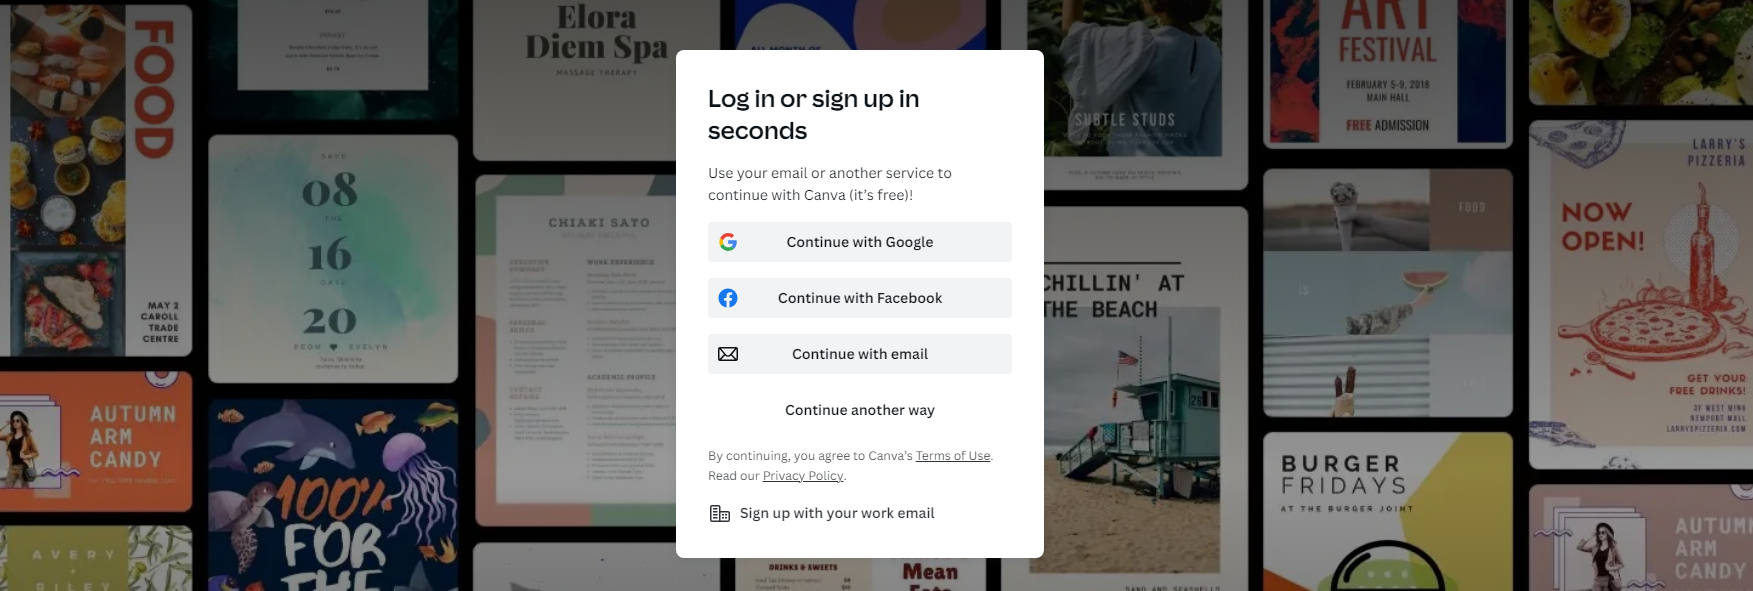
\includegraphics[width=1\textwidth,height=\textheight]{images/clipboard-1368785933.png}}

\hypertarget{navigating-the-canva-interface}{%
\subsubsection*{Navigating the Canva Interface}\label{navigating-the-canva-interface}}
\addcontentsline{toc}{subsubsection}{Navigating the Canva Interface}

The user-centric philosophy of Canva is prominently reflected in its interface design, which prioritizes accessibility and ease of use. The dashboard is strategically organized to facilitate quick and efficient navigation, enabling users to seamlessly transition between different stages of the design process. This section elaborates on the key features of the Canva interface and how they contribute to a streamlined design experience, especially for social media content creation.

\textbf{Dashboard Organization}

Upon logging into Canva, users are greeted by a dashboard that serves as the command center for all design activities. This dashboard is designed with clarity and simplicity in mind, ensuring that users can easily access their ongoing projects, view templates tailored to recent projects, or initiate new designs. The dashboard also provides insights into the latest Canva features and design trends, keeping users informed and inspired.

\begin{itemize}
\tightlist
\item
  \textbf{Quick Start Options}: The dashboard prominently features options for starting a new design, either from scratch or by utilizing Canva's extensive template library. This allows users to quickly embark on new projects without navigating through multiple menus.
\end{itemize}

\textbf{Design Project Selection}

Canva simplifies the process of selecting the right format for social media campaigns by offering a wide range of predefined dimensions, each suited to different platforms and content types. Whether creating an Instagram story, a Facebook banner, or a Twitter post, users can select the appropriate dimensions with just a few clicks, ensuring that their visuals are optimized for each platform's requirements.

\begin{itemize}
\tightlist
\item
  \textbf{Custom Dimensions}: For projects requiring unique dimensions, Canva offers the flexibility to customize the size of the design canvas. This feature is invaluable for creating content that stands out or meets specific criteria not covered by the predefined options.
\end{itemize}

\textbf{The Left-Hand Sidebar: A Gateway to Creativity}

The left-hand sidebar in Canva's interface is a central hub for accessing the platform's vast array of design resources. This sidebar is intuitively categorized, allowing users to effortlessly find and incorporate different elements into their projects.

\begin{itemize}
\tightlist
\item
  \textbf{Templates}: Canva's template library is a treasure trove of professionally designed layouts that span a wide range of themes and styles. Users can filter templates by category or search for specific themes, making it easy to find the perfect starting point for their designs.
\item
  \textbf{Photos and Graphics}: The sidebar provides access to millions of high-quality stock photos and graphics, enabling users to add visual interest and professional polish to their designs. Canva's search function and categorization of these elements make it straightforward to find relevant imagery.
\item
  \textbf{Videos and Audio}: For users looking to create multimedia content, Canva offers a selection of stock videos and audio tracks. These elements can be used to enhance social media posts, advertisements, or presentations, adding a dynamic layer to the visual narrative.
\item
  \textbf{Brand and Team Features}: The sidebar also facilitates brand consistency and collaboration through features like the Brand Kit, where users can store and manage brand-specific elements (colors, logos, fonts), and team collaboration tools, which allow multiple users to work on a project simultaneously.
\end{itemize}

\textbf{Enhancing Social Media Campaigns with Collaboration}

The collaboration features housed within the sidebar underscore Canva's utility for social media campaigns involving multiple stakeholders. Team members can share designs, provide feedback, and make real-time edits, streamlining the campaign development process. This collaborative environment not only fosters creativity but also ensures that the final visuals are aligned with the campaign's objectives and brand standards.

\hypertarget{features-and-tools}{%
\subsection*{Features and Tools}\label{features-and-tools}}
\addcontentsline{toc}{subsection}{Features and Tools}

Canva's suite of features and tools is meticulously designed to cater to the diverse needs of social media content creators. This sub-section explores the key functionalities of Canva that empower users to craft visually appealing and engaging content for social media platforms.

\hypertarget{wide-range-of-templates}{%
\subsubsection*{Wide Range of Templates}\label{wide-range-of-templates}}
\addcontentsline{toc}{subsubsection}{Wide Range of Templates}

Central to Canva's appeal is its extensive collection of templates, which serve as a springboard for creativity. These templates span a myriad of categories including but not limited to social media posts, banners, stories, and advertisements. Each template is thoughtfully designed to align with the dimensions and aesthetic norms of various platforms such as Facebook, Instagram, Twitter, and LinkedIn, ensuring that content creators can deploy platform-optimized visuals with minimal adjustment.

The templates are not only a tool for simplification but also a source of inspiration. They can be fully customized, allowing users to alter colors, fonts, and imagery to suit their branding or campaign theme. This versatility underscores Canva's utility in maintaining brand consistency across multiple social media channels.

\href{https://www.canva.com/templates/}{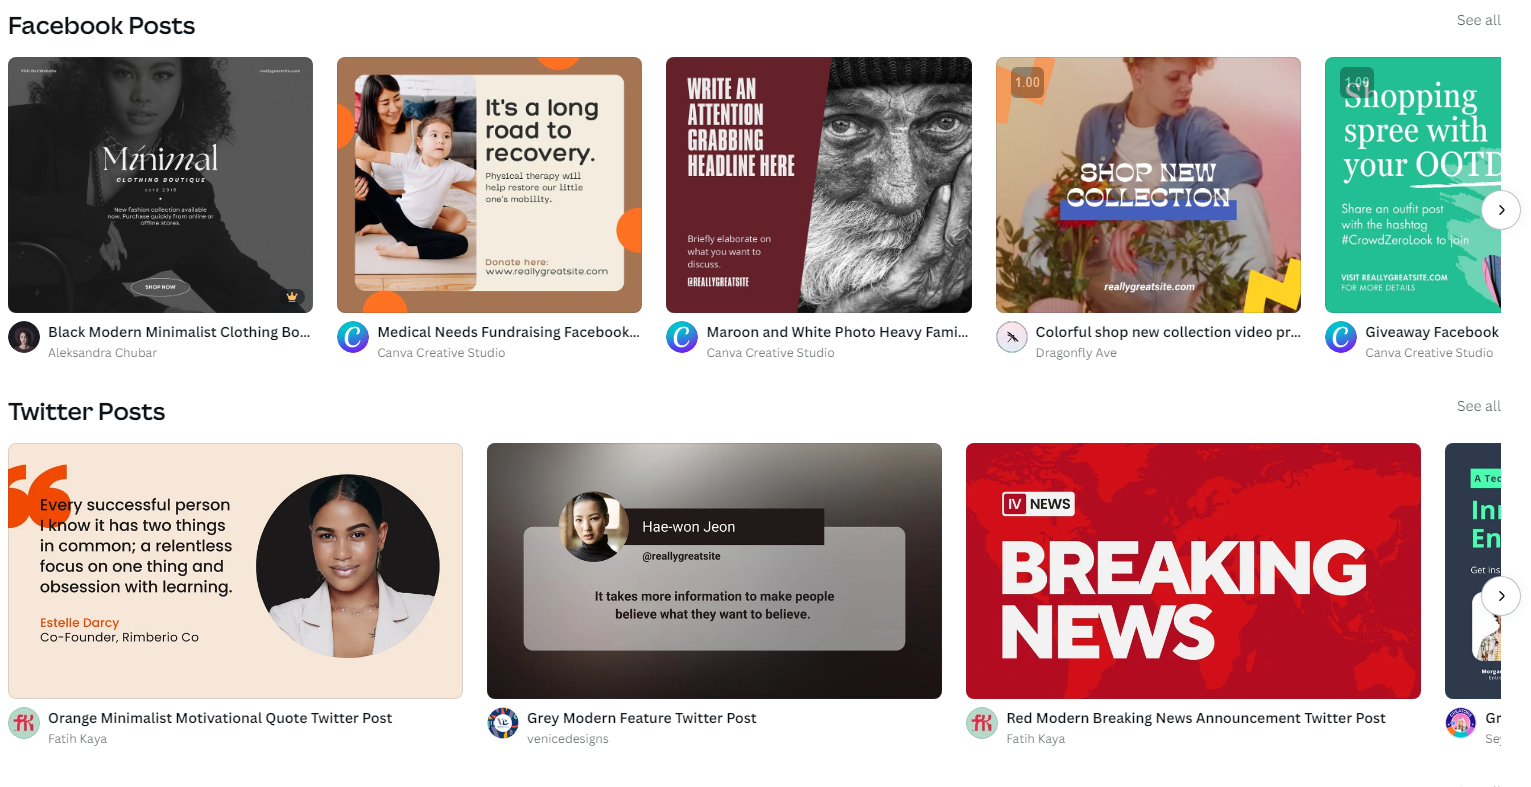
\includegraphics[width=1\textwidth,height=\textheight]{images/clipboard-143261966.png}}

\hypertarget{design-elements}{%
\subsubsection*{Design Elements}\label{design-elements}}
\addcontentsline{toc}{subsubsection}{Design Elements}

Canva's repository of design elements is another cornerstone of its functionality. This repository includes a vast selection of icons, shapes, fonts, and more, enabling users to add depth and personality to their designs. Icons and shapes can be utilized to draw attention to key messages or to add a layer of visual storytelling to the content. The availability of various fonts allows for textual content that is not only readable but also aligned with the brand's tone and personality.

The platform continuously updates its library with new elements, ensuring that users have access to fresh and relevant design assets. This responsiveness to design trends is crucial for social media campaigns, where the ability to stand out in a crowded content landscape can significantly impact engagement rates (Van Dijck, 2013).

\hypertarget{photo-editing-tools}{%
\subsubsection*{Photo Editing Tools}\label{photo-editing-tools}}
\addcontentsline{toc}{subsubsection}{Photo Editing Tools}

High-quality imagery is a critical component of effective social media content. Canva's photo editing tools are robust, offering functionalities ranging from basic cropping and resizing to advanced filters and effects. These tools allow users to enhance their images, ensuring that they are compelling and fit well within the overall design aesthetic.

Canva also offers a feature for background removal, which is particularly useful for creating professional-looking product shots or for layering images in a composite design. Such features are invaluable for creating visually coherent and attention-grabbing social media content.

\hypertarget{utilization-for-various-types-of-social-media-content}{%
\subsubsection*{Utilization for Various Types of Social Media Content}\label{utilization-for-various-types-of-social-media-content}}
\addcontentsline{toc}{subsubsection}{Utilization for Various Types of Social Media Content}

Canva's features and tools are versatile, enabling the creation of a wide array of social media content types. For instance, social media posts and banners can be enriched with Canva's design elements and photo editing tools to capture the audience's attention. Stories, which are designed to be more ephemeral and engaging, can be quickly produced using Canva's templates and customized to fit the brand's narrative.

Advertisements, on the other hand, require a careful balance between visual appeal and message clarity. Canva's templates provide a solid foundation for ad creation, with customization options ensuring that the final product is both compelling and aligned with campaign objectives.

\hypertarget{customization-and-branding}{%
\subsection*{Customization and Branding}\label{customization-and-branding}}
\addcontentsline{toc}{subsection}{Customization and Branding}

A crucial aspect of social media strategy is the establishment and maintenance of a strong, cohesive brand identity. Canva offers a comprehensive suite of features designed to facilitate the customization of designs in a manner that aligns with a brand's identity, ensuring consistency across all social media graphics. This section provides guidance on leveraging Canva's capabilities for branding purposes, focusing on the utilization of brand colors, logos, and fonts.

\hypertarget{establishing-a-brand-kit}{%
\subsubsection*{Establishing a Brand Kit}\label{establishing-a-brand-kit}}
\addcontentsline{toc}{subsubsection}{Establishing a Brand Kit}

Canva's Brand Kit feature is a cornerstone for businesses and individuals aiming to streamline their branding efforts on social media. This feature allows users to upload their logos, set brand colors, and choose fonts that reflect their brand's personality and values. Once established, the Brand Kit becomes a quick reference for all design projects within Canva, enabling the consistent application of visual elements across various types of social media content.

The Brand Kit is particularly beneficial for maintaining uniformity in visual communications. For instance, when creating social media posts, banners, or advertisements, users can instantly apply their brand colors and fonts, thereby reinforcing brand recognition among their audience. This is a premium feature.

\href{https://www.canva.com/pro/brand-kit/}{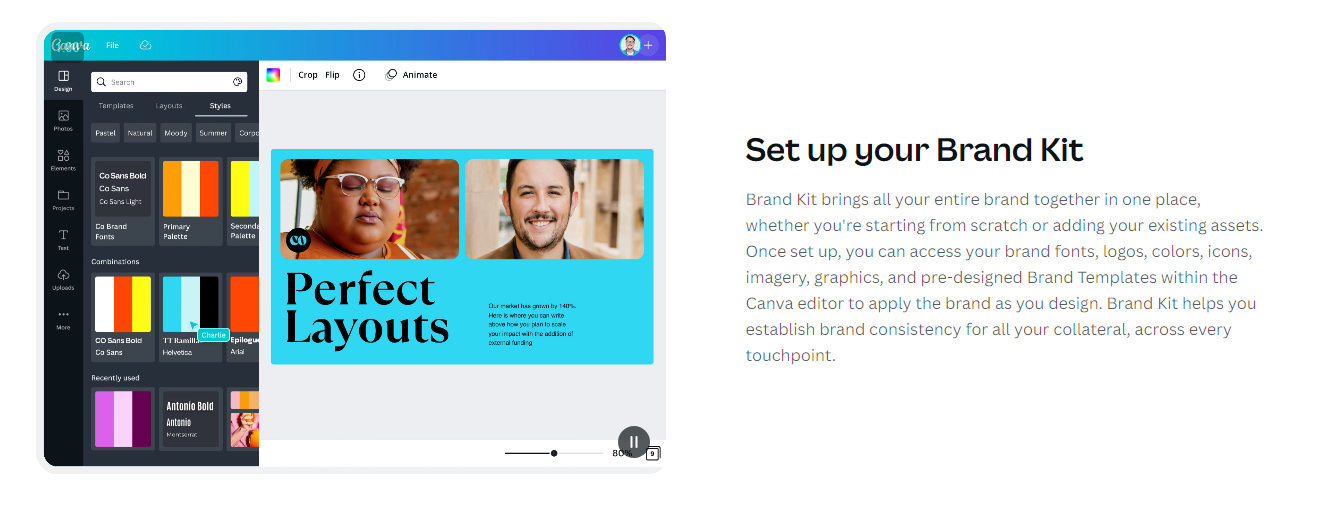
\includegraphics[width=1\textwidth,height=\textheight]{images/clipboard-658121144.png}}

\hypertarget{using-brand-colors}{%
\subsubsection*{Using Brand Colors}\label{using-brand-colors}}
\addcontentsline{toc}{subsubsection}{Using Brand Colors}

Colors play a significant role in brand perception and recognition. Canva allows users to customize the color palette of their designs with precision. By inputting specific color hex codes in the design interface, users can ensure that the colors used in their social media graphics are exactly aligned with their brand colors. This capability is crucial for fostering brand consistency across different platforms and design types.

Furthermore, Canva provides suggestions for color combinations based on the principles of color theory, which can be helpful for users looking to explore complementary colors while staying within the bounds of their brand palette.

\hypertarget{incorporating-logos-and-fonts}{%
\subsubsection*{Incorporating Logos and Fonts}\label{incorporating-logos-and-fonts}}
\addcontentsline{toc}{subsubsection}{Incorporating Logos and Fonts}

Logos are the centerpiece of a brand's visual identity, and Canva simplifies the process of incorporating them into designs. Users can upload their logos into the Brand Kit for easy access and then add them to any design with a few clicks. This ensures that the logo is consistently positioned and sized across all social media graphics, enhancing brand recognition.

Fonts also play a critical role in conveying a brand's voice and personality. Canva's access to a wide range of fonts allows users to select those that best represent their brand. For brands with custom fonts, Canva's Pro version offers the ability to upload these fonts to the Brand Kit, ensuring textual elements in social media graphics are consistent with the brand's overall visual identity.

\hypertarget{collaboration-and-sharing}{%
\subsection*{Collaboration and Sharing}\label{collaboration-and-sharing}}
\addcontentsline{toc}{subsection}{Collaboration and Sharing}

In the dynamic and fast-paced environment of social media campaign planning and execution, the ability to collaborate effectively is paramount. Canva recognizes this need and offers a suite of collaborative features designed to facilitate teamwork and streamline the design process. This section explores how Canva's collaborative features, such as team sharing and real-time editing, can be harnessed to enhance team-based social media campaign efforts.

\hypertarget{team-sharing}{%
\subsubsection*{Team Sharing}\label{team-sharing}}
\addcontentsline{toc}{subsubsection}{Team Sharing}

Canva's team sharing feature is a cornerstone for fostering collaborative work environments. It allows users to create teams within the platform and share designs with team members effortlessly. This functionality is particularly beneficial for social media teams working on a shared campaign, as it enables the seamless exchange of ideas and feedback.

Team members can be invited via email, and once added, they have access to the shared designs and the Brand Kit, ensuring that all team members are aligned with the brand's visual identity standards. This feature supports the maintenance of brand consistency across all social media content, a crucial aspect of effective brand management.

\hypertarget{real-time-editing}{%
\subsubsection*{Real-Time Editing}\label{real-time-editing}}
\addcontentsline{toc}{subsubsection}{Real-Time Editing}

Real-time editing further enhances Canva's collaborative capabilities. Multiple team members can work on a design simultaneously, with changes reflected instantly for all collaborators. This feature is invaluable for social media campaigns, where time is often of the essence, and decisions need to be made quickly.

Real-time feedback and adjustments facilitate a more dynamic and responsive design process. Team members can contribute their expertise and insights, leading to more creative and effective social media graphics. Furthermore, the ability to see edits as they happen reduces the risk of miscommunication and ensures that all team members are on the same page.

\hypertarget{commenting-and-feedback}{%
\subsubsection*{Commenting and Feedback}\label{commenting-and-feedback}}
\addcontentsline{toc}{subsubsection}{Commenting and Feedback}

Canva also includes a commenting feature, allowing team members to leave feedback directly on the design. This tool is crucial for refining designs and ensuring that all elements align with the campaign's objectives. Comments can be addressed, resolved, and revisited, making it easier for teams to track changes and iterations over time.

The integration of direct feedback within the design interface streamlines the review process, reducing the need for external communication tools and enabling more efficient iteration cycles. This aspect of Canva's functionality supports a more cohesive and aligned team effort in social media campaign development.

\hypertarget{access-and-permissions-management}{%
\subsubsection*{Access and Permissions Management}\label{access-and-permissions-management}}
\addcontentsline{toc}{subsubsection}{Access and Permissions Management}

To further support collaboration, Canva allows for the management of access and permissions within teams. Administrators can control who has the ability to edit, view, or comment on specific designs. This granularity in permissions ensures that sensitive or critical design elements are protected, while still promoting a collaborative workspace.

This level of control is especially important in larger teams or organizations where different members may have varying roles in the social media campaign process. By precisely managing access and permissions, teams can maintain a balance between collaboration and control, ensuring that the integrity of the brand and campaign is preserved.

\hypertarget{design-principles-for-social-media-visuals}{%
\section{Design Principles for Social Media Visuals}\label{design-principles-for-social-media-visuals}}

\hypertarget{understanding-design-basics}{%
\subsection*{Understanding Design Basics}\label{understanding-design-basics}}
\addcontentsline{toc}{subsection}{Understanding Design Basics}

The creation of effective social media visuals is not solely reliant on artistic talent; it fundamentally rests on the application of core design principles. These principles---balance, contrast, hierarchy, alignment, and repetition---are critical in crafting visuals that are not only aesthetically pleasing but also strategically optimized for engagement and communication. This section delves into these foundational design principles, illustrating how they contribute to the creation of compelling social media content.

\hypertarget{balance}{%
\subsubsection*{Balance}\label{balance}}
\addcontentsline{toc}{subsubsection}{Balance}

Balance in design refers to the distribution of visual weight across a layout. It can be achieved symmetrically, where elements are mirrored on either side of a central axis, or asymmetrically, where different elements achieve visual equilibrium through contrast in size, color, or texture. In social media visuals, balance is key to creating a sense of stability and harmony, making the content more visually appealing and easier to digest. For example, a balanced layout can ensure that no single element overwhelms the others, allowing the viewer's eye to move smoothly across the content.

\hypertarget{contrast}{%
\subsubsection*{Contrast}\label{contrast}}
\addcontentsline{toc}{subsubsection}{Contrast}

Contrast involves the juxtaposition of differing elements (such as color, shape, or size) to create visual interest and draw attention. In the context of social media, contrast can be a powerful tool to highlight important information, guide viewers' attention to calls to action, or make key messages stand out. Effective use of contrast ensures that visuals are not only eye-catching but also effectively communicate the intended message.

\href{https://www.zekagraphic.com/visual-hierarchy-graphic-design-principles/}{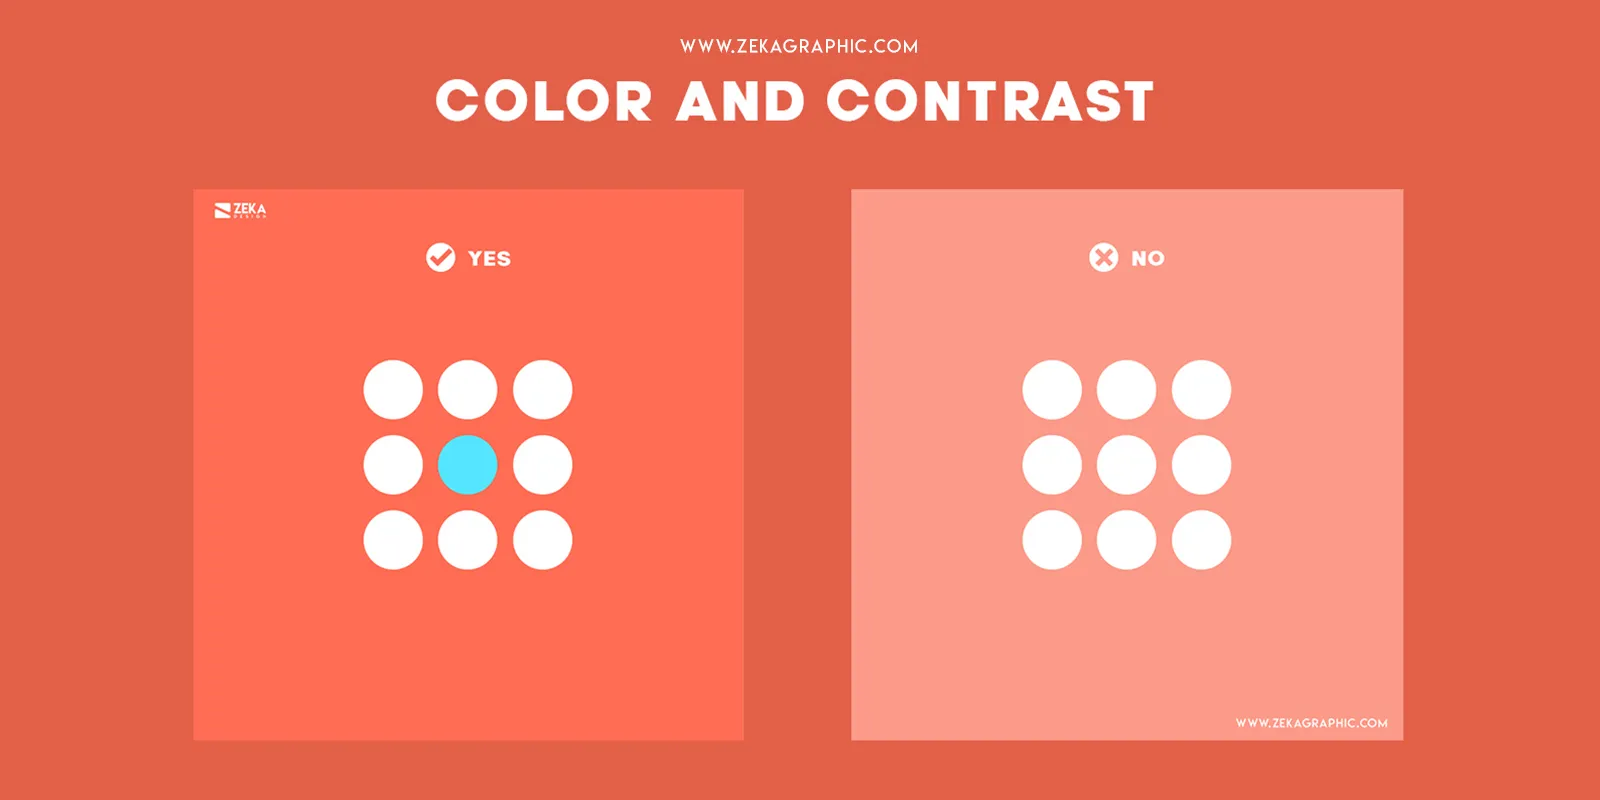
\includegraphics[width=1\textwidth,height=\textheight]{images/clipboard-2970953759.png}}

\hypertarget{hierarchy}{%
\subsubsection*{Hierarchy}\label{hierarchy}}
\addcontentsline{toc}{subsubsection}{Hierarchy}

Visual hierarchy refers to the arrangement of elements in a way that implies importance, guiding the viewer's attention through the content in a deliberate manner. By manipulating size, color, positioning, and other design elements, designers can direct viewers' eyes to the most critical information first. In social media visuals, establishing a clear hierarchy is essential for ensuring that key messages are seen and understood quickly, given the fleeting nature of users' attention spans online.

\href{https://www.zekagraphic.com/visual-hierarchy-graphic-design-principles/}{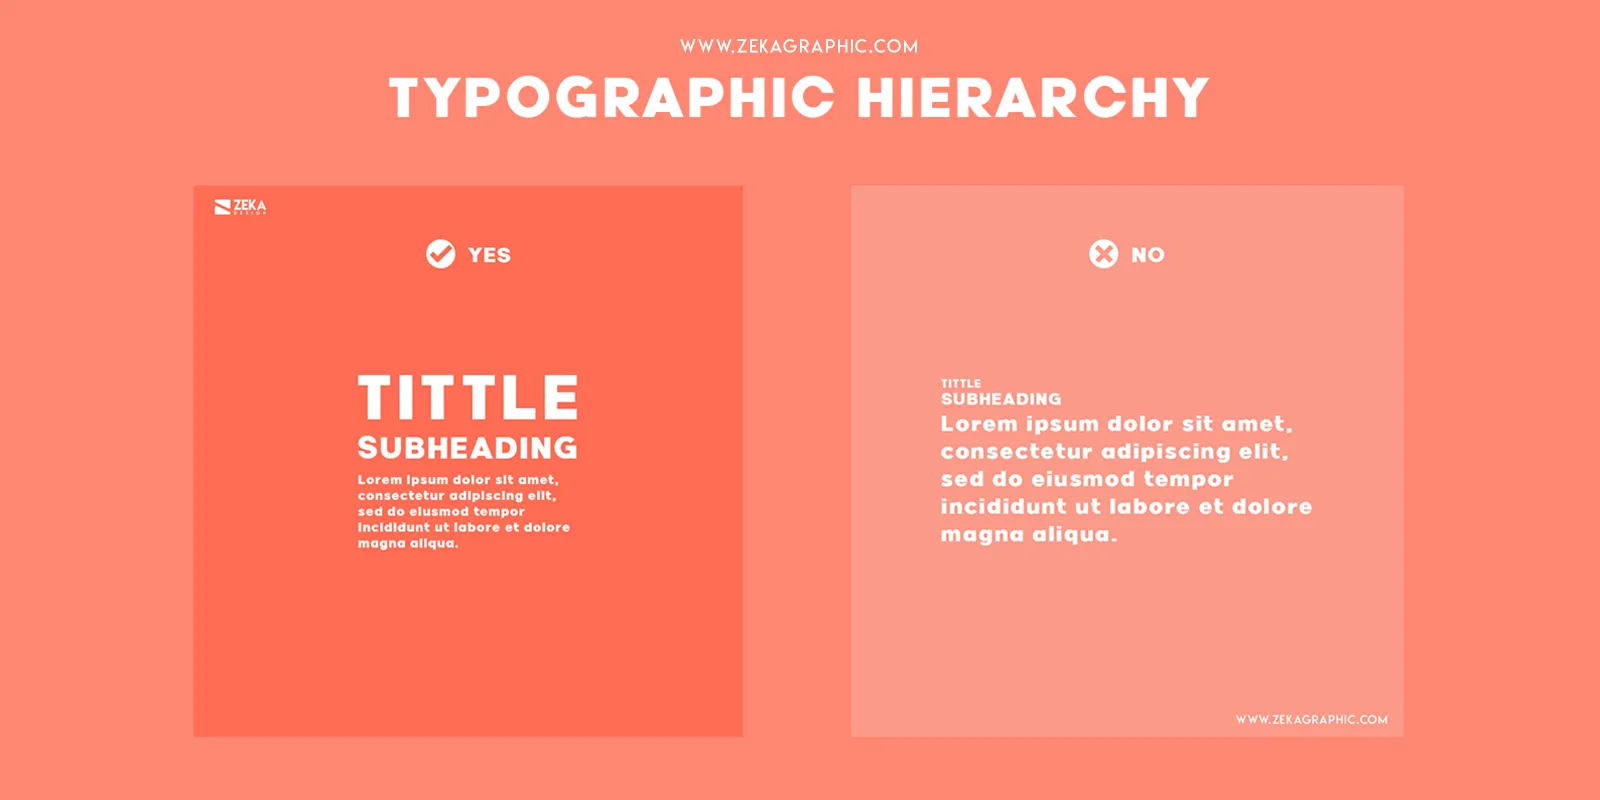
\includegraphics[width=1\textwidth,height=\textheight]{images/clipboard-3530120539.png}}

\hypertarget{alignment}{%
\subsubsection*{Alignment}\label{alignment}}
\addcontentsline{toc}{subsubsection}{Alignment}

Alignment is the principle of organizing elements in a layout so that their edges or axes line up along common rows, columns, or centers. This principle is crucial for creating a sense of order and coherence in social media visuals. Proper alignment not only enhances the readability of content but also contributes to a sleek, professional appearance, reinforcing the credibility of the message.

\href{https://www.zekagraphic.com/visual-hierarchy-graphic-design-principles/}{
\includegraphics[width=1\textwidth,height=\textheight]{images/clipboard-3373048530.png}}

\hypertarget{repetition}{%
\subsubsection*{Repetition}\label{repetition}}
\addcontentsline{toc}{subsubsection}{Repetition}

Repetition involves the consistent use of specific design elements, such as colors, fonts, or shapes, across a series of visuals. This principle is integral to branding, as it helps to create a recognizable and memorable visual identity for a brand or campaign. On social media, repetition strengthens brand recognition and fosters a sense of familiarity and trust among the audience.

\href{https://www.zekagraphic.com/visual-hierarchy-graphic-design-principles/}{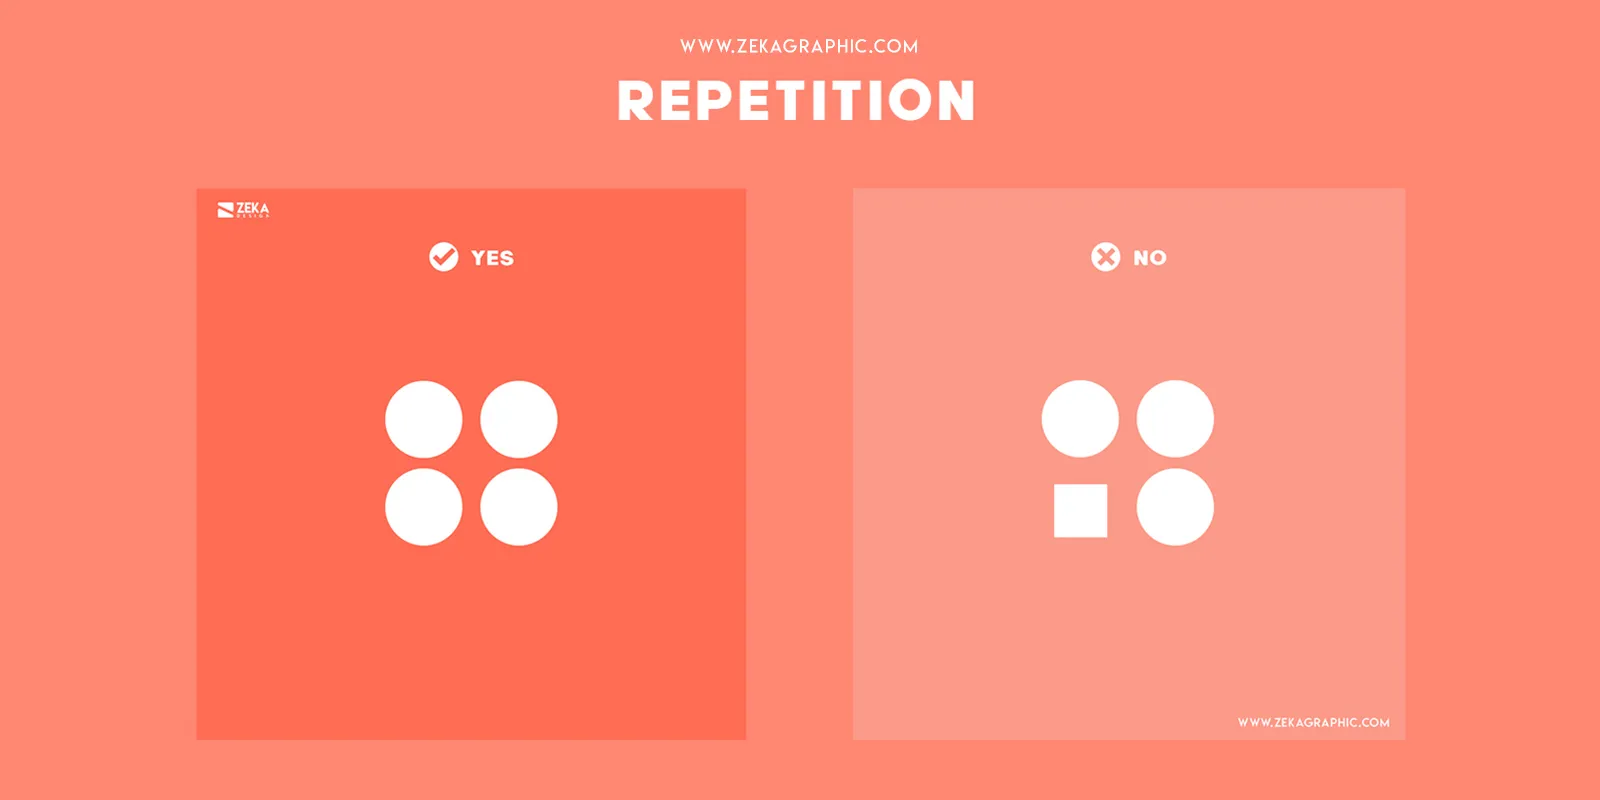
\includegraphics[width=1\textwidth,height=\textheight]{images/clipboard-2425648746.png}}

\hypertarget{designing-for-different-platforms}{%
\subsection*{Designing for Different Platforms}\label{designing-for-different-platforms}}
\addcontentsline{toc}{subsection}{Designing for Different Platforms}

The landscape of social media is characterized by its diversity, with each platform possessing its own unique formats, functionalities, and audience expectations. This variation necessitates a tailored approach to design, where best practices and requirements are adapted to suit the specific nuances of each platform. This section explores the distinctive design considerations for popular social media platforms---Instagram, Facebook, Twitter, and LinkedIn---and offers guidance on optimizing visual content to engage effectively with the respective audiences of each platform.

\hypertarget{instagram-1}{%
\subsubsection*{Instagram}\label{instagram-1}}
\addcontentsline{toc}{subsubsection}{Instagram}

Instagram is a visually driven platform, with a primary focus on high-quality images and videos. Design for Instagram should prioritize vibrant, eye-catching visuals that can stand out in a highly competitive feed. Given its mobile-first nature, content should be optimized for viewing on smartphones, with emphasis on simplicity and clarity. Instagram Stories and Reels offer additional formats for creative expression, requiring designs that are engaging and can convey messages quickly. The use of hashtags and location tags in visuals can also enhance discoverability.

\href{https://www.canva.com/instagram-stories/templates/}{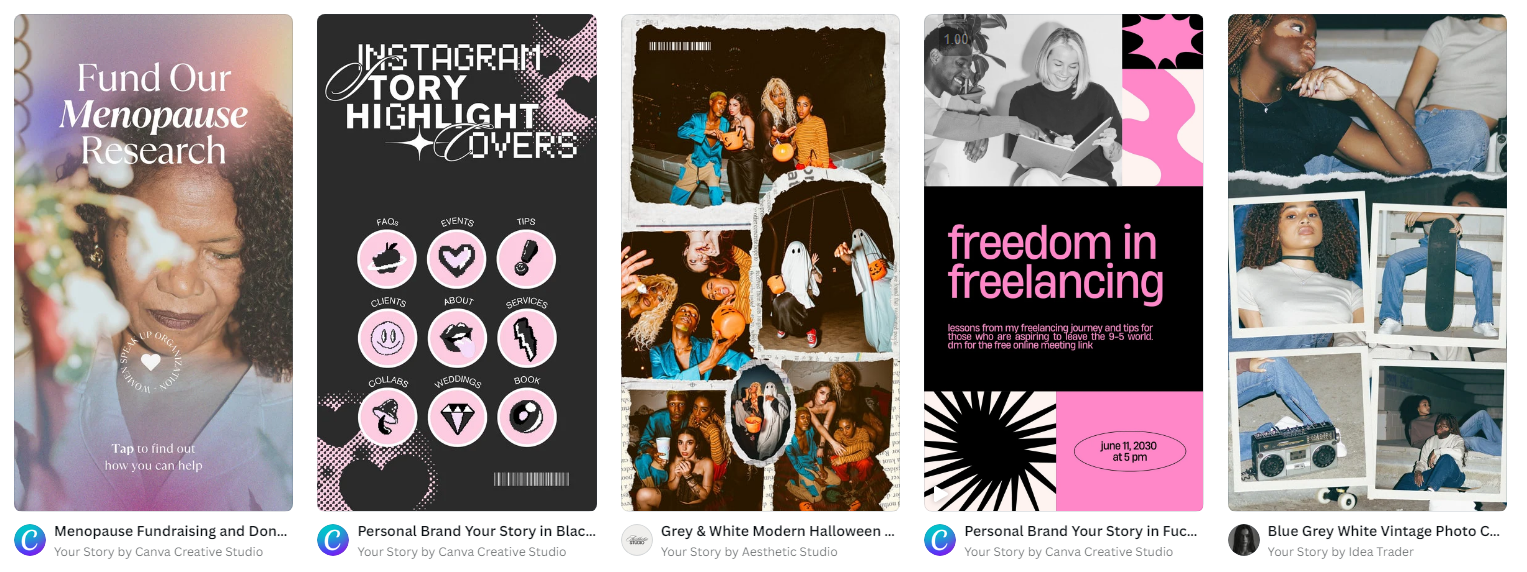
\includegraphics[width=1\textwidth,height=\textheight]{images/clipboard-2708767155.png}}

\hypertarget{facebook-1}{%
\subsubsection*{Facebook}\label{facebook-1}}
\addcontentsline{toc}{subsubsection}{Facebook}

Facebook supports a wide range of content types, including images, videos, links, and text-based posts. Design for Facebook should account for the platform's diverse audience and the potential for content to be shared beyond the immediate followers. Images and videos should be designed to convey the message even without sound or accompanying text, considering that many users scroll through their feed with audio off. Additionally, attention should be paid to how visuals accompany shared links, ensuring that thumbnails are engaging and representative of the content.

\href{https://www.canva.com/facebook-posts/templates/}{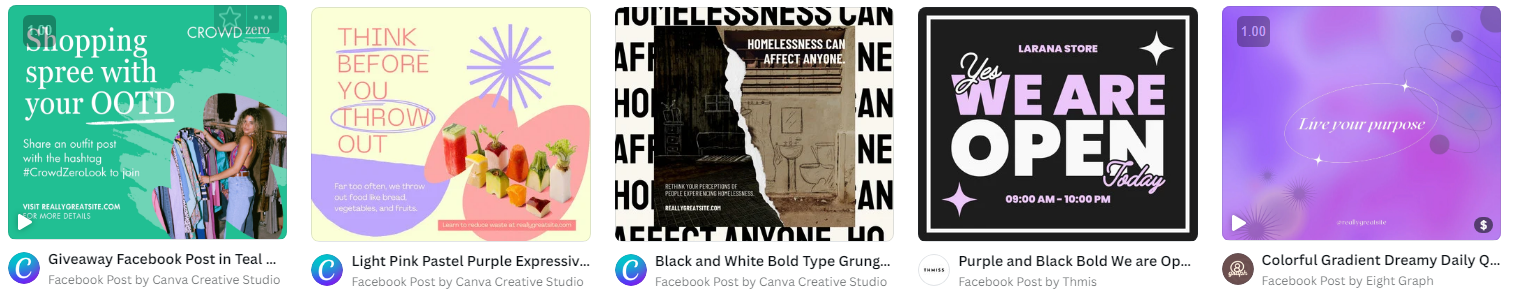
\includegraphics[width=1\textwidth,height=\textheight]{images/clipboard-1380762122.png}}

\hypertarget{twitter-1}{%
\subsubsection*{Twitter}\label{twitter-1}}
\addcontentsline{toc}{subsubsection}{Twitter}

Twitter's fast-paced, text-centric nature does not diminish the value of visuals; instead, it highlights the need for designs that can capture attention quickly. Images, GIFs, and videos should complement the concise text, making tweets more noticeable. Given Twitter's character limit, visuals serve as an essential tool for extending the message. Designs for Twitter should be straightforward and focused, with clear call-to-actions when applicable. The platform's real-time nature also calls for timely and topical content, which can involve adapting designs to current events or trends.

\href{https://www.canva.com/twitter/templates/posts/}{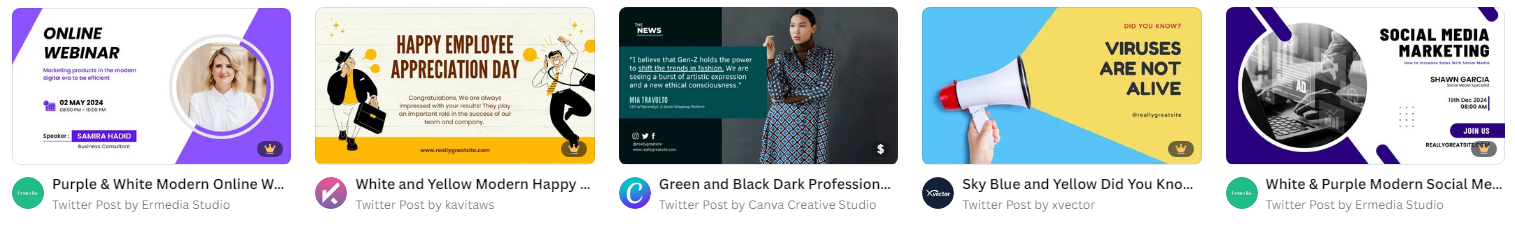
\includegraphics[width=1\textwidth,height=\textheight]{images/clipboard-2219953613.png}}

\hypertarget{linkedin-1}{%
\subsubsection*{LinkedIn}\label{linkedin-1}}
\addcontentsline{toc}{subsubsection}{LinkedIn}

LinkedIn's professional context influences its design best practices significantly. Visual content should project a professional image, with a focus on supporting business and career-related objectives. Infographics, charts, and professional photos can enhance posts, making them more engaging to the platform's audience. Designing for LinkedIn also involves consideration of how visuals contribute to personal or organizational branding, with a preference for content that adds value or insight into industry-specific discussions.

\href{https://www.canva.com/linkedin-posts/templates/}{
\includegraphics[width=1\textwidth,height=\textheight]{images/clipboard-2317314021.png}}

\hypertarget{use-of-color-and-typography}{%
\subsection*{Use of Color and Typography}\label{use-of-color-and-typography}}
\addcontentsline{toc}{subsection}{Use of Color and Typography}

The strategic selection of color schemes and typography is crucial in crafting effective social media visuals. These elements play a significant role in conveying mood, establishing tone, and ensuring the readability of content. This section provides detailed guidance on the use of color and typography, incorporating insights from color psychology and font pairing best practices to enhance the impact of social media designs.

\hypertarget{color-psychology-in-social-media-design}{%
\subsubsection*{Color Psychology in Social Media Design}\label{color-psychology-in-social-media-design}}
\addcontentsline{toc}{subsubsection}{Color Psychology in Social Media Design}

Color psychology explores how different colors influence human behavior and emotional responses. In the context of social media, colors can be used to evoke specific emotions, attract attention, and even influence decision-making processes. For instance, blue is often associated with trust and reliability, making it a popular choice for brands aiming to establish a sense of security. Red, on the other hand, is associated with excitement and urgency, which can be leveraged in calls to action or promotional content (Elliot \& Maier, 2014).

When selecting a color scheme for social media visuals, it is important to consider the brand's identity and the emotions or actions the content is intended to evoke. Additionally, the use of contrasting colors can improve readability and highlight key elements, while a harmonious color palette can create a visually pleasing and cohesive look.

\hypertarget{typography-and-readability}{%
\subsubsection*{Typography and Readability}\label{typography-and-readability}}
\addcontentsline{toc}{subsubsection}{Typography and Readability}

Typography---the art of arranging type---plays a pivotal role in the readability and overall aesthetic of social media content. The choice of font should align with the brand's personality while ensuring that text is legible across different devices and screen sizes. Sans-serif fonts, for example, are often preferred for digital platforms due to their clarity and simplicity, making them easy to read even at smaller sizes (Wheeler, 2012).

Font pairing, or the combination of complementary fonts, can add visual interest and hierarchy to content. A common practice is to pair a bold, attention-grabbing font for headlines with a simpler, more readable font for body text. This not only enhances the visual appeal of the design but also guides the viewer's attention to key messages.

\hypertarget{tips-for-effective-use-of-color-and-typography}{%
\subsubsection*{Tips for Effective Use of Color and Typography}\label{tips-for-effective-use-of-color-and-typography}}
\addcontentsline{toc}{subsubsection}{Tips for Effective Use of Color and Typography}

\begin{itemize}
\tightlist
\item
  \textbf{Understand the target audience}: Different demographics may respond differently to color schemes and typographic styles. Consider the preferences and expectations of the target audience when designing social media visuals.
\item
  \textbf{Ensure accessibility}: Choose color combinations and font sizes that are accessible to people with visual impairments. Tools like contrast checkers can help ensure that text is legible against its background.
\item
  \textbf{Maintain brand consistency}: Use colors and fonts that are aligned with the brand's existing visual identity. This reinforces brand recognition and ensures a cohesive presence across all social media platforms.
\item
  \textbf{Experiment with trends cautiously}: While it's important to stay current, ensure that any trendy color schemes or fonts do not compromise the brand's identity or the content's readability.
\end{itemize}

\hypertarget{visual-content-strategy}{%
\subsection*{Visual Content Strategy}\label{visual-content-strategy}}
\addcontentsline{toc}{subsection}{Visual Content Strategy}

A comprehensive visual content strategy is instrumental in forging a cohesive brand identity across various social media platforms. This strategy encompasses the deliberate planning, creation, and distribution of visuals that consistently reflect the brand's core values, aesthetics, and messaging. The significance of a visual content strategy lies not only in maintaining uniformity in visual branding but also in enhancing brand recognition and facilitating deeper audience engagement. This section elucidates the components of a visual content strategy and its pivotal role in social media marketing.

\hypertarget{establishing-a-unified-visual-identity}{%
\subsubsection*{Establishing a Unified Visual Identity}\label{establishing-a-unified-visual-identity}}
\addcontentsline{toc}{subsubsection}{Establishing a Unified Visual Identity}

The cornerstone of an effective visual content strategy is the establishment of a unified visual identity. This identity is a composite of the brand's color palette, typography, imagery, and logo usage, which together create a distinctive look and feel that is instantly recognizable to the audience. Consistency in these visual elements across all touchpoints reinforces brand recall, making it easier for the audience to identify the brand's content amidst the plethora of information on social media (Aaker, 1996).

A unified visual identity also conveys professionalism and credibility, fostering trust among the audience. Tools like Canva's Brand Kit facilitate the implementation of this consistency by providing a centralized repository for brand elements, ensuring that every piece of content aligns with the brand's visual standards.

\hypertarget{tailoring-content-for-platform-specificities}{%
\subsubsection*{Tailoring Content for Platform Specificities}\label{tailoring-content-for-platform-specificities}}
\addcontentsline{toc}{subsubsection}{Tailoring Content for Platform Specificities}

While consistency is key, a nuanced understanding of the unique formats and audience expectations of different social media platforms is equally crucial. Each platform has its own set of norms and best practices for visual content. For instance, Instagram favors high-quality, aesthetically pleasing images and videos, while LinkedIn content may require a more professional and polished approach. Tailoring content to align with these specificities, without compromising the brand's visual identity, optimizes engagement on each platform and enhances overall brand presence (Smith, 2020).

\hypertarget{fostering-engagement-through-visual-storytelling}{%
\subsubsection*{Fostering Engagement through Visual Storytelling}\label{fostering-engagement-through-visual-storytelling}}
\addcontentsline{toc}{subsubsection}{Fostering Engagement through Visual Storytelling}

Visual storytelling is a powerful component of a visual content strategy, capable of evoking emotions and building a narrative around the brand. By crafting visuals that tell a story---whether it's the journey of a product from conception to market, the impact of services on customers, or the brand's commitment to certain values---brands can create a more immersive and engaging experience for their audience. This storytelling approach not only enhances the memorability of the content but also encourages sharing, further extending the brand's reach and engagement levels (Jenkins, 2006).

\hypertarget{measuring-and-adapting-the-strategy}{%
\subsubsection*{Measuring and Adapting the Strategy}\label{measuring-and-adapting-the-strategy}}
\addcontentsline{toc}{subsubsection}{Measuring and Adapting the Strategy}

An effective visual content strategy is not static; it requires ongoing measurement and adaptation. Key performance indicators (KPIs) such as engagement rates, click-through rates, and conversion rates can provide insights into the effectiveness of the visual content. Regular analysis of these metrics allows brands to refine their strategy, experimenting with new visual trends, formats, and messaging to better resonate with their audience. This adaptive approach ensures that the visual content strategy remains aligned with changing audience preferences and platform algorithms, sustaining the brand's relevance and engagement over time.

\hypertarget{creating-engaging-content-with-canva}{%
\section{Creating Engaging Content with Canva}\label{creating-engaging-content-with-canva}}

\hypertarget{developing-engaging-designs}{%
\subsection*{Developing Engaging Designs}\label{developing-engaging-designs}}
\addcontentsline{toc}{subsection}{Developing Engaging Designs}

In the dynamic realm of social media, the ability to create content that captivates and encourages sharing is invaluable. Canva, with its comprehensive suite of design tools and resources, serves as a powerful ally in this endeavor. This section provides actionable tips and techniques for leveraging Canva to develop engaging and shareable social media content, focusing on the effective use of templates, graphic elements, and Canva's extensive photo library.

\hypertarget{leveraging-templates-for-professional-designs}{%
\subsubsection*{Leveraging Templates for Professional Designs}\label{leveraging-templates-for-professional-designs}}
\addcontentsline{toc}{subsubsection}{Leveraging Templates for Professional Designs}

Canva's vast array of templates is a significant asset for content creators aiming to produce professional and engaging designs quickly. These templates, which range from social media posts and stories to advertisements and infographics, provide a solid foundation upon which users can build and customize their content. To maximize the effectiveness of these templates, consider the following:

\begin{itemize}
\tightlist
\item
  \textbf{Select Templates Aligned with Brand Identity}: Choose templates that reflect your brand's visual style and values. Consistency in visuals reinforces brand recognition among your audience.
\item
  \textbf{Customize to Stand Out}: While templates offer a starting point, customization is key to creating unique content. Adjust colors, fonts, and imagery to tailor the design to your message and audience preferences.
\item
  \textbf{Use Templates as Inspiration}: Even if you decide not to use a template directly, browsing through Canva's collection can spark creative ideas and help you identify design trends that resonate with your target audience.
\end{itemize}

\hypertarget{incorporating-graphic-elements-for-visual-interest}{%
\subsubsection*{Incorporating Graphic Elements for Visual Interest}\label{incorporating-graphic-elements-for-visual-interest}}
\addcontentsline{toc}{subsubsection}{Incorporating Graphic Elements for Visual Interest}

Graphic elements, including icons, shapes, and illustrations, can add depth and visual interest to your designs, making them more engaging and shareable. Canva offers a wide range of graphic elements that can be used to enhance your content:

\begin{itemize}
\tightlist
\item
  \textbf{Highlight Key Messages with Icons and Shapes}: Use icons and shapes to draw attention to important information or to complement your content's theme.
\item
  \textbf{Balance Composition}: Integrate graphic elements thoughtfully to balance your design's composition, ensuring that it remains visually appealing without overwhelming the message.
\item
  \textbf{Create Visual Hierarchy}: Use size and placement of graphic elements to establish a visual hierarchy, guiding the viewer's eye to the most critical parts of your message.
\end{itemize}

\hypertarget{utilizing-canvas-photo-library-for-high-quality-imagery}{%
\subsubsection*{Utilizing Canva's Photo Library for High-Quality Imagery}\label{utilizing-canvas-photo-library-for-high-quality-imagery}}
\addcontentsline{toc}{subsubsection}{Utilizing Canva's Photo Library for High-Quality Imagery}

High-quality, relevant imagery is crucial for engaging social media content. Canva's extensive photo library provides access to millions of high-resolution images that can be used to enhance your designs:

\begin{itemize}
\tightlist
\item
  \textbf{Select Relevant, High-Quality Images}: Choose images that are not only of high quality but also relevant to your content's message and audience's interests.
\item
  \textbf{Edit for Consistency}: Utilize Canva's photo editing tools to adjust brightness, contrast, and saturation to ensure that the images fit seamlessly with your overall design and brand aesthetic.
\item
  \textbf{Incorporate Branding}: When appropriate, add your logo or brand colors to images, reinforcing brand identity and increasing brand recognition across social media channels.
\end{itemize}

\hypertarget{interactive-and-animated-features}{%
\subsection*{Interactive and Animated Features}\label{interactive-and-animated-features}}
\addcontentsline{toc}{subsection}{Interactive and Animated Features}

In the evolving landscape of social media, dynamic content such as animations and interactive features play a pivotal role in capturing audience attention and enhancing engagement. Canva provides a versatile suite of tools designed to create such content, enabling users to craft animated posts, video stories, and other interactive visuals with ease. This section offers detailed guidance on harnessing Canva's interactive and animated features to produce content that stands out on platforms like Instagram, Facebook, and beyond.

\hypertarget{leveraging-animation}{%
\subsubsection*{Leveraging Animation}\label{leveraging-animation}}
\addcontentsline{toc}{subsubsection}{Leveraging Animation}

Animation can transform static images into engaging pieces of content, adding a layer of depth and movement that captures and retains the viewer's attention. Canva offers a range of animation options for text and graphic elements, from subtle movements to more pronounced effects. These animations can be applied to individual elements or the entire design, depending on the desired impact.

When incorporating animation, it's important to consider the context and platform. For instance, subtle animations may be more appropriate for professional platforms like LinkedIn, while more vibrant animations can be effective on Instagram or Twitter. Animated posts can be used for a variety of purposes, from highlighting key messages in a campaign to creating visually engaging announcements or updates.

\hypertarget{creating-video-stories}{%
\subsubsection*{Creating Video Stories}\label{creating-video-stories}}
\addcontentsline{toc}{subsubsection}{Creating Video Stories}

Video stories have become a staple on platforms such as Instagram, Facebook, and Snapchat, offering a dynamic way to share content that engages users with short, compelling narratives. Canva's video story templates and drag-and-drop interface simplify the process of creating professional-looking video content. Users can select from a vast library of stock videos or upload their own footage, then customize the videos with text, music, and other elements to fit their campaign's needs.

For effective video stories, it's crucial to craft a narrative that resonates with the audience, whether it's informative, inspirational, or entertaining. Incorporating branded elements such as logos and color schemes ensures consistency and reinforces brand identity.

\hypertarget{utilizing-interactive-features}{%
\subsubsection*{Utilizing Interactive Features}\label{utilizing-interactive-features}}
\addcontentsline{toc}{subsubsection}{Utilizing Interactive Features}

Beyond animations and videos, Canva supports the creation of interactive content, such as clickable social media posts and infographics. These features can significantly enhance user engagement by encouraging active participation. For example, interactive infographics created in Canva can be used to present data in a more engaging manner, with clickable elements revealing additional information or related content.

Interactive posts can also direct traffic to a website or landing page, serving as an effective tool for conversion within a broader social media strategy. Ensuring that the call to action (CTA) is clear and compelling is key to maximizing the effectiveness of interactive content.

\hypertarget{best-practices-for-dynamic-content-creation}{%
\subsubsection*{Best Practices for Dynamic Content Creation}\label{best-practices-for-dynamic-content-creation}}
\addcontentsline{toc}{subsubsection}{Best Practices for Dynamic Content Creation}

\begin{itemize}
\tightlist
\item
  \textbf{Keep the message clear}: Ensure that the use of animations or interactive elements does not obscure the key message. The content should be engaging but not overwhelming.
\item
  \textbf{Optimize for loading times}: Be mindful of file sizes, particularly for animated and video content, to ensure quick loading times and a smooth user experience across all devices.
\item
  \textbf{Test across platforms}: Different social media platforms may display animated and interactive content differently. Testing content across platforms ensures compatibility and optimal presentation.
\item
  \textbf{Monitor engagement}: Use social media analytics to track the performance of dynamic content, gaining insights into what resonates with the audience and refining strategies accordingly.
\end{itemize}

\hypertarget{optimizing-visuals-for-engagement}{%
\subsection*{Optimizing Visuals for Engagement}\label{optimizing-visuals-for-engagement}}
\addcontentsline{toc}{subsection}{Optimizing Visuals for Engagement}

In the realm of social media, where content saturation is high, optimizing visuals for engagement is not just beneficial---it's essential. Engaging visuals can significantly increase the likelihood of user interaction, from likes and shares to comments and conversions. This section focuses on best practices for optimizing visuals to enhance user engagement, covering critical aspects such as size specifications for different platforms, text readability, and the strategic use of calls-to-action (CTAs).

\hypertarget{size-specifications-for-different-platforms}{%
\subsubsection*{Size Specifications for Different Platforms}\label{size-specifications-for-different-platforms}}
\addcontentsline{toc}{subsubsection}{Size Specifications for Different Platforms}

Each social media platform has its own set of size specifications for images and videos, designed to ensure optimal display and user experience. Adhering to these specifications is crucial for preventing issues such as cropping or distortion, which can detract from the visual's impact and the message's clarity.

\begin{itemize}
\tightlist
\item
  \textbf{Instagram}: Offers various formats, including square (1080px by 1080px), portrait (1080px by 1350px), and landscape (1080px by 566px). Stories and reels require 1080px by 1920px for full-screen vertical display.
\item
  \textbf{Facebook}: Recommends 1200px by 630px for shared images and 1080px by 1920px for stories to ensure clear display in the news feed and full-screen in stories.
\item
  \textbf{Twitter}: Suggests a 16:9 aspect ratio for images and videos, with a minimum size of 600px by 335px for images to avoid stretching in the feed.
\item
  \textbf{LinkedIn}: Prefers 1200px by 627px for standard posts, ensuring visuals are tailored for a professional audience's desktop and mobile viewing.
\end{itemize}

These specifications are subject to change; regularly consulting platform guidelines is advisable to stay current.

\hypertarget{ensuring-text-readability}{%
\subsubsection*{Ensuring Text Readability}\label{ensuring-text-readability}}
\addcontentsline{toc}{subsubsection}{Ensuring Text Readability}

Text within visuals plays a pivotal role in conveying messages and inducing action. Ensuring text readability is thus paramount. This involves selecting fonts and sizes that are easily legible across devices and contrasting text color with the background to enhance visibility. Canva offers features like text spacing and opacity adjustments, enabling finer control over text presentation.

\begin{itemize}
\tightlist
\item
  \textbf{Contrast and Color}: Use high-contrast color combinations for text and backgrounds to ensure readability.
\item
  \textbf{Font Size and Style}: Opt for larger font sizes and clear, simple font styles to improve legibility, especially on mobile devices where screen real estate is limited.
\end{itemize}

\hypertarget{incorporating-calls-to-action-ctas}{%
\subsubsection*{Incorporating Calls-to-Action (CTAs)}\label{incorporating-calls-to-action-ctas}}
\addcontentsline{toc}{subsubsection}{Incorporating Calls-to-Action (CTAs)}

A well-placed CTA within a visual can significantly increase engagement by guiding users on the next steps, whether it's to share the content, visit a website, or participate in a survey. CTAs should be concise, compelling, and visually distinct, making it clear what action the user is expected to take.

\begin{itemize}
\tightlist
\item
  \textbf{Visibility}: Place CTAs in a prominent position within the visual, ensuring they are easily noticeable.
\item
  \textbf{Design}: Use buttons or contrasting colors to make CTAs stand out from the rest of the visual content.
\item
  \textbf{Message}: Craft CTA messages that convey urgency or value to encourage immediate action, such as ``Learn more,'' ``Sign up today,'' or ``Join the conversation.''
\end{itemize}

\hypertarget{setting-smart-goals-for-social-media-campaigns}{%
\chapter{Setting SMART Goals for Social Media Campaigns}\label{setting-smart-goals-for-social-media-campaigns}}

\hypertarget{principles-of-smart-goals}{%
\section*{Principles of SMART Goals}\label{principles-of-smart-goals}}
\addcontentsline{toc}{section}{Principles of SMART Goals}

The chapter on ``Setting SMART Goals for Social Media Campaigns'' plays a crucial role in preparing students for the challenges and opportunities of social media analytics within the landscape of digital marketing. This chapter aims to provide an in-depth exploration of the principles of SMART goals, a framework that is indispensable for crafting effective and strategic objectives for social media initiatives. By understanding and applying these principles, students will be better equipped to design, implement, and measure successful social media campaigns that are aligned with broader marketing and organizational goals.

\hypertarget{introduction-to-smart-goals}{%
\subsection*{Introduction to SMART Goals}\label{introduction-to-smart-goals}}
\addcontentsline{toc}{subsection}{Introduction to SMART Goals}

The introduction of the SMART framework is foundational to the establishment of clear, achievable, and quantifiable goals, which are essential for the success of social media campaigns. The acronym SMART stands for Specific, Measurable, Achievable, Relevant, and Time-bound. Each of these criteria serves a distinct purpose in enhancing the effectiveness and practicality of goals. This section underlines the critical importance of the SMART framework in creating objectives that are not only actionable but also integral to the strategic planning of social media campaigns, providing a solid foundation for students to develop their planning and execution skills.

\hypertarget{breaking-down-the-smart-acronym}{%
\subsection*{Breaking Down the SMART Acronym}\label{breaking-down-the-smart-acronym}}
\addcontentsline{toc}{subsection}{Breaking Down the SMART Acronym}

The section ``Breaking Down the SMART Acronym'' within the chapter titled ``Setting SMART Goals for Social Media Campaigns'' is pivotal in equipping students with the analytical skills needed to navigate the complexities of social media analytics effectively. This expanded breakdown delves into the nuances of each aspect of the SMART framework, offering a comprehensive guide to crafting precise, actionable goals tailored to the unique dynamics of social media platforms.

\hypertarget{specific}{%
\subsubsection*{Specific}\label{specific}}
\addcontentsline{toc}{subsubsection}{Specific}

The essence of specificity in goal setting cannot be overstated, particularly within the fluid and often unpredictable realm of social media. Specific goals articulate what is to be achieved with clarity, thereby eliminating any ambiguity that might impede the campaign's progress. For example, rather than setting a vague goal such as ``increase social media presence,'' a specific goal would detail the exact outcome desired, such as ``increase Twitter followers by 15\% within the next quarter.''

To cultivate this clarity, it is imperative to answer the ``who, what, where, when, and why'' of the campaign's objectives. This ensures that goals are grounded in the reality of the social media landscape and are directly linked to actionable steps. Examples of specific goals may include ``increase engagement on Instagram posts by 20\% over three months by implementing a user-generated content strategy'' or ``grow LinkedIn company page followers by 10\% within two months through targeted industry articles and networking.''

\hypertarget{measurable}{%
\subsubsection*{Measurable}\label{measurable}}
\addcontentsline{toc}{subsubsection}{Measurable}

The measurability of a goal introduces the capacity to track progress and evaluate success accurately. This critical aspect of the SMART framework demands the identification of specific metrics that can quantifiably measure the achievement of the goal. Engagement rates, follower growth, conversion rates, and reach are common metrics utilized in social media analytics.

Discussing tools and techniques for measurement, this section would introduce students to the array of analytics tools available, from native platform analytics such as Facebook Insights and Twitter Analytics to sophisticated third-party tools like Google Analytics, Sprout Social, and Hootsuite. These tools provide a wealth of data, from demographic information to user behavior patterns, enabling the precise tracking of campaign performance against set goals.

\hypertarget{achievable}{%
\subsubsection*{Achievable}\label{achievable}}
\addcontentsline{toc}{subsubsection}{Achievable}

The achievability of a goal is contingent upon a realistic appraisal of the resources available and the constraints in place, including time, budget, and personnel. This consideration ensures that goals are not only aspirational but also grounded in the practicalities of the campaign's context. For instance, setting a goal to double Instagram followers in one month might not be achievable for a small business with limited marketing budget and manpower.

This section emphasizes the importance of a thorough understanding of the social media landscape, competitor activity, and the organization's historical performance on social media platforms. It encourages students to set goals that stretch the capabilities of the social media campaign without straying into the realms of impossibility.

\hypertarget{relevant}{%
\subsubsection*{Relevant}\label{relevant}}
\addcontentsline{toc}{subsubsection}{Relevant}

Relevance ensures that social media goals are aligned with the broader objectives of the organization, whether they be increasing brand awareness, driving sales, or enhancing customer engagement. This alignment guarantees that social media efforts contribute constructively to the overarching strategy of the business, rather than existing in a silo.

In this context, the relevance of a goal can be assessed by examining its contribution to the business's key objectives. For instance, if a primary objective is to enhance customer loyalty, a relevant social media goal could be to increase customer interactions on social media platforms by 30\% within six months, fostering a more engaged and loyal customer base.

\hypertarget{time-bound}{%
\subsubsection*{Time-bound}\label{time-bound}}
\addcontentsline{toc}{subsubsection}{Time-bound}

Setting a timeframe for goals introduces a critical element of urgency and focus, aiding in the efficient planning and allocation of resources. Time-bound goals specify when the objectives should be achieved, offering a clear timeline that guides the execution of social media strategies.

Whether short-term (1-3 months), medium-term (4-6 months), or long-term (7-12 months or more), establishing deadlines ensures that campaigns maintain momentum and direction. It also facilitates periodic reviews of progress, allowing for timely adjustments to strategies in response to changing social media trends or unexpected challenges.

In conclusion, the detailed exploration of the SMART framework within this section provides students with a robust foundation for setting effective social media goals. By understanding the intricacies of each component---Specific, Measurable, Achievable, Relevant, and Time-bound---students are equipped to design, implement, and evaluate social media campaigns that are not only strategic and well-conceived but also aligned with the dynamic nature of social media platforms.

\hypertarget{common-pitfalls-and-how-to-avoid-them}{%
\subsection*{Common Pitfalls and How to Avoid Them}\label{common-pitfalls-and-how-to-avoid-them}}
\addcontentsline{toc}{subsection}{Common Pitfalls and How to Avoid Them}

In the realm of social media analytics, setting Specific, Measurable, Achievable, Relevant, and Time-bound (SMART) goals is crucial for assessing the effectiveness of social media strategies. However, several common pitfalls can undermine the integrity of these goals, leading to suboptimal outcomes. This section outlines these pitfalls and provides strategies to avoid them, ensuring that social media analytics efforts are both efficient and effective.

\hypertarget{vague-goals}{%
\subsubsection*{Vague Goals}\label{vague-goals}}
\addcontentsline{toc}{subsubsection}{Vague Goals}

One of the most prevalent challenges is the establishment of vague goals that lack specificity and measurability. For instance, setting a goal to ``increase engagement'' without defining what engagement means or how much increase is desired can result in a lack of direction for social media strategies.

\emph{Strategy for Avoidance}: To combat this, it is imperative to define clear, quantifiable objectives. For example, rather than aiming to ``increase engagement,'' a more specific goal would be to ``increase the number of comments and shares on posts by 25\% within the next quarter'' (Kaplan \& Haenlein, 2010).

\hypertarget{unrealistic-expectations}{%
\subsubsection*{Unrealistic Expectations}\label{unrealistic-expectations}}
\addcontentsline{toc}{subsubsection}{Unrealistic Expectations}

Setting goals that are not achievable with the available resources or within the social media platform's constraints can lead to frustration and resource wastage. For example, expecting a small business to achieve the same number of viral posts as large corporations within a short timeframe is often unrealistic.

\emph{Strategy for Avoidance}: Goals should be set based on a thorough analysis of past performance, industry benchmarks, and realistic assessments of what can be achieved given current resources (Chaffey \& Ellis-Chadwick, 2019).

\hypertarget{irrelevance-to-broader-objectives}{%
\subsubsection*{Irrelevance to Broader Objectives}\label{irrelevance-to-broader-objectives}}
\addcontentsline{toc}{subsubsection}{Irrelevance to Broader Objectives}

Another common mistake is setting social media goals that do not align with the broader marketing or organizational objectives. This misalignment can lead to efforts that, while successful in isolation, do not contribute to the overall strategy.

\emph{Strategy for Avoidance}: Ensure that each social media goal directly contributes to the larger business objectives. For example, if the business objective is to increase market share, social media goals should focus on reaching new audiences or markets (Tuten \& Solomon, 2017).

\hypertarget{neglecting-the-importance-of-timing}{%
\subsubsection*{Neglecting the Importance of Timing}\label{neglecting-the-importance-of-timing}}
\addcontentsline{toc}{subsubsection}{Neglecting the Importance of Timing}

Ignoring the importance of setting time-bound goals can result in a lack of urgency and decreased momentum. Goals without deadlines are less likely to be prioritized and achieved.

\emph{Strategy for Avoidance}: Set realistic deadlines for each goal to instill a sense of urgency and facilitate timely progress monitoring. This practice also helps in making necessary adjustments to strategies in response to unforeseen challenges or opportunities (Kietzmann et al., 2011).

\hypertarget{insufficient-monitoring-and-adjustment}{%
\subsubsection*{Insufficient Monitoring and Adjustment}\label{insufficient-monitoring-and-adjustment}}
\addcontentsline{toc}{subsubsection}{Insufficient Monitoring and Adjustment}

Failing to regularly monitor progress towards goals and adjust strategies accordingly is a critical pitfall. This oversight can lead to persisting with strategies that are not yielding the expected outcomes.

\emph{Strategy for Avoidance}: Implement a robust monitoring system that allows for the frequent assessment of goal progress. Be prepared to adjust strategies based on data-driven insights to ensure goals remain achievable and aligned with broader objectives (He, Zha, \& Li, 2014).

By recognizing and addressing these common pitfalls, organizations can significantly enhance the effectiveness of their social media analytics efforts. Through the application of SMART goal principles and continuous adaptation to the dynamic social media landscape, businesses can ensure that their social media strategies contribute meaningfully to their overall success.

The principles of SMART goals form the cornerstone of effective social media campaign planning and execution. By thoroughly understanding and applying these principles, students are prepared to navigate the complexities of social media analytics, ensuring their campaigns are strategically aligned, effectively measured, and capable of achieving the desired outcomes. This comprehensive approach not only enhances students' analytical and strategic thinking skills but also prepares them for successful careers in digital marketing and social media management.

\hypertarget{applying-smart-goals-in-social-media-campaigns}{%
\section*{Applying SMART Goals in Social Media Campaigns}\label{applying-smart-goals-in-social-media-campaigns}}
\addcontentsline{toc}{section}{Applying SMART Goals in Social Media Campaigns}

The section ``Translating SMART Principles into Social Media Objectives'' within the chapter ``Setting SMART Goals for Social Media Campaigns'' is pivotal for preparing students to navigate the intricacies of social media analytics with precision and strategic acumen. This part of the chapter elaborates on the nuanced application of the SMART framework to the dynamic and multifaceted realm of social media, offering students a clear roadmap to crafting effective, results-oriented social media objectives.

\hypertarget{understanding-the-smart-framework-in-social-media-context}{%
\subsection*{Understanding the SMART Framework in Social Media Context}\label{understanding-the-smart-framework-in-social-media-context}}
\addcontentsline{toc}{subsection}{Understanding the SMART Framework in Social Media Context}

The SMART framework provides a structured approach to goal setting that is particularly beneficial in the fluid and rapidly evolving social media environment. Applying this framework involves a deep dive into the specificities of social media goals, aligning them with the overarching marketing and business strategies, and ensuring they are grounded in data-driven insights.

\hypertarget{specificity-in-social-media-goals}{%
\subsubsection*{Specificity in Social Media Goals}\label{specificity-in-social-media-goals}}
\addcontentsline{toc}{subsubsection}{Specificity in Social Media Goals}

Specificity demands that goals are clearly defined, leaving no room for ambiguity. In the context of social media, this means setting objectives with precision---such as targeting a specific demographic, focusing on particular platforms, or addressing defined user behaviors. For example, rather than a vague goal to ``increase engagement,'' a specific objective would be to ``increase the engagement rate among users aged 18-24 on Instagram by launching a user-generated content campaign.''

\hypertarget{measurability-and-social-media-analytics}{%
\subsubsection*{Measurability and Social Media Analytics}\label{measurability-and-social-media-analytics}}
\addcontentsline{toc}{subsubsection}{Measurability and Social Media Analytics}

Measurable goals require quantifiable metrics for tracking progress. In social media analytics, this translates into identifying key performance indicators (KPIs) relevant to the campaign's objectives. Metrics could include engagement rates, reach, impressions, website traffic referred from social media, and conversion rates. Tools like Facebook Insights, Google Analytics, and other social media analytics platforms play a crucial role in measuring these metrics, providing the data needed to evaluate success and inform strategic adjustments.

\hypertarget{achievability-within-the-social-media-ecosystem}{%
\subsubsection*{Achievability Within the Social Media Ecosystem}\label{achievability-within-the-social-media-ecosystem}}
\addcontentsline{toc}{subsubsection}{Achievability Within the Social Media Ecosystem}

Achievability involves setting goals that are realistic and attainable within the available resources, capabilities, and the broader social media landscape. This requires an understanding of the brand's current social media standing, competitive analysis, and an assessment of the resources (budget, personnel, time) available for the campaign. For instance, a small business may set a goal to ``increase website traffic from Facebook by 15\% over the next quarter through regular posting and engagement with users,'' considering their budget constraints and manpower.

\hypertarget{relevance-to-overall-business-objectives}{%
\subsubsection*{Relevance to Overall Business Objectives}\label{relevance-to-overall-business-objectives}}
\addcontentsline{toc}{subsubsection}{Relevance to Overall Business Objectives}

Relevance ensures that social media goals align with the larger business and marketing strategies, supporting the overarching objectives of the organization. This alignment means that social media campaigns should directly contribute to business goals, whether through building brand awareness, supporting product launches, or driving sales. For example, a goal to ``use LinkedIn to increase B2B lead generation by 20\% in six months by sharing industry-specific content and engaging with potential business clients'' aligns with a broader objective of expanding the business client base.

\hypertarget{time-bound-objectives}{%
\subsubsection*{Time-Bound Objectives}\label{time-bound-objectives}}
\addcontentsline{toc}{subsubsection}{Time-Bound Objectives}

Setting time-bound objectives introduces a deadline, creating a sense of urgency and facilitating more focused planning and execution. This aspect of the SMART framework is critical in the fast-paced world of social media, where trends and user behaviors can quickly change. Time-bound goals help in prioritizing tasks, allocating resources efficiently, and ensuring that the team remains on track to achieve the objectives within the set timeframe.

Translating the SMART principles into social media objectives involves integrating these considerations into a cohesive strategy. Here are expanded examples to guide this process:

\begin{itemize}
\item
  \textbf{Brand Awareness}: ``Increase the brand's Instagram follower count by 20\% over the next six months by implementing a mix of targeted content strategies, including weekly interactive live sessions, influencer partnerships, and hashtag campaigns designed to boost visibility and engagement.''
\item
  \textbf{Lead Generation}: ``Boost lead acquisition by 30\% in one quarter by leveraging Twitter and LinkedIn advertising with conversion-optimized landing pages, specifically targeting professionals in the technology sector.''
\item
  \textbf{Customer Engagement}: ``Enhance customer engagement by increasing comments and shares on Facebook by 25\% within four months, by publishing interactive content, such as polls, quizzes, and user-generated content challenges, on a bi-weekly basis.''
\item
  \textbf{Community Building}: ``Cultivate a dedicated online community by creating a branded hashtag on Instagram and achieving a participation rate of 500 user-generated posts within three months, through initiating weekly themed photo challenges that encourage user participation.''
\end{itemize}

These examples underscore how the SMART framework can be intricately applied to the development of social media objectives, ensuring they are well-defined, aligned with broader business goals, measurable, and time-bound. This approach not only prepares students for the practicalities of social media analytics but also empowers them to execute social media campaigns with strategic depth and precision.

\hypertarget{tools-and-techniques-for-tracking-and-measuring-goals}{%
\subsection*{Tools and Techniques for Tracking and Measuring Goals}\label{tools-and-techniques-for-tracking-and-measuring-goals}}
\addcontentsline{toc}{subsection}{Tools and Techniques for Tracking and Measuring Goals}

The section titled ``Tools and Techniques for Tracking and Measuring Goals'' within the chapter ``Setting SMART Goals for Social Media Campaigns'' addresses the critical aspect of monitoring and evaluating the performance of social media campaigns. This part of the chapter elaborates on various analytics tools and methodologies, enabling students to understand how to apply quantitative and qualitative measures to assess the achievement of their social media objectives effectively. It aims to equip students with the knowledge to select appropriate tools and apply best practices in analytics for comprehensive campaign analysis.

\hypertarget{introduction-to-analytics-in-social-media}{%
\subsection*{Introduction to Analytics in Social Media}\label{introduction-to-analytics-in-social-media}}
\addcontentsline{toc}{subsection}{Introduction to Analytics in Social Media}

The foundation of successful social media campaigns lies in the ability to measure and analyze performance against set objectives. Analytics provide the data and insights necessary to understand how well a campaign is performing, which strategies are yielding results, and where adjustments may be needed. This section underscores the importance of integrating analytics from the beginning of campaign planning, ensuring that every objective is paired with measurable metrics.

\hypertarget{built-in-analytics-tools}{%
\subsection*{Built-in Analytics Tools}\label{built-in-analytics-tools}}
\addcontentsline{toc}{subsection}{Built-in Analytics Tools}

Most social media platforms offer native analytics tools designed to give marketers and analysts a clear view of their campaign performance directly on the platform.

\begin{itemize}
\tightlist
\item
  \textbf{Twitter Analytics} provides insights into tweet impressions, engagement rates, and follower growth, enabling users to understand how their content resonates with their audience.
\item
  \textbf{Facebook Insights} offers detailed metrics on page likes, reach, engagement, and demographic information of the audience, crucial for tailoring content and understanding audience behavior.
\item
  \textbf{Instagram Insights} offers data on post performance, audience demographics, and engagement trends, including story views and interaction rates, essential for visual content strategies.
\end{itemize}

These built-in tools are invaluable for real-time monitoring and basic performance assessment. They are especially useful for managing platform-specific strategies and understanding immediate impacts of content and engagement efforts.

\hypertarget{third-party-analytics-and-tracking-tools}{%
\subsection*{Third-party Analytics and Tracking Tools}\label{third-party-analytics-and-tracking-tools}}
\addcontentsline{toc}{subsection}{Third-party Analytics and Tracking Tools}

For a more comprehensive analysis that extends beyond individual platform metrics, third-party analytics tools are essential. They offer the capability to track cross-platform performance, deeper audience insights, and integration with web analytics.

\begin{itemize}
\tightlist
\item
  \textbf{Google Analytics} is critical for tracking website traffic from social media, understanding user behavior on the site, conversion tracking, and measuring the ROI of social media campaigns.
\item
  \textbf{Hootsuite} and \textbf{Buffer} are social media management tools that also offer robust analytics features, allowing for scheduling posts across multiple platforms and analyzing performance from a unified dashboard. They provide insights into the best times to post, content performance across platforms, and the ability to compare metrics across different social media channels.
\item
  \textbf{Sprout Social} offers detailed reporting features, audience analytics, and the ability to track engagement and campaign performance across multiple social media platforms. Its strength lies in comprehensive data analysis and the ability to generate reports that aid in strategic decision-making.
\end{itemize}

\hypertarget{utilizing-dashboards-and-reporting-features}{%
\subsection*{Utilizing Dashboards and Reporting Features}\label{utilizing-dashboards-and-reporting-features}}
\addcontentsline{toc}{subsection}{Utilizing Dashboards and Reporting Features}

Dashboards and reporting features are crucial for aggredzgating data and visualizing metrics in an accessible and understandable format. They enable marketers to:

\begin{itemize}
\tightlist
\item
  Monitor real-time data and track progress against goals.
\item
  Visualize patterns, trends, and anomalies in campaign performance.
\item
  Generate reports for stakeholders to demonstrate campaign results and ROI.
\item
  Identify successful strategies and areas needing improvement.
\end{itemize}

These tools often allow for customization, enabling users to focus on the metrics that matter most to their specific objectives. Effective use of dashboards and reports requires a strategic approach to data visualization, ensuring that the data presented is relevant, clear, and actionable.

\hypertarget{best-practices-for-tracking-and-measuring-social-media-goals}{%
\subsection*{Best Practices for Tracking and Measuring Social Media Goals}\label{best-practices-for-tracking-and-measuring-social-media-goals}}
\addcontentsline{toc}{subsection}{Best Practices for Tracking and Measuring Social Media Goals}

To maximize the effectiveness of these tools and techniques, it is essential to adhere to best practices:

\begin{itemize}
\tightlist
\item
  \textbf{Set Clear Metrics for Each Objective}: Align each SMART goal with specific, measurable metrics to track progress accurately.
\item
  \textbf{Regular Monitoring and Analysis}: Establish a routine for checking analytics, allowing for timely adjustments to strategy based on data insights.
\item
  \textbf{Use a Combination of Tools}: Leverage both built-in and third-party tools to gain a comprehensive understanding of campaign performance.
\item
  \textbf{Customize Reports for Stakeholders}: Tailor reports to the interests and needs of different stakeholders, focusing on the metrics that demonstrate progress towards business objectives.
\end{itemize}

By understanding and utilizing the tools and techniques for tracking and measuring goals, students will be equipped to conduct detailed analyses of social media campaigns. This knowledge not only aids in assessing the effectiveness of social media strategies but also empowers students to make data-driven decisions that enhance the achievement of SMART objectives in social media marketing endeavors.

\hypertarget{adjusting-goals-based-on-performance-and-feedback}{%
\subsection*{Adjusting Goals Based on Performance and Feedback}\label{adjusting-goals-based-on-performance-and-feedback}}
\addcontentsline{toc}{subsection}{Adjusting Goals Based on Performance and Feedback}

The dynamic nature of social media necessitates a flexible approach to goal-setting. Based on the performance data gathered through analytics tools and feedback received from the audience, it may become apparent that certain goals require adjustment. For example, if a goal was set to increase engagement rates by 30\% but the campaign is trending towards only a 15\% increase, it may be necessary to reevaluate the strategies being used or adjust the goal to be more realistic given the current performance.

Adjusting goals based on performance and feedback is a critical aspect of social media campaign management, allowing for the refinement of strategies and realignment of objectives with the changing landscape of social media trends and user behavior. This iterative process ensures that social media campaigns remain effective, relevant, and aligned with the overarching marketing and business objectives.

In summary, the application of SMART goals within social media campaigns is a multifaceted process that involves setting clear and achievable objectives, employing the right tools and techniques for measurement, and being willing to adjust goals in response to performance data and market dynamics. By adhering to these principles, social media campaigns can be effectively managed and optimized for success, contributing to the broader goals of brand awareness, lead generation, customer engagement, and community building.

\hypertarget{swot-analysis-in-social-media-planning}{%
\chapter{SWOT Analysis in Social Media Planning}\label{swot-analysis-in-social-media-planning}}

\hypertarget{conducting-swot-analysis-for-social-media-strategies}{%
\section*{Conducting SWOT Analysis for Social Media Strategies}\label{conducting-swot-analysis-for-social-media-strategies}}
\addcontentsline{toc}{section}{Conducting SWOT Analysis for Social Media Strategies}

\hypertarget{introduction-to-swot-analysis}{%
\subsection*{Introduction to SWOT Analysis}\label{introduction-to-swot-analysis}}
\addcontentsline{toc}{subsection}{Introduction to SWOT Analysis}

\textbf{Definition and Historical Context}

SWOT Analysis, an acronym for Strengths, Weaknesses, Opportunities, and Threats, is a strategic planning tool that has been utilized across various industries to aid organizations in understanding their internal capabilities and external environment. Originating in the 1960s from the research conducted by Albert S. Humphrey, a management consultant at the Stanford Research Institute, SWOT Analysis was designed to facilitate organizations in navigating their strategic landscape by identifying the key factors that influence their operational success or failure. This framework divides the analysis into two main categories: internal factors, strengths and weaknesses, that are within the organization's control, and external factors, opportunities and threats, that are outside the organization's control.

\textbf{Importance in Social Media}

In the context of the digital age, SWOT Analysis has gained paramount importance, especially for organizations operating within the dynamic and ever-evolving social media landscape. Social media platforms have transformed the way organizations interact with their audience, necessitating a strategic approach to harness the full potential of these platforms while mitigating associated risks. The application of SWOT Analysis in social media planning enables organizations to critically assess their social media capabilities, understand the competitive landscape, capitalize on emerging trends, and navigate the challenges posed by algorithm changes and shifting user behaviors. By leveraging this analysis, organizations can craft a more informed, strategic approach to social media, ensuring that their efforts align with overall business objectives and market conditions.

\textbf{Objectives}

The primary objective of this chapter is to elucidate how SWOT Analysis can be strategically applied to social media planning and execution. To this end, the chapter aims to:

\begin{enumerate}
\def\labelenumi{\arabic{enumi}.}
\tightlist
\item
  Provide a foundational understanding of SWOT Analysis, including its components and historical development.
\item
  Highlight the significance of SWOT Analysis in the contemporary social media context, illustrating how it can be a pivotal tool for organizations seeking to enhance their social media presence and effectiveness.
\item
  Offer a systematic guide on conducting a SWOT Analysis specifically tailored to social media strategies, including identifying strengths, weaknesses, opportunities, and threats related to social media endeavors.
\item
  Showcase practical examples and case studies where SWOT Analysis has been effectively utilized in social media planning, offering insights into best practices and lessons learned.
\end{enumerate}

By achieving these objectives, the chapter will equip students and professionals with the knowledge and tools necessary to leverage SWOT Analysis in the development and refinement of strategic social media plans. This understanding will not only enhance their strategic thinking capabilities but also enable them to navigate the complexities of the social media landscape with greater agility and effectiveness.

\hypertarget{framework-for-social-media-swot-analysis}{%
\subsection*{Framework for Social Media SWOT Analysis}\label{framework-for-social-media-swot-analysis}}
\addcontentsline{toc}{subsection}{Framework for Social Media SWOT Analysis}

\hypertarget{comprehensive-understanding-of-swot-components}{%
\subsubsection*{Comprehensive Understanding of SWOT Components}\label{comprehensive-understanding-of-swot-components}}
\addcontentsline{toc}{subsubsection}{Comprehensive Understanding of SWOT Components}

A strategic approach to social media planning requires a thorough understanding of an organization's internal capabilities and external environment. This section delves into the SWOT components---Strengths, Weaknesses, Opportunities, and Threats---specifically tailored to the social media context.

\textbf{Strengths}

Identifying an organization's strengths involves recognizing the unique advantages and resources it possesses that can be effectively leveraged on social media platforms. These strengths can vary widely, from a well-established brand reputation and a large, engaged follower base to innovative content creation capabilities and advanced analytics competencies. For example, a case study on a leading consumer brand might illustrate how leveraging a strong influencer network and high-quality visual content led to a significant increase in engagement and sales through social media channels. The key is to identify these unique attributes and understand how they can be utilized to create a competitive edge in the social media landscape.

\textbf{Weaknesses}

Conversely, acknowledging weaknesses allows organizations to address and mitigate factors that could hinder their social media performance. Common pitfalls include inadequate engagement strategies, limited content diversity, inconsistent posting schedules, or a lack of clear social media objectives. For instance, an analysis of a small business might reveal that a lack of dedicated social media staff led to sporadic posts and low engagement rates. By identifying these weaknesses, organizations can prioritize areas for improvement, such as investing in social media management tools or training for staff to enhance their social media presence.

\textbf{Opportunities}

Opportunities in social media arise from external factors and trends that organizations can capitalize on to improve their engagement and reach. This might include emerging technologies like augmented reality (AR) filters, shifts in consumer behavior towards more authentic and interactive content, or new features released by social media platforms that allow for innovative types of engagement. Analyzing trends in the industry and monitoring competitors' strategies can uncover valuable opportunities. For example, a non-profit organization might harness the power of viral challenges to increase awareness and donations, illustrating how timely and strategic use of social media trends can result in substantial gains.

\textbf{Threats}

Threats encompass external challenges and risks that could negatively impact an organization's social media efforts. These can include algorithm changes that reduce visibility, rising competition, cybersecurity threats, or negative public sentiment. Developing strategies to mitigate these threats is crucial. For example, diversifying content across different platforms and building a responsive crisis management plan can help organizations minimize the impact of these threats. A case study on a brand that successfully navigated a social media crisis by quickly responding and engaging with its community could provide practical insights into effective threat mitigation strategies.

\hypertarget{balancing-swot-elements}{%
\subsubsection*{Balancing SWOT Elements}\label{balancing-swot-elements}}
\addcontentsline{toc}{subsubsection}{Balancing SWOT Elements}

Creating a well-rounded social media strategy requires balancing the four elements of SWOT Analysis. This involves aligning strengths with opportunities to maximize social media effectiveness, addressing weaknesses to enhance performance, and developing strategic responses to potential threats.

For instance, an organization with strong video production capabilities (strength) might exploit the growing demand for video content (opportunity) by launching a series of engaging, brand-related videos. Simultaneously, recognizing a weakness in user engagement might lead to the adoption of interactive content formats, such as polls and Q\&As, to foster a more active community dialogue. In terms of threats, staying informed about platform changes and adapting content strategies accordingly can prevent potential visibility or engagement losses.

Balancing these elements requires a dynamic approach, with continuous monitoring and adjustment based on ongoing analysis. By maintaining this balance, organizations can develop and sustain an effective and resilient social media strategy that supports their overarching business objectives.

The framework for Social Media SWOT Analysis offers a comprehensive approach for organizations to leverage their strengths, address weaknesses, capitalize on opportunities, and mitigate threats. Through strategic analysis and application of these principles, organizations can navigate the complex social media environment more effectively, achieving greater engagement and meeting their marketing and communication goals.

\hypertarget{steps-for-conducting-swot-analysis}{%
\subsection*{Steps for Conducting SWOT Analysis}\label{steps-for-conducting-swot-analysis}}
\addcontentsline{toc}{subsection}{Steps for Conducting SWOT Analysis}

\hypertarget{preparation-and-data-collection}{%
\subsubsection*{Preparation and Data Collection}\label{preparation-and-data-collection}}
\addcontentsline{toc}{subsubsection}{Preparation and Data Collection}

The initial phase of conducting a SWOT analysis for social media planning revolves around meticulous preparation and comprehensive data collection. This foundation is critical for ensuring that the subsequent analysis is both accurate and actionable.

\begin{itemize}
\tightlist
\item
  \textbf{Setting Objectives}: Begin by clearly defining the objectives of the SWOT analysis. Objectives may include improving engagement rates, expanding audience reach, or enhancing the overall brand presence on social media.
\item
  \textbf{Data Collection Tools and Methods}: Utilize a combination of quantitative and qualitative data collection methods. Quantitative data can be gathered through social media analytics platforms, offering insights into engagement metrics, follower growth, and content performance. Qualitative data collection involves gathering feedback from social media users, conducting surveys, and monitoring comments and discussions for sentiment analysis.
\item
  \textbf{Competitive Benchmarking}: Collect data on competitors' social media strategies. This includes their content themes, posting frequency, engagement tactics, and audience response. Tools such as social media listening platforms can automate much of this process, providing insights into competitors' strengths and weaknesses.
\end{itemize}

\hypertarget{engaging-stakeholders}{%
\subsubsection*{Engaging Stakeholders}\label{engaging-stakeholders}}
\addcontentsline{toc}{subsubsection}{Engaging Stakeholders}

The involvement of diverse team members and stakeholders is paramount in the SWOT analysis process. Their varied perspectives and expertise enrich the analysis, ensuring a holistic view of the social media landscape.

\begin{itemize}
\tightlist
\item
  \textbf{Cross-Functional Collaboration}: Engage team members from different functions, such as marketing, customer service, and product development, to contribute their insights. Each department interacts with social media differently, offering unique perspectives on what works and what doesn't.
\item
  \textbf{Stakeholder Meetings}: Organize workshops or meetings with stakeholders to discuss the initial data findings. This collaborative approach helps in uncovering hidden strengths, acknowledging weaknesses, spotting opportunities, and identifying potential threats that might not be apparent from data alone.
\end{itemize}

\hypertarget{analyzing-and-categorizing-data}{%
\subsubsection*{Analyzing and Categorizing Data}\label{analyzing-and-categorizing-data}}
\addcontentsline{toc}{subsubsection}{Analyzing and Categorizing Data}

With data collected and stakeholders engaged, the next step is to analyze the information and categorize it into strengths, weaknesses, opportunities, and threats.

\begin{itemize}
\tightlist
\item
  \textbf{Data Analysis Techniques}: Use SWOT-specific frameworks to analyze the collected data. This can involve sorting data points based on their relevance to each SWOT category. For example, high engagement rates on video content might be classified as a strength, while a decrease in follower growth rate could indicate a weakness.
\item
  \textbf{Categorization Examples}: Provide clear examples of how data points have been categorized in real-world scenarios. For instance, an analysis might reveal that an organization's strength lies in its highly engaged community, whereas a weakness could be its reliance on a single social media platform, posing a risk if platform algorithms change unfavorably.
\item
  \textbf{Visual Mapping}: Employ visual tools such as SWOT matrices to organize and present the analysis. This aids in visualizing the relationship between different elements of the SWOT analysis, making it easier to identify strategic actions.
\end{itemize}

\hypertarget{from-analysis-to-strategy}{%
\subsubsection*{From Analysis to Strategy}\label{from-analysis-to-strategy}}
\addcontentsline{toc}{subsubsection}{From Analysis to Strategy}

The final step involves translating the insights gained from the SWOT analysis into actionable social media strategies.

\begin{itemize}
\tightlist
\item
  \textbf{Strategic Development Frameworks}: Introduce frameworks that guide the development of strategies based on the SWOT analysis. For example, a TOWS matrix can help in identifying strategies that leverage strengths to capitalize on opportunities or use opportunities to overcome weaknesses.
\item
  \textbf{Action Plan Creation}: Develop a detailed action plan for each strategy, specifying the goals, tactics, responsible teams, and timelines. For example, if leveraging a strong brand community is identified as a strategy, the action plan might include tactics for community-driven content, ambassador programs, and exclusive community events.
\item
  \textbf{Success Stories}: Illustrate how organizations have successfully turned their SWOT analysis into impactful social media plans. Case studies can demonstrate the practical application of strategies, from addressing weaknesses such as low engagement through targeted content strategies to exploiting opportunities like emerging social media trends for brand campaigns.
\end{itemize}

Conducting a SWOT analysis for social media planning is a structured process that requires careful preparation, inclusive stakeholder engagement, meticulous analysis, and strategic action planning. By following these steps, organizations can transform insights into strategies that enhance their social media presence, engage their audience more effectively, and achieve their marketing objectives. This process not only helps in identifying areas for improvement but also in discovering new avenues for growth and innovation in the dynamic social media landscape.

\hypertarget{implementing-swot-analysis-in-social-media-planning}{%
\subsection*{Implementing SWOT Analysis in Social Media Planning}\label{implementing-swot-analysis-in-social-media-planning}}
\addcontentsline{toc}{subsection}{Implementing SWOT Analysis in Social Media Planning}

\hypertarget{integration-with-social-media-goals}{%
\subsubsection*{Integration with Social Media Goals}\label{integration-with-social-media-goals}}
\addcontentsline{toc}{subsubsection}{Integration with Social Media Goals}

The successful implementation of SWOT analysis in social media planning begins with its alignment with the organization's broader social media goals and objectives. This alignment ensures that the strategies developed from the SWOT analysis are not only relevant but also contribute directly to achieving the overarching social media aims.

\begin{itemize}
\tightlist
\item
  \textbf{Identifying Social Media Goals}: Start by outlining clear, measurable goals for the organization's social media presence. These goals could range from increasing brand awareness and improving engagement rates to driving website traffic and generating leads.
\item
  \textbf{Aligning SWOT Outcomes with Goals}: Map the strengths, weaknesses, opportunities, and threats identified in the SWOT analysis to these goals. This step is crucial for understanding how each element of the SWOT analysis can influence the achievement of social media objectives. For instance, a strength in high-quality content production could directly support the goal of increasing engagement, while a weakness in analytics capabilities might hinder progress towards understanding audience behavior.
\end{itemize}

\hypertarget{strategy-development}{%
\subsubsection*{Strategy Development}\label{strategy-development}}
\addcontentsline{toc}{subsubsection}{Strategy Development}

With a clear understanding of how the SWOT analysis outcomes align with social media goals, the next step is to develop targeted strategies that leverage these insights.

\begin{itemize}
\tightlist
\item
  \textbf{Leveraging Strengths and Opportunities}: Focus on developing strategies that use the organization's strengths to capitalize on identified opportunities. For example, if a strength is a loyal customer base and an opportunity is the rising popularity of user-generated content, a strategy could involve creating a campaign encouraging customers to share their own content featuring the brand.
\item
  \textbf{Addressing Weaknesses and Threats}: Similarly, strategies should be developed to address weaknesses and mitigate threats. This might include investing in social media training for staff to improve skills (addressing a weakness) or diversifying the social media platform mix to reduce dependency on a single platform that is experiencing declining organic reach (mitigating a threat).
\item
  \textbf{Goal Setting and Resource Allocation}: For each strategy, set specific, measurable goals that align with the broader social media objectives. Additionally, allocate resources, including budget, personnel, and technology, to support the execution of these strategies.
\item
  \textbf{Timeline Planning}: Develop a timeline for implementing the strategies, including key milestones and deadlines. This helps in tracking progress and ensures that the strategies are executed in a timely and coordinated manner.
\end{itemize}

\hypertarget{monitoring-and-adjusting}{%
\subsubsection*{Monitoring and Adjusting}\label{monitoring-and-adjusting}}
\addcontentsline{toc}{subsubsection}{Monitoring and Adjusting}

The dynamic nature of social media requires that strategies are not set in stone but are adaptable based on ongoing performance and changing conditions.

\begin{itemize}
\tightlist
\item
  \textbf{Ongoing Monitoring}: Establish a system for regularly monitoring the performance of social media strategies against the set goals. This involves tracking relevant metrics, such as engagement rates, follower growth, and conversion rates, through social media analytics tools.
\item
  \textbf{Adjusting Plans Based on New SWOT Analyses}: The social media landscape, along with the internal and external factors affecting an organization, can change rapidly. It is essential to conduct SWOT analyses periodically and adjust social media plans accordingly. For example, if a new social media platform emerges as a significant opportunity, the organization may need to reallocate resources to explore this platform.
\item
  \textbf{Feedback Loops}: Create feedback loops that allow for the continuous refinement of strategies based on performance data and new insights from SWOT analyses. This involves not only adjusting existing strategies but also developing new ones to address emerging opportunities and threats.
\end{itemize}

Implementing SWOT analysis in social media planning is a cyclical process that involves aligning with social media goals, developing and executing strategies, and continuously monitoring and adjusting these strategies based on new analyses and performance data. By systematically applying SWOT analysis in this manner, organizations can ensure their social media strategies are robust, flexible, and aligned with their overall objectives, allowing them to navigate the complexities of the social media landscape effectively.

\hypertarget{identifying-opportunities-and-threats}{%
\section*{Identifying Opportunities and Threats}\label{identifying-opportunities-and-threats}}
\addcontentsline{toc}{section}{Identifying Opportunities and Threats}

\hypertarget{techniques-for-identifying-opportunities}{%
\subsection*{Techniques for Identifying Opportunities}\label{techniques-for-identifying-opportunities}}
\addcontentsline{toc}{subsection}{Techniques for Identifying Opportunities}

In the dynamic realm of social media, the ability to identify and seize opportunities can significantly influence an organization's success. This section of the chapter focuses on various techniques that organizations can employ to uncover these opportunities, enhancing their social media planning and execution.

\hypertarget{staying-updated-with-industry-trends}{%
\subsubsection*{Staying Updated with Industry Trends}\label{staying-updated-with-industry-trends}}
\addcontentsline{toc}{subsubsection}{Staying Updated with Industry Trends}

The social media landscape is continually evolving, with new trends constantly emerging. Staying abreast of these trends is crucial for identifying opportunities that can be leveraged to achieve strategic advantages.

\begin{itemize}
\tightlist
\item
  \textbf{Trend Analysis Tools}: Introduce various tools and platforms that monitor social media trends, such as Google Trends, BuzzSumo, and social media listening tools. These resources can help identify trending topics, hashtags, and conversations relevant to the organization's industry.
\item
  \textbf{Industry Conferences and Webinars}: Highlight the importance of attending industry conferences, webinars, and workshops. These events provide insights into upcoming trends, new social media strategies, and networking opportunities with industry leaders.
\item
  \textbf{Professional Networks}: Discuss the role of professional networks, both online and offline, in staying informed about industry developments. Platforms like LinkedIn and industry-specific forums can be invaluable for exchanging ideas and staying ahead of emerging trends.
\end{itemize}

\hypertarget{analyzing-competitors-strategies}{%
\subsubsection*{Analyzing Competitors' Strategies}\label{analyzing-competitors-strategies}}
\addcontentsline{toc}{subsubsection}{Analyzing Competitors' Strategies}

Understanding the competitive landscape is essential for identifying gaps and opportunities within the market. A thorough analysis of competitors' social media strategies can reveal areas for differentiation and improvement.

\begin{itemize}
\tightlist
\item
  \textbf{Competitive Analysis Tools}: Overview of tools such as SEMrush, SpyFu, and SimilarWeb, which can provide competitive intelligence, including insights into competitors' social media traffic, engagement rates, and content strategies.
\item
  \textbf{Metrics for Assessment}: Discuss key metrics to assess competitors' social media performance, such as engagement rate, growth in followers, content virality, and audience sentiment. This analysis can help identify what works well in the industry and areas where the organization can stand out.
\item
  \textbf{Strategy Effectiveness}: Provide guidelines for evaluating the effectiveness of competitors' social media strategies, considering factors like content quality, audience interaction, and alignment with overall business objectives.
\end{itemize}

\hypertarget{monitoring-customer-feedback-and-engagement}{%
\subsubsection*{Monitoring Customer Feedback and Engagement}\label{monitoring-customer-feedback-and-engagement}}
\addcontentsline{toc}{subsubsection}{Monitoring Customer Feedback and Engagement}

Customer feedback is a goldmine of insights, offering direct input from the audience on what they value and desire. Engaging with and analyzing customer feedback can uncover opportunities to enhance social media strategies.

\begin{itemize}
\tightlist
\item
  \textbf{Engagement Analysis Tools}: Discuss tools that facilitate the monitoring of customer feedback and engagement on social media, such as Hootsuite, Sprout Social, and Mention. These tools can aggregate comments, reviews, and direct messages across platforms, making it easier to analyze customer sentiments.
\item
  \textbf{Strategies for Effective Monitoring}: Offer strategies for effectively engaging with the audience, such as setting up alerts for brand mentions, conducting polls and surveys, and actively participating in relevant conversations. This engagement not only builds rapport with the audience but also provides insights into their preferences and needs.
\item
  \textbf{Utilizing Feedback for Improvement}: Explain how to leverage customer feedback to identify opportunities for improving content, products, and customer service. This section can include case studies where organizations successfully adapted their social media strategies based on customer insights, resulting in increased engagement and loyalty.
\end{itemize}

\hypertarget{exploring-new-platforms-and-technologies}{%
\subsubsection*{Exploring New Platforms and Technologies}\label{exploring-new-platforms-and-technologies}}
\addcontentsline{toc}{subsubsection}{Exploring New Platforms and Technologies}

The emergence of new platforms and technologies presents opportunities for organizations to innovate and capture new audiences. Staying informed about and experimenting with these developments can differentiate an organization's social media strategy.

\begin{itemize}
\tightlist
\item
  \textbf{Assessment of Emerging Platforms}: Provide an overview of how to assess new social media platforms, considering factors such as the platform's user demographics, growth potential, and relevance to the organization's target audience.
\item
  \textbf{Technologies Impacting Social Media}: Delve into new technologies, such as augmented reality (AR), virtual reality (VR), and blockchain, discussing their potential impact on social media strategies. This includes how AR filters can enhance brand engagement on platforms like Instagram and Snapchat or how blockchain technology could influence social media marketing and customer interactions.
\item
  \textbf{Adoption and Experimentation}: Encourage organizations to adopt a proactive approach to new platforms and technologies, emphasizing the importance of experimentation. Highlight examples of brands that gained a first-mover advantage by embracing new trends and technologies early on.
\end{itemize}

Identifying opportunities in social media requires a multifaceted approach, incorporating trend analysis, competitive intelligence, customer engagement, and technological innovation. By employing these techniques, organizations can not only stay ahead of the curve but also craft social media strategies that are responsive, innovative, and aligned with their audience's evolving needs.

\hypertarget{leveraging-opportunities}{%
\subsection*{Leveraging Opportunities}\label{leveraging-opportunities}}
\addcontentsline{toc}{subsection}{Leveraging Opportunities}

In the rapidly evolving landscape of social media, identifying and leveraging opportunities is crucial for maintaining relevance and engaging effectively with audiences. This section of the chapter delves into strategies for adopting new social media platforms, experimenting with emerging content formats, and engaging new audience segments to maximize the impact of social media initiatives.

\hypertarget{adopting-new-social-media-platforms}{%
\subsubsection*{Adopting New Social Media Platforms}\label{adopting-new-social-media-platforms}}
\addcontentsline{toc}{subsubsection}{Adopting New Social Media Platforms}

The introduction of new social media platforms presents organizations with opportunities to reach audiences in innovative ways. However, not every platform will be a perfect fit for every organization's social media strategy.

\begin{itemize}
\tightlist
\item
  \textbf{Evaluating New Platforms}: Before integrating a new platform into the existing social media mix, it's essential to conduct a thorough evaluation. This includes assessing the platform's user demographics to ensure alignment with the organization's target audience, understanding the content formats the platform supports, and analyzing the potential for engagement and growth.
\item
  \textbf{Pilot Programs}: Implement pilot programs as a low-risk way to test the effectiveness of new platforms. These programs should have clear objectives and metrics for success, allowing organizations to gather data on performance and audience reception before fully committing resources.
\item
  \textbf{Content Strategy Considerations}: Each social media platform has its unique culture and content preferences. Developing a tailored content strategy that aligns with the platform's characteristics and the audience's expectations is crucial for success. This strategy should leverage the strengths of the platform, whether it's visual storytelling, short-form content, or community engagement features.
\end{itemize}

\hypertarget{experimenting-with-emerging-content-formats}{%
\subsubsection*{Experimenting with Emerging Content Formats}\label{experimenting-with-emerging-content-formats}}
\addcontentsline{toc}{subsubsection}{Experimenting with Emerging Content Formats}

Emerging content formats, such as augmented reality (AR), virtual reality (VR), and interactive content, offer fresh ways to captivate and engage social media audiences.

\begin{itemize}
\tightlist
\item
  \textbf{Best Practices for Adoption}: To effectively adopt new content formats, start by understanding the technical requirements and the creative possibilities they offer. Experimentation should be encouraged, but it's also important to maintain brand consistency and ensure the content provides value to the audience.
\item
  \textbf{Case Studies}: Highlight case studies of organizations that have successfully implemented AR/VR campaigns or interactive content. For example, a brand that used AR filters on Instagram to allow users to ``try on'' products virtually, resulting in increased engagement and product interest. These case studies can provide insights into creative approaches and the impact of innovative content formats on audience engagement.
\item
  \textbf{Metrics for Success}: Establish clear metrics to evaluate the success of experiments with new content formats. Metrics might include engagement rates, time spent with the content, conversion rates, and user feedback. This data will inform future content strategies and guide further innovation.
\end{itemize}

\hypertarget{engaging-new-audience-segments}{%
\subsubsection*{Engaging New Audience Segments}\label{engaging-new-audience-segments}}
\addcontentsline{toc}{subsubsection}{Engaging New Audience Segments}

Expanding into new audience segments can help organizations grow their social media presence and reach more diverse groups.

\begin{itemize}
\tightlist
\item
  \textbf{Data-Driven Segmentation}: Utilize social media analytics and market research to identify potential new audience segments. Look for trends in the data that indicate interest from groups not previously targeted. Segmentation criteria can include demographics, interests, behaviors, and platform preferences.
\item
  \textbf{Personalized Engagement Strategies}: Develop personalized engagement strategies for new segments. This may involve creating content that resonates with their specific interests, participating in communities where these audiences are active, and using targeted advertising to increase visibility.
\item
  \textbf{Testing and Learning}: Approach the engagement of new audience segments with a mindset of testing and learning. Use A/B testing for content and messaging to determine what resonates best. Gather feedback directly from the audience through surveys, polls, and social listening to refine strategies and improve engagement over time.
\end{itemize}

Leveraging opportunities in social media requires a strategic approach that encompasses adopting new platforms, experimenting with emerging content formats, and engaging new audience segments. By evaluating the potential of new platforms, innovating with content, and targeting new segments with personalized strategies, organizations can enhance their social media presence, engage more effectively with their audience, and achieve their marketing objectives. This dynamic and responsive approach to social media planning ensures that organizations can navigate the changing landscape of social media with agility and insight.

\hypertarget{identifying-threats}{%
\subsection*{Identifying Threats}\label{identifying-threats}}
\addcontentsline{toc}{subsection}{Identifying Threats}

In the constantly evolving digital landscape, threats can emerge from various quarters, impacting an organization's ability to effectively engage with its audience on social media. Identifying these threats early and developing strategies to mitigate them is crucial for maintaining a robust social media presence. This section of the chapter focuses on key areas where threats may arise, including industry news and trends, competitive movements, and shifts in user preferences and platform policies.

\hypertarget{monitoring-industry-news-and-trends}{%
\subsubsection*{Monitoring Industry News and Trends}\label{monitoring-industry-news-and-trends}}
\addcontentsline{toc}{subsubsection}{Monitoring Industry News and Trends}

Staying informed about industry news and trends is vital for anticipating and mitigating potential threats to an organization's social media strategy.

\begin{itemize}
\tightlist
\item
  \textbf{Setting Up Monitoring Systems}: Implement systems to monitor industry news, trends, and discussions relevant to your organization. This can involve the use of social media listening tools like Hootsuite, BuzzSumo, or Google Alerts, which can track mentions of specific keywords, competitors, or industry terms across various platforms and sources.
\item
  \textbf{Analysis Tools}: Beyond tracking, analysis tools can help contextualize the information gathered, identifying potential threats and their likely impact. Tools such as SWOT analysis matrices or PESTLE analysis can assist in categorizing and prioritizing these threats based on their relevance and potential impact.
\item
  \textbf{Regular Reviews}: Establish a routine for regularly reviewing the information collected through monitoring systems. This ensures that potential threats are identified and addressed promptly. Monthly or quarterly reviews can help adjust strategies in response to emerging threats.
\end{itemize}

\hypertarget{conducting-competitive-analysis}{%
\subsubsection*{Conducting Competitive Analysis}\label{conducting-competitive-analysis}}
\addcontentsline{toc}{subsubsection}{Conducting Competitive Analysis}

A thorough understanding of competitors' strategies and movements can provide early warnings of potential threats to an organization's social media presence.

\begin{itemize}
\tightlist
\item
  \textbf{Continuous Competitive Analysis}: Develop a system for ongoing analysis of competitors' social media strategies. This includes monitoring their content, engagement tactics, promotional campaigns, and audience response. Tools such as SEMrush and Ahrefs offer features for tracking competitors' online activities and performance.
\item
  \textbf{Identifying Shifts in Strategies}: Pay close attention to shifts in your competitors' strategies that could threaten your social media engagement. For example, if a competitor successfully taps into a new audience segment or adopts an innovative content format, it could shift audience expectations and engagement away from your channels.
\item
  \textbf{Strategic Response Planning}: Use insights gained from competitive analysis to plan strategic responses. This might involve adapting your content strategy, exploring new social media platforms, or enhancing engagement tactics to counter competitive threats.
\end{itemize}

\hypertarget{staying-alert-to-user-preferences-and-platform-policies}{%
\subsubsection*{Staying Alert to User Preferences and Platform Policies}\label{staying-alert-to-user-preferences-and-platform-policies}}
\addcontentsline{toc}{subsubsection}{Staying Alert to User Preferences and Platform Policies}

The dynamic nature of social media means that user preferences and platform policies can change rapidly, posing potential threats to established social media strategies.

\begin{itemize}
\tightlist
\item
  \textbf{Understanding User Behavior Changes}: Keep a pulse on your audience's changing preferences and behaviors. This can be achieved through direct feedback mechanisms such as surveys and polls, as well as by analyzing engagement metrics and patterns. A decline in engagement or shifts in audience demographics can signal changes in user preferences.
\item
  \textbf{Monitoring Platform Policy Updates}: Social media platforms frequently update their policies, algorithms, and features, which can have significant implications for visibility and engagement. Stay informed about these changes by following official platform blogs, participating in relevant forums, and attending industry webinars.
\item
  \textbf{Adapting to Changes}: Be prepared to adapt your social media strategy in response to shifts in user preferences and platform policies. This might involve altering content formats, adjusting engagement tactics, or revising promotional strategies to ensure compliance with new platform regulations and to maintain audience engagement.
\end{itemize}

Identifying threats in social media planning involves a proactive approach to monitoring industry news, conducting competitive analysis, and staying alert to changes in user preferences and platform policies. By establishing effective monitoring systems, engaging in continuous competitive analysis, and being adaptable to changes, organizations can identify potential threats early and develop strategies to mitigate their impact, ensuring a resilient and dynamic social media presence.

\hypertarget{mitigating-threats}{%
\subsection*{Mitigating Threats}\label{mitigating-threats}}
\addcontentsline{toc}{subsection}{Mitigating Threats}

In a landscape where digital trends and platform dynamics shift rapidly, identifying potential threats and developing strategies to mitigate these risks is essential for maintaining a resilient social media presence. This section of the chapter delves into effective strategies for mitigating threats, including diversifying social media presence, building a robust crisis management plan, and adapting content strategies to navigate the ever-evolving social media algorithms and regulations.

\hypertarget{diversifying-social-media-presence}{%
\subsubsection*{Diversifying Social Media Presence}\label{diversifying-social-media-presence}}
\addcontentsline{toc}{subsubsection}{Diversifying Social Media Presence}

Putting all your social media efforts into a single platform can be risky due to potential platform-specific threats, such as algorithm changes, policy updates, or even the platform's declining popularity. Diversifying your social media presence can help mitigate these risks.

\begin{itemize}
\tightlist
\item
  \textbf{Multi-Platform Content Strategy}: Develop a content strategy that spans multiple social media platforms. This approach not only reduces dependency on any single platform but also increases reach and engagement by tapping into the unique audience and strengths of each platform.
\item
  \textbf{Advantages of Diversification}: A diversified social media presence can protect your organization from the impact of platform-specific changes. It allows you to maintain engagement with your audience across other platforms if one becomes less effective or viable for your goals.
\item
  \textbf{Consistency and Tailoring}: While diversifying, maintain brand consistency across platforms but tailor your content to fit the specific characteristics and audience preferences of each platform. This ensures a coherent brand image while maximizing the effectiveness of your content on each platform.
\end{itemize}

\hypertarget{building-a-crisis-management-plan}{%
\subsubsection*{Building a Crisis Management Plan}\label{building-a-crisis-management-plan}}
\addcontentsline{toc}{subsubsection}{Building a Crisis Management Plan}

Social media crises can escalate quickly, damaging an organization's reputation. A proactive crisis management plan is essential for timely and effective response.

\begin{itemize}
\tightlist
\item
  \textbf{Pre-Crisis Preparation}: Identify potential crisis scenarios and develop protocols for each. This includes designating a crisis response team, creating templates for communications, and setting up monitoring tools to detect early signs of a crisis.
\item
  \textbf{Reactive Strategies}: Outline specific steps for responding to a crisis, including initial response times, communication channels to be used, and messages to stakeholders. Quick, transparent, and empathetic responses can help mitigate the damage and demonstrate your organization's commitment to addressing the issue.
\item
  \textbf{Post-Crisis Analysis}: After managing a crisis, conduct a thorough review to assess the effectiveness of the response, gather lessons learned, and adjust the crisis management plan as necessary. This continuous improvement process ensures better preparedness for future crises.
\end{itemize}

\hypertarget{adapting-content-strategies}{%
\subsubsection*{Adapting Content Strategies}\label{adapting-content-strategies}}
\addcontentsline{toc}{subsubsection}{Adapting Content Strategies}

The algorithms that govern visibility and engagement on social media platforms are continually evolving, as are the regulations affecting content and data privacy. Adapting your content strategy is crucial for staying compliant and maintaining engagement.

\begin{itemize}
\tightlist
\item
  \textbf{Staying Informed About Changes}: Keep abreast of changes to algorithms and regulations by following official platform announcements, industry news, and social media marketing forums. This knowledge allows you to anticipate and adjust your strategies proactively.
\item
  \textbf{Flexibility in Content Creation}: Develop a flexible approach to content creation that can quickly adapt to changes in algorithms. This includes experimenting with different content formats, posting schedules, and engagement techniques to discover what works best under the new conditions.
\item
  \textbf{Ensuring Compliance}: Regularly review and update your content and data handling practices to ensure compliance with new regulations. This might involve adjustments to how user data is collected, stored, and used in social media campaigns.
\end{itemize}

Mitigating threats in social media planning requires a proactive and strategic approach. By diversifying your social media presence, you can reduce the impact of platform-specific changes. Building a crisis management plan prepares your organization to respond effectively to potential crises, preserving your reputation. Lastly, adapting your content strategies in response to algorithm and regulatory changes ensures that your social media efforts remain compliant and effective. Through these strategies, organizations can safeguard their social media presence against various threats, maintaining a strong and resilient connection with their audience.

\hypertarget{integrating-opportunities-and-threats-into-strategy-development}{%
\subsection*{Integrating Opportunities and Threats into Strategy Development}\label{integrating-opportunities-and-threats-into-strategy-development}}
\addcontentsline{toc}{subsection}{Integrating Opportunities and Threats into Strategy Development}

In the realm of social media, the strategic integration of identified opportunities and threats into the planning process is paramount. This integration ensures that an organization's social media efforts are not only proactive but also resilient to the dynamic digital landscape. This section of the chapter provides a comprehensive guide on aligning these opportunities and threats with overarching social media objectives, developing actionable plans, and the significance of continuous evaluation for sustainable strategy development.

\hypertarget{strategic-alignment}{%
\subsubsection*{Strategic Alignment}\label{strategic-alignment}}
\addcontentsline{toc}{subsubsection}{Strategic Alignment}

The foundation of effective social media strategy lies in its alignment with the organization's broader objectives. This alignment ensures that every effort contributes to the overarching goals, creating synergy and maximizing impact.

\begin{itemize}
\tightlist
\item
  \textbf{Mapping Opportunities and Threats}: Begin by mapping the identified opportunities and threats to the organization's social media objectives. This process involves understanding how each opportunity can support the achievement of specific goals and how threats could hinder progress. For example, an opportunity in the form of an emerging social media platform might align with the objective to reach younger demographics, whereas a threat like changing data privacy regulations could impact targeted advertising strategies.
\item
  \textbf{Strategic Prioritization}: Prioritize opportunities and threats based on their potential impact and the organization's capacity to address them. This prioritization helps in focusing efforts on areas with the highest return on investment and risk mitigation.
\end{itemize}

\hypertarget{actionable-planning}{%
\subsubsection*{Actionable Planning}\label{actionable-planning}}
\addcontentsline{toc}{subsubsection}{Actionable Planning}

With a clear understanding of how opportunities and threats align with social media objectives, the next step is to develop actionable plans that detail the execution strategy.

\begin{itemize}
\tightlist
\item
  \textbf{Leveraging Opportunities}: For each identified opportunity, develop a specific plan that outlines the steps to leverage it. This involves setting SMART (Specific, Measurable, Achievable, Relevant, Time-bound) goals that are directly linked to exploiting the opportunity. For instance, if the opportunity involves leveraging influencer partnerships to enhance brand visibility, set clear goals for engagement rates, audience growth, and conversion metrics.
\item
  \textbf{Mitigating Threats}: Similarly, create plans to mitigate identified threats. These plans should include preventive measures and contingency strategies. For example, to counter the threat of algorithm changes reducing content visibility, the plan might involve diversifying content formats and platforms to ensure steady audience engagement.
\item
  \textbf{Resource Allocation}: Allocate resources, including budget, personnel, and technology, based on the priorities established in the strategic alignment phase. This allocation should reflect the importance of each opportunity or threat to the organization's social media objectives.
\end{itemize}

\hypertarget{continuous-evaluation}{%
\subsubsection*{Continuous Evaluation}\label{continuous-evaluation}}
\addcontentsline{toc}{subsubsection}{Continuous Evaluation}

The digital and social media landscapes are perpetually changing, necessitating ongoing evaluation of the strategy to identify new opportunities and threats.

\begin{itemize}
\tightlist
\item
  \textbf{Regular Monitoring and Analysis}: Establish a routine for monitoring social media trends, competitor activities, platform updates, and audience behavior. This ongoing analysis helps in identifying new opportunities and threats as they emerge.
\item
  \textbf{Adjusting Strategies}: Be prepared to adjust your social media strategies based on this continuous evaluation. This flexibility allows the organization to remain agile and responsive to changes, ensuring that social media efforts are always aligned with the most current landscape.
\item
  \textbf{Feedback Loops}: Implement feedback loops that incorporate insights from performance metrics, audience feedback, and environmental scanning into strategy development. These loops enable a cyclical process of planning, execution, evaluation, and adjustment, fostering a dynamic approach to social media strategy that can evolve with the landscape.
\end{itemize}

Integrating opportunities and threats into social media strategy development requires a structured approach that aligns with the organization's overarching objectives, translates insights into actionable plans, and emphasizes the importance of continuous evaluation. By adopting this integrated approach, organizations can ensure that their social media strategies are not only effective in achieving current goals but are also resilient and adaptable to future changes in the digital environment.

\hypertarget{strategic-planning-based-on-swot-analysis}{%
\section*{Strategic Planning Based on SWOT Analysis}\label{strategic-planning-based-on-swot-analysis}}
\addcontentsline{toc}{section}{Strategic Planning Based on SWOT Analysis}

\hypertarget{developing-strategies-from-swot-findings}{%
\subsection{Developing Strategies from SWOT Findings}\label{developing-strategies-from-swot-findings}}

Crafting effective social media strategies from SWOT analysis findings is a crucial step for organizations aiming to optimize their social media presence. This part of the chapter provides a comprehensive guide on interpreting SWOT findings, aligning strengths with opportunities, addressing weaknesses, and planning for threats to construct a resilient and dynamic social media strategy.

\hypertarget{interpreting-swot-findings}{%
\subsubsection{Interpreting SWOT Findings}\label{interpreting-swot-findings}}

The interpretation of SWOT findings is foundational to developing actionable strategies. This process involves a deep dive into the analysis, understanding the relationships and potential impacts of strengths, weaknesses, opportunities, and threats on social media objectives.

\begin{itemize}
\tightlist
\item
  \textbf{Synthesizing Information}: Begin by synthesizing the SWOT analysis information, looking for patterns or themes that emerge across the four areas. This synthesis can reveal critical insights into how different elements interact with one another.
\item
  \textbf{Interconnection Analysis}: Pay special attention to the interconnections between the SWOT elements. For example, an organizational strength (e.g., a strong creative team) can be directly related to an opportunity (e.g., the rising popularity of video content), indicating a clear pathway for strategy development.
\end{itemize}

\hypertarget{aligning-strengths-with-opportunities}{%
\subsubsection{Aligning Strengths with Opportunities}\label{aligning-strengths-with-opportunities}}

The alignment of organizational strengths with external opportunities is a potent strategy for enhancing social media presence and effectiveness.

\begin{itemize}
\tightlist
\item
  \textbf{Strategic Leveraging}: Identify how each strength can be leveraged to capitalize on current opportunities in the social media landscape. For instance, if one of the strengths is a highly engaged online community and an opportunity is the emergence of a new social media platform focusing on community-led discussions, the strategy could involve establishing a prominent presence on that platform to extend the organization's reach.
\item
  \textbf{Examples of Successful Alignment}: Provide real-world examples where organizations have successfully aligned their strengths with opportunities to achieve significant social media growth. These examples serve as inspiration and validation of the strategic approach.
\end{itemize}

\hypertarget{addressing-weaknesses}{%
\subsubsection{Addressing Weaknesses}\label{addressing-weaknesses}}

Addressing internal weaknesses is critical for shoring up the organization's social media efforts and ensuring long-term success.

\begin{itemize}
\tightlist
\item
  \textbf{Identifying and Prioritizing Weaknesses}: Conduct a thorough review of internal weaknesses identified in the SWOT analysis, prioritizing them based on their potential impact on social media objectives. For example, if inconsistent content quality is a noted weakness, it should be addressed promptly to prevent erosion of audience engagement and brand reputation.
\item
  \textbf{Mitigation Strategies}: Develop specific strategies for mitigating these weaknesses, which may include reallocating resources, investing in team skills development, or implementing new processes for content creation and management. Detailed plans with actionable steps ensure that weaknesses are systematically addressed.
\end{itemize}

\hypertarget{planning-for-threats}{%
\subsubsection{Planning for Threats}\label{planning-for-threats}}

Anticipating and mitigating potential external threats requires a proactive and strategic approach to safeguard the organization's social media initiatives.

\begin{itemize}
\tightlist
\item
  \textbf{Threat Anticipation}: Employ tools and methodologies for continuous monitoring of the social media environment to anticipate potential threats. This could involve setting up alerts for brand mentions, competitor monitoring, and staying informed on platform algorithm updates.
\item
  \textbf{Mitigation Techniques}: Develop mitigation strategies for each identified threat. If a threat is a potential change in social media algorithms that could diminish content reach, a mitigation strategy might include diversifying content formats and distribution channels to ensure audience engagement remains strong regardless of algorithm changes.
\end{itemize}

Developing strategies from SWOT findings involves a nuanced understanding of how strengths can be aligned with opportunities to maximize social media effectiveness, how weaknesses can be systematically addressed to improve internal capabilities, and how threats can be anticipated and mitigated to protect against external challenges. Through a strategic and informed approach, organizations can transform their SWOT analysis into a robust framework for social media planning, enabling them to navigate the complexities of the digital landscape with confidence and agility.

\hypertarget{chapter-draft-setting-objectives-and-tactics}{%
\subsection{Chapter Draft: Setting Objectives and Tactics}\label{chapter-draft-setting-objectives-and-tactics}}

In the strategic framework of social media planning, setting clear objectives and developing actionable tactics are pivotal steps that translate insights from SWOT analysis into measurable outcomes. This section of the chapter delves into the principles of objective setting, the development of tactical plans, and the importance of integrating these elements with the overall marketing strategy.

\hypertarget{objective-setting-principles}{%
\subsubsection{Objective Setting Principles}\label{objective-setting-principles}}

Objective setting is the cornerstone of effective social media strategy, guiding the direction of all subsequent efforts. Utilizing the SMART criteria ensures that objectives are well-defined and attainable.

\begin{itemize}
\tightlist
\item
  \textbf{Specific}: Objectives should be clear and specific to provide a sense of direction. For example, instead of aiming to ``increase engagement,'' specify ``increase comment rate on posts by 20\% within six months.''
\item
  \textbf{Measurable}: Incorporate metrics to track progress and success. This could involve quantitative measures like engagement rates, follower growth, or conversion rates.
\item
  \textbf{Achievable}: Ensure objectives are realistic given your resources and the insights gained from the SWOT analysis. This involves assessing internal capabilities and the external social media landscape to set attainable goals.
\item
  \textbf{Relevant}: Align objectives with broader business and marketing goals to ensure they contribute value to the organization. This alignment ensures that social media efforts are focused on areas that matter most to the organization's success.
\item
  \textbf{Time-bound}: Set a clear timeline for achieving objectives to maintain momentum and focus. Deadlines also facilitate periodic assessment of progress and adjustments as needed.
\end{itemize}

\hypertarget{developing-tactical-plans}{%
\subsubsection{Developing Tactical Plans}\label{developing-tactical-plans}}

With clear objectives in place, the next step is to develop tactical plans that outline the specific actions needed to achieve these goals. This involves a detailed strategy for content, engagement, and measurement.

\begin{itemize}
\tightlist
\item
  \textbf{Content Strategy}: Develop a content calendar that aligns with your objectives, detailing the types of content to be published, the platforms to be used, and the publication schedule. This strategy should reflect the strengths and opportunities identified in the SWOT analysis, leveraging them to create compelling and effective content.
\item
  \textbf{Engagement Tactics}: Outline tactics for engaging with the audience, including how to foster conversations, respond to comments, and encourage user-generated content. These tactics should aim to build a vibrant community around the brand, driving towards the engagement objectives set.
\item
  \textbf{Analytics Approach}: Specify the analytics tools and metrics that will be used to measure performance against objectives. This includes setting up dashboards for real-time monitoring and scheduling regular reviews to assess progress and adjust tactics as necessary.
\end{itemize}

\hypertarget{integration-with-overall-marketing-strategy}{%
\subsubsection{Integration with Overall Marketing Strategy}\label{integration-with-overall-marketing-strategy}}

To maximize the impact of social media efforts, it's crucial to ensure that the objectives and tactics developed are fully integrated with the organization's overall marketing strategy.

\begin{itemize}
\tightlist
\item
  \textbf{Consistency in Messaging}: Ensure that the content and messaging across social media channels are consistent with other marketing channels. This coherence reinforces the brand message and drives unified brand perception.
\item
  \textbf{Cross-Channel Promotion}: Leverage other marketing channels to promote social media initiatives, such as incorporating social media links in email signatures, using hashtags in offline ads, or previewing social media content on other platforms.
\item
  \textbf{Strategic Synergy}: Align social media objectives with overarching marketing goals, such as using social media to drive traffic to a new product launch page or to support a broader brand awareness campaign. This alignment ensures that social media efforts contribute strategically to the organization's overall marketing objectives.
\end{itemize}

Setting SMART objectives and developing comprehensive tactical plans are critical steps in translating SWOT analysis insights into actionable social media strategies. By ensuring these strategies are integrated with the broader marketing efforts, organizations can create a cohesive and effective approach to achieving their social media and business goals. This strategic coherence not only amplifies the impact of social media initiatives but also reinforces the organization's overall marketing objectives, driving towards sustained success in the digital landscape.

\hypertarget{chapter-draft-long-term-planning-and-adaptability}{%
\subsection{Chapter Draft: Long-term Planning and Adaptability}\label{chapter-draft-long-term-planning-and-adaptability}}

In the rapidly evolving digital landscape, long-term planning and adaptability are crucial for sustaining success in social media initiatives. This section explores the significance of forecasting and scenario planning, the role of continuous monitoring, and the importance of periodically revisiting and updating SWOT analysis to maintain strategic alignment and responsiveness.

\hypertarget{forecasting-and-scenario-planning}{%
\subsubsection{Forecasting and Scenario Planning}\label{forecasting-and-scenario-planning}}

The ability to anticipate future trends and prepare for various scenarios plays a pivotal role in crafting resilient social media strategies.

\begin{itemize}
\tightlist
\item
  \textbf{Introduction to Forecasting}: Forecasting involves analyzing current trends to predict future developments in the social media landscape. This could range from technological advancements, such as new features or platforms, to shifts in user behavior and preferences.
\item
  \textbf{Scenario Planning}: Scenario planning expands on forecasting by creating detailed scenarios of how future trends could unfold and their potential impact on social media strategy. This process involves outlining best-case, worst-case, and most likely scenarios, providing a comprehensive view of possible futures and preparing for a range of outcomes.
\item
  \textbf{Implementing Forecasting and Scenario Planning}: Integrate these tools into the strategic planning process by regularly reviewing and discussing potential future trends with the team. This proactive approach allows organizations to adapt more quickly to changes, seizing opportunities and mitigating risks as they arise.
\end{itemize}

\hypertarget{the-role-of-continuous-monitoring}{%
\subsubsection{The Role of Continuous Monitoring}\label{the-role-of-continuous-monitoring}}

Staying ahead in social media requires an ongoing commitment to monitoring both the performance of social media initiatives and the external environment.

\begin{itemize}
\tightlist
\item
  \textbf{Internal Performance Monitoring}: Regularly track and analyze key performance indicators (KPIs) related to social media objectives. This internal monitoring helps assess the effectiveness of strategies and tactics, identifying areas for improvement or adjustment.
\item
  \textbf{External Environment Monitoring}: Keep a close eye on the external environment, including competitor activities, platform changes, and broader social and technological trends. Tools such as social listening platforms can be invaluable in capturing real-time insights about the external landscape.
\item
  \textbf{Adaptation Based on Monitoring}: Use insights from continuous monitoring to make informed adjustments to social media strategies. This agile approach ensures that strategies remain relevant and effective in the face of changing conditions and emerging trends.
\end{itemize}

\hypertarget{revisiting-and-updating-swot-analysis}{%
\subsubsection{Revisiting and Updating SWOT Analysis}\label{revisiting-and-updating-swot-analysis}}

The dynamic nature of social media necessitates regular reviews and updates of the SWOT analysis to reflect new insights, challenges, and opportunities.

\begin{itemize}
\tightlist
\item
  \textbf{Periodic Reviews}: Schedule periodic reviews of the SWOT analysis, such as quarterly or bi-annually, to ensure that it remains accurate and relevant. These reviews should consider changes in internal capabilities, the competitive landscape, and the broader social media environment.
\item
  \textbf{Incorporating New Insights}: Update the SWOT analysis with new information gathered from continuous monitoring and scenario planning. This may involve adding new strengths, identifying emerging weaknesses, recognizing fresh opportunities, or noting additional threats.
\item
  \textbf{Alignment with Strategy}: Use the updated SWOT analysis to reevaluate and adjust social media strategies. This ensures that strategies are aligned with the current realities of the organization and the external environment, maintaining strategic coherence and effectiveness.
\end{itemize}

Long-term planning and adaptability are essential for navigating the complexities of social media marketing. By employing forecasting and scenario planning, engaging in continuous monitoring, and regularly revisiting the SWOT analysis, organizations can develop flexible and responsive social media strategies. These strategies are capable of adapting to changes, capitalizing on new opportunities, and mitigating emerging threats, thereby ensuring sustained success in the ever-changing digital landscape.

\hypertarget{developing-effective-social-media-campaign-timelines}{%
\chapter{Developing Effective Social Media Campaign Timelines}\label{developing-effective-social-media-campaign-timelines}}

\hypertarget{introduction-2}{%
\section{Introduction}\label{introduction-2}}

\hypertarget{overview-of-the-importance-of-timelines-in-social-media-campaigns}{%
\subsection*{Overview of the Importance of Timelines in Social Media Campaigns}\label{overview-of-the-importance-of-timelines-in-social-media-campaigns}}
\addcontentsline{toc}{subsection}{Overview of the Importance of Timelines in Social Media Campaigns}

\textbf{Explanation of How Timelines Contribute to the Organization, Tracking, and Success of Campaigns}
Timelines serve as foundational tools in social media campaign management, providing a structured approach to planning, executing, and evaluating social media activities. They help delineate the progression of campaign elements over time, ensuring that each component is launched and assessed according to strategic objectives. The creation of a detailed timeline aids in organizing the multitude of tasks and responsibilities, facilitating better collaboration among team members. It also establishes a clear sequence of operations, which is crucial for synchronizing cross-platform content releases and marketing efforts.

Effective timelines are integral for tracking the progress of a campaign against predefined benchmarks and timelines. This allows for real-time adjustments based on performance data, enhancing the capacity to reach desired outcomes efficiently. Moreover, a well-planned timeline anticipates potential challenges and allocates time for unforeseen adjustments, thus reducing the risk of off-schedule disruptions and ensuring the campaign remains on target towards achieving its goals.

\hypertarget{components-of-a-social-media-campaign-timeline}{%
\section{Components of a Social Media Campaign Timeline}\label{components-of-a-social-media-campaign-timeline}}

\hypertarget{pre-launch-phase}{%
\subsection*{Pre-Launch Phase}\label{pre-launch-phase}}
\addcontentsline{toc}{subsection}{Pre-Launch Phase}

\textbf{Planning and Strategy Development}
The pre-launch phase begins with thorough planning and strategy formulation, which are pivotal for setting a solid foundation for the campaign. This involves defining the overall objectives of the campaign, aligning them with the organization's broader marketing goals, and detailing the specific actions required to achieve these objectives. Strategy development also includes resource allocation, determining timelines for each campaign component, and setting up project management frameworks to ensure all team members are synchronized.

\textbf{Target Audience Identification and Analysis}
A critical step in the pre-launch phase is identifying and analyzing the target audience. This process involves demographic research, psychographic profiling, and identifying audience needs and preferences. The insights gained from this analysis inform the customization of campaign content to resonate with the intended audience, thereby enhancing engagement and conversion rates. Tools and techniques discussed in earlier chapters, such as data analytics and market research, are employed to gain a deep understanding of the audience.

\textbf{Content Theme and Messaging Framework}
Developing a cohesive content theme and messaging framework is essential to ensure consistency across all communications. This step involves crafting key messages that align with the brand's voice and the campaign's goals, which will guide the creation of all content pieces. The messaging framework ensures that no matter the platform or format, the content remains consistent in tone and intent, reinforcing the campaign's central message and strengthening brand identity.

\textbf{Selection of Platforms and Tools}
Choosing the right platforms and tools is crucial for effective campaign execution. This decision should be based on where the target audience is most active, the nature of the content, and the specific features needed for the campaign. Integration of tools for automation and scheduling, content management, and analytics, as discussed in previous chapters, enables efficient management and scaling of campaign activities.

\hypertarget{launch-phase}{%
\subsection*{Launch Phase}\label{launch-phase}}
\addcontentsline{toc}{subsection}{Launch Phase}

\textbf{Content Roll-Out Strategies}
The launch phase is marked by the strategic release of content according to the timeline developed in the pre-launch phase. Roll-out strategies involve scheduling the launch of cornerstone content pieces and supporting materials in a sequence that maximizes audience engagement and maintains interest throughout the campaign period.

\textbf{Engagement Tactics}
Active engagement tactics are employed to interact with the audience, including prompt responses to comments, participation in conversations, running live sessions, and using interactive content like polls and quizzes. These tactics help maintain the campaign's momentum and foster a sense of community and interaction among the audience.

\textbf{Monitoring Initial Responses and Key Metrics}
As the campaign unfolds, it is crucial to monitor initial responses and key performance indicators (KPIs) to gauge the campaign's impact. This includes tracking metrics like engagement rates, click-through rates, conversion rates, and social shares. Real-time monitoring allows for quick adjustments to the campaign strategy to optimize performance and address any emerging challenges.

\hypertarget{post-launch-phase}{%
\subsection*{Post-Launch Phase}\label{post-launch-phase}}
\addcontentsline{toc}{subsection}{Post-Launch Phase}

\textbf{Sustained Engagement Strategies}
In the post-launch phase, maintaining audience interest and engagement is key. Continued content delivery, consistent engagement activities, and periodic updates keep the audience connected and interested in the brand. Sustained engagement also involves re-engaging individuals who may have interacted with the campaign early on but have since disengaged.

\textbf{Iterative Content Release Planning}
Based on the ongoing analysis of campaign performance, the content release schedule may be adjusted to introduce new content that reflects audience preferences, current trends, and feedback received. This iterative approach allows the campaign to remain dynamic and responsive to audience needs and external factors.

\textbf{Long-Term Monitoring and Adjustment Plans}
The final component of the campaign timeline involves establishing plans for long-term monitoring and making necessary adjustments based on performance data and changing market conditions. This ensures the campaign's long-term success and the ability to leverage insights gained for future campaigns. Continuous learning and adaptation are emphasized, with adjustments made not only to content and tactics but also to strategic objectives as necessary.

\hypertarget{setting-up-timelines}{%
\section{Setting Up Timelines}\label{setting-up-timelines}}

\hypertarget{tools-and-software-for-timeline-management}{%
\subsection*{Tools and Software for Timeline Management}\label{tools-and-software-for-timeline-management}}
\addcontentsline{toc}{subsection}{Tools and Software for Timeline Management}

\textbf{Overview of Digital Project Management Tools Such as Asana, Trello, and Microsoft Project}
To manage the complexities of a social media campaign timeline effectively, digital project management tools play a crucial role. These tools offer features designed to enhance collaboration, track progress, and maintain stringent adherence to deadlines, which are essential for the dynamic environment of social media marketing.

\begin{itemize}
\tightlist
\item
  \textbf{Asana}: Asana allows teams to create projects, assign work to teammates, specify deadlines, and communicate about tasks directly within the platform. It is particularly beneficial for managing multiple campaign elements at once, offering a visual project plan that enables teams to see the exact stage of each task.
\item
  \textbf{Trello}: Trello utilizes a card-based system for task management, where each card represents a task, and boards represent projects. It is highly visual and straightforward, making it ideal for managing smaller-scale campaigns or individual campaign elements, such as content creation or community management.
\item
  \textbf{Microsoft Project}: This tool is geared towards more complex project requirements. It provides detailed project scheduling capabilities, resource management, and comprehensive project planning tools. Microsoft Project is well-suited for large-scale social media campaigns where multiple departments and stakeholders are involved.
\end{itemize}

\textbf{Utilizing Calendars and Scheduling Software for Precise Timeline Management}
Calendars and scheduling software are essential for the day-to-day management of campaign timelines. These tools help ensure that all campaign milestones are clearly marked and that the entire team is aware of upcoming deadlines and events. Examples include:

\begin{itemize}
\tightlist
\item
  \textbf{Google Calendar}: This is widely used for its simplicity and integration with other Google services. It allows for the creation of multiple calendars, enabling a team to have separate calendars for content publication, team meetings, and major campaign milestones.
\item
  \textbf{Outlook Calendar}: Part of the Microsoft Office suite, Outlook Calendar is useful for organizations that rely on Microsoft products. It provides robust scheduling features and integrates seamlessly with emails and contact management functionalities.
\end{itemize}

These tools facilitate synchronization across teams, ensuring everyone is aligned with the campaign schedule and that tasks are completed in a timely manner.

\hypertarget{phases-of-campaign-timeline-development}{%
\section{Phases of Campaign Timeline Development}\label{phases-of-campaign-timeline-development}}

\hypertarget{detailing-each-phase-with-examples}{%
\subsection*{Detailing Each Phase with Examples}\label{detailing-each-phase-with-examples}}
\addcontentsline{toc}{subsection}{Detailing Each Phase with Examples}

\textbf{How to Adapt the Timeline Based on Different Campaign Scales and Platforms}
The adaptation of a campaign timeline can significantly vary depending on the scale of the campaign and the platforms used. For smaller-scale campaigns or those targeting niche platforms, the timeline might focus more on detailed, high-engagement strategies over a shorter period. In contrast, larger campaigns or those spanning multiple platforms may require longer timelines with phases dedicated to scaling up operations and diversifying content types.

\begin{itemize}
\tightlist
\item
  \textbf{Small vs.~Large Scale Campaigns}: Smaller campaigns might move quickly from planning to execution, focusing on agile responses and real-time adjustments. Larger campaigns, however, may involve extensive pre-launch testing and longer phases of content rollout to cover broader audience segments.
\item
  \textbf{Different Platforms}: A campaign on Instagram might emphasize visual content and influencer partnerships, requiring specific timeline adjustments to coordinate these elements effectively. In contrast, a Twitter campaign might focus more on timely reactions to trends and direct audience interaction, influencing the scheduling of content and engagement strategies.
\end{itemize}

\hypertarget{incorporation-of-analytics-and-data-collection}{%
\subsection*{Incorporation of Analytics and Data Collection}\label{incorporation-of-analytics-and-data-collection}}
\addcontentsline{toc}{subsection}{Incorporation of Analytics and Data Collection}

\textbf{Using Analytics to Set Benchmarks and Adjust Timelines}
Analytics play a critical role in setting realistic benchmarks and making informed adjustments to the campaign timeline. By establishing key performance indicators (KPIs) at the outset, marketers can measure campaign progress against these benchmarks and identify areas where the campaign may be under- or over-performing.

\begin{itemize}
\tightlist
\item
  \textbf{Setting Benchmarks}: Early in the campaign, benchmarks should be set based on historical data, industry standards, or predictive analytics. These might include engagement rates, conversion rates, or growth in follower counts.
\item
  \textbf{Timeline Adjustments}: Based on ongoing analytics, the campaign timeline can be adjusted to extend successful tactics, reduce or modify underperforming activities, and better allocate resources to meet strategic goals.
\end{itemize}

\textbf{Real-Time Data Usage for Campaign Tweaks}
The ability to use real-time data allows campaign managers to make immediate adjustments to the campaign strategy, ensuring the campaign remains agile and responsive to audience behavior and external factors.

\begin{itemize}
\tightlist
\item
  \textbf{Monitoring Tools}: Using tools like Google Analytics, Hootsuite Insights, or Sprout Social, marketers can track real-time data on user interactions, content performance, and demographic engagement.
\item
  \textbf{Examples of Tweaks}: If real-time data shows that a particular piece of content is performing exceptionally well, additional resources might be allocated to promote it further. Conversely, if another aspect of the campaign is not achieving the desired impact, it could be scaled back or adjusted, such as changing the call-to-action or modifying the content format.
\end{itemize}

By integrating these analytics and real-time data into the campaign planning and execution process, social media marketers can maintain a high level of control over the campaign's trajectory, optimizing outcomes in accordance with strategic goals. This section would not only detail how to implement these practices but also demonstrate their importance through practical examples and case studies, illustrating the dynamic nature of social media campaigns and the necessity of a flexible, data-driven approach to timeline management.

\hypertarget{integration-of-analytical-tools-into-the-timeline}{%
\section{Integration of Analytical Tools into the Timeline}\label{integration-of-analytical-tools-into-the-timeline}}

\hypertarget{feedback-loops-and-data-driven-decisions}{%
\subsection*{Feedback Loops and Data-Driven Decisions}\label{feedback-loops-and-data-driven-decisions}}
\addcontentsline{toc}{subsection}{Feedback Loops and Data-Driven Decisions}

\textbf{How to Use Ongoing Analytics to Refine and Optimize the Campaign}
The integration of analytical tools into the campaign timeline facilitates the establishment of feedback loops, essential mechanisms for continuous improvement based on data-driven insights. These loops enable marketers to refine strategies and optimize campaign elements dynamically, ensuring the highest level of performance and efficiency. Here's how to effectively utilize these tools:

\begin{enumerate}
\def\labelenumi{\arabic{enumi}.}
\item
  \textbf{Continuous Monitoring}: Set up systems for continuous monitoring of campaign analytics. This involves tracking user interactions, engagement levels, and other relevant metrics in real time. Tools like Google Analytics, Adobe Analytics, or platform-specific insights (e.g., Facebook Insights, Twitter Analytics) can provide comprehensive data across various metrics.
\item
  \textbf{Data Analysis and Interpretation}: Regularly analyze the data collected to gain insights into what is working and what isn't. This step goes beyond mere observation of metrics; it involves deep analysis to understand the reasons behind certain trends, such as why certain types of content perform better or why engagement peaks at specific times.
\item
  \textbf{Implementation of Changes}: Based on the insights gained from data analysis, implement changes to the campaign. This could involve tweaking content, adjusting posting schedules, modifying target audiences, or reallocating budget towards more successful tactics.
\item
  \textbf{Evaluation of Changes}: After changes are implemented, it's crucial to evaluate their impact. This evaluation should assess whether the adjustments lead to improved performance and should align with the original campaign objectives. If the changes do not yield expected results, further analysis and adjustments may be necessary.
\end{enumerate}

\textbf{Examples of KPIs to Monitor for Timeline Adjustments (Chapter 3)}
Key Performance Indicators (KPIs) are vital for measuring the success of a social media campaign and making informed adjustments to the timeline. Here are several KPIs that are particularly relevant:

\begin{itemize}
\item
  \textbf{Engagement Rate}: Measures interactions such as likes, comments, shares, and overall engagement with the campaign content. High engagement rates often indicate content resonance with the target audience.
\item
  \textbf{Reach and Impressions}: Track how far the campaign content is spreading and how many times it is seen. These metrics help assess the effectiveness of content distribution strategies.
\item
  \textbf{Click-Through Rate (CTR)}: The percentage of people who click on a link relative to the number of total views a piece of content receives. CTR is crucial for evaluating the effectiveness of calls to action and the overall interest in the campaign content.
\item
  \textbf{Conversion Rate}: Especially important for campaigns with specific actions as goals (e.g., sales, sign-ups), this metric measures how many of the interactions convert into desired outcomes.
\item
  \textbf{Cost Per Click (CPC) or Cost Per Action (CPA)}: These financial metrics are important for managing the budget of paid campaigns, helping to understand how much is being spent to gain a click or achieve a specific action.
\end{itemize}

By systematically monitoring these KPIs, social media managers can ensure that the campaign is always aligned with its objectives, and they can make timely adjustments to the timeline and strategy based on concrete, actionable data. This proactive approach not only enhances the campaign's effectiveness but also ensures optimal resource utilization, leading to better ROI and greater campaign success.

\hypertarget{risks-and-mitigation-in-timeline-planning}{%
\section{Risks and Mitigation in Timeline Planning}\label{risks-and-mitigation-in-timeline-planning}}

\hypertarget{identifying-potential-delays-and-setbacks}{%
\subsection*{Identifying Potential Delays and Setbacks}\label{identifying-potential-delays-and-setbacks}}
\addcontentsline{toc}{subsection}{Identifying Potential Delays and Setbacks}

\textbf{Common Pitfalls in Social Media Campaign Timelines}
In the planning and execution of social media campaigns, several common pitfalls can lead to delays and setbacks. Recognizing these risks early in the timeline development process is crucial for timely and effective mitigation. Some of these common pitfalls include:

\begin{itemize}
\tightlist
\item
  \textbf{Content Approval Delays}: Delays in getting content approved by stakeholders can push back launch dates and disrupt the entire campaign schedule.
\item
  \textbf{Resource Allocation Issues}: Insufficient or misallocated resources (such as budget, personnel, or technological tools) can hinder the execution of campaign strategies.
\item
  \textbf{Platform Changes}: Social media platforms frequently update algorithms and policies, which can impact the visibility and effectiveness of campaign content unexpectedly.
\item
  \textbf{Unforeseen Events}: External events such as trending news or public relations crises can overshadow planned campaign activities or require a complete strategic pivot.
\item
  \textbf{Technical Issues}: Problems related to website crashes, broken links, or other technical issues can impede campaign execution and affect user experience.
\end{itemize}

\textbf{Strategies for Risk Assessment and Mitigation}
Effective risk management strategies are essential to navigate the uncertainties of social media campaigning. Here are key strategies for assessing and mitigating risks:

\begin{itemize}
\tightlist
\item
  \textbf{Preemptive Planning}: Develop contingency plans for each phase of the campaign. This includes having pre-approved backup content, alternative resource plans, and flexible timelines that can adapt to unexpected changes.
\item
  \textbf{Regular Monitoring and Communication}: Establish a routine for regular checks on campaign progress and external factors that may affect the campaign. Maintaining open lines of communication across all team members and stakeholders is vital for quickly addressing issues as they arise.
\item
  \textbf{Technological Preparedness}: Invest in robust technical support to ensure all digital tools and platforms are running smoothly. Regular testing and maintenance can prevent many common technical failures.
\item
  \textbf{Responsive Strategy Adjustments}: Be prepared to make quick decisions to adjust or pivot campaign strategies in response to feedback or external changes. This agility can often turn potential setbacks into opportunities for enhanced campaign engagement.
\end{itemize}

\hypertarget{swot-analysis-for-timeline-optimization}{%
\subsection*{SWOT Analysis for Timeline Optimization}\label{swot-analysis-for-timeline-optimization}}
\addcontentsline{toc}{subsection}{SWOT Analysis for Timeline Optimization}

\textbf{Applying SWOT Analysis Specifically to the Planning and Timing of Campaigns}
A SWOT analysis (Strengths, Weaknesses, Opportunities, Threats) is a powerful strategic planning tool that can also be specifically applied to optimize the planning and timing of social media campaigns. This involves a focused analysis on how internal capabilities and external possibilities can influence the campaign timeline:

\begin{itemize}
\item
  \textbf{Strengths}: Evaluate internal resources, such as a skilled creative team or a strong brand reputation, which can accelerate content production and enhance campaign rollout speed. Utilizing these strengths effectively can help mitigate other weaknesses.
\item
  \textbf{Weaknesses}: Identify internal factors such as limited budget or gaps in technical skills that could slow down the campaign. Addressing these weaknesses early can help realign the timeline to more realistic expectations.
\item
  \textbf{Opportunities}: Look for external factors that could be leveraged to enhance the campaign's success, such as aligning the launch with a major event or riding the wave of a new platform trend. Timing the campaign to capitalize on these opportunities can provide significant competitive advantages.
\item
  \textbf{Threats}: Recognize potential external disruptions like competitive actions or changes in social media regulations that might impact the campaign. Anticipating these threats allows for the inclusion of buffer periods in the timeline or the development of mitigation strategies.
\end{itemize}

By conducting a SWOT analysis focused on the timeline of a social media campaign, managers can create a more resilient and flexible planning strategy that anticipates both the best and worst scenarios, ensuring the campaign is well-positioned for success regardless of the challenges it might face. This strategic insight not only aids in risk mitigation but also enhances overall campaign effectiveness by aligning operational capabilities and market opportunities with the campaign's scheduled activities.

\hypertarget{finalizing-and-presenting-the-social-media-campaign-pitch}{%
\chapter{Finalizing and Presenting the Social Media Campaign Pitch}\label{finalizing-and-presenting-the-social-media-campaign-pitch}}

\hypertarget{effective-communication-and-presentation-skills}{%
\section*{Effective Communication and Presentation Skills}\label{effective-communication-and-presentation-skills}}
\addcontentsline{toc}{section}{Effective Communication and Presentation Skills}

\begin{itemize}
\tightlist
\item
  \textbf{Fundamentals of Effective Communication}: This section would start with the basics of effective communication skills, emphasizing clarity, conciseness, and engagement. It would discuss the importance of tailoring the communication style to the audience, whether it's stakeholders, clients, or team members.
\item
  \textbf{Presentation Techniques for Social Media Pitches}: Detailed techniques specifically for presenting social media campaign pitches. This includes storytelling to make the pitch more engaging, using persuasive language, and demonstrating enthusiasm and confidence to capture and maintain the audience's attention.
\item
  \textbf{Using Visuals and Data Effectively}: Guidance on how to use visuals and data to enhance the presentation. This would involve tips on presenting data and analytics in an accessible and compelling way, using charts, graphs, and infographics to support the campaign's objectives and strategies.
\item
  \textbf{Handling Questions and Feedback}: Strategies for effectively handling questions and feedback during and after the presentation. This includes preparing for potential questions, listening actively, and responding in a way that reinforces the campaign's strengths and addresses concerns.
\end{itemize}

\hypertarget{crafting-persuasive-pitch-documents-and-slides}{%
\section*{Crafting Persuasive Pitch Documents and Slides}\label{crafting-persuasive-pitch-documents-and-slides}}
\addcontentsline{toc}{section}{Crafting Persuasive Pitch Documents and Slides}

\begin{itemize}
\tightlist
\item
  \textbf{Structure of Pitch Documents and Slides}: Outlining the structure of an effective pitch document or slide deck. This would include how to start with an introduction that grabs attention, followed by an explanation of the campaign's objectives, the strategy to achieve these objectives, expected outcomes, and a strong closing that leaves a lasting impression.
\item
  \textbf{Content Development for Pitch Documents}: Tips on developing content for pitch documents, focusing on key messages, simplicity, and avoiding information overload. This would include advice on how to articulate the value proposition of the social media campaign clearly and concisely.
\item
  \textbf{Designing Impactful Slides}: Best practices for slide design, including the use of brand colors, consistent typography, minimalistic design, and avoiding clutter. The importance of high-quality visuals and avoiding excessive text on slides would be emphasized.
\item
  \textbf{Incorporating Storytelling}: Guidance on how to weave storytelling into the pitch to make it more engaging and memorable. This would include using real-life examples, anecdotes, or hypothetical scenarios that illustrate the impact of the proposed social media campaign.
\end{itemize}

\hypertarget{final-project-creating-and-presenting-a-social-media-campaign-pitch}{%
\section*{Final Project: Creating and Presenting a Social Media Campaign Pitch}\label{final-project-creating-and-presenting-a-social-media-campaign-pitch}}
\addcontentsline{toc}{section}{Final Project: Creating and Presenting a Social Media Campaign Pitch}

\begin{itemize}
\tightlist
\item
  \textbf{Project Overview}: Introduction to a capstone project that involves creating and presenting a social media campaign pitch. This project would be designed to allow readers to apply all the learnings from the book.
\item
  \textbf{Step-by-Step Project Guide}: Providing a detailed guide on how to approach the project, from the initial concept and research phase to the creation of documents and slides, and finally, the presentation.
\item
  \textbf{Checklist for Campaign Elements}: A checklist of elements to include in the campaign pitch, such as target audience, objectives, strategy, content plan, budget, timeline, and expected ROI.
\item
  \textbf{Feedback and Iteration}: Encouraging iterative improvement of the pitch based on feedback. This could include peer reviews, mentor feedback, or self-evaluation based on a provided rubric.
\item
  \textbf{Presentation Simulation}: Recommendations for simulating the presentation environment, whether in a classroom, a professional setting, or a virtual format. Tips for practicing the pitch, managing nerves, and ensuring smooth delivery would be included.
\end{itemize}

  \bibliography{book.bib,packages.bib}

\end{document}
